% !TEX program = xelatex
\documentclass[UTF8,fontset=fandol,a4paper,11pt]{ctexart}
\usepackage[margin=21mm,top=23mm,bottom=22mm,headheight=16pt]{geometry}
\usepackage{amsmath,amssymb,mathtools,bm}
\usepackage{tikz}
\usetikzlibrary{arrows.meta,calc,angles,quotes,patterns}
\usepackage{xcolor,booktabs,array,longtable,enumitem,fancyhdr,needspace}
\usepackage[unicode,hidelinks]{hyperref}
\definecolor{ink}{HTML}{24343C}
\definecolor{accent}{HTML}{166A70}
\definecolor{muted}{HTML}{65747A}
\definecolor{rulegray}{HTML}{D4DDE0}
\definecolor{warm}{HTML}{966037}
\color{ink}
\setlength{\parindent}{2em}
\setlength{\parskip}{4pt}
\linespread{1.12}
\AtBeginDocument{\setlength{\abovedisplayskip}{6pt plus 2pt minus 1pt}
\setlength{\belowdisplayskip}{6pt plus 2pt minus 1pt}
\setlength{\abovedisplayshortskip}{0pt plus 1pt}
\setlength{\belowdisplayshortskip}{4pt plus 1pt}}
\setlist[enumerate]{label=(\arabic*),leftmargin=2.3em,itemsep=3pt,topsep=4pt}
\setlist[itemize]{leftmargin=2em,itemsep=2pt,topsep=4pt}
\allowdisplaybreaks[1]
\setlength{\emergencystretch}{2em}
\setcounter{secnumdepth}{0}
\providecommand{\tightlist}{\setlength{\itemsep}{0pt}\setlength{\parskip}{0pt}}
\ctexset{section={format=\Large\bfseries\color{accent},beforeskip=10pt,afterskip=9pt},
subsection={format=\normalsize\bfseries\color{accent},beforeskip=10pt,afterskip=4pt},
subsubsection={format=\normalsize\bfseries,beforeskip=8pt,afterskip=3pt}}
\pagestyle{fancy}
\fancyhf{}
\fancyhead[L]{\small\color{muted}物理学难题集萃}
% 页眉仅保留书名；版本名称只在封面显示。
\fancyfoot[L]{\small\color{muted}\chapterlabel}
\fancyfoot[R]{\small\thepage}
\renewcommand{\headrulewidth}{0.4pt}
\renewcommand{\footrulewidth}{0pt}
\newcommand{\dd}{\mathop{}\!\mathrm{d}}
\newcommand{\vect}[1]{\bm{#1}}
\newcommand{\tagline}[1]{\noindent{\small\color{muted}#1}\par}
\newcommand{\result}[1]{\begin{equation*}\boxed{#1}\end{equation*}}
\newcommand{\figcaption}[1]{\par\vspace{2pt}{\small\color{muted}#1}\par}
\newcommand{\teach}[2]{\Needspace{4\baselineskip}\subsection*{讲解要点与追问}#1\par\smallskip\noindent\textbf{追问：}#2\par}
\newcommand{\workarea}{\par\vspace{7mm}\noindent{\small\color{muted}作答区}\par\vspace{4mm}
\noindent\textcolor{rulegray}{\rule{\linewidth}{0.3pt}}\par\vspace{16mm}
\noindent\textcolor{rulegray}{\rule{\linewidth}{0.3pt}}\par\vspace{16mm}
\noindent\textcolor{rulegray}{\rule{\linewidth}{0.3pt}}\par\vspace{16mm}
\noindent\textcolor{rulegray}{\rule{\linewidth}{0.3pt}}}
\tikzset{axis/.style={-{Stealth[length=2mm]},thin,color=muted},
motion/.style={-{Stealth[length=2.3mm]},thick,color=accent},
force/.style={-{Stealth[length=2.3mm]},thick,color=warm},
traj/.style={thick,color=accent},guide/.style={dashed,thin,color=muted},
object/.style={thick,color=ink},every node/.style={font=\small}}\widowpenalty=10000\clubpenalty=10000\displaywidowpenalty=10000\newcommand{\chapterlabel}{光学第五章\quad 光的色散、散射和吸收}







\hypersetup{pdftitle={光学第五章 光的色散、散射和吸收·学生解答版},pdfauthor={}}

\begin{document}\pdfbookmark[0]{光学第五章 光的色散、散射和吸收}{cover}

\thispagestyle{empty}\vspace*{22mm}

\noindent{\Huge\bfseries 物理学难题集萃}\par\vspace{10mm}

\noindent{\LARGE 光学第五章}\par\vspace{6mm}

\noindent{\LARGE 光的色散、散射和吸收}\par\vspace{12mm}

\noindent{\Large\color{accent}学生解答版}\par\vspace{9mm}

\noindent\textcolor{accent}{\rule{\linewidth}{1pt}}\par\vspace{9mm}

\noindent 第1--11题\par\vfill\clearpage

\pdfbookmark[1]{题目目录}{contents}\section*{题目目录}

\begin{longtable}{@{}r p{113mm} r@{}}\toprule 题号 & 题目 & 页码\\\midrule

\hyperref[q:1]{1} & \hyperref[q:1]{玻璃中的相速与群速} & \pageref{q:1} \\

\hyperref[q:2]{2} & \hyperref[q:2]{氢气的有效共振与振子参数} & \pageref{q:2} \\

\hyperref[q:3]{3} & \hyperref[q:3]{双共振色散与质量比} & \pageref{q:3} \\

\hyperref[q:4]{4} & \hyperref[q:4]{X射线色散及速度乘积} & \pageref{q:4} \\

\hyperref[q:5]{5} & \hyperref[q:5]{金属自由电子响应与反射} & \pageref{q:5} \\

\hyperref[q:6]{6} & \hyperref[q:6]{电离层的反射与布儒斯特角} & \pageref{q:6} \\

\hyperref[q:7]{7} & \hyperref[q:7]{麦克斯韦方程的纵向模式} & \pageref{q:7} \\

\hyperref[q:8]{8} & \hyperref[q:8]{均匀介质与涨落散射} & \pageref{q:8} \\

\hyperref[q:9]{9} & \hyperref[q:9]{密度涨落的瑞利散射} & \pageref{q:9} \\

\hyperref[q:10]{10} & \hyperref[q:10]{射电脉冲啁啾与电子密度} & \pageref{q:10} \\

\hyperref[q:11]{11} & \hyperref[q:11]{吸收系数测量与表面反射} & \pageref{q:11} \\

\bottomrule\end{longtable}

\clearpage

\pdfbookmark[2]{第 1 题 玻璃中的相速与群速}{q1}

\section*{第 1 题\quad 玻璃中的相速与群速}\label{q:1}

冕牌玻璃K9的色散用柯西公式描述：
\[
n(\lambda_0)=A+\frac B{\lambda_0^2}+\frac C{\lambda_0^4},
\quad A=1.504,\quad B=4.437\times10^3\,\mathrm{nm^2},\quad C=-1.387\times10^8\,\mathrm{nm^4}.
\]
钠黄双线的平均真空波长为$589.3\,\mathrm{nm}$，另给该处折射率$n_D=1.51630$。求相速、群速，比较两者；检查两组折射率数据是否完全一致，并说明所用近似。取$c=3.00\times10^8\,\mathrm{m/s}$。

\begin{center}\begin{minipage}{.98\linewidth}\centering
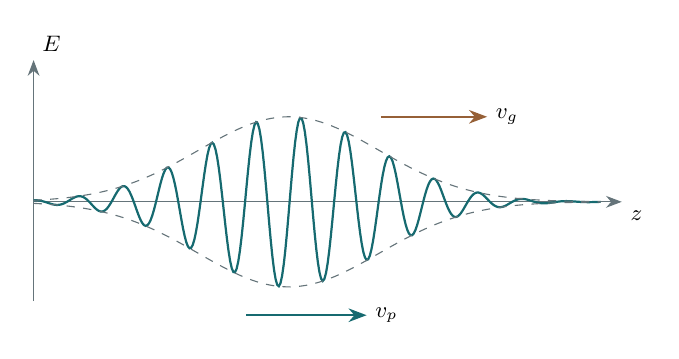
\begin{tikzpicture}[scale=.9,transform shape]
\draw[axis] (0.00000,0.00000)--(8.30000,0.00000);\draw[axis] (0.00000,-1.40000)--(0.00000,2.00000);\node[below right] at (8.30000,0.00000) {$z$};\node[above right] at (0.00000,2.00000) {$E$};\draw[traj] plot coordinates {(0.00000,0.02198) (0.02292,0.02252) (0.04585,0.02181) (0.06877,0.01976) (0.09169,0.01635) (0.11461,0.01164) (0.13754,0.00576) (0.16046,-0.00105) (0.18338,-0.00850) (0.20630,-0.01621) (0.22923,-0.02377) (0.25215,-0.03072) (0.27507,-0.03658) (0.29799,-0.04093) (0.32092,-0.04334) (0.34384,-0.04351) (0.36676,-0.04120) (0.38968,-0.03630) (0.41261,-0.02886) (0.43553,-0.01907) (0.45845,-0.00728) (0.48138,0.00603) (0.50430,0.02023) (0.52722,0.03457) (0.55014,0.04824) (0.57307,0.06041) (0.59599,0.07022) (0.61891,0.07692) (0.64183,0.07984) (0.66476,0.07849) (0.68768,0.07258) (0.71060,0.06205) (0.73352,0.04711) (0.75645,0.02824) (0.77937,0.00620) (0.80229,-0.01802) (0.82521,-0.04322) (0.84814,-0.06804) (0.87106,-0.09105) (0.89398,-0.11078) (0.91691,-0.12585) (0.93983,-0.13505) (0.96275,-0.13738) (0.98567,-0.13219) (1.00860,-0.11920) (1.03152,-0.09854) (1.05444,-0.07081) (1.07736,-0.03705) (1.10029,0.00127) (1.12321,0.04234) (1.14613,0.08402) (1.16905,0.12402) (1.19198,0.15996) (1.21490,0.18953) (1.23782,0.21063) (1.26074,0.22147) (1.28367,0.22077) (1.30659,0.20776) (1.32951,0.18236) (1.35244,0.14516) (1.37536,0.09749) (1.39828,0.04132) (1.42120,-0.02074) (1.44413,-0.08560) (1.46705,-0.14982) (1.48997,-0.20976) (1.51289,-0.26183) (1.53582,-0.30264) (1.55874,-0.32923) (1.58166,-0.33929) (1.60458,-0.33128) (1.62751,-0.30460) (1.65043,-0.25965) (1.67335,-0.19791) (1.69628,-0.12185) (1.71920,-0.03491) (1.74212,0.05871) (1.76504,0.15416) (1.78797,0.24626) (1.81089,0.32975) (1.83381,0.39956) (1.85673,0.45113) (1.87966,0.48069) (1.90258,0.48551) (1.92550,0.46410) (1.94842,0.41638) (1.97135,0.34371) (1.99427,0.24891) (2.01719,0.13618) (2.04011,0.01088) (2.06304,-0.12067) (2.08596,-0.25152) (2.10888,-0.37445) (2.13181,-0.48238) (2.15473,-0.56876) (2.17765,-0.62795) (2.20057,-0.65558) (2.22350,-0.64888) (2.24642,-0.60684) (2.26934,-0.53037) (2.29226,-0.42234) (2.31519,-0.28744) (2.33811,-0.13204) (2.36103,0.03613) (2.38395,0.20835) (2.40688,0.37538) (2.42980,0.52794) (2.45272,0.65725) (2.47564,0.75549) (2.49857,0.81631) (2.52149,0.83522) (2.54441,0.80988) (2.56734,0.74032) (2.59026,0.62901) (2.61318,0.48075) (2.63610,0.30254) (2.65903,0.10321) (2.68195,-0.10703) (2.70487,-0.31707) (2.72779,-0.51555) (2.75072,-0.69145) (2.77364,-0.83468) (2.79656,-0.93675) (2.81948,-0.99117) (2.84241,-0.99394) (2.86533,-0.94378) (2.88825,-0.84228) (2.91117,-0.69384) (2.93410,-0.50554) (2.95702,-0.28675) (2.97994,-0.04869) (3.00287,0.19617) (3.02579,0.43478) (3.04871,0.65420) (3.07163,0.84233) (3.09456,0.98858) (3.11748,1.08448) (3.14040,1.12418) (3.16332,1.10480) (3.18625,1.02663) (3.20917,0.89316) (3.23209,0.71090) (3.25501,0.48911) (3.27794,0.23926) (3.30086,-0.02553) (3.32378,-0.29122) (3.34670,-0.54361) (3.36963,-0.76909) (3.39255,-0.95543) (3.41547,-1.09242) (3.43840,-1.17248) (3.46132,-1.19105) (3.48424,-1.14688) (3.50716,-1.04210) (3.53009,-0.88212) (3.55301,-0.67536) (3.57593,-0.43275) (3.59885,-0.16719) (3.62178,0.10718) (3.64470,0.37574) (3.66762,0.62420) (3.69054,0.83936) (3.71347,1.00984) (3.73639,1.12672) (3.75931,1.18396) (3.78223,1.17875) (3.80516,1.11169) (3.82808,0.98667) (3.85100,0.81068) (3.87393,0.59341) (3.89685,0.34670) (3.91977,0.08388) (3.94269,-0.18098) (3.96562,-0.43379) (3.98854,-0.66128) (4.01146,-0.85165) (4.03438,-0.99522) (4.05731,-1.08494) (4.08023,-1.11673) (4.10315,-1.08966) (4.12607,-1.00598) (4.14900,-0.87093) (4.17192,-0.69242) (4.19484,-0.48059) (4.21777,-0.24717) (4.24069,-0.00489) (4.26361,0.23330) (4.28653,0.45487) (4.30946,0.64842) (4.33238,0.80428) (4.35530,0.91496) (4.37822,0.97555) (4.40115,0.98393) (4.42407,0.94079) (4.44699,0.84958) (4.46991,0.71623) (4.49284,0.54877) (4.51576,0.35689) (4.53868,0.15132) (4.56160,-0.05675) (4.58453,-0.25628) (4.60745,-0.43697) (4.63037,-0.58982) (4.65330,-0.70757) (4.67622,-0.78501) (4.69914,-0.81926) (4.72206,-0.80981) (4.74499,-0.75851) (4.76791,-0.66937) (4.79083,-0.54829) (4.81375,-0.40270) (4.83668,-0.24107) (4.85960,-0.07246) (4.88252,0.09401) (4.90544,0.24966) (4.92837,0.38668) (4.95129,0.49854) (4.97421,0.58028) (4.99713,0.62874) (5.02006,0.64263) (5.04298,0.62257) (5.06590,0.57096) (5.08883,0.49177) (5.11175,0.39029) (5.13467,0.27278) (5.15759,0.14609) (5.18052,0.01727) (5.20344,-0.10681) (5.22636,-0.21984) (5.24928,-0.31636) (5.27221,-0.39205) (5.29513,-0.44387) (5.31805,-0.47021) (5.34097,-0.47087) (5.36390,-0.44704) (5.38682,-0.40116) (5.40974,-0.33670) (5.43266,-0.25797) (5.45559,-0.16982) (5.47851,-0.07736) (5.50143,0.01433) (5.52436,0.10047) (5.54728,0.17683) (5.57020,0.23991) (5.59312,0.28711) (5.61605,0.31681) (5.63897,0.32840) (5.66189,0.32229) (5.68481,0.29978) (5.70774,0.26299) (5.73066,0.21467) (5.75358,0.15802) (5.77650,0.09651) (5.79943,0.03367) (5.82235,-0.02714) (5.84527,-0.08282) (5.86819,-0.13078) (5.89112,-0.16896) (5.91404,-0.19596) (5.93696,-0.21106) (5.95989,-0.21423) (5.98281,-0.20606) (6.00573,-0.18770) (6.02865,-0.16080) (6.05158,-0.12732) (6.07450,-0.08947) (6.09742,-0.04952) (6.12034,-0.00973) (6.14327,0.02783) (6.16619,0.06134) (6.18911,0.08931) (6.21203,0.11065) (6.23496,0.12472) (6.25788,0.13128) (6.28080,0.13054) (6.30372,0.12305) (6.32665,0.10971) (6.34957,0.09165) (6.37249,0.07017) (6.39542,0.04665) (6.41834,0.02249) (6.44126,-0.00099) (6.46418,-0.02260) (6.48711,-0.04135) (6.51003,-0.05648) (6.53295,-0.06746) (6.55587,-0.07406) (6.57880,-0.07626) (6.60172,-0.07430) (6.62464,-0.06863) (6.64756,-0.05984) (6.67049,-0.04866) (6.69341,-0.03586) (6.71633,-0.02227) (6.73926,-0.00866) (6.76218,0.00425) (6.78510,0.01582) (6.80802,0.02558) (6.83095,0.03315) (6.85387,0.03832) (6.87679,0.04104) (6.89971,0.04137) (6.92264,0.03951) (6.94556,0.03574) (6.96848,0.03045) (6.99140,0.02404) (7.01433,0.01696) (7.03725,0.00965) (7.06017,0.00250) (7.08309,-0.00410) (7.10602,-0.00988) (7.12894,-0.01459) (7.15186,-0.01808) (7.17479,-0.02030) (7.19771,-0.02123) (7.22063,-0.02096) (7.24355,-0.01962) (7.26648,-0.01738) (7.28940,-0.01445) (7.31232,-0.01104) (7.33524,-0.00740) (7.35817,-0.00373) (7.38109,-0.00024) (7.40401,0.00291) (7.42693,0.00559) (7.44986,0.00769) (7.47278,0.00918) (7.49570,0.01003) (7.51862,0.01026) (7.54155,0.00992) (7.56447,0.00910) (7.58739,0.00789) (7.61032,0.00639) (7.63324,0.00471) (7.65616,0.00296) (7.67908,0.00125) (7.70201,-0.00034) (7.72493,-0.00174) (7.74785,-0.00289) (7.77077,-0.00376) (7.79370,-0.00434) (7.81662,-0.00462) (7.83954,-0.00463) (7.86246,-0.00439) (7.88539,-0.00394) (7.90831,-0.00334) (7.93123,-0.00263) (7.95415,-0.00186) (7.97708,-0.00108) (8.00000,-0.00034)};\draw[guide] plot coordinates {(0.00000,0.02198) (0.02292,0.02312) (0.04585,0.02432) (0.06877,0.02557) (0.09169,0.02688) (0.11461,0.02824) (0.13754,0.02966) (0.16046,0.03115) (0.18338,0.03269) (0.20630,0.03431) (0.22923,0.03599) (0.25215,0.03774) (0.27507,0.03957) (0.29799,0.04147) (0.32092,0.04344) (0.34384,0.04550) (0.36676,0.04764) (0.38968,0.04986) (0.41261,0.05217) (0.43553,0.05456) (0.45845,0.05705) (0.48138,0.05964) (0.50430,0.06232) (0.52722,0.06510) (0.55014,0.06798) (0.57307,0.07097) (0.59599,0.07406) (0.61891,0.07726) (0.64183,0.08058) (0.66476,0.08401) (0.68768,0.08756) (0.71060,0.09123) (0.73352,0.09502) (0.75645,0.09893) (0.77937,0.10298) (0.80229,0.10716) (0.82521,0.11146) (0.84814,0.11591) (0.87106,0.12049) (0.89398,0.12522) (0.91691,0.13008) (0.93983,0.13509) (0.96275,0.14025) (0.98567,0.14556) (1.00860,0.15102) (1.03152,0.15664) (1.05444,0.16241) (1.07736,0.16834) (1.10029,0.17443) (1.12321,0.18068) (1.14613,0.18709) (1.16905,0.19367) (1.19198,0.20042) (1.21490,0.20733) (1.23782,0.21441) (1.26074,0.22166) (1.28367,0.22908) (1.30659,0.23668) (1.32951,0.24445) (1.35244,0.25239) (1.37536,0.26050) (1.39828,0.26879) (1.42120,0.27725) (1.44413,0.28588) (1.46705,0.29469) (1.48997,0.30367) (1.51289,0.31282) (1.53582,0.32214) (1.55874,0.33164) (1.58166,0.34130) (1.60458,0.35113) (1.62751,0.36113) (1.65043,0.37129) (1.67335,0.38161) (1.69628,0.39210) (1.71920,0.40274) (1.74212,0.41353) (1.76504,0.42448) (1.78797,0.43557) (1.81089,0.44681) (1.83381,0.45819) (1.85673,0.46971) (1.87966,0.48136) (1.90258,0.49315) (1.92550,0.50505) (1.94842,0.51708) (1.97135,0.52922) (1.99427,0.54147) (2.01719,0.55382) (2.04011,0.56627) (2.06304,0.57882) (2.08596,0.59145) (2.10888,0.60416) (2.13181,0.61694) (2.15473,0.62979) (2.17765,0.64269) (2.20057,0.65565) (2.22350,0.66866) (2.24642,0.68170) (2.26934,0.69477) (2.29226,0.70786) (2.31519,0.72096) (2.33811,0.73407) (2.36103,0.74717) (2.38395,0.76027) (2.40688,0.77333) (2.42980,0.78637) (2.45272,0.79937) (2.47564,0.81232) (2.49857,0.82522) (2.52149,0.83804) (2.54441,0.85079) (2.56734,0.86346) (2.59026,0.87602) (2.61318,0.88848) (2.63610,0.90083) (2.65903,0.91305) (2.68195,0.92514) (2.70487,0.93709) (2.72779,0.94888) (2.75072,0.96050) (2.77364,0.97196) (2.79656,0.98323) (2.81948,0.99431) (2.84241,1.00519) (2.86533,1.01586) (2.88825,1.02631) (2.91117,1.03653) (2.93410,1.04651) (2.95702,1.05625) (2.97994,1.06573) (3.00287,1.07494) (3.02579,1.08389) (3.04871,1.09256) (3.07163,1.10093) (3.09456,1.10901) (3.11748,1.11679) (3.14040,1.12426) (3.16332,1.13141) (3.18625,1.13824) (3.20917,1.14474) (3.23209,1.15090) (3.25501,1.15672) (3.27794,1.16219) (3.30086,1.16731) (3.32378,1.17207) (3.34670,1.17647) (3.36963,1.18050) (3.39255,1.18417) (3.41547,1.18745) (3.43840,1.19037) (3.46132,1.19290) (3.48424,1.19505) (3.50716,1.19681) (3.53009,1.19819) (3.55301,1.19918) (3.57593,1.19979) (3.59885,1.20000) (3.62178,1.19982) (3.64470,1.19926) (3.66762,1.19831) (3.69054,1.19697) (3.71347,1.19524) (3.73639,1.19313) (3.75931,1.19064) (3.78223,1.18776) (3.80516,1.18451) (3.82808,1.18089) (3.85100,1.17689) (3.87393,1.17253) (3.89685,1.16780) (3.91977,1.16272) (3.94269,1.15728) (3.96562,1.15150) (3.98854,1.14537) (4.01146,1.13891) (4.03438,1.13211) (4.05731,1.12499) (4.08023,1.11755) (4.10315,1.10981) (4.12607,1.10175) (4.14900,1.09341) (4.17192,1.08477) (4.19484,1.07585) (4.21777,1.06666) (4.24069,1.05721) (4.26361,1.04750) (4.28653,1.03754) (4.30946,1.02734) (4.33238,1.01691) (4.35530,1.00627) (4.37822,0.99541) (4.40115,0.98435) (4.42407,0.97309) (4.44699,0.96166) (4.46991,0.95005) (4.49284,0.93827) (4.51576,0.92634) (4.53868,0.91427) (4.56160,0.90206) (4.58453,0.88972) (4.60745,0.87727) (4.63037,0.86472) (4.65330,0.85206) (4.67622,0.83932) (4.69914,0.82650) (4.72206,0.81362) (4.74499,0.80067) (4.76791,0.78768) (4.79083,0.77464) (4.81375,0.76157) (4.83668,0.74848) (4.85960,0.73538) (4.88252,0.72227) (4.90544,0.70917) (4.92837,0.69608) (4.95129,0.68300) (4.97421,0.66996) (4.99713,0.65695) (5.02006,0.64399) (5.04298,0.63108) (5.06590,0.61822) (5.08883,0.60543) (5.11175,0.59271) (5.13467,0.58008) (5.15759,0.56752) (5.18052,0.55506) (5.20344,0.54270) (5.22636,0.53044) (5.24928,0.51829) (5.27221,0.50625) (5.29513,0.49433) (5.31805,0.48254) (5.34097,0.47087) (5.36390,0.45934) (5.38682,0.44794) (5.40974,0.43669) (5.43266,0.42558) (5.45559,0.41462) (5.47851,0.40381) (5.50143,0.39315) (5.52436,0.38265) (5.54728,0.37231) (5.57020,0.36214) (5.59312,0.35212) (5.61605,0.34228) (5.63897,0.33260) (5.66189,0.32309) (5.68481,0.31374) (5.70774,0.30458) (5.73066,0.29558) (5.75358,0.28675) (5.77650,0.27810) (5.79943,0.26962) (5.82235,0.26132) (5.84527,0.25319) (5.86819,0.24523) (5.89112,0.23745) (5.91404,0.22984) (5.93696,0.22240) (5.95989,0.21513) (5.98281,0.20803) (6.00573,0.20110) (6.02865,0.19434) (6.05158,0.18774) (6.07450,0.18131) (6.09742,0.17504) (6.12034,0.16894) (6.14327,0.16299) (6.16619,0.15721) (6.18911,0.15158) (6.21203,0.14610) (6.23496,0.14078) (6.25788,0.13560) (6.28080,0.13058) (6.30372,0.12570) (6.32665,0.12096) (6.34957,0.11636) (6.37249,0.11190) (6.39542,0.10758) (6.41834,0.10339) (6.44126,0.09933) (6.46418,0.09540) (6.48711,0.09160) (6.51003,0.08792) (6.53295,0.08436) (6.55587,0.08092) (6.57880,0.07759) (6.60172,0.07437) (6.62464,0.07127) (6.64756,0.06827) (6.67049,0.06538) (6.69341,0.06259) (6.71633,0.05990) (6.73926,0.05731) (6.76218,0.05481) (6.78510,0.05240) (6.80802,0.05008) (6.83095,0.04785) (6.85387,0.04571) (6.87679,0.04364) (6.89971,0.04166) (6.92264,0.03975) (6.94556,0.03792) (6.96848,0.03616) (6.99140,0.03447) (7.01433,0.03285) (7.03725,0.03130) (7.06017,0.02981) (7.08309,0.02838) (7.10602,0.02701) (7.12894,0.02570) (7.15186,0.02444) (7.17479,0.02324) (7.19771,0.02209) (7.22063,0.02099) (7.24355,0.01994) (7.26648,0.01893) (7.28940,0.01797) (7.31232,0.01706) (7.33524,0.01618) (7.35817,0.01535) (7.38109,0.01455) (7.40401,0.01379) (7.42693,0.01306) (7.44986,0.01237) (7.47278,0.01172) (7.49570,0.01109) (7.51862,0.01049) (7.54155,0.00993) (7.56447,0.00939) (7.58739,0.00887) (7.61032,0.00838) (7.63324,0.00792) (7.65616,0.00748) (7.67908,0.00706) (7.70201,0.00666) (7.72493,0.00629) (7.74785,0.00593) (7.77077,0.00559) (7.79370,0.00527) (7.81662,0.00497) (7.83954,0.00468) (7.86246,0.00440) (7.88539,0.00415) (7.90831,0.00390) (7.93123,0.00367) (7.95415,0.00345) (7.97708,0.00324) (8.00000,0.00305)};\draw[guide] plot coordinates {(0.00000,-0.02198) (0.02292,-0.02312) (0.04585,-0.02432) (0.06877,-0.02557) (0.09169,-0.02688) (0.11461,-0.02824) (0.13754,-0.02966) (0.16046,-0.03115) (0.18338,-0.03269) (0.20630,-0.03431) (0.22923,-0.03599) (0.25215,-0.03774) (0.27507,-0.03957) (0.29799,-0.04147) (0.32092,-0.04344) (0.34384,-0.04550) (0.36676,-0.04764) (0.38968,-0.04986) (0.41261,-0.05217) (0.43553,-0.05456) (0.45845,-0.05705) (0.48138,-0.05964) (0.50430,-0.06232) (0.52722,-0.06510) (0.55014,-0.06798) (0.57307,-0.07097) (0.59599,-0.07406) (0.61891,-0.07726) (0.64183,-0.08058) (0.66476,-0.08401) (0.68768,-0.08756) (0.71060,-0.09123) (0.73352,-0.09502) (0.75645,-0.09893) (0.77937,-0.10298) (0.80229,-0.10716) (0.82521,-0.11146) (0.84814,-0.11591) (0.87106,-0.12049) (0.89398,-0.12522) (0.91691,-0.13008) (0.93983,-0.13509) (0.96275,-0.14025) (0.98567,-0.14556) (1.00860,-0.15102) (1.03152,-0.15664) (1.05444,-0.16241) (1.07736,-0.16834) (1.10029,-0.17443) (1.12321,-0.18068) (1.14613,-0.18709) (1.16905,-0.19367) (1.19198,-0.20042) (1.21490,-0.20733) (1.23782,-0.21441) (1.26074,-0.22166) (1.28367,-0.22908) (1.30659,-0.23668) (1.32951,-0.24445) (1.35244,-0.25239) (1.37536,-0.26050) (1.39828,-0.26879) (1.42120,-0.27725) (1.44413,-0.28588) (1.46705,-0.29469) (1.48997,-0.30367) (1.51289,-0.31282) (1.53582,-0.32214) (1.55874,-0.33164) (1.58166,-0.34130) (1.60458,-0.35113) (1.62751,-0.36113) (1.65043,-0.37129) (1.67335,-0.38161) (1.69628,-0.39210) (1.71920,-0.40274) (1.74212,-0.41353) (1.76504,-0.42448) (1.78797,-0.43557) (1.81089,-0.44681) (1.83381,-0.45819) (1.85673,-0.46971) (1.87966,-0.48136) (1.90258,-0.49315) (1.92550,-0.50505) (1.94842,-0.51708) (1.97135,-0.52922) (1.99427,-0.54147) (2.01719,-0.55382) (2.04011,-0.56627) (2.06304,-0.57882) (2.08596,-0.59145) (2.10888,-0.60416) (2.13181,-0.61694) (2.15473,-0.62979) (2.17765,-0.64269) (2.20057,-0.65565) (2.22350,-0.66866) (2.24642,-0.68170) (2.26934,-0.69477) (2.29226,-0.70786) (2.31519,-0.72096) (2.33811,-0.73407) (2.36103,-0.74717) (2.38395,-0.76027) (2.40688,-0.77333) (2.42980,-0.78637) (2.45272,-0.79937) (2.47564,-0.81232) (2.49857,-0.82522) (2.52149,-0.83804) (2.54441,-0.85079) (2.56734,-0.86346) (2.59026,-0.87602) (2.61318,-0.88848) (2.63610,-0.90083) (2.65903,-0.91305) (2.68195,-0.92514) (2.70487,-0.93709) (2.72779,-0.94888) (2.75072,-0.96050) (2.77364,-0.97196) (2.79656,-0.98323) (2.81948,-0.99431) (2.84241,-1.00519) (2.86533,-1.01586) (2.88825,-1.02631) (2.91117,-1.03653) (2.93410,-1.04651) (2.95702,-1.05625) (2.97994,-1.06573) (3.00287,-1.07494) (3.02579,-1.08389) (3.04871,-1.09256) (3.07163,-1.10093) (3.09456,-1.10901) (3.11748,-1.11679) (3.14040,-1.12426) (3.16332,-1.13141) (3.18625,-1.13824) (3.20917,-1.14474) (3.23209,-1.15090) (3.25501,-1.15672) (3.27794,-1.16219) (3.30086,-1.16731) (3.32378,-1.17207) (3.34670,-1.17647) (3.36963,-1.18050) (3.39255,-1.18417) (3.41547,-1.18745) (3.43840,-1.19037) (3.46132,-1.19290) (3.48424,-1.19505) (3.50716,-1.19681) (3.53009,-1.19819) (3.55301,-1.19918) (3.57593,-1.19979) (3.59885,-1.20000) (3.62178,-1.19982) (3.64470,-1.19926) (3.66762,-1.19831) (3.69054,-1.19697) (3.71347,-1.19524) (3.73639,-1.19313) (3.75931,-1.19064) (3.78223,-1.18776) (3.80516,-1.18451) (3.82808,-1.18089) (3.85100,-1.17689) (3.87393,-1.17253) (3.89685,-1.16780) (3.91977,-1.16272) (3.94269,-1.15728) (3.96562,-1.15150) (3.98854,-1.14537) (4.01146,-1.13891) (4.03438,-1.13211) (4.05731,-1.12499) (4.08023,-1.11755) (4.10315,-1.10981) (4.12607,-1.10175) (4.14900,-1.09341) (4.17192,-1.08477) (4.19484,-1.07585) (4.21777,-1.06666) (4.24069,-1.05721) (4.26361,-1.04750) (4.28653,-1.03754) (4.30946,-1.02734) (4.33238,-1.01691) (4.35530,-1.00627) (4.37822,-0.99541) (4.40115,-0.98435) (4.42407,-0.97309) (4.44699,-0.96166) (4.46991,-0.95005) (4.49284,-0.93827) (4.51576,-0.92634) (4.53868,-0.91427) (4.56160,-0.90206) (4.58453,-0.88972) (4.60745,-0.87727) (4.63037,-0.86472) (4.65330,-0.85206) (4.67622,-0.83932) (4.69914,-0.82650) (4.72206,-0.81362) (4.74499,-0.80067) (4.76791,-0.78768) (4.79083,-0.77464) (4.81375,-0.76157) (4.83668,-0.74848) (4.85960,-0.73538) (4.88252,-0.72227) (4.90544,-0.70917) (4.92837,-0.69608) (4.95129,-0.68300) (4.97421,-0.66996) (4.99713,-0.65695) (5.02006,-0.64399) (5.04298,-0.63108) (5.06590,-0.61822) (5.08883,-0.60543) (5.11175,-0.59271) (5.13467,-0.58008) (5.15759,-0.56752) (5.18052,-0.55506) (5.20344,-0.54270) (5.22636,-0.53044) (5.24928,-0.51829) (5.27221,-0.50625) (5.29513,-0.49433) (5.31805,-0.48254) (5.34097,-0.47087) (5.36390,-0.45934) (5.38682,-0.44794) (5.40974,-0.43669) (5.43266,-0.42558) (5.45559,-0.41462) (5.47851,-0.40381) (5.50143,-0.39315) (5.52436,-0.38265) (5.54728,-0.37231) (5.57020,-0.36214) (5.59312,-0.35212) (5.61605,-0.34228) (5.63897,-0.33260) (5.66189,-0.32309) (5.68481,-0.31374) (5.70774,-0.30458) (5.73066,-0.29558) (5.75358,-0.28675) (5.77650,-0.27810) (5.79943,-0.26962) (5.82235,-0.26132) (5.84527,-0.25319) (5.86819,-0.24523) (5.89112,-0.23745) (5.91404,-0.22984) (5.93696,-0.22240) (5.95989,-0.21513) (5.98281,-0.20803) (6.00573,-0.20110) (6.02865,-0.19434) (6.05158,-0.18774) (6.07450,-0.18131) (6.09742,-0.17504) (6.12034,-0.16894) (6.14327,-0.16299) (6.16619,-0.15721) (6.18911,-0.15158) (6.21203,-0.14610) (6.23496,-0.14078) (6.25788,-0.13560) (6.28080,-0.13058) (6.30372,-0.12570) (6.32665,-0.12096) (6.34957,-0.11636) (6.37249,-0.11190) (6.39542,-0.10758) (6.41834,-0.10339) (6.44126,-0.09933) (6.46418,-0.09540) (6.48711,-0.09160) (6.51003,-0.08792) (6.53295,-0.08436) (6.55587,-0.08092) (6.57880,-0.07759) (6.60172,-0.07437) (6.62464,-0.07127) (6.64756,-0.06827) (6.67049,-0.06538) (6.69341,-0.06259) (6.71633,-0.05990) (6.73926,-0.05731) (6.76218,-0.05481) (6.78510,-0.05240) (6.80802,-0.05008) (6.83095,-0.04785) (6.85387,-0.04571) (6.87679,-0.04364) (6.89971,-0.04166) (6.92264,-0.03975) (6.94556,-0.03792) (6.96848,-0.03616) (6.99140,-0.03447) (7.01433,-0.03285) (7.03725,-0.03130) (7.06017,-0.02981) (7.08309,-0.02838) (7.10602,-0.02701) (7.12894,-0.02570) (7.15186,-0.02444) (7.17479,-0.02324) (7.19771,-0.02209) (7.22063,-0.02099) (7.24355,-0.01994) (7.26648,-0.01893) (7.28940,-0.01797) (7.31232,-0.01706) (7.33524,-0.01618) (7.35817,-0.01535) (7.38109,-0.01455) (7.40401,-0.01379) (7.42693,-0.01306) (7.44986,-0.01237) (7.47278,-0.01172) (7.49570,-0.01109) (7.51862,-0.01049) (7.54155,-0.00993) (7.56447,-0.00939) (7.58739,-0.00887) (7.61032,-0.00838) (7.63324,-0.00792) (7.65616,-0.00748) (7.67908,-0.00706) (7.70201,-0.00666) (7.72493,-0.00629) (7.74785,-0.00593) (7.77077,-0.00559) (7.79370,-0.00527) (7.81662,-0.00497) (7.83954,-0.00468) (7.86246,-0.00440) (7.88539,-0.00415) (7.90831,-0.00390) (7.93123,-0.00367) (7.95415,-0.00345) (7.97708,-0.00324) (8.00000,-0.00305)};\draw[force] (4.90000,1.20000)--(6.40000,1.20000);\node[right] at (6.40000,1.20000) {$v_g$};\draw[motion] (3.00000,-1.60000)--(4.70000,-1.60000);\node[right] at (4.70000,-1.60000) {$v_p$};
\end{tikzpicture}
\figcaption{图光5.1\quad 载波与外包络具有不同的传播速度。}
\end{minipage}\end{center}

\Needspace{6\baselineskip}\subsection*{解答}


图光5.1的细密波峰表示载波相位，虚线包络表示相邻频率分量叠加后的振幅。用真空波长$\lambda_0$表示题给色散，介质内波长记为$\lambda_m$，二者分别满足$\lambda_0\omega=2\pi c$、$\lambda_mk=2\pi$。先把两种速度都写在同一条$k(\omega)$色散关系上：
\[
k(\omega)=\frac{n(\omega)\omega}{c},\quad
v_p=\frac{\omega}{k}=\frac cn,\quad
\frac1{v_g}=\frac{\dd k}{\dd\omega}=\frac1c\left(n+\omega\frac{\dd n}{\dd\omega}\right).
\]
窄带波包可把$k(\omega)$在中心频率展开到一次，包络沿$z-v_gt$移动。由$\dd\lambda_0/\dd\omega=-\lambda_0/\omega$，有$\omega\,\dd n/\dd\omega=-\lambda_0\,\dd n/\dd\lambda_0$，因此
\[
n_g=n-\lambda_0 n',\qquad \boxed{v_g=\frac c{n-\lambda_0 n'}}.
\]
下面把题给$n_D$作为589.3nm处的局部折射率，并保留柯西式给定的斜率。具体做法是先算$n_{\rm fit}(589.3)=1.51562655$，与$n_D=1.51630$相差$\Delta A=.0006734503$，再把常数项校准为$A_c=A+\Delta A=1.5046734503$。校准式$n_c(\lambda_0)=A_c+B/\lambda_0^2+C/\lambda_0^4$在589.3nm处取$n_D$，导数仍由$B,C$给出：$n'=-2B/\lambda_0^3-4C/\lambda_0^5$。

在$\lambda_0=589.3\,\mathrm{nm}$处，用nm作为求导长度单位，有
\[
n'=-3.55556\times10^{-5}\,\mathrm{nm^{-1}},\qquad
-\lambda_0 n'=0.0209529.
\]
其中$n'$的单位为$\mathrm{nm^{-1}}$，与以nm写的$\lambda_0$相乘后无量纲。解图光5.1B画出校准后的$n_c$与$n_g$；在所示可见光区间$n'<0$，所以$n_g-n=-\lambda_0n'>0$。
\begin{center}\begin{minipage}{.98\linewidth}\centering
\begin{tikzpicture}[scale=.88,transform shape]
\draw[axis] (0,0)--(7.3,0) node[right] {$\lambda_0/{\rm nm}$};
\draw[axis] (0,0)--(0,2.8);
\node[above left] at (0,2.8) {$\text{折射率}$};
\draw[thin] (0.000000,0)--(0.000000,-0.06);\node[below,font=\scriptsize] at (0.000000,-0.08) {$ 420 $};
\draw[thin] (1.473684,0)--(1.473684,-0.06);\node[below,font=\scriptsize] at (1.473684,-0.08) {$ 500 $};
\draw[thin] (3.118684,0)--(3.118684,-0.06);\node[below,font=\scriptsize] at (3.118684,-0.08) {$ 589.3 $};
\draw[thin] (5.157895,0)--(5.157895,-0.06);\node[below,font=\scriptsize] at (5.157895,-0.08) {$ 700 $};
\draw[thin] (7.000000,0)--(7.000000,-0.06);\node[below,font=\scriptsize] at (7.000000,-0.08) {$ 800 $};
\draw[thin] (0,0.000000)--(-.06,0.000000);\node[left,font=\scriptsize] at (-.08,0.000000) {$ 1.5 $};
\draw[thin] (0,0.625000)--(-.06,0.625000);\node[left,font=\scriptsize] at (-.08,0.625000) {$ 1.52 $};
\draw[thin] (0,1.250000)--(-.06,1.250000);\node[left,font=\scriptsize] at (-.08,1.250000) {$ 1.54 $};
\draw[thin] (0,1.875000)--(-.06,1.875000);\node[left,font=\scriptsize] at (-.08,1.875000) {$ 1.56 $};
\draw[thin] (0,2.500000)--(-.06,2.500000);\node[left,font=\scriptsize] at (-.08,2.500000) {$ 1.58 $};
\draw[thick,color=accent] plot coordinates {(0.0000000,0.7927855) (0.0291667,0.7889732) (0.0583333,0.7851882) (0.0875000,0.7814304) (0.1166667,0.7776997) (0.1458333,0.7739959) (0.1750000,0.7703190) (0.2041667,0.7666687) (0.2333333,0.7630449) (0.2625000,0.7594475) (0.2916667,0.7558764) (0.3208333,0.7523313) (0.3500000,0.7488122) (0.3791667,0.7453189) (0.4083333,0.7418512) (0.4375000,0.7384090) (0.4666667,0.7349922) (0.4958333,0.7316005) (0.5250000,0.7282338) (0.5541667,0.7248919) (0.5833333,0.7215748) (0.6125000,0.7182821) (0.6416667,0.7150138) (0.6708333,0.7117697) (0.7000000,0.7085496) (0.7291667,0.7053534) (0.7583333,0.7021808) (0.7875000,0.6990318) (0.8166667,0.6959061) (0.8458333,0.6928036) (0.8750000,0.6897241) (0.9041667,0.6866675) (0.9333333,0.6836335) (0.9625000,0.6806221) (0.9916667,0.6776330) (1.0208333,0.6746660) (1.0500000,0.6717211) (1.0791667,0.6687980) (1.1083333,0.6658966) (1.1375000,0.6630166) (1.1666667,0.6601580) (1.1958333,0.6573206) (1.2250000,0.6545042) (1.2541667,0.6517086) (1.2833333,0.6489337) (1.3125000,0.6461794) (1.3416667,0.6434453) (1.3708333,0.6407315) (1.4000000,0.6380377) (1.4291667,0.6353637) (1.4583333,0.6327094) (1.4875000,0.6300747) (1.5166667,0.6274594) (1.5458333,0.6248633) (1.5750000,0.6222863) (1.6041667,0.6197282) (1.6333333,0.6171888) (1.6625000,0.6146681) (1.6916667,0.6121658) (1.7208333,0.6096818) (1.7500000,0.6072160) (1.7791667,0.6047682) (1.8083333,0.6023382) (1.8375000,0.5999259) (1.8666667,0.5975312) (1.8958333,0.5951539) (1.9250000,0.5927938) (1.9541667,0.5904509) (1.9833333,0.5881250) (2.0125000,0.5858159) (2.0416667,0.5835234) (2.0708333,0.5812476) (2.1000000,0.5789881) (2.1291667,0.5767449) (2.1583333,0.5745179) (2.1875000,0.5723069) (2.2166667,0.5701117) (2.2458333,0.5679323) (2.2750000,0.5657685) (2.3041667,0.5636201) (2.3333333,0.5614871) (2.3625000,0.5593693) (2.3916667,0.5572666) (2.4208333,0.5551788) (2.4500000,0.5531059) (2.4791667,0.5510476) (2.5083333,0.5490040) (2.5375000,0.5469748) (2.5666667,0.5449599) (2.5958333,0.5429592) (2.6250000,0.5409727) (2.6541667,0.5390001) (2.6833333,0.5370413) (2.7125000,0.5350963) (2.7416667,0.5331650) (2.7708333,0.5312471) (2.8000000,0.5293426) (2.8291667,0.5274514) (2.8583333,0.5255733) (2.8875000,0.5237084) (2.9166667,0.5218563) (2.9458333,0.5200171) (2.9750000,0.5181906) (3.0041667,0.5163768) (3.0333333,0.5145754) (3.0625000,0.5127865) (3.0916667,0.5110098) (3.1208333,0.5092454) (3.1500000,0.5074931) (3.1791667,0.5057527) (3.2083333,0.5040243) (3.2375000,0.5023076) (3.2666667,0.5006027) (3.2958333,0.4989093) (3.3250000,0.4972274) (3.3541667,0.4955570) (3.3833333,0.4938978) (3.4125000,0.4922499) (3.4416667,0.4906131) (3.4708333,0.4889873) (3.5000000,0.4873725) (3.5291667,0.4857685) (3.5583333,0.4841752) (3.5875000,0.4825927) (3.6166667,0.4810207) (3.6458333,0.4794591) (3.6750000,0.4779080) (3.7041667,0.4763672) (3.7333333,0.4748367) (3.7625000,0.4733162) (3.7916667,0.4718059) (3.8208333,0.4703055) (3.8500000,0.4688150) (3.8791667,0.4673344) (3.9083333,0.4658634) (3.9375000,0.4644021) (3.9666667,0.4629504) (3.9958333,0.4615082) (4.0250000,0.4600754) (4.0541667,0.4586520) (4.0833333,0.4572378) (4.1125000,0.4558328) (4.1416667,0.4544369) (4.1708333,0.4530501) (4.2000000,0.4516722) (4.2291667,0.4503032) (4.2583333,0.4489431) (4.2875000,0.4475916) (4.3166667,0.4462489) (4.3458333,0.4449148) (4.3750000,0.4435892) (4.4041667,0.4422721) (4.4333333,0.4409634) (4.4625000,0.4396630) (4.4916667,0.4383709) (4.5208333,0.4370870) (4.5500000,0.4358112) (4.5791667,0.4345435) (4.6083333,0.4332838) (4.6375000,0.4320320) (4.6666667,0.4307881) (4.6958333,0.4295521) (4.7250000,0.4283238) (4.7541667,0.4271031) (4.7833333,0.4258901) (4.8125000,0.4246847) (4.8416667,0.4234868) (4.8708333,0.4222963) (4.9000000,0.4211132) (4.9291667,0.4199375) (4.9583333,0.4187690) (4.9875000,0.4176077) (5.0166667,0.4164537) (5.0458333,0.4153067) (5.0750000,0.4141667) (5.1041667,0.4130338) (5.1333333,0.4119078) (5.1625000,0.4107886) (5.1916667,0.4096763) (5.2208333,0.4085708) (5.2500000,0.4074720) (5.2791667,0.4063799) (5.3083333,0.4052944) (5.3375000,0.4042155) (5.3666667,0.4031431) (5.3958333,0.4020771) (5.4250000,0.4010176) (5.4541667,0.3999645) (5.4833333,0.3989176) (5.5125000,0.3978771) (5.5416667,0.3968427) (5.5708333,0.3958146) (5.6000000,0.3947925) (5.6291667,0.3937766) (5.6583333,0.3927667) (5.6875000,0.3917627) (5.7166667,0.3907648) (5.7458333,0.3897727) (5.7750000,0.3887864) (5.8041667,0.3878060) (5.8333333,0.3868314) (5.8625000,0.3858624) (5.8916667,0.3848992) (5.9208333,0.3839416) (5.9500000,0.3829895) (5.9791667,0.3820431) (6.0083333,0.3811021) (6.0375000,0.3801666) (6.0666667,0.3792365) (6.0958333,0.3783119) (6.1250000,0.3773925) (6.1541667,0.3764785) (6.1833333,0.3755698) (6.2125000,0.3746662) (6.2416667,0.3737679) (6.2708333,0.3728747) (6.3000000,0.3719867) (6.3291667,0.3711037) (6.3583333,0.3702257) (6.3875000,0.3693528) (6.4166667,0.3684848) (6.4458333,0.3676217) (6.4750000,0.3667635) (6.5041667,0.3659102) (6.5333333,0.3650617) (6.5625000,0.3642180) (6.5916667,0.3633791) (6.6208333,0.3625448) (6.6500000,0.3617153) (6.6791667,0.3608904) (6.7083333,0.3600701) (6.7375000,0.3592544) (6.7666667,0.3584432) (6.7958333,0.3576366) (6.8250000,0.3568344) (6.8541667,0.3560367) (6.8833333,0.3552434) (6.9125000,0.3544545) (6.9416667,0.3536699) (6.9708333,0.3528897) (7.0000000,0.3521137)};
\draw[thick,color=accent] (7.65,2.55)--(8.15,2.55);\node[right,font=\scriptsize] at (8.2,2.55) {$n$};
\draw[thick,dashed,color=warm] plot coordinates {(0.0000000,1.8076798) (0.0291667,1.8004045) (0.0583333,1.7931337) (0.0875000,1.7858689) (0.1166667,1.7786112) (0.1458333,1.7713620) (0.1750000,1.7641223) (0.2041667,1.7568935) (0.2333333,1.7496765) (0.2625000,1.7424724) (0.2916667,1.7352822) (0.3208333,1.7281068) (0.3500000,1.7209473) (0.3791667,1.7138044) (0.4083333,1.7066790) (0.4375000,1.6995719) (0.4666667,1.6924838) (0.4958333,1.6854155) (0.5250000,1.6783677) (0.5541667,1.6713409) (0.5833333,1.6643360) (0.6125000,1.6573534) (0.6416667,1.6503937) (0.6708333,1.6434575) (0.7000000,1.6365453) (0.7291667,1.6296575) (0.7583333,1.6227947) (0.7875000,1.6159573) (0.8166667,1.6091456) (0.8458333,1.6023601) (0.8750000,1.5956012) (0.9041667,1.5888692) (0.9333333,1.5821644) (0.9625000,1.5754871) (0.9916667,1.5688377) (1.0208333,1.5622164) (1.0500000,1.5556235) (1.0791667,1.5490591) (1.1083333,1.5425236) (1.1375000,1.5360172) (1.1666667,1.5295400) (1.1958333,1.5230922) (1.2250000,1.5166740) (1.2541667,1.5102855) (1.2833333,1.5039269) (1.3125000,1.4975983) (1.3416667,1.4912999) (1.3708333,1.4850316) (1.4000000,1.4787937) (1.4291667,1.4725862) (1.4583333,1.4664091) (1.4875000,1.4602626) (1.5166667,1.4541467) (1.5458333,1.4480614) (1.5750000,1.4420068) (1.6041667,1.4359829) (1.6333333,1.4299897) (1.6625000,1.4240272) (1.6916667,1.4180955) (1.7208333,1.4121945) (1.7500000,1.4063242) (1.7791667,1.4004846) (1.8083333,1.3946757) (1.8375000,1.3888975) (1.8666667,1.3831499) (1.8958333,1.3774328) (1.9250000,1.3717463) (1.9541667,1.3660903) (1.9833333,1.3604647) (2.0125000,1.3548695) (2.0416667,1.3493045) (2.0708333,1.3437698) (2.1000000,1.3382653) (2.1291667,1.3327909) (2.1583333,1.3273464) (2.1875000,1.3219319) (2.2166667,1.3165472) (2.2458333,1.3111923) (2.2750000,1.3058669) (2.3041667,1.3005712) (2.3333333,1.2953049) (2.3625000,1.2900679) (2.3916667,1.2848602) (2.4208333,1.2796816) (2.4500000,1.2745320) (2.4791667,1.2694114) (2.5083333,1.2643195) (2.5375000,1.2592563) (2.5666667,1.2542217) (2.5958333,1.2492155) (2.6250000,1.2442377) (2.6541667,1.2392880) (2.6833333,1.2343664) (2.7125000,1.2294727) (2.7416667,1.2246069) (2.7708333,1.2197687) (2.8000000,1.2149581) (2.8291667,1.2101750) (2.8583333,1.2054191) (2.8875000,1.2006904) (2.9166667,1.1959887) (2.9458333,1.1913139) (2.9750000,1.1866658) (3.0041667,1.1820444) (3.0333333,1.1774494) (3.0625000,1.1728808) (3.0916667,1.1683384) (3.1208333,1.1638220) (3.1500000,1.1593316) (3.1791667,1.1548670) (3.2083333,1.1504280) (3.2375000,1.1460145) (3.2666667,1.1416264) (3.2958333,1.1372635) (3.3250000,1.1329257) (3.3541667,1.1286128) (3.3833333,1.1243248) (3.4125000,1.1200614) (3.4416667,1.1158225) (3.4708333,1.1116080) (3.5000000,1.1074177) (3.5291667,1.1032516) (3.5583333,1.0991094) (3.5875000,1.0949910) (3.6166667,1.0908963) (3.6458333,1.0868251) (3.6750000,1.0827774) (3.7041667,1.0787529) (3.7333333,1.0747515) (3.7625000,1.0707731) (3.7916667,1.0668175) (3.8208333,1.0628846) (3.8500000,1.0589743) (3.8791667,1.0550864) (3.9083333,1.0512208) (3.9375000,1.0473774) (3.9666667,1.0435560) (3.9958333,1.0397564) (4.0250000,1.0359786) (4.0541667,1.0322224) (4.0833333,1.0284877) (4.1125000,1.0247743) (4.1416667,1.0210822) (4.1708333,1.0174111) (4.2000000,1.0137609) (4.2291667,1.0101316) (4.2583333,1.0065229) (4.2875000,1.0029348) (4.3166667,0.9993671) (4.3458333,0.9958197) (4.3750000,0.9922924) (4.4041667,0.9887852) (4.4333333,0.9852979) (4.4625000,0.9818303) (4.4916667,0.9783824) (4.5208333,0.9749540) (4.5500000,0.9715451) (4.5791667,0.9681554) (4.6083333,0.9647848) (4.6375000,0.9614333) (4.6666667,0.9581006) (4.6958333,0.9547868) (4.7250000,0.9514916) (4.7541667,0.9482149) (4.7833333,0.9449567) (4.8125000,0.9417167) (4.8416667,0.9384950) (4.8708333,0.9352913) (4.9000000,0.9321055) (4.9291667,0.9289376) (4.9583333,0.9257873) (4.9875000,0.9226547) (5.0166667,0.9195396) (5.0458333,0.9164418) (5.0750000,0.9133613) (5.1041667,0.9102979) (5.1333333,0.9072515) (5.1625000,0.9042221) (5.1916667,0.9012094) (5.2208333,0.8982135) (5.2500000,0.8952341) (5.2791667,0.8922712) (5.3083333,0.8893247) (5.3375000,0.8863945) (5.3666667,0.8834804) (5.3958333,0.8805824) (5.4250000,0.8777003) (5.4541667,0.8748340) (5.4833333,0.8719835) (5.5125000,0.8691486) (5.5416667,0.8663293) (5.5708333,0.8635253) (5.6000000,0.8607368) (5.6291667,0.8579634) (5.6583333,0.8552052) (5.6875000,0.8524619) (5.7166667,0.8497337) (5.7458333,0.8470202) (5.7750000,0.8443215) (5.8041667,0.8416374) (5.8333333,0.8389679) (5.8625000,0.8363128) (5.8916667,0.8336721) (5.9208333,0.8310456) (5.9500000,0.8284333) (5.9791667,0.8258350) (6.0083333,0.8232508) (6.0375000,0.8206804) (6.0666667,0.8181238) (6.0958333,0.8155810) (6.1250000,0.8130517) (6.1541667,0.8105360) (6.1833333,0.8080337) (6.2125000,0.8055448) (6.2416667,0.8030691) (6.2708333,0.8006067) (6.3000000,0.7981573) (6.3291667,0.7957209) (6.3583333,0.7932974) (6.3875000,0.7908868) (6.4166667,0.7884889) (6.4458333,0.7861038) (6.4750000,0.7837312) (6.5041667,0.7813711) (6.5333333,0.7790234) (6.5625000,0.7766881) (6.5916667,0.7743650) (6.6208333,0.7720541) (6.6500000,0.7697554) (6.6791667,0.7674687) (6.7083333,0.7651939) (6.7375000,0.7629310) (6.7666667,0.7606799) (6.7958333,0.7584405) (6.8250000,0.7562127) (6.8541667,0.7539965) (6.8833333,0.7517919) (6.9125000,0.7495986) (6.9416667,0.7474167) (6.9708333,0.7452461) (7.0000000,0.7430866)};
\draw[thick,dashed,color=warm] (7.65,2.0999999999999996)--(8.15,2.0999999999999996);\node[right,font=\scriptsize] at (8.2,2.0999999999999996) {$n_g$};
\end{tikzpicture}
\figcaption{解图光5.1B\quad 同一校准色散的群折射率高于相位折射率}
\end{minipage}\end{center}
代入局部折射率和群折射率，得到
\[
v_p=\frac{3.00\times10^8}{1.51630}\simeq1.97850\times10^8\,\mathrm{m/s},
\quad n_g=1.51630+0.0209529=1.5372529,
\]
\[
\boxed{v_g\simeq1.95153\times10^8\,\mathrm{m/s}<v_p}.
\]
解图光5.1A用同一校准色散计算$\omega(k)$，通过工作点$P$的原点割线给$v_p$，该点切线给$v_g$。两斜率相近，切线略缓；其斜率比为$v_g/v_p=n_D/n_g=.986370$，与本题的小色散量一致。图中坐标以中心频率、中心波数归一化，割线斜率为1。
\begin{center}\begin{minipage}{.98\linewidth}\centering
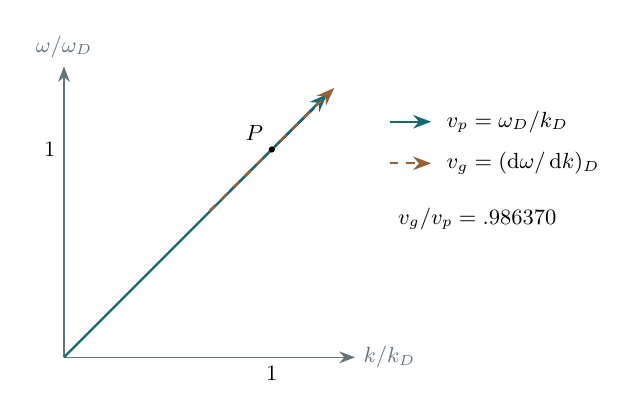
\begin{tikzpicture}[scale=.88,transform shape]
\draw[axis] (0,0)--(4.2,0) node[right] {$k/k_D$};\draw[axis] (0,0)--(0,4.2) node[above] {$\omega/\omega_D$};
\draw[thick,color=ink] plot coordinates {(2.3937945,2.4000000) (2.3988294,2.4050000) (2.4038646,2.4100000) (2.4089001,2.4150000) (2.4139358,2.4200000) (2.4189718,2.4250000) (2.4240081,2.4300000) (2.4290447,2.4350000) (2.4340815,2.4400000) (2.4391186,2.4450000) (2.4441560,2.4500000) (2.4491937,2.4550000) (2.4542316,2.4600000) (2.4592698,2.4650000) (2.4643083,2.4700000) (2.4693471,2.4750000) (2.4743861,2.4800000) (2.4794255,2.4850000) (2.4844651,2.4900000) (2.4895049,2.4950000) (2.4945451,2.5000000) (2.4995855,2.5050000) (2.5046262,2.5100000) (2.5096672,2.5150000) (2.5147085,2.5200000) (2.5197500,2.5250000) (2.5247918,2.5300000) (2.5298339,2.5350000) (2.5348763,2.5400000) (2.5399190,2.5450000) (2.5449619,2.5500000) (2.5500051,2.5550000) (2.5550486,2.5600000) (2.5600924,2.5650000) (2.5651365,2.5700000) (2.5701808,2.5750000) (2.5752255,2.5800000) (2.5802704,2.5850000) (2.5853156,2.5900000) (2.5903610,2.5950000) (2.5954068,2.6000000) (2.6004528,2.6050000) (2.6054992,2.6100000) (2.6105458,2.6150000) (2.6155927,2.6200000) (2.6206398,2.6250000) (2.6256873,2.6300000) (2.6307350,2.6350000) (2.6357831,2.6400000) (2.6408314,2.6450000) (2.6458800,2.6500000) (2.6509288,2.6550000) (2.6559780,2.6600000) (2.6610275,2.6650000) (2.6660772,2.6700000) (2.6711272,2.6750000) (2.6761775,2.6800000) (2.6812281,2.6850000) (2.6862790,2.6900000) (2.6913302,2.6950000) (2.6963816,2.7000000) (2.7014334,2.7050000) (2.7064854,2.7100000) (2.7115377,2.7150000) (2.7165903,2.7200000) (2.7216432,2.7250000) (2.7266964,2.7300000) (2.7317499,2.7350000) (2.7368036,2.7400000) (2.7418577,2.7450000) (2.7469120,2.7500000) (2.7519666,2.7550000) (2.7570215,2.7600000) (2.7620767,2.7650000) (2.7671322,2.7700000) (2.7721880,2.7750000) (2.7772441,2.7800000) (2.7823004,2.7850000) (2.7873571,2.7900000) (2.7924140,2.7950000) (2.7974713,2.8000000) (2.8025288,2.8050000) (2.8075866,2.8100000) (2.8126447,2.8150000) (2.8177031,2.8200000) (2.8227618,2.8250000) (2.8278207,2.8300000) (2.8328800,2.8350000) (2.8379396,2.8400000) (2.8429994,2.8450000) (2.8480595,2.8500000) (2.8531200,2.8550000) (2.8581807,2.8600000) (2.8632417,2.8650000) (2.8683030,2.8700000) (2.8733646,2.8750000) (2.8784265,2.8800000) (2.8834887,2.8850000) (2.8885512,2.8900000) (2.8936140,2.8950000) (2.8986770,2.9000000) (2.9037404,2.9050000) (2.9088040,2.9100000) (2.9138680,2.9150000) (2.9189322,2.9200000) (2.9239967,2.9250000) (2.9290616,2.9300000) (2.9341267,2.9350000) (2.9391921,2.9400000) (2.9442578,2.9450000) (2.9493238,2.9500000) (2.9543901,2.9550000) (2.9594567,2.9600000) (2.9645236,2.9650000) (2.9695908,2.9700000) (2.9746582,2.9750000) (2.9797260,2.9800000) (2.9847940,2.9850000) (2.9898624,2.9900000) (2.9949311,2.9950000) (3.0000000,3.0000000) (3.0050692,3.0050000) (3.0101388,3.0100000) (3.0152086,3.0150000) (3.0202787,3.0200000) (3.0253491,3.0250000) (3.0304199,3.0300000) (3.0354909,3.0350000) (3.0405622,3.0400000) (3.0456338,3.0450000) (3.0507057,3.0500000) (3.0557779,3.0550000) (3.0608504,3.0600000) (3.0659231,3.0650000) (3.0709962,3.0700000) (3.0760696,3.0750000) (3.0811433,3.0800000) (3.0862172,3.0850000) (3.0912915,3.0900000) (3.0963661,3.0950000) (3.1014409,3.1000000) (3.1065161,3.1050000) (3.1115915,3.1100000) (3.1166672,3.1150000) (3.1217433,3.1200000) (3.1268196,3.1250000) (3.1318962,3.1300000) (3.1369732,3.1350000) (3.1420504,3.1400000) (3.1471279,3.1450000) (3.1522057,3.1500000) (3.1572838,3.1550000) (3.1623622,3.1600000) (3.1674409,3.1650000) (3.1725199,3.1700000) (3.1775992,3.1750000) (3.1826788,3.1800000) (3.1877587,3.1850000) (3.1928389,3.1900000) (3.1979194,3.1950000) (3.2030001,3.2000000) (3.2080812,3.2050000) (3.2131626,3.2100000) (3.2182442,3.2150000) (3.2233262,3.2200000) (3.2284084,3.2250000) (3.2334910,3.2300000) (3.2385738,3.2350000) (3.2436570,3.2400000) (3.2487404,3.2450000) (3.2538241,3.2500000) (3.2589082,3.2550000) (3.2639925,3.2600000) (3.2690771,3.2650000) (3.2741620,3.2700000) (3.2792472,3.2750000) (3.2843327,3.2800000) (3.2894185,3.2850000) (3.2945046,3.2900000) (3.2995910,3.2950000) (3.3046777,3.3000000) (3.3097647,3.3050000) (3.3148520,3.3100000) (3.3199395,3.3150000) (3.3250274,3.3200000) (3.3301156,3.3250000) (3.3352040,3.3300000) (3.3402928,3.3350000) (3.3453818,3.3400000) (3.3504712,3.3450000) (3.3555608,3.3500000) (3.3606507,3.3550000) (3.3657410,3.3600000) (3.3708315,3.3650000) (3.3759223,3.3700000) (3.3810134,3.3750000) (3.3861048,3.3800000) (3.3911965,3.3850000) (3.3962885,3.3900000) (3.4013808,3.3950000) (3.4064733,3.4000000) (3.4115662,3.4050000) (3.4166594,3.4100000) (3.4217528,3.4150000) (3.4268466,3.4200000) (3.4319406,3.4250000) (3.4370350,3.4300000) (3.4421296,3.4350000) (3.4472245,3.4400000) (3.4523197,3.4450000) (3.4574152,3.4500000) (3.4625110,3.4550000) (3.4676071,3.4600000) (3.4727035,3.4650000) (3.4778002,3.4700000) (3.4828971,3.4750000) (3.4879944,3.4800000) (3.4930919,3.4850000) (3.4981898,3.4900000) (3.5032879,3.4950000) (3.5083863,3.5000000) (3.5134850,3.5050000) (3.5185840,3.5100000) (3.5236833,3.5150000) (3.5287829,3.5200000) (3.5338828,3.5250000) (3.5389830,3.5300000) (3.5440834,3.5350000) (3.5491841,3.5400000) (3.5542852,3.5450000) (3.5593865,3.5500000) (3.5644881,3.5550000) (3.5695900,3.5600000) (3.5746922,3.5650000) (3.5797947,3.5700000) (3.5848974,3.5750000) (3.5900005,3.5800000) (3.5951038,3.5850000) (3.6002075,3.5900000) (3.6053114,3.5950000) (3.6104156,3.6000000)};
\draw[motion] (0,0)--(3.8,3.8);
\draw[force,dashed] (2.1,2.1122671)--(3.9,3.8877329);
\fill (3,3) circle(.045);\node[above left] at (3,3) {$P$};
\node[below] at (3,0) {$1$};\node[left] at (0,3) {$1$};
\draw[motion] (4.7,3.4)--(5.3,3.4);\node[right,font=\small] at (5.4,3.4) {$v_p=\omega_D/k_D$};
\draw[force,dashed] (4.7,2.8)--(5.3,2.8);\node[right,font=\small] at (5.4,2.8) {$v_g=(\dd\omega/\dd k)_D$};
\node[right,font=\small] at (4.7,2) {$v_g/v_p=.986370$};
\end{tikzpicture}
\figcaption{解图光5.1A\quad 校准玻璃的实际局部色散，原点割线与工作点切线}
\end{minipage}\end{center}
解图光5.1C把两种速度作为波长的函数直接比较。若整条使用未校准的$A,B,C$拟合式，则工作点给$v_p=1.9793794\times10^8\,\mathrm{m/s}$、$v_g=1.9523884\times10^8\,\mathrm{m/s}$；两者相应地采用$n_{\rm fit}$及其群折射率。常数项的校准不改变$n'$，却会同量改变$n$与$n_g$，因而两种速度也随之改变。
\begin{center}\begin{minipage}{.98\linewidth}\centering
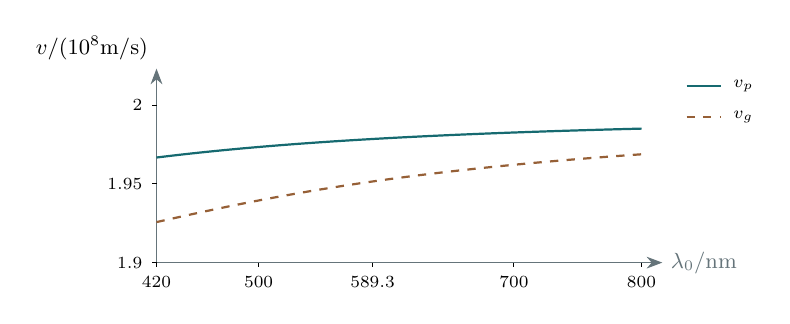
\begin{tikzpicture}[scale=.88,transform shape]
\draw[axis] (0,0)--(7.3,0) node[right] {$\lambda_0/{\rm nm}$};
\draw[axis] (0,0)--(0,2.8);
\node[above left] at (0,2.8) {$v/(10^8{\rm m/s})$};
\draw[thin] (0.000000,0)--(0.000000,-0.06);\node[below,font=\scriptsize] at (0.000000,-0.08) {$ 420 $};
\draw[thin] (1.473684,0)--(1.473684,-0.06);\node[below,font=\scriptsize] at (1.473684,-0.08) {$ 500 $};
\draw[thin] (3.118684,0)--(3.118684,-0.06);\node[below,font=\scriptsize] at (3.118684,-0.08) {$ 589.3 $};
\draw[thin] (5.157895,0)--(5.157895,-0.06);\node[below,font=\scriptsize] at (5.157895,-0.08) {$ 700 $};
\draw[thin] (7.000000,0)--(7.000000,-0.06);\node[below,font=\scriptsize] at (7.000000,-0.08) {$ 800 $};
\draw[thin] (0,0.000000)--(-.06,0.000000);\node[left,font=\scriptsize] at (-.08,0.000000) {$ 1.9 $};
\draw[thin] (0,1.136364)--(-.06,1.136364);\node[left,font=\scriptsize] at (-.08,1.136364) {$ 1.95 $};
\draw[thin] (0,2.272727)--(-.06,2.272727);\node[left,font=\scriptsize] at (-.08,2.272727) {$ 2 $};
\draw[thick,color=accent] plot coordinates {(0.0000000,1.5167512) (0.0291667,1.5203264) (0.0583333,1.5238764) (0.0875000,1.5274015) (0.1166667,1.5309018) (0.1458333,1.5343773) (0.1750000,1.5378283) (0.2041667,1.5412547) (0.2333333,1.5446567) (0.2625000,1.5480345) (0.2916667,1.5513881) (0.3208333,1.5547177) (0.3500000,1.5580235) (0.3791667,1.5613055) (0.4083333,1.5645639) (0.4375000,1.5677988) (0.4666667,1.5710104) (0.4958333,1.5741988) (0.5250000,1.5773641) (0.5541667,1.5805065) (0.5833333,1.5836262) (0.6125000,1.5867232) (0.6416667,1.5897977) (0.6708333,1.5928499) (0.7000000,1.5958799) (0.7291667,1.5988879) (0.7583333,1.6018740) (0.7875000,1.6048383) (0.8166667,1.6077810) (0.8458333,1.6107023) (0.8750000,1.6136023) (0.9041667,1.6164812) (0.9333333,1.6193391) (0.9625000,1.6221761) (0.9916667,1.6249924) (1.0208333,1.6277882) (1.0500000,1.6305636) (1.0791667,1.6333188) (1.1083333,1.6360538) (1.1375000,1.6387690) (1.1666667,1.6414643) (1.1958333,1.6441400) (1.2250000,1.6467962) (1.2541667,1.6494331) (1.2833333,1.6520508) (1.3125000,1.6546494) (1.3416667,1.6572291) (1.3708333,1.6597901) (1.4000000,1.6623325) (1.4291667,1.6648564) (1.4583333,1.6673619) (1.4875000,1.6698494) (1.5166667,1.6723187) (1.5458333,1.6747702) (1.5750000,1.6772040) (1.6041667,1.6796201) (1.6333333,1.6820188) (1.6625000,1.6844002) (1.6916667,1.6867643) (1.7208333,1.6891115) (1.7500000,1.6914417) (1.7791667,1.6937551) (1.8083333,1.6960520) (1.8375000,1.6983323) (1.8666667,1.7005962) (1.8958333,1.7028439) (1.9250000,1.7050756) (1.9541667,1.7072912) (1.9833333,1.7094910) (2.0125000,1.7116751) (2.0416667,1.7138436) (2.0708333,1.7159967) (2.1000000,1.7181344) (2.1291667,1.7202570) (2.1583333,1.7223645) (2.1875000,1.7244570) (2.2166667,1.7265347) (2.2458333,1.7285977) (2.2750000,1.7306461) (2.3041667,1.7326800) (2.3333333,1.7346996) (2.3625000,1.7367050) (2.3916667,1.7386963) (2.4208333,1.7406736) (2.4500000,1.7426370) (2.4791667,1.7445867) (2.5083333,1.7465227) (2.5375000,1.7484452) (2.5666667,1.7503543) (2.5958333,1.7522501) (2.6250000,1.7541327) (2.6541667,1.7560022) (2.6833333,1.7578587) (2.7125000,1.7597024) (2.7416667,1.7615332) (2.7708333,1.7633515) (2.8000000,1.7651572) (2.8291667,1.7669504) (2.8583333,1.7687313) (2.8875000,1.7705000) (2.9166667,1.7722565) (2.9458333,1.7740010) (2.9750000,1.7757335) (3.0041667,1.7774542) (3.0333333,1.7791632) (3.0625000,1.7808605) (3.0916667,1.7825463) (3.1208333,1.7842206) (3.1500000,1.7858836) (3.1791667,1.7875353) (3.2083333,1.7891759) (3.2375000,1.7908053) (3.2666667,1.7924238) (3.2958333,1.7940314) (3.3250000,1.7956282) (3.3541667,1.7972142) (3.3833333,1.7987897) (3.4125000,1.8003546) (3.4416667,1.8019090) (3.4708333,1.8034531) (3.5000000,1.8049869) (3.5291667,1.8065105) (3.5583333,1.8080240) (3.5875000,1.8095274) (3.6166667,1.8110209) (3.6458333,1.8125046) (3.6750000,1.8139784) (3.7041667,1.8154426) (3.7333333,1.8168971) (3.7625000,1.8183421) (3.7916667,1.8197776) (3.8208333,1.8212037) (3.8500000,1.8226205) (3.8791667,1.8240280) (3.9083333,1.8254264) (3.9375000,1.8268157) (3.9666667,1.8281960) (3.9958333,1.8295673) (4.0250000,1.8309297) (4.0541667,1.8322834) (4.0833333,1.8336283) (4.1125000,1.8349646) (4.1416667,1.8362923) (4.1708333,1.8376114) (4.2000000,1.8389221) (4.2291667,1.8402244) (4.2583333,1.8415184) (4.2875000,1.8428042) (4.3166667,1.8440817) (4.3458333,1.8453512) (4.3750000,1.8466126) (4.4041667,1.8478660) (4.4333333,1.8491115) (4.4625000,1.8503491) (4.4916667,1.8515789) (4.5208333,1.8528010) (4.5500000,1.8540154) (4.5791667,1.8552221) (4.6083333,1.8564214) (4.6375000,1.8576131) (4.6666667,1.8587974) (4.6958333,1.8599743) (4.7250000,1.8611439) (4.7541667,1.8623062) (4.7833333,1.8634614) (4.8125000,1.8646093) (4.8416667,1.8657502) (4.8708333,1.8668841) (4.9000000,1.8680109) (4.9291667,1.8691309) (4.9583333,1.8702439) (4.9875000,1.8713502) (5.0166667,1.8724496) (5.0458333,1.8735424) (5.0750000,1.8746285) (5.1041667,1.8757080) (5.1333333,1.8767809) (5.1625000,1.8778473) (5.1916667,1.8789073) (5.2208333,1.8799608) (5.2500000,1.8810080) (5.2791667,1.8820489) (5.3083333,1.8830835) (5.3375000,1.8841119) (5.3666667,1.8851341) (5.3958333,1.8861502) (5.4250000,1.8871602) (5.4541667,1.8881643) (5.4833333,1.8891623) (5.5125000,1.8901544) (5.5416667,1.8911406) (5.5708333,1.8921209) (5.6000000,1.8930955) (5.6291667,1.8940643) (5.6583333,1.8950274) (5.6875000,1.8959848) (5.7166667,1.8969366) (5.7458333,1.8978828) (5.7750000,1.8988234) (5.8041667,1.8997586) (5.8333333,1.9006883) (5.8625000,1.9016126) (5.8916667,1.9025314) (5.9208333,1.9034450) (5.9500000,1.9043533) (5.9791667,1.9052562) (6.0083333,1.9061540) (6.0375000,1.9070466) (6.0666667,1.9079341) (6.0958333,1.9088164) (6.1250000,1.9096937) (6.1541667,1.9105659) (6.1833333,1.9114332) (6.2125000,1.9122954) (6.2416667,1.9131528) (6.2708333,1.9140053) (6.3000000,1.9148529) (6.3291667,1.9156958) (6.3583333,1.9165338) (6.3875000,1.9173671) (6.4166667,1.9181957) (6.4458333,1.9190196) (6.4750000,1.9198389) (6.5041667,1.9206536) (6.5333333,1.9214637) (6.5625000,1.9222692) (6.5916667,1.9230703) (6.6208333,1.9238668) (6.6500000,1.9246590) (6.6791667,1.9254467) (6.7083333,1.9262300) (6.7375000,1.9270090) (6.7666667,1.9277837) (6.7958333,1.9285541) (6.8250000,1.9293202) (6.8541667,1.9300821) (6.8833333,1.9308399) (6.9125000,1.9315934) (6.9416667,1.9323428) (6.9708333,1.9330881) (7.0000000,1.9338294)};
\draw[thick,color=accent] (7.65,2.55)--(8.15,2.55);\node[right,font=\scriptsize] at (8.2,2.55) {$v_p$};
\draw[thick,dashed,color=warm] plot coordinates {(0.0000000,0.5849142) (0.0291667,0.5914558) (0.0583333,0.5979953) (0.0875000,0.6045315) (0.1166667,0.6110631) (0.1458333,0.6175891) (0.1750000,0.6241083) (0.2041667,0.6306198) (0.2333333,0.6371226) (0.2625000,0.6436157) (0.2916667,0.6500981) (0.3208333,0.6565690) (0.3500000,0.6630277) (0.3791667,0.6694732) (0.4083333,0.6759048) (0.4375000,0.6823218) (0.4666667,0.6887234) (0.4958333,0.6951091) (0.5250000,0.7014781) (0.5541667,0.7078299) (0.5833333,0.7141638) (0.6125000,0.7204793) (0.6416667,0.7267759) (0.6708333,0.7330531) (0.7000000,0.7393104) (0.7291667,0.7455473) (0.7583333,0.7517633) (0.7875000,0.7579582) (0.8166667,0.7641314) (0.8458333,0.7702826) (0.8750000,0.7764115) (0.9041667,0.7825176) (0.9333333,0.7886008) (0.9625000,0.7946606) (0.9916667,0.8006968) (1.0208333,0.8067092) (1.0500000,0.8126974) (1.0791667,0.8186613) (1.1083333,0.8246005) (1.1375000,0.8305150) (1.1666667,0.8364045) (1.1958333,0.8422688) (1.2250000,0.8481077) (1.2541667,0.8539211) (1.2833333,0.8597089) (1.3125000,0.8654708) (1.3416667,0.8712068) (1.3708333,0.8769168) (1.4000000,0.8826007) (1.4291667,0.8882582) (1.4583333,0.8938895) (1.4875000,0.8994944) (1.5166667,0.9050727) (1.5458333,0.9106245) (1.5750000,0.9161498) (1.6041667,0.9216484) (1.6333333,0.9271203) (1.6625000,0.9325655) (1.6916667,0.9379840) (1.7208333,0.9433757) (1.7500000,0.9487406) (1.7791667,0.9540788) (1.8083333,0.9593903) (1.8375000,0.9646749) (1.8666667,0.9699328) (1.8958333,0.9751640) (1.9250000,0.9803685) (1.9541667,0.9855463) (1.9833333,0.9906975) (2.0125000,0.9958220) (2.0416667,1.0009199) (2.0708333,1.0059914) (2.1000000,1.0110363) (2.1291667,1.0160548) (2.1583333,1.0210470) (2.1875000,1.0260128) (2.2166667,1.0309524) (2.2458333,1.0358657) (2.2750000,1.0407530) (2.3041667,1.0456142) (2.3333333,1.0504495) (2.3625000,1.0552588) (2.3916667,1.0600424) (2.4208333,1.0648002) (2.4500000,1.0695323) (2.4791667,1.0742389) (2.5083333,1.0789200) (2.5375000,1.0835757) (2.5666667,1.0882062) (2.5958333,1.0928114) (2.6250000,1.0973916) (2.6541667,1.1019467) (2.6833333,1.1064770) (2.7125000,1.1109824) (2.7416667,1.1154631) (2.7708333,1.1199193) (2.8000000,1.1243509) (2.8291667,1.1287582) (2.8583333,1.1331412) (2.8875000,1.1375000) (2.9166667,1.1418348) (2.9458333,1.1461456) (2.9750000,1.1504325) (3.0041667,1.1546958) (3.0333333,1.1589354) (3.0625000,1.1631515) (3.0916667,1.1673443) (3.1208333,1.1715137) (3.1500000,1.1756600) (3.1791667,1.1797833) (3.2083333,1.1838837) (3.2375000,1.1879612) (3.2666667,1.1920160) (3.2958333,1.1960483) (3.3250000,1.2000581) (3.3541667,1.2040456) (3.3833333,1.2080108) (3.4125000,1.2119540) (3.4416667,1.2158751) (3.4708333,1.2197744) (3.5000000,1.2236520) (3.5291667,1.2275079) (3.5583333,1.2313423) (3.5875000,1.2351553) (3.6166667,1.2389470) (3.6458333,1.2427176) (3.6750000,1.2464672) (3.7041667,1.2501958) (3.7333333,1.2539037) (3.7625000,1.2575908) (3.7916667,1.2612574) (3.8208333,1.2649036) (3.8500000,1.2685294) (3.8791667,1.2721350) (3.9083333,1.2757205) (3.9375000,1.2792861) (3.9666667,1.2828318) (3.9958333,1.2863577) (4.0250000,1.2898641) (4.0541667,1.2933509) (4.0833333,1.2968183) (4.1125000,1.3002665) (4.1416667,1.3036955) (4.1708333,1.3071054) (4.2000000,1.3104964) (4.2291667,1.3138686) (4.2583333,1.3172221) (4.2875000,1.3205570) (4.3166667,1.3238734) (4.3458333,1.3271715) (4.3750000,1.3304513) (4.4041667,1.3337129) (4.4333333,1.3369565) (4.4625000,1.3401822) (4.4916667,1.3433901) (4.5208333,1.3465802) (4.5500000,1.3497528) (4.5791667,1.3529079) (4.6083333,1.3560456) (4.6375000,1.3591660) (4.6666667,1.3622693) (4.6958333,1.3653555) (4.7250000,1.3684247) (4.7541667,1.3714772) (4.7833333,1.3745128) (4.8125000,1.3775319) (4.8416667,1.3805343) (4.8708333,1.3835204) (4.9000000,1.3864901) (4.9291667,1.3894437) (4.9583333,1.3923810) (4.9875000,1.3953024) (5.0166667,1.3982079) (5.0458333,1.4010975) (5.0750000,1.4039714) (5.1041667,1.4068297) (5.1333333,1.4096724) (5.1625000,1.4124997) (5.1916667,1.4153117) (5.2208333,1.4181085) (5.2500000,1.4208901) (5.2791667,1.4236567) (5.3083333,1.4264084) (5.3375000,1.4291452) (5.3666667,1.4318672) (5.3958333,1.4345746) (5.4250000,1.4372674) (5.4541667,1.4399457) (5.4833333,1.4426096) (5.5125000,1.4452593) (5.5416667,1.4478947) (5.5708333,1.4505160) (5.6000000,1.4531233) (5.6291667,1.4557167) (5.6583333,1.4582962) (5.6875000,1.4608620) (5.7166667,1.4634141) (5.7458333,1.4659526) (5.7750000,1.4684776) (5.8041667,1.4709892) (5.8333333,1.4734874) (5.8625000,1.4759725) (5.8916667,1.4784443) (5.9208333,1.4809031) (5.9500000,1.4833489) (5.9791667,1.4857818) (6.0083333,1.4882019) (6.0375000,1.4906092) (6.0666667,1.4930038) (6.0958333,1.4953859) (6.1250000,1.4977554) (6.1541667,1.5001126) (6.1833333,1.5024574) (6.2125000,1.5047899) (6.2416667,1.5071102) (6.2708333,1.5094184) (6.3000000,1.5117146) (6.3291667,1.5139988) (6.3583333,1.5162712) (6.3875000,1.5185317) (6.4166667,1.5207805) (6.4458333,1.5230176) (6.4750000,1.5252432) (6.5041667,1.5274572) (6.5333333,1.5296598) (6.5625000,1.5318510) (6.5916667,1.5340310) (6.6208333,1.5361997) (6.6500000,1.5383572) (6.6791667,1.5405037) (6.7083333,1.5426392) (6.7375000,1.5447637) (6.7666667,1.5468773) (6.7958333,1.5489801) (6.8250000,1.5510722) (6.8541667,1.5531536) (6.8833333,1.5552244) (6.9125000,1.5572847) (6.9416667,1.5593345) (6.9708333,1.5613739) (7.0000000,1.5634030)};
\draw[thick,dashed,color=warm] (7.65,2.0999999999999996)--(8.15,2.0999999999999996);\node[right,font=\scriptsize] at (8.2,2.0999999999999996) {$v_g$};
\end{tikzpicture}
\figcaption{解图光5.1C\quad 可见光局部模型中群速低于相速}
\end{minipage}\end{center}
弱色散的一次近似由同一分母展开得到。令$\eta=\lambda_0n'/n=-.01381846$，则
\[
v_g=\frac cn\frac1{1-\eta}
=\frac cn(1+\eta+O(\eta^2)).
\]
一次式给$v_g^{(1)}=1.9511605\times10^8\,\mathrm{m/s}$，精确群速关系给$1.9515331\times10^8\,\mathrm{m/s}$。两者相对差为
\[
 \frac{v_g-v_g^{(1)}}{v_g}
 =1-(1+\eta)(1-\eta)=\eta^2=.000190950=0.0190950\%.
\]
解图光5.1D显示这一误差随波长变化，纵轴以百分数表示$\eta^2$。
\begin{center}\begin{minipage}{.98\linewidth}\centering
\begin{tikzpicture}[scale=.88,transform shape]
\draw[axis] (0,0.0)--(7.3,0.0) node[right] {$\lambda_0/{\rm nm}$};
\draw[axis] (0,0)--(0,2.8);
\node[above left] at (0,2.8) {$\text{相对差}/\%$};
\draw[thin] (0.000000,0.0)--(0.000000,-0.06);\node[below,font=\scriptsize] at (0.000000,-0.08) {$ 420 $};
\draw[thin] (1.473684,0.0)--(1.473684,-0.06);\node[below,font=\scriptsize] at (1.473684,-0.08) {$ 500 $};
\draw[thin] (3.118684,0.0)--(3.118684,-0.06);\node[below,font=\scriptsize] at (3.118684,-0.08) {$ 589.3 $};
\draw[thin] (5.157895,0.0)--(5.157895,-0.06);\node[below,font=\scriptsize] at (5.157895,-0.08) {$ 700 $};
\draw[thin] (7.000000,0.0)--(7.000000,-0.06);\node[below,font=\scriptsize] at (7.000000,-0.08) {$ 800 $};
\draw[thin] (0,0.000000)--(-.06,0.000000);\node[left,font=\scriptsize] at (-.08,0.000000) {$ 0 $};
\draw[thin] (0,0.833333)--(-.06,0.833333);\node[left,font=\scriptsize] at (-.08,0.833333) {$ 0.02 $};
\draw[thin] (0,1.666667)--(-.06,1.666667);\node[left,font=\scriptsize] at (-.08,1.666667) {$ 0.04 $};
\draw[thin] (0,2.500000)--(-.06,2.500000);\node[left,font=\scriptsize] at (-.08,2.500000) {$ 0.06 $};
\draw[thick,color=accent] plot coordinates {(0.0000000,1.8887759) (0.0291667,1.8762083) (0.0583333,1.8635944) (0.0875000,1.8509403) (0.1166667,1.8382522) (0.1458333,1.8255359) (0.1750000,1.8127971) (0.2041667,1.8000412) (0.2333333,1.7872731) (0.2625000,1.7744979) (0.2916667,1.7617203) (0.3208333,1.7489448) (0.3500000,1.7361757) (0.3791667,1.7234171) (0.4083333,1.7106730) (0.4375000,1.6979470) (0.4666667,1.6852429) (0.4958333,1.6725639) (0.5250000,1.6599135) (0.5541667,1.6472946) (0.5833333,1.6347103) (0.6125000,1.6221633) (0.6416667,1.6096564) (0.6708333,1.5971921) (0.7000000,1.5847728) (0.7291667,1.5724009) (0.7583333,1.5600784) (0.7875000,1.5478075) (0.8166667,1.5355901) (0.8458333,1.5234280) (0.8750000,1.5113231) (0.9041667,1.4992770) (0.9333333,1.4872912) (0.9625000,1.4753671) (0.9916667,1.4635063) (1.0208333,1.4517099) (1.0500000,1.4399792) (1.0791667,1.4283153) (1.1083333,1.4167192) (1.1375000,1.4051920) (1.1666667,1.3937347) (1.1958333,1.3823479) (1.2250000,1.3710326) (1.2541667,1.3597894) (1.2833333,1.3486191) (1.3125000,1.3375222) (1.3416667,1.3264993) (1.3708333,1.3155509) (1.4000000,1.3046775) (1.4291667,1.2938795) (1.4583333,1.2831572) (1.4875000,1.2725110) (1.5166667,1.2619412) (1.5458333,1.2514479) (1.5750000,1.2410314) (1.6041667,1.2306919) (1.6333333,1.2204295) (1.6625000,1.2102443) (1.6916667,1.2001363) (1.7208333,1.1901055) (1.7500000,1.1801521) (1.7791667,1.1702759) (1.8083333,1.1604769) (1.8375000,1.1507550) (1.8666667,1.1411102) (1.8958333,1.1315422) (1.9250000,1.1220510) (1.9541667,1.1126363) (1.9833333,1.1032980) (2.0125000,1.0940359) (2.0416667,1.0848498) (2.0708333,1.0757393) (2.1000000,1.0667043) (2.1291667,1.0577444) (2.1583333,1.0488594) (2.1875000,1.0400489) (2.2166667,1.0313127) (2.2458333,1.0226504) (2.2750000,1.0140616) (2.3041667,1.0055461) (2.3333333,0.9971034) (2.3625000,0.9887331) (2.3916667,0.9804349) (2.4208333,0.9722084) (2.4500000,0.9640532) (2.4791667,0.9559688) (2.5083333,0.9479548) (2.5375000,0.9400109) (2.5666667,0.9321366) (2.5958333,0.9243314) (2.6250000,0.9165949) (2.6541667,0.9089266) (2.6833333,0.9013262) (2.7125000,0.8937931) (2.7416667,0.8863269) (2.7708333,0.8789270) (2.8000000,0.8715932) (2.8291667,0.8643248) (2.8583333,0.8571214) (2.8875000,0.8499825) (2.9166667,0.8429077) (2.9458333,0.8358964) (2.9750000,0.8289483) (3.0041667,0.8220627) (3.0333333,0.8152392) (3.0625000,0.8084774) (3.0916667,0.8017767) (3.1208333,0.7951367) (3.1500000,0.7885568) (3.1791667,0.7820367) (3.2083333,0.7755757) (3.2375000,0.7691735) (3.2666667,0.7628295) (3.2958333,0.7565432) (3.3250000,0.7503142) (3.3541667,0.7441420) (3.3833333,0.7380261) (3.4125000,0.7319660) (3.4416667,0.7259612) (3.4708333,0.7200113) (3.5000000,0.7141158) (3.5291667,0.7082742) (3.5583333,0.7024861) (3.5875000,0.6967509) (3.6166667,0.6910683) (3.6458333,0.6854376) (3.6750000,0.6798586) (3.7041667,0.6743307) (3.7333333,0.6688534) (3.7625000,0.6634263) (3.7916667,0.6580490) (3.8208333,0.6527210) (3.8500000,0.6474418) (3.8791667,0.6422110) (3.9083333,0.6370282) (3.9375000,0.6318929) (3.9666667,0.6268046) (3.9958333,0.6217630) (4.0250000,0.6167676) (4.0541667,0.6118180) (4.0833333,0.6069138) (4.1125000,0.6020544) (4.1416667,0.5972396) (4.1708333,0.5924688) (4.2000000,0.5877418) (4.2291667,0.5830580) (4.2583333,0.5784170) (4.2875000,0.5738185) (4.3166667,0.5692620) (4.3458333,0.5647472) (4.3750000,0.5602736) (4.4041667,0.5558409) (4.4333333,0.5514487) (4.4625000,0.5470965) (4.4916667,0.5427840) (4.5208333,0.5385109) (4.5500000,0.5342766) (4.5791667,0.5300810) (4.6083333,0.5259235) (4.6375000,0.5218038) (4.6666667,0.5177216) (4.6958333,0.5136765) (4.7250000,0.5096682) (4.7541667,0.5056962) (4.7833333,0.5017602) (4.8125000,0.4978599) (4.8416667,0.4939950) (4.8708333,0.4901650) (4.9000000,0.4863697) (4.9291667,0.4826087) (4.9583333,0.4788817) (4.9875000,0.4751883) (5.0166667,0.4715283) (5.0458333,0.4679012) (5.0750000,0.4643068) (5.1041667,0.4607448) (5.1333333,0.4572148) (5.1625000,0.4537165) (5.1916667,0.4502497) (5.2208333,0.4468139) (5.2500000,0.4434090) (5.2791667,0.4400345) (5.3083333,0.4366903) (5.3375000,0.4333760) (5.3666667,0.4300912) (5.3958333,0.4268358) (5.4250000,0.4236095) (5.4541667,0.4204119) (5.4833333,0.4172428) (5.5125000,0.4141018) (5.5416667,0.4109888) (5.5708333,0.4079034) (5.6000000,0.4048454) (5.6291667,0.4018145) (5.6583333,0.3988104) (5.6875000,0.3958330) (5.7166667,0.3928818) (5.7458333,0.3899567) (5.7750000,0.3870574) (5.8041667,0.3841836) (5.8333333,0.3813352) (5.8625000,0.3785118) (5.8916667,0.3757132) (5.9208333,0.3729391) (5.9500000,0.3701894) (5.9791667,0.3674638) (6.0083333,0.3647620) (6.0375000,0.3620839) (6.0666667,0.3594291) (6.0958333,0.3567975) (6.1250000,0.3541889) (6.1541667,0.3516029) (6.1833333,0.3490394) (6.2125000,0.3464982) (6.2416667,0.3439791) (6.2708333,0.3414818) (6.3000000,0.3390061) (6.3291667,0.3365519) (6.3583333,0.3341188) (6.3875000,0.3317067) (6.4166667,0.3293155) (6.4458333,0.3269448) (6.4750000,0.3245945) (6.5041667,0.3222645) (6.5333333,0.3199544) (6.5625000,0.3176641) (6.5916667,0.3153935) (6.6208333,0.3131423) (6.6500000,0.3109103) (6.6791667,0.3086973) (6.7083333,0.3065033) (6.7375000,0.3043279) (6.7666667,0.3021710) (6.7958333,0.3000325) (6.8250000,0.2979121) (6.8541667,0.2958097) (6.8833333,0.2937251) (6.9125000,0.2916581) (6.9416667,0.2896086) (6.9708333,0.2875763) (7.0000000,0.2855612)};
\end{tikzpicture}
\figcaption{解图光5.1D\quad 弱色散一次式低于完整分母结果，相对差等于$\eta^2$}
\end{minipage}\end{center}
介质内波长形式的Rayleigh关系也可由链式求导得到。由$\lambda_m=\lambda_0/n$，
\[
 \frac{\dd\lambda_m}{\dd\lambda_0}=\frac{n_g}{n^2},\qquad
 \frac{\dd v_p}{\dd\lambda_m}=-\frac{c n'}{n_g},\qquad
 v_p-\lambda_m\frac{\dd v_p}{\dd\lambda_m}=\frac c{n_g}.
\]
这个严格表达中的自变量是$\lambda_m$；以真空波长$\lambda_0$展开时则回到前面的群折射率分母。群速描述中心频率附近的一次相位差传播，透明窄带条件下也对应能量包络的传播。带宽扩大后，$k''=\dd^2k/\dd\omega^2$产生频率相关的群延迟，包络还会展宽，传播时需同时保留这一二阶项。


\Needspace{13\baselineskip}

\pdfbookmark[2]{第 2 题 氢气的有效共振与振子参数}{q2}

\section*{第 2 题\quad 氢气的有效共振与振子参数}\label{q:2}

常温常压下，氢气在$0.4$至$9\,\mu\mathrm m$波段满足
\[
n^2=1+a+\frac b{\lambda_0^2},\qquad a=2.721\times10^{-4},\quad b=2.11\times10^{-18}\,\mathrm{m^2},
\]
电子吸收带位于远紫外，密度为$9.0\times10^{-2}\,\mathrm{kg/m^3}$。用单振子、弱极化模型估算有效本征频率及共振真空波长；再求振子的荷质比。讨论荷质比的确定需要什么电荷及数密度假设，取氢原子摩尔质量$1.0\times10^{-3}\,\mathrm{kg/mol}$。

\begin{center}\begin{minipage}{.98\linewidth}\centering
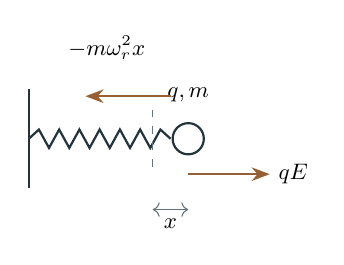
\begin{tikzpicture}[scale=.9,transform shape]
\draw[object] (0.00000,-0.70000)--(0.00000,0.70000);\draw[object] plot coordinates {(0.00000,0.00000) (0.14286,0.13000) (0.28571,-0.13000) (0.42857,0.13000) (0.57143,-0.13000) (0.71429,0.13000) (0.85714,-0.13000) (1.00000,0.13000) (1.14286,-0.13000) (1.28571,0.13000) (1.42857,-0.13000) (1.57143,0.13000) (1.71429,-0.13000) (1.85714,0.13000) (2.00000,0.00000)};\draw[object] (2.25000,0.00000) circle(0.22000);\node[above] at (2.25000,0.40000) {$q,m$};\draw[force] (2.25000,-0.50000)--(3.40000,-0.50000);\node[right] at (3.40000,-0.50000) {$qE$};\draw[force] (2.00000,0.60000)--(0.80000,0.60000);\node[above] at (1.10000,1.00000) {$-m\omega_r^2x$};\draw[<->,thin,color=muted] (1.75000,-1.00000)--(2.25000,-1.00000);\node[below] at (2.00000,-1.00000) {$x$};\draw[guide] (1.75000,-0.40000)--(1.75000,0.40000);
\end{tikzpicture}
\figcaption{图光5.2\quad 束缚振子的外力、回复力与位移。}
\end{minipage}\end{center}

\Needspace{6\baselineskip}\subsection*{解答}


图光5.2中，电荷$q$相对平衡点的位移为$x$，外力为$qE$，回复力为$-m\omega_r^2x$。在远离吸收带的稀薄气体中，用单个有效共振代表该波段的束缚电子响应，先忽略阻尼。取$e^{-i\omega t}$，振动方程及偶极极化为
\[
m\ddot x+m\omega_r^2x=qE,\qquad
x=\frac{qE}{m(\omega_r^2-\omega^2)},\qquad
P=Nqx.
\]
若有多类振子，一般响应为$ n^2-1=(N/\varepsilon_0)\sum_jf_jq_j^2/[m_j(\omega_j^2-\omega^2)]$，$f_j$给各类权重。当前采用一类有效参数，并取局部场近似为宏观场，$P=\varepsilon_0(n^2-1)E$，便得到
\[
n^2-1=\frac{Nq^2}{\varepsilon_0m(\omega_r^2-\omega^2)}
=\frac{Nq^2}{4\pi^2\varepsilon_0m(\nu_r^2-\nu^2)}.
\]
其中$\omega_r=2\pi\nu_r$，从角频率改写成普通频率带来$4\pi^2$因子。令$x_\nu=\nu^2/\nu_r^2=(\lambda_r/\lambda_0)^2$，长波区$0<x_\nu\ll1$有$(1-x_\nu)^{-1}=1+x_\nu+O(x_\nu^2)$，因此
\[
n^2-1\simeq\frac{Nq^2}{4\pi^2\varepsilon_0m\nu_r^2}\left(1+\frac{\nu^2}{\nu_r^2}\right)=\frac{Nq^2}{4\pi^2\varepsilon_0m\nu_r^2}\left(1+\frac{c^2}{\nu_r^2\lambda_0^2}\right).
\]
与题给$n^2-1=a+b/\lambda_0^2$的常数、平方反波长两项分别比较，得
\[
a=\frac{Nq^2}{4\pi^2\varepsilon_0m\nu_r^2},\qquad
b=\frac{ac^2}{\nu_r^2}=a\lambda_r^2.
\]
所以$b/a$直接给共振波长的平方，振子数、电荷与质量在这个比值中消去。解图光5.2A在同一对数波长轴上标出测量窗口与有效共振，二者的距离对应长波展开的尺度。
\begin{center}\begin{minipage}{.98\linewidth}\centering
\begin{tikzpicture}[scale=.9,transform shape]
\draw[axis] (0.00000,0.00000)--(8.50000,0.00000);\node[below right] at (8.50000,0.00000) {$\log\lambda_0$};\draw[force] (0.63863,-0.10000)--(0.63863,1.10000);\node[above] at (0.63863,1.15000) {$\lambda_r=88.06\,\mathrm{nm}$};\draw[very thick,color=accent] (2.34631,0.38000)--(5.85941,0.38000);\draw[<->,thin,color=muted] (2.34631,-0.45000)--(5.85941,-0.45000);\node[below] at (4.10286,-0.45000) {测量波段};\node[above] at (4.00000,1.90000) {长波测量推得的有效共振};
\end{tikzpicture}
\figcaption{解图光5.2A\quad 共振位于测量波段之外；粗线为0.4至9微米。}
\end{minipage}\end{center}
代入$a=2.721\times10^{-4}$、$b=2.11\times10^{-18}\,\mathrm{m^2}$，有
\[
\boxed{\lambda_r=\sqrt{b/a}=8.8060\times10^{-8}\,\mathrm m=88.06\,\mathrm{nm}},
\quad
\boxed{\nu_r=c\sqrt{a/b}=3.407\times10^{15}\,\mathrm{Hz}}.
\]
用未取整的系数得到$\lambda_r=88.05965\,\mathrm{nm}$，按题设精度记约88.1nm。解图光5.2B在测量窗口的短波端比较完整单振子响应$a/(1-x_\nu)$与两项式$a(1+x_\nu)$，显示下一阶项的量级。
\begin{center}\begin{minipage}{.98\linewidth}\centering
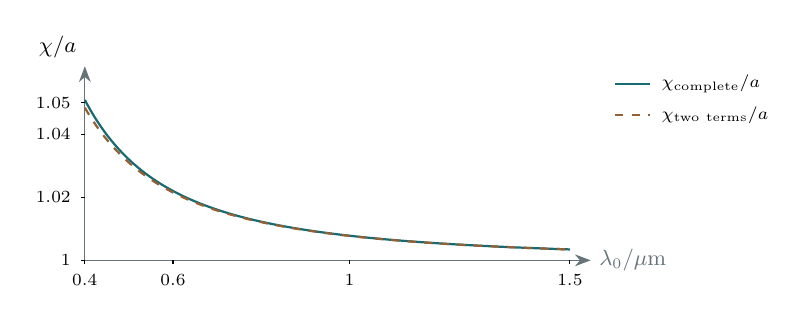
\begin{tikzpicture}[scale=.88,transform shape]
\draw[axis] (0,0)--(7.3,0) node[right] {$\lambda_0/{\rm \mu m}$};
\draw[axis] (0,0)--(0,2.8);
\node[above left] at (0,2.8) {$\chi/a$};
\draw[thin] (0.000000,0)--(0.000000,-0.06);\node[below,font=\scriptsize] at (0.000000,-0.08) {$ 0.4 $};
\draw[thin] (1.272727,0)--(1.272727,-0.06);\node[below,font=\scriptsize] at (1.272727,-0.08) {$ 0.6 $};
\draw[thin] (3.818182,0)--(3.818182,-0.06);\node[below,font=\scriptsize] at (3.818182,-0.08) {$ 1 $};
\draw[thin] (7.000000,0)--(7.000000,-0.06);\node[below,font=\scriptsize] at (7.000000,-0.08) {$ 1.5 $};
\draw[thin] (0,0.000000)--(-.06,0.000000);\node[left,font=\scriptsize] at (-.08,0.000000) {$ 1 $};
\draw[thin] (0,0.909091)--(-.06,0.909091);\node[left,font=\scriptsize] at (-.08,0.909091) {$ 1.02 $};
\draw[thin] (0,1.818182)--(-.06,1.818182);\node[left,font=\scriptsize] at (-.08,1.818182) {$ 1.04 $};
\draw[thin] (0,2.272727)--(-.06,2.272727);\node[left,font=\scriptsize] at (-.08,2.272727) {$ 1.05 $};
\draw[thick,color=accent] plot coordinates {(0.0000000,2.3151907) (0.0291667,2.2604386) (0.0583333,2.2076353) (0.0875000,2.1566881) (0.1166667,2.1075097) (0.1458333,2.0600182) (0.1750000,2.0141363) (0.2041667,1.9697910) (0.2333333,1.9269137) (0.2625000,1.8854395) (0.2916667,1.8453070) (0.3208333,1.8064583) (0.3500000,1.7688387) (0.3791667,1.7323961) (0.4083333,1.6970815) (0.4375000,1.6628482) (0.4666667,1.6296521) (0.4958333,1.5974513) (0.5250000,1.5662059) (0.5541667,1.5358781) (0.5833333,1.5064319) (0.6125000,1.4778333) (0.6416667,1.4500496) (0.6708333,1.4230499) (0.7000000,1.3968046) (0.7291667,1.3712858) (0.7583333,1.3464665) (0.7875000,1.3223212) (0.8166667,1.2988255) (0.8458333,1.2759562) (0.8750000,1.2536908) (0.9041667,1.2320083) (0.9333333,1.2108882) (0.9625000,1.1903111) (0.9916667,1.1702584) (1.0208333,1.1507123) (1.0500000,1.1316557) (1.0791667,1.1130723) (1.1083333,1.0949465) (1.1375000,1.0772632) (1.1666667,1.0600081) (1.1958333,1.0431673) (1.2250000,1.0267276) (1.2541667,1.0106762) (1.2833333,0.9950009) (1.3125000,0.9796901) (1.3416667,0.9647323) (1.3708333,0.9501169) (1.4000000,0.9358332) (1.4291667,0.9218714) (1.4583333,0.9082217) (1.4875000,0.8948748) (1.5166667,0.8818218) (1.5458333,0.8690542) (1.5750000,0.8565635) (1.6041667,0.8443418) (1.6333333,0.8323813) (1.6625000,0.8206747) (1.6916667,0.8092147) (1.7208333,0.7979945) (1.7500000,0.7870073) (1.7791667,0.7762468) (1.8083333,0.7657066) (1.8375000,0.7553808) (1.8666667,0.7452636) (1.8958333,0.7353494) (1.9250000,0.7256327) (1.9541667,0.7161083) (1.9833333,0.7067712) (2.0125000,0.6976164) (2.0416667,0.6886392) (2.0708333,0.6798350) (2.1000000,0.6711994) (2.1291667,0.6627281) (2.1583333,0.6544169) (2.1875000,0.6462618) (2.2166667,0.6382589) (2.2458333,0.6304044) (2.2750000,0.6226946) (2.3041667,0.6151260) (2.3333333,0.6076952) (2.3625000,0.6003988) (2.3916667,0.5932336) (2.4208333,0.5861964) (2.4500000,0.5792842) (2.4791667,0.5724941) (2.5083333,0.5658231) (2.5375000,0.5592686) (2.5666667,0.5528277) (2.5958333,0.5464979) (2.6250000,0.5402765) (2.6541667,0.5341613) (2.6833333,0.5281497) (2.7125000,0.5222393) (2.7416667,0.5164280) (2.7708333,0.5107135) (2.8000000,0.5050937) (2.8291667,0.4995665) (2.8583333,0.4941298) (2.8875000,0.4887817) (2.9166667,0.4835202) (2.9458333,0.4783436) (2.9750000,0.4732499) (3.0041667,0.4682374) (3.0333333,0.4633044) (3.0625000,0.4584493) (3.0916667,0.4536702) (3.1208333,0.4489658) (3.1500000,0.4443344) (3.1791667,0.4397745) (3.2083333,0.4352847) (3.2375000,0.4308635) (3.2666667,0.4265095) (3.2958333,0.4222214) (3.3250000,0.4179978) (3.3541667,0.4138375) (3.3833333,0.4097391) (3.4125000,0.4057015) (3.4416667,0.4017235) (3.4708333,0.3978039) (3.5000000,0.3939415) (3.5291667,0.3901352) (3.5583333,0.3863840) (3.5875000,0.3826868) (3.6166667,0.3790426) (3.6458333,0.3754503) (3.6750000,0.3719090) (3.7041667,0.3684176) (3.7333333,0.3649754) (3.7625000,0.3615812) (3.7916667,0.3582344) (3.8208333,0.3549339) (3.8500000,0.3516789) (3.8791667,0.3484686) (3.9083333,0.3453021) (3.9375000,0.3421788) (3.9666667,0.3390977) (3.9958333,0.3360582) (4.0250000,0.3330594) (4.0541667,0.3301007) (4.0833333,0.3271814) (4.1125000,0.3243006) (4.1416667,0.3214579) (4.1708333,0.3186525) (4.2000000,0.3158837) (4.2291667,0.3131509) (4.2583333,0.3104535) (4.2875000,0.3077909) (4.3166667,0.3051625) (4.3458333,0.3025676) (4.3750000,0.3000058) (4.4041667,0.2974765) (4.4333333,0.2949791) (4.4625000,0.2925130) (4.4916667,0.2900779) (4.5208333,0.2876731) (4.5500000,0.2852981) (4.5791667,0.2829525) (4.6083333,0.2806357) (4.6375000,0.2783473) (4.6666667,0.2760869) (4.6958333,0.2738539) (4.7250000,0.2716480) (4.7541667,0.2694687) (4.7833333,0.2673155) (4.8125000,0.2651881) (4.8416667,0.2630861) (4.8708333,0.2610090) (4.9000000,0.2589564) (4.9291667,0.2569280) (4.9583333,0.2549234) (4.9875000,0.2529422) (5.0166667,0.2509840) (5.0458333,0.2490486) (5.0750000,0.2471354) (5.1041667,0.2452443) (5.1333333,0.2433749) (5.1625000,0.2415267) (5.1916667,0.2396996) (5.2208333,0.2378932) (5.2500000,0.2361071) (5.2791667,0.2343411) (5.3083333,0.2325949) (5.3375000,0.2308682) (5.3666667,0.2291607) (5.3958333,0.2274720) (5.4250000,0.2258020) (5.4541667,0.2241504) (5.4833333,0.2225168) (5.5125000,0.2209011) (5.5416667,0.2193029) (5.5708333,0.2177220) (5.6000000,0.2161582) (5.6291667,0.2146112) (5.6583333,0.2130807) (5.6875000,0.2115667) (5.7166667,0.2100687) (5.7458333,0.2085866) (5.7750000,0.2071201) (5.8041667,0.2056691) (5.8333333,0.2042333) (5.8625000,0.2028125) (5.8916667,0.2014065) (5.9208333,0.2000151) (5.9500000,0.1986381) (5.9791667,0.1972752) (6.0083333,0.1959264) (6.0375000,0.1945914) (6.0666667,0.1932700) (6.0958333,0.1919620) (6.1250000,0.1906673) (6.1541667,0.1893856) (6.1833333,0.1881169) (6.2125000,0.1868608) (6.2416667,0.1856174) (6.2708333,0.1843863) (6.3000000,0.1831674) (6.3291667,0.1819606) (6.3583333,0.1807657) (6.3875000,0.1795825) (6.4166667,0.1784110) (6.4458333,0.1772509) (6.4750000,0.1761020) (6.5041667,0.1749644) (6.5333333,0.1738377) (6.5625000,0.1727219) (6.5916667,0.1716168) (6.6208333,0.1705223) (6.6500000,0.1694382) (6.6791667,0.1683645) (6.7083333,0.1673009) (6.7375000,0.1662475) (6.7666667,0.1652039) (6.7958333,0.1641701) (6.8250000,0.1631461) (6.8541667,0.1621316) (6.8833333,0.1611265) (6.9125000,0.1601308) (6.9416667,0.1591442) (6.9708333,0.1581668) (7.0000000,0.1571984)};
\draw[thick,color=accent] (7.65,2.55)--(8.15,2.55);\node[right,font=\scriptsize] at (8.2,2.55) {$\chi_{\rm complete}/a$};
\draw[thick,dashed,color=warm] plot coordinates {(0.0000000,2.2029835) (0.0291667,2.1533531) (0.0583333,2.1053812) (0.0875000,2.0589947) (0.1166667,2.0141244) (0.1458333,1.9707051) (0.1750000,1.9286747) (0.2041667,1.8879748) (0.2333333,1.8485498) (0.2625000,1.8103469) (0.2916667,1.7733161) (0.3208333,1.7374100) (0.3500000,1.7025836) (0.3791667,1.6687939) (0.4083333,1.6360001) (0.4375000,1.6041637) (0.4666667,1.5732475) (0.4958333,1.5432166) (0.5250000,1.5140374) (0.5541667,1.4856780) (0.5833333,1.4581080) (0.6125000,1.4312984) (0.6416667,1.4052215) (0.6708333,1.3798508) (0.7000000,1.3551610) (0.7291667,1.3311279) (0.7583333,1.3077286) (0.7875000,1.2849409) (0.8166667,1.2627437) (0.8458333,1.2411167) (0.8750000,1.2200406) (0.9041667,1.1994969) (0.9333333,1.1794677) (0.9625000,1.1599360) (0.9916667,1.1408855) (1.0208333,1.1223005) (1.0500000,1.1041659) (1.0791667,1.0864674) (1.1083333,1.0691910) (1.1375000,1.0523234) (1.1666667,1.0358518) (1.1958333,1.0197640) (1.2250000,1.0040481) (1.2541667,0.9886927) (1.2833333,0.9736869) (1.3125000,0.9590201) (1.3416667,0.9446823) (1.3708333,0.9306636) (1.4000000,0.9169546) (1.4291667,0.9035464) (1.4583333,0.8904301) (1.4875000,0.8775973) (1.5166667,0.8650400) (1.5458333,0.8527503) (1.5750000,0.8407206) (1.6041667,0.8289437) (1.6333333,0.8174125) (1.6625000,0.8061203) (1.6916667,0.7950605) (1.7208333,0.7842267) (1.7500000,0.7736129) (1.7791667,0.7632131) (1.8083333,0.7530216) (1.8375000,0.7430328) (1.8666667,0.7332416) (1.8958333,0.7236425) (1.9250000,0.7142308) (1.9541667,0.7050015) (1.9833333,0.6959499) (2.0125000,0.6870715) (2.0416667,0.6783620) (2.0708333,0.6698170) (2.1000000,0.6614325) (2.1291667,0.6532044) (2.1583333,0.6451289) (2.1875000,0.6372022) (2.2166667,0.6294207) (2.2458333,0.6217809) (2.2750000,0.6142794) (2.3041667,0.6069128) (2.3333333,0.5996779) (2.3625000,0.5925717) (2.3916667,0.5855910) (2.4208333,0.5787329) (2.4500000,0.5719946) (2.4791667,0.5653733) (2.5083333,0.5588663) (2.5375000,0.5524710) (2.5666667,0.5461849) (2.5958333,0.5400054) (2.6250000,0.5339302) (2.6541667,0.5279570) (2.6833333,0.5220834) (2.7125000,0.5163073) (2.7416667,0.5106266) (2.7708333,0.5050391) (2.8000000,0.4995428) (2.8291667,0.4941357) (2.8583333,0.4888159) (2.8875000,0.4835816) (2.9166667,0.4784310) (2.9458333,0.4733621) (2.9750000,0.4683734) (3.0041667,0.4634632) (3.0333333,0.4586298) (3.0625000,0.4538716) (3.0916667,0.4491870) (3.1208333,0.4445746) (3.1500000,0.4400329) (3.1791667,0.4355604) (3.2083333,0.4311558) (3.2375000,0.4268177) (3.2666667,0.4225447) (3.2958333,0.4183355) (3.3250000,0.4141889) (3.3541667,0.4101037) (3.3833333,0.4060786) (3.4125000,0.4021125) (3.4416667,0.3982042) (3.4708333,0.3943526) (3.5000000,0.3905566) (3.5291667,0.3868152) (3.5583333,0.3831273) (3.5875000,0.3794918) (3.6166667,0.3759079) (3.6458333,0.3723745) (3.6750000,0.3688907) (3.7041667,0.3654555) (3.7333333,0.3620681) (3.7625000,0.3587276) (3.7916667,0.3554331) (3.8208333,0.3521838) (3.8500000,0.3489789) (3.8791667,0.3458174) (3.9083333,0.3426988) (3.9375000,0.3396221) (3.9666667,0.3365867) (3.9958333,0.3335918) (4.0250000,0.3306367) (4.0541667,0.3277207) (4.0833333,0.3248431) (4.1125000,0.3220033) (4.1416667,0.3192005) (4.1708333,0.3164341) (4.2000000,0.3137036) (4.2291667,0.3110082) (4.2583333,0.3083475) (4.2875000,0.3057207) (4.3166667,0.3031274) (4.3458333,0.3005669) (4.3750000,0.2980387) (4.4041667,0.2955423) (4.4333333,0.2930771) (4.4625000,0.2906427) (4.4916667,0.2882384) (4.5208333,0.2858639) (4.5500000,0.2835186) (4.5791667,0.2812020) (4.6083333,0.2789137) (4.6375000,0.2766532) (4.6666667,0.2744201) (4.6958333,0.2722139) (4.7250000,0.2700342) (4.7541667,0.2678806) (4.7833333,0.2657527) (4.8125000,0.2636500) (4.8416667,0.2615721) (4.8708333,0.2595188) (4.9000000,0.2574895) (4.9291667,0.2554839) (4.9583333,0.2535017) (4.9875000,0.2515424) (5.0166667,0.2496058) (5.0458333,0.2476915) (5.0750000,0.2457990) (5.1041667,0.2439282) (5.1333333,0.2420787) (5.1625000,0.2402501) (5.1916667,0.2384422) (5.2208333,0.2366546) (5.2500000,0.2348870) (5.2791667,0.2331392) (5.3083333,0.2314108) (5.3375000,0.2297015) (5.3666667,0.2280111) (5.3958333,0.2263393) (5.4250000,0.2246859) (5.4541667,0.2230504) (5.4833333,0.2214328) (5.5125000,0.2198327) (5.5416667,0.2182499) (5.5708333,0.2166841) (5.6000000,0.2151351) (5.6291667,0.2136027) (5.6583333,0.2120865) (5.6875000,0.2105865) (5.7166667,0.2091023) (5.7458333,0.2076338) (5.7750000,0.2061806) (5.8041667,0.2047427) (5.8333333,0.2033197) (5.8625000,0.2019116) (5.8916667,0.2005180) (5.9208333,0.1991388) (5.9500000,0.1977738) (5.9791667,0.1964227) (6.0083333,0.1950855) (6.0375000,0.1937619) (6.0666667,0.1924517) (6.0958333,0.1911547) (6.1250000,0.1898708) (6.1541667,0.1885998) (6.1833333,0.1873415) (6.2125000,0.1860958) (6.2416667,0.1848625) (6.2708333,0.1836413) (6.3000000,0.1824323) (6.3291667,0.1812351) (6.3583333,0.1800497) (6.3875000,0.1788758) (6.4166667,0.1777135) (6.4458333,0.1765624) (6.4750000,0.1754224) (6.5041667,0.1742935) (6.5333333,0.1731754) (6.5625000,0.1720680) (6.5916667,0.1709713) (6.6208333,0.1698850) (6.6500000,0.1688090) (6.6791667,0.1677432) (6.7083333,0.1666874) (6.7375000,0.1656416) (6.7666667,0.1646056) (6.7958333,0.1635793) (6.8250000,0.1625626) (6.8541667,0.1615553) (6.8833333,0.1605574) (6.9125000,0.1595686) (6.9416667,0.1585890) (6.9708333,0.1576184) (7.0000000,0.1566566)};
\draw[thick,dashed,color=warm] (7.65,2.0999999999999996)--(8.15,2.0999999999999996);\node[right,font=\scriptsize] at (8.2,2.0999999999999996) {$\chi_{\rm two\ terms}/a$};
\end{tikzpicture}
\figcaption{解图光5.2B\quad 测量窗口短波端的完整单振子响应与两项展开}
\end{minipage}\end{center}
再由$a$的定义消去$\nu_r^2=c^2a/b$，保留光学数据直接约束的量：
\[
\boxed{\frac{q^2}{m}=\frac{4\pi^2\varepsilon_0c^2a^2}{Nb}}.
\]
为了把质量密度换成该式的$N$，采用每氢原子一个有效电子振子，即每氢分子两个。常温常压的分子数密度为$\rho N_A/(2M_{\rm H})$，乘2后得到
\[
N=\frac{\rho N_A}{M_{\mathrm H}}\simeq5.42\times10^{25}\,\mathrm{m^{-3}}.
\]
这里$M_{\rm H}=1.0\times10^{-3}\,\mathrm{kg/mol}$。若再指定电荷大小$|q|=e$，才把$q^2/m$换成荷质比：
\[
\boxed{\frac{|q|}{m}=\frac{4\pi^2\varepsilon_0c^2a^2}{Neb}
\simeq1.27\times10^{11}\,\mathrm{C/kg}}.
\]
为说明有效参数的数值，取$N_A=6.02214\times10^{23}\,\mathrm{mol^{-1}}$、$\varepsilon_0=8.85419\times10^{-12}\,\mathrm{F/m}$、$e=1.60218\times10^{-19}\,\mathrm C$，得$N=5.419926\times10^{25}\,\mathrm{m^{-3}}$、$q^2/m=2.036725\times10^{-8}\,\mathrm{C^2/kg}$及$|q|/m=1.271221\times10^{11}\,\mathrm{C/kg}$。解图光5.2C把改变等效振子计数时的荷质比画出：相同光学系数下，推得$q^2/m$与采用的$N$成反比。
\begin{center}\begin{minipage}{.98\linewidth}\centering
\begin{tikzpicture}[scale=.88,transform shape]
\draw[axis] (0,0)--(7.3,0) node[right] {$N^\prime/N$};
\draw[axis] (0,0)--(0,2.8);
\node[above left] at (0,2.8) {$(|q|/m)/(10^{11}{\rm C/kg})$};
\draw[thin] (0.000000,0)--(0.000000,-0.06);\node[below,font=\scriptsize] at (0.000000,-0.08) {$ 0.5 $};
\draw[thin] (2.333333,0)--(2.333333,-0.06);\node[below,font=\scriptsize] at (2.333333,-0.08) {$ 1 $};
\draw[thin] (4.666667,0)--(4.666667,-0.06);\node[below,font=\scriptsize] at (4.666667,-0.08) {$ 1.5 $};
\draw[thin] (7.000000,0)--(7.000000,-0.06);\node[below,font=\scriptsize] at (7.000000,-0.08) {$ 2 $};
\draw[thin] (0,0.000000)--(-.06,0.000000);\node[left,font=\scriptsize] at (-.08,0.000000) {$ 0.6 $};
\draw[thin] (0,0.837500)--(-.06,0.837500);\node[left,font=\scriptsize] at (-.08,0.837500) {$ 1.27 $};
\draw[thin] (0,1.750000)--(-.06,1.750000);\node[left,font=\scriptsize] at (-.08,1.750000) {$ 2 $};
\draw[thin] (0,2.500000)--(-.06,2.500000);\node[left,font=\scriptsize] at (-.08,2.500000) {$ 2.6 $};
\draw[thick,color=accent] plot coordinates {(0.0000000,2.4280524) (0.0291667,2.3888172) (0.0583333,2.3505390) (0.0875000,2.3131831) (0.1166667,2.2767166) (0.1458333,2.2411082) (0.1750000,2.2063278) (0.2041667,2.1723471) (0.2333333,2.1391386) (0.2625000,2.1066763) (0.2916667,2.0749355) (0.3208333,2.0438922) (0.3500000,2.0135238) (0.3791667,1.9838085) (0.4083333,1.9547255) (0.4375000,1.9262547) (0.4666667,1.8983770) (0.4958333,1.8710742) (0.5250000,1.8443285) (0.5541667,1.8181232) (0.5833333,1.7924419) (0.6125000,1.7672692) (0.6416667,1.7425901) (0.6708333,1.7183902) (0.7000000,1.6946557) (0.7291667,1.6713733) (0.7583333,1.6485301) (0.7875000,1.6261140) (0.8166667,1.6041129) (0.8458333,1.5825155) (0.8750000,1.5613109) (0.9041667,1.5404882) (0.9333333,1.5200374) (0.9625000,1.4999486) (0.9916667,1.4802122) (1.0208333,1.4608191) (1.0500000,1.4417603) (1.0791667,1.4230273) (1.1083333,1.4046118) (1.1375000,1.3865058) (1.1666667,1.3687016) (1.1958333,1.3511917) (1.2250000,1.3339688) (1.2541667,1.3170260) (1.2833333,1.3003564) (1.3125000,1.2839536) (1.3416667,1.2678111) (1.3708333,1.2519228) (1.4000000,1.2362828) (1.4291667,1.2208852) (1.4583333,1.2057246) (1.4875000,1.1907954) (1.5166667,1.1760924) (1.5458333,1.1616105) (1.5750000,1.1473447) (1.6041667,1.1332903) (1.6333333,1.1194426) (1.6625000,1.1057970) (1.6916667,1.0923492) (1.7208333,1.0790949) (1.7500000,1.0660300) (1.7791667,1.0531503) (1.8083333,1.0404521) (1.8375000,1.0279314) (1.8666667,1.0155847) (1.8958333,1.0034082) (1.9250000,0.9913986) (1.9541667,0.9795523) (1.9833333,0.9678662) (2.0125000,0.9563369) (2.0416667,0.9449613) (2.0708333,0.9337364) (2.1000000,0.9226592) (2.1291667,0.9117268) (2.1583333,0.9009363) (2.1875000,0.8902851) (2.2166667,0.8797705) (2.2458333,0.8693898) (2.2750000,0.8591405) (2.3041667,0.8490201) (2.3333333,0.8390262) (2.3625000,0.8291565) (2.3916667,0.8194086) (2.4208333,0.8097803) (2.4500000,0.8002695) (2.4791667,0.7908739) (2.5083333,0.7815915) (2.5375000,0.7724203) (2.5666667,0.7633583) (2.5958333,0.7544035) (2.6250000,0.7455541) (2.6541667,0.7368082) (2.6833333,0.7281639) (2.7125000,0.7196196) (2.7416667,0.7111735) (2.7708333,0.7028240) (2.8000000,0.6945693) (2.8291667,0.6864079) (2.8583333,0.6783382) (2.8875000,0.6703586) (2.9166667,0.6624677) (2.9458333,0.6546641) (2.9750000,0.6469461) (3.0041667,0.6393125) (3.0333333,0.6317619) (3.0625000,0.6242929) (3.0916667,0.6169043) (3.1208333,0.6095946) (3.1500000,0.6023627) (3.1791667,0.5952074) (3.2083333,0.5881273) (3.2375000,0.5811214) (3.2666667,0.5741885) (3.2958333,0.5673274) (3.3250000,0.5605371) (3.3541667,0.5538164) (3.3833333,0.5471643) (3.4125000,0.5405797) (3.4416667,0.5340616) (3.4708333,0.5276090) (3.5000000,0.5212210) (3.5291667,0.5148965) (3.5583333,0.5086346) (3.5875000,0.5024345) (3.6166667,0.4962951) (3.6458333,0.4902156) (3.6750000,0.4841951) (3.7041667,0.4782328) (3.7333333,0.4723279) (3.7625000,0.4664794) (3.7916667,0.4606866) (3.8208333,0.4549488) (3.8500000,0.4492651) (3.8791667,0.4436347) (3.9083333,0.4380570) (3.9375000,0.4325311) (3.9666667,0.4270565) (3.9958333,0.4216322) (4.0250000,0.4162578) (4.0541667,0.4109324) (4.0833333,0.4056554) (4.1125000,0.4004262) (4.1416667,0.3952441) (4.1708333,0.3901085) (4.2000000,0.3850187) (4.2291667,0.3799742) (4.2583333,0.3749743) (4.2875000,0.3700185) (4.3166667,0.3651061) (4.3458333,0.3602367) (4.3750000,0.3554095) (4.4041667,0.3506242) (4.4333333,0.3458801) (4.4625000,0.3411768) (4.4916667,0.3365136) (4.5208333,0.3318902) (4.5500000,0.3273059) (4.5791667,0.3227603) (4.6083333,0.3182529) (4.6375000,0.3137832) (4.6666667,0.3093508) (4.6958333,0.3049552) (4.7250000,0.3005958) (4.7541667,0.2962724) (4.7833333,0.2919844) (4.8125000,0.2877314) (4.8416667,0.2835130) (4.8708333,0.2793287) (4.9000000,0.2751782) (4.9291667,0.2710610) (4.9583333,0.2669768) (4.9875000,0.2629251) (5.0166667,0.2589055) (5.0458333,0.2549178) (5.0750000,0.2509614) (5.1041667,0.2470361) (5.1333333,0.2431414) (5.1625000,0.2392770) (5.1916667,0.2354426) (5.2208333,0.2316378) (5.2500000,0.2278623) (5.2791667,0.2241157) (5.3083333,0.2203977) (5.3375000,0.2167080) (5.3666667,0.2130462) (5.3958333,0.2094121) (5.4250000,0.2058052) (5.4541667,0.2022254) (5.4833333,0.1986724) (5.5125000,0.1951457) (5.5416667,0.1916452) (5.5708333,0.1881705) (5.6000000,0.1847213) (5.6291667,0.1812974) (5.6583333,0.1778985) (5.6875000,0.1745243) (5.7166667,0.1711746) (5.7458333,0.1678491) (5.7750000,0.1645475) (5.8041667,0.1612695) (5.8333333,0.1580150) (5.8625000,0.1547836) (5.8916667,0.1515752) (5.9208333,0.1483894) (5.9500000,0.1452260) (5.9791667,0.1420849) (6.0083333,0.1389657) (6.0375000,0.1358683) (6.0666667,0.1327923) (6.0958333,0.1297377) (6.1250000,0.1267041) (6.1541667,0.1236914) (6.1833333,0.1206993) (6.2125000,0.1177276) (6.2416667,0.1147762) (6.2708333,0.1118447) (6.3000000,0.1089331) (6.3291667,0.1060411) (6.3583333,0.1031684) (6.3875000,0.1003150) (6.4166667,0.0974806) (6.4458333,0.0946651) (6.4750000,0.0918682) (6.5041667,0.0890897) (6.5333333,0.0863296) (6.5625000,0.0835875) (6.5916667,0.0808634) (6.6208333,0.0781570) (6.6500000,0.0754682) (6.6791667,0.0727967) (6.7083333,0.0701426) (6.7375000,0.0675054) (6.7666667,0.0648852) (6.7958333,0.0622818) (6.8250000,0.0596949) (6.8541667,0.0571244) (6.8833333,0.0545702) (6.9125000,0.0520322) (6.9416667,0.0495100) (6.9708333,0.0470037) (7.0000000,0.0445131)};
\end{tikzpicture}
\figcaption{解图光5.2C\quad 固定光学系数和电荷大小时计数改变所推荷质比}
\end{minipage}\end{center}
折射率响应含$q^2$，电荷正负不进入上述色散。若写$|q|=ke$，数据约束的是$k^2e/m$；取单电子电荷$k=1$是当前有效电子振子的模型条件。用$m_e=9.10938\times10^{-31}\,\mathrm{kg}$比较，电子荷质比约$1.75882\times10^{11}\,\mathrm{C/kg}$，本估计低约27.7\%。固定真实电子质量和电荷时，可把同一差异写成有效强度$f=(q^2/m)_{\rm eff}/(e^2/m_e)=.72277\simeq.723$。这组长波数据把多个电子跃迁和分子响应合并为有效共振、有效强度，给出了相应近似下的质量或权重。

在最短测量波长400nm处，$x_\nu=.0484656$。下一项相对静态项为$x_\nu^2=.00234892$，全部高阶尾项相对静态项为$x_\nu^2/(1-x_\nu)=.00246856$；两项式相对完整单振子响应的误差恰为$x_\nu^2$。这一展开由测量窗口的长波条件控制，88nm处的共振局部响应改用含阻尼的完整方程。

例如令$\gamma=.05\omega_r$，阻尼方程给
\[
 m\ddot x+m\gamma\dot x+m\omega_r^2x=qE,\qquad
 \frac{n^2-1}{a}=\frac1{1-u^2-i\Gamma u},\quad
 u=\omega/\omega_r,\quad\Gamma=\gamma/\omega_r.
\]
解图光5.2D用这组示例参数展示共振附近的实、虚响应，虚部为正，对应被动吸收。峰宽由阻尼控制；单纯的两个实长波系数给共振尺度和有效强度，损耗谱再提供阻尼信息。
\begin{center}\begin{minipage}{.98\linewidth}\centering
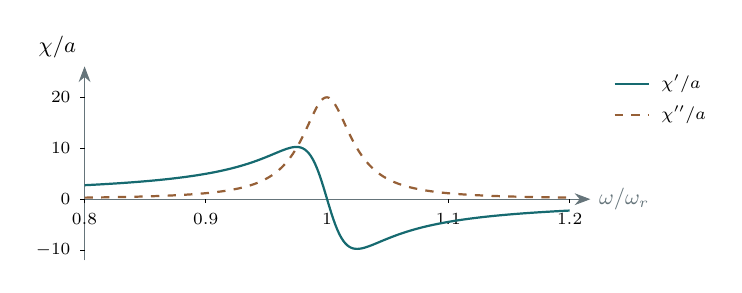
\begin{tikzpicture}[scale=.88,transform shape]
\draw[axis] (0,0.8823529411764706)--(7.3,0.8823529411764706) node[right] {$\omega/\omega_r$};
\draw[axis] (0,0)--(0,2.8);
\node[above left] at (0,2.8) {$\chi/a$};
\draw[thin] (0.000000,0.8823529411764706)--(0.000000,0.8223529411764705);\node[below,font=\scriptsize] at (0.000000,0.8023529411764706) {$ 0.8 $};
\draw[thin] (1.750000,0.8823529411764706)--(1.750000,0.8223529411764705);\node[below,font=\scriptsize] at (1.750000,0.8023529411764706) {$ 0.9 $};
\draw[thin] (3.500000,0.8823529411764706)--(3.500000,0.8223529411764705);\node[below,font=\scriptsize] at (3.500000,0.8023529411764706) {$ 1 $};
\draw[thin] (5.250000,0.8823529411764706)--(5.250000,0.8223529411764705);\node[below,font=\scriptsize] at (5.250000,0.8023529411764706) {$ 1.1 $};
\draw[thin] (7.000000,0.8823529411764706)--(7.000000,0.8223529411764705);\node[below,font=\scriptsize] at (7.000000,0.8023529411764706) {$ 1.2 $};
\draw[thin] (0,0.147059)--(-.06,0.147059);\node[left,font=\scriptsize] at (-.08,0.147059) {$ -10 $};
\draw[thin] (0,0.882353)--(-.06,0.882353);\node[left,font=\scriptsize] at (-.08,0.882353) {$ 0 $};
\draw[thin] (0,1.617647)--(-.06,1.617647);\node[left,font=\scriptsize] at (-.08,1.617647) {$ 10 $};
\draw[thin] (0,2.352941)--(-.06,2.352941);\node[left,font=\scriptsize] at (-.08,2.352941) {$ 20 $};
\draw[thick,color=accent] plot coordinates {(0.0000000,1.0841105) (0.0291667,1.0855700) (0.0583333,1.0870536) (0.0875000,1.0885616) (0.1166667,1.0900947) (0.1458333,1.0916535) (0.1750000,1.0932386) (0.2041667,1.0948507) (0.2333333,1.0964905) (0.2625000,1.0981586) (0.2916667,1.0998558) (0.3208333,1.1015828) (0.3500000,1.1033403) (0.3791667,1.1051292) (0.4083333,1.1069503) (0.4375000,1.1088044) (0.4666667,1.1106923) (0.4958333,1.1126151) (0.5250000,1.1145736) (0.5541667,1.1165687) (0.5833333,1.1186016) (0.6125000,1.1206732) (0.6416667,1.1227846) (0.6708333,1.1249369) (0.7000000,1.1271313) (0.7291667,1.1293689) (0.7583333,1.1316510) (0.7875000,1.1339790) (0.8166667,1.1363540) (0.8458333,1.1387776) (0.8750000,1.1412511) (0.9041667,1.1437760) (0.9333333,1.1463540) (0.9625000,1.1489865) (0.9916667,1.1516753) (1.0208333,1.1544220) (1.0500000,1.1572286) (1.0791667,1.1600969) (1.1083333,1.1630288) (1.1375000,1.1660263) (1.1666667,1.1690916) (1.1958333,1.1722269) (1.2250000,1.1754344) (1.2541667,1.1787166) (1.2833333,1.1820759) (1.3125000,1.1855149) (1.3416667,1.1890363) (1.3708333,1.1926429) (1.4000000,1.1963376) (1.4291667,1.2001234) (1.4583333,1.2040036) (1.4875000,1.2079814) (1.5166667,1.2120603) (1.5458333,1.2162438) (1.5750000,1.2205358) (1.6041667,1.2249401) (1.6333333,1.2294607) (1.6625000,1.2341020) (1.6916667,1.2388683) (1.7208333,1.2437643) (1.7500000,1.2487946) (1.7791667,1.2539643) (1.8083333,1.2592787) (1.8375000,1.2647429) (1.8666667,1.2703627) (1.8958333,1.2761439) (1.9250000,1.2820924) (1.9541667,1.2882145) (1.9833333,1.2945165) (2.0125000,1.3010052) (2.0416667,1.3076872) (2.0708333,1.3145697) (2.1000000,1.3216596) (2.1291667,1.3289643) (2.1583333,1.3364910) (2.1875000,1.3442472) (2.2166667,1.3522401) (2.2458333,1.3604770) (2.2750000,1.3689649) (2.3041667,1.3777106) (2.3333333,1.3867203) (2.3625000,1.3959995) (2.3916667,1.4055531) (2.4208333,1.4153845) (2.4500000,1.4254958) (2.4791667,1.4358872) (2.5083333,1.4465565) (2.5375000,1.4574982) (2.5666667,1.4687033) (2.5958333,1.4801578) (2.6250000,1.4918422) (2.6541667,1.5037295) (2.6833333,1.5157838) (2.7125000,1.5279585) (2.7416667,1.5401937) (2.7708333,1.5524132) (2.8000000,1.5645214) (2.8291667,1.5763990) (2.8583333,1.5878980) (2.8875000,1.5988364) (2.9166667,1.6089917) (2.9458333,1.6180937) (2.9750000,1.6258164) (3.0041667,1.6317697) (3.0333333,1.6354914) (3.0625000,1.6364396) (3.0916667,1.6339874) (3.1208333,1.6274221) (3.1500000,1.6159502) (3.1791667,1.5987126) (3.2083333,1.5748128) (3.2375000,1.5433624) (3.2666667,1.5035458) (3.2958333,1.4547055) (3.3250000,1.3964435) (3.3541667,1.3287301) (3.3833333,1.2520035) (3.4125000,1.1672385) (3.4416667,1.0759627) (3.4708333,0.9802022) (3.5000000,0.8823529) (3.5291667,0.7849903) (3.5583333,0.6906473) (3.5875000,0.6016008) (3.6166667,0.5197011) (3.6458333,0.4462709) (3.6750000,0.3820784) (3.7041667,0.3273760) (3.7333333,0.2819834) (3.7625000,0.2453927) (3.7916667,0.2168759) (3.8208333,0.1955811) (3.8500000,0.1806105) (3.8791667,0.1710771) (3.9083333,0.1661440) (3.9375000,0.1650468) (3.9666667,0.1671049) (3.9958333,0.1717235) (4.0250000,0.1783915) (4.0541667,0.1866745) (4.0833333,0.1962076) (4.1125000,0.2066866) (4.1416667,0.2178601) (4.1708333,0.2295216) (4.2000000,0.2415026) (4.2291667,0.2536664) (4.2583333,0.2659033) (4.2875000,0.2781251) (4.3166667,0.2902623) (4.3458333,0.3022603) (4.3750000,0.3140766) (4.4041667,0.3256791) (4.4333333,0.3370437) (4.4625000,0.3481530) (4.4916667,0.3589951) (4.5208333,0.3695624) (4.5500000,0.3798507) (4.5791667,0.3898588) (4.6083333,0.3995876) (4.6375000,0.4090398) (4.6666667,0.4182193) (4.6958333,0.4271314) (4.7250000,0.4357817) (4.7541667,0.4441769) (4.7833333,0.4523237) (4.8125000,0.4602293) (4.8416667,0.4679008) (4.8708333,0.4753458) (4.9000000,0.4825715) (4.9291667,0.4895853) (4.9583333,0.4963943) (4.9875000,0.5030056) (5.0166667,0.5094261) (5.0458333,0.5156626) (5.0750000,0.5217216) (5.1041667,0.5276094) (5.1333333,0.5333322) (5.1625000,0.5388960) (5.1916667,0.5443063) (5.2208333,0.5495688) (5.2500000,0.5546887) (5.2791667,0.5596712) (5.3083333,0.5645211) (5.3375000,0.5692432) (5.3666667,0.5738420) (5.3958333,0.5783219) (5.4250000,0.5826869) (5.4541667,0.5869412) (5.4833333,0.5910886) (5.5125000,0.5951327) (5.5416667,0.5990770) (5.5708333,0.6029251) (5.6000000,0.6066801) (5.6291667,0.6103451) (5.6583333,0.6139232) (5.6875000,0.6174172) (5.7166667,0.6208299) (5.7458333,0.6241639) (5.7750000,0.6274218) (5.8041667,0.6306060) (5.8333333,0.6337189) (5.8625000,0.6367627) (5.8916667,0.6397396) (5.9208333,0.6426517) (5.9500000,0.6455009) (5.9791667,0.6482892) (6.0083333,0.6510184) (6.0375000,0.6536904) (6.0666667,0.6563067) (6.0958333,0.6588692) (6.1250000,0.6613793) (6.1541667,0.6638386) (6.1833333,0.6662485) (6.2125000,0.6686105) (6.2416667,0.6709260) (6.2708333,0.6731962) (6.3000000,0.6754224) (6.3291667,0.6776059) (6.3583333,0.6797478) (6.3875000,0.6818492) (6.4166667,0.6839113) (6.4458333,0.6859351) (6.4750000,0.6879217) (6.5041667,0.6898720) (6.5333333,0.6917869) (6.5625000,0.6936675) (6.5916667,0.6955146) (6.6208333,0.6973290) (6.6500000,0.6991117) (6.6791667,0.7008633) (6.7083333,0.7025847) (6.7375000,0.7042767) (6.7666667,0.7059399) (6.7958333,0.7075751) (6.8250000,0.7091829) (6.8541667,0.7107641) (6.8833333,0.7123192) (6.9125000,0.7138489) (6.9416667,0.7153537) (6.9708333,0.7168344) (7.0000000,0.7182914)};
\draw[thick,color=accent] (7.65,2.55)--(8.15,2.55);\node[right,font=\scriptsize] at (8.2,2.55) {$\chi^\prime/a$};
\draw[thick,dashed,color=warm] plot coordinates {(0.0000000,0.9047704) (0.0291667,0.9051487) (0.0583333,0.9055364) (0.0875000,0.9059339) (0.1166667,0.9063414) (0.1458333,0.9067595) (0.1750000,0.9071883) (0.2041667,0.9076283) (0.2333333,0.9080798) (0.2625000,0.9085433) (0.2916667,0.9090193) (0.3208333,0.9095080) (0.3500000,0.9100101) (0.3791667,0.9105259) (0.4083333,0.9110561) (0.4375000,0.9116011) (0.4666667,0.9121614) (0.4958333,0.9127377) (0.5250000,0.9133306) (0.5541667,0.9139407) (0.5833333,0.9145687) (0.6125000,0.9152152) (0.6416667,0.9158810) (0.6708333,0.9165670) (0.7000000,0.9172738) (0.7291667,0.9180023) (0.7583333,0.9187535) (0.7875000,0.9195282) (0.8166667,0.9203275) (0.8458333,0.9211524) (0.8750000,0.9220040) (0.9041667,0.9228835) (0.9333333,0.9237920) (0.9625000,0.9247308) (0.9916667,0.9257013) (1.0208333,0.9267050) (1.0500000,0.9277433) (1.0791667,0.9288179) (1.1083333,0.9299303) (1.1375000,0.9310825) (1.1666667,0.9322762) (1.1958333,0.9335135) (1.2250000,0.9347966) (1.2541667,0.9361276) (1.2833333,0.9375089) (1.3125000,0.9389432) (1.3416667,0.9404330) (1.3708333,0.9419813) (1.4000000,0.9435911) (1.4291667,0.9452656) (1.4583333,0.9470084) (1.4875000,0.9488231) (1.5166667,0.9507136) (1.5458333,0.9526842) (1.5750000,0.9547394) (1.6041667,0.9568839) (1.6333333,0.9591230) (1.6625000,0.9614622) (1.6916667,0.9639074) (1.7208333,0.9664650) (1.7500000,0.9691418) (1.7791667,0.9719451) (1.8083333,0.9748829) (1.8375000,0.9779636) (1.8666667,0.9811966) (1.8958333,0.9845916) (1.9250000,0.9881595) (1.9541667,0.9919117) (1.9833333,0.9958609) (2.0125000,1.0000205) (2.0416667,1.0044054) (2.0708333,1.0090315) (2.1000000,1.0139161) (2.1291667,1.0190783) (2.1583333,1.0245384) (2.1875000,1.0303191) (2.2166667,1.0364446) (2.2458333,1.0429417) (2.2750000,1.0498397) (2.3041667,1.0571703) (2.3333333,1.0649687) (2.3625000,1.0732731) (2.3916667,1.0821254) (2.4208333,1.0915719) (2.4500000,1.1016632) (2.4791667,1.1124549) (2.5083333,1.1240081) (2.5375000,1.1363900) (2.5666667,1.1496745) (2.5958333,1.1639427) (2.6250000,1.1792836) (2.6541667,1.1957950) (2.6833333,1.2135838) (2.7125000,1.2327669) (2.7416667,1.2534713) (2.7708333,1.2758351) (2.8000000,1.3000071) (2.8291667,1.3261466) (2.8583333,1.3544223) (2.8875000,1.3850113) (2.9166667,1.4180951) (2.9458333,1.4538562) (2.9750000,1.4924710) (3.0041667,1.5341007) (3.0333333,1.5788788) (3.0625000,1.6268942) (3.0916667,1.6781692) (3.1208333,1.7326327) (3.1500000,1.7900869) (3.1791667,1.8501696) (3.2083333,1.9123143) (3.2375000,1.9757104) (3.2666667,2.0392726) (3.2958333,2.1016263) (3.3250000,2.1611208) (3.3541667,2.2158815) (3.3833333,2.2639066) (3.4125000,2.3032108) (3.4416667,2.3320017) (3.4708333,2.3488675) (3.5000000,2.3529412) (3.5291667,2.3440088) (3.5583333,2.3225372) (3.5875000,2.2896141) (3.6166667,2.2468153) (3.6458333,2.1960275) (3.6750000,2.1392617) (3.7041667,2.0784863) (3.7333333,2.0155008) (3.7625000,1.9518561) (3.7916667,1.8888183) (3.8208333,1.8273666) (3.8500000,1.7682160) (3.8791667,1.7118515) (3.9083333,1.6585691) (3.9375000,1.6085147) (3.9666667,1.5617210) (3.9958333,1.5181377) (4.0250000,1.4776570) (4.0541667,1.4401332) (4.0833333,1.4053982) (4.1125000,1.3732723) (4.1416667,1.3435728) (4.1708333,1.3161194) (4.2000000,1.2907380) (4.2291667,1.2672630) (4.2583333,1.2455392) (4.2875000,1.2254217) (4.3166667,1.2067767) (4.3458333,1.1894809) (4.3750000,1.1734213) (4.4041667,1.1584944) (4.4333333,1.1446060) (4.4625000,1.1316699) (4.4916667,1.1196078) (4.5208333,1.1083485) (4.5500000,1.0978272) (4.5791667,1.0879848) (4.6083333,1.0787675) (4.6375000,1.0701267) (4.6666667,1.0620176) (4.6958333,1.0543997) (4.7250000,1.0472360) (4.7541667,1.0404928) (4.7833333,1.0341391) (4.8125000,1.0281467) (4.8416667,1.0224898) (4.8708333,1.0171447) (4.9000000,1.0120897) (4.9291667,1.0073049) (4.9583333,1.0027720) (4.9875000,0.9984742) (5.0166667,0.9943960) (5.0458333,0.9905230) (5.0750000,0.9868421) (5.1041667,0.9833411) (5.1333333,0.9800089) (5.1625000,0.9768349) (5.1916667,0.9738096) (5.2208333,0.9709239) (5.2500000,0.9681698) (5.2791667,0.9655393) (5.3083333,0.9630254) (5.3375000,0.9606215) (5.3666667,0.9583213) (5.3958333,0.9561191) (5.4250000,0.9540094) (5.4541667,0.9519873) (5.4833333,0.9500480) (5.5125000,0.9481872) (5.5416667,0.9464007) (5.5708333,0.9446847) (5.6000000,0.9430357) (5.6291667,0.9414501) (5.6583333,0.9399249) (5.6875000,0.9384570) (5.7166667,0.9370437) (5.7458333,0.9356823) (5.7750000,0.9343703) (5.8041667,0.9331055) (5.8333333,0.9318855) (5.8625000,0.9307084) (5.8916667,0.9295721) (5.9208333,0.9284749) (5.9500000,0.9274149) (5.9791667,0.9263906) (6.0083333,0.9254003) (6.0375000,0.9244426) (6.0666667,0.9235161) (6.0958333,0.9226194) (6.1250000,0.9217513) (6.1541667,0.9209107) (6.1833333,0.9200963) (6.2125000,0.9193071) (6.2416667,0.9185421) (6.2708333,0.9178004) (6.3000000,0.9170809) (6.3291667,0.9163828) (6.3583333,0.9157053) (6.3875000,0.9150476) (6.4166667,0.9144089) (6.4458333,0.9137885) (6.4750000,0.9131858) (6.5041667,0.9126000) (6.5333333,0.9120305) (6.5625000,0.9114768) (6.5916667,0.9109383) (6.6208333,0.9104143) (6.6500000,0.9099045) (6.6791667,0.9094083) (6.7083333,0.9089252) (6.7375000,0.9084548) (6.7666667,0.9079966) (6.7958333,0.9075502) (6.8250000,0.9071153) (6.8541667,0.9066914) (6.8833333,0.9062781) (6.9125000,0.9058752) (6.9416667,0.9054823) (6.9708333,0.9050989) (7.0000000,0.9047250)};
\draw[thick,dashed,color=warm] (7.65,2.0999999999999996)--(8.15,2.0999999999999996);\node[right,font=\scriptsize] at (8.2,2.0999999999999996) {$\chi^{\prime\prime}/a$};
\end{tikzpicture}
\figcaption{解图光5.2D\quad 含阻尼模型示例：$\gamma=0.05\omega_r$}
\end{minipage}\end{center}


\Needspace{13\baselineskip}

\pdfbookmark[2]{第 3 题 双共振色散与质量比}{q3}

\section*{第 3 题\quad 双共振色散与质量比}\label{q:3}

氟化钙在$0.3$至$10\,\mu\mathrm m$波段有经验关系
\[
n^2=6.09+\frac{6.12\times10^{-15}}{\lambda_0^2-8.88\times10^{-15}}
+\frac{5.10\times10^{-9}}{\lambda_0^2-1.26\times10^{-9}},
\]
式中长度均以m计。求两个有效共振吸收波长。再在两类振子数相等、有效电荷大小相等的近似下，以第一类质量为$m_e$、第二类为Ca与F相对振动的约化质量，估算$m_{\mathrm H}/m_e$。取Ca、F相对原子质量40、19，并检查经验式常数项与双振子模型的关系。

\begin{center}\begin{minipage}{.98\linewidth}\centering
\begin{tikzpicture}[scale=.9,transform shape]
\draw[object] (0.80000,0.00000) circle(0.36000);\draw[object] (4.00000,0.00000) circle(0.25000);\draw[object] plot coordinates {(1.16000,0.00000) (1.34500,0.13000) (1.53000,-0.13000) (1.71500,0.13000) (1.90000,-0.13000) (2.08500,0.13000) (2.27000,-0.13000) (2.45500,0.13000) (2.64000,-0.13000) (2.82500,0.13000) (3.01000,-0.13000) (3.19500,0.13000) (3.38000,-0.13000) (3.56500,0.13000) (3.75000,0.00000)};\node[above] at (0.80000,0.50000) {Ca};\node[above] at (4.00000,0.50000) {F};\draw[force] (0.80000,-0.50000)--(0.20000,-0.50000);\draw[force] (4.00000,-0.50000)--(4.90000,-0.50000);\draw[<->,thin,color=muted] (0.80000,-1.10000)--(4.00000,-1.10000);\node[below] at (2.40000,-1.10000) {相对位移 $x_{\rm Ca}-x_{\rm F}$};\node[above] at (2.40000,1.10000) {$\mu=m_{\rm Ca}m_{\rm F}/(m_{\rm Ca}+m_{\rm F})$};
\end{tikzpicture}
\figcaption{图光5.3\quad Ca与F的相对运动使用约化质量。}
\end{minipage}\end{center}

\Needspace{6\baselineskip}\subsection*{解答}


图光5.3把Ca与F的相对振动写成一个有效离子振子，另用一个快电子振子描述紫外响应。按题设近似，Ca提供的两个价电子与两个F相关的有效离子振子对应等数计数，取$N_1=N_2$、$|q_1|=|q_2|=e$，第一类质量$m_1=m_e$，第二类质量由两体相对运动确定。这些条件用于把光学响应强度转成质量比。

对第$j$类定义
\[
C_j=\frac{N_jq_j^2}{4\pi^2\varepsilon_0m_jc^2},\qquad
\lambda_j=\frac{2\pi c}{\omega_j}.
\]
由受迫振子响应$N_jq_j^2/[\varepsilon_0m_j(\omega_j^2-\omega^2)]$，以真空波长$\lambda_0=2\pi c/\omega$改写，并允许远处共振在所给波段贡献近似常数背景$\varepsilon_b$：
\[
n^2=\varepsilon_b+
\sum_{j=1}^2 C_j\frac{\lambda_0^2\lambda_j^2}{\lambda_0^2-\lambda_j^2}
=\varepsilon_b+\sum_j C_j\lambda_j^2+
\sum_j\frac{C_j\lambda_j^4}{\lambda_0^2-\lambda_j^2}.
\]
第二个等号使用$\lambda_0^2/(\lambda_0^2-\lambda_j^2)=1+\lambda_j^2/(\lambda_0^2-\lambda_j^2)$，因此转换同时产生常数和极点残数。两分母的零点给有效共振波长
\[
\boxed{\lambda_1=\sqrt{8.88\times10^{-15}}=94.23\,\mathrm{nm}},
\qquad
\boxed{\lambda_2=\sqrt{1.26\times10^{-9}}=35.50\,\mu\mathrm m}.
\]
第一处约94.2nm在紫外，第二处约35.5微米在红外，分别位于0.3至10微米测量窗口两侧。解图光5.3A把两极点、窗口和残数的四次方关系放在一起，便于从波长尺度连接两类振动。
\begin{center}\begin{minipage}{.98\linewidth}\centering
\begin{tikzpicture}[scale=.9,transform shape]
\draw[axis] (0.00000,0.00000)--(8.50000,0.00000);\node[below right] at (8.50000,0.00000) {$\log\lambda_0$};\draw[force] (0.71509,-0.10000)--(0.71509,1.10000);\node[above] at (0.71509,1.15000) {$\lambda_1=94.23\,\mathrm{nm}$};\draw[force] (7.40772,-0.10000)--(7.40772,1.10000);\node[above] at (7.40772,1.15000) {$\lambda_2=35.50\,\mu\mathrm m$};\draw[very thick,color=accent] (2.02171,0.38000)--(5.97829,0.38000);\draw[<->,thin,color=muted] (2.02171,-0.45000)--(5.97829,-0.45000);\node[below] at (4.00000,-0.45000) {测量波段};\node[above] at (4.00000,-2.00000) {$A_j=C_j\lambda_j^4$；常数项另含 $\varepsilon_b$};
\end{tikzpicture}
\figcaption{解图光5.3A\quad 分母确定共振位置，残数确定振子强度。}
\end{minipage}\end{center}
无阻尼色散模型在这两个波长有极点，有限阻尼把响应变为有宽度的吸收带。测量窗口内，电子响应为正，离子响应在其本征频率以上为负；解图光5.3B分别画出两振子对$n^2$的实际贡献，二者与$\varepsilon_b$相加给题设折射率平方。
\begin{center}\begin{minipage}{.98\linewidth}\centering
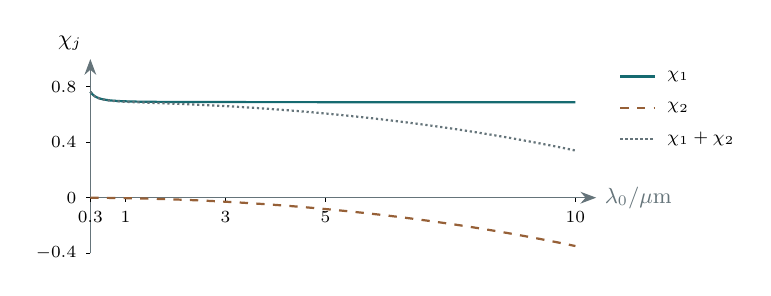
\begin{tikzpicture}[scale=.88,transform shape]
\draw[axis] (0,0.8)--(7.3,0.8) node[right] {$\lambda_0/{\rm \mu m}$};
\draw[axis] (0,0)--(0,2.8);
\node[above left] at (0,2.8) {$\chi_j$};
\draw[thin] (0.000000,0.8)--(0.000000,0.74);\node[below,font=\scriptsize] at (0.000000,0.7200000000000001) {$ 0.3 $};
\draw[thin] (0.505155,0.8)--(0.505155,0.74);\node[below,font=\scriptsize] at (0.505155,0.7200000000000001) {$ 1 $};
\draw[thin] (1.948454,0.8)--(1.948454,0.74);\node[below,font=\scriptsize] at (1.948454,0.7200000000000001) {$ 3 $};
\draw[thin] (3.391753,0.8)--(3.391753,0.74);\node[below,font=\scriptsize] at (3.391753,0.7200000000000001) {$ 5 $};
\draw[thin] (7.000000,0.8)--(7.000000,0.74);\node[below,font=\scriptsize] at (7.000000,0.7200000000000001) {$ 10 $};
\draw[thin] (0,0.000000)--(-.06,0.000000);\node[left,font=\scriptsize] at (-.08,0.000000) {$ -0.4 $};
\draw[thin] (0,0.800000)--(-.06,0.800000);\node[left,font=\scriptsize] at (-.08,0.800000) {$ 0 $};
\draw[thin] (0,1.600000)--(-.06,1.600000);\node[left,font=\scriptsize] at (-.08,1.600000) {$ 0.4 $};
\draw[thin] (0,2.400000)--(-.06,2.400000);\node[left,font=\scriptsize] at (-.08,2.400000) {$ 0.8 $};
\draw[thick,color=accent] plot coordinates {(0.0000000,2.3292660) (0.0291667,2.2927672) (0.0583333,2.2682766) (0.0875000,2.2509885) (0.1166667,2.2383031) (0.1458333,2.2287057) (0.1750000,2.2212616) (0.2041667,2.2153671) (0.2333333,2.2106174) (0.2625000,2.2067324) (0.2916667,2.2035134) (0.3208333,2.2008155) (0.3500000,2.1985317) (0.3791667,2.1965809) (0.4083333,2.1949013) (0.4375000,2.1934447) (0.4666667,2.1921731) (0.4958333,2.1910564) (0.5250000,2.1900703) (0.5541667,2.1891952) (0.5833333,2.1884151) (0.6125000,2.1877166) (0.6416667,2.1870887) (0.6708333,2.1865221) (0.7000000,2.1860092) (0.7291667,2.1855433) (0.7583333,2.1851189) (0.7875000,2.1847312) (0.8166667,2.1843761) (0.8458333,2.1840499) (0.8750000,2.1837497) (0.9041667,2.1834727) (0.9333333,2.1832166) (0.9625000,2.1829794) (0.9916667,2.1827593) (1.0208333,2.1825545) (1.0500000,2.1823639) (1.0791667,2.1821860) (1.1083333,2.1820197) (1.1375000,2.1818641) (1.1666667,2.1817183) (1.1958333,2.1815815) (1.2250000,2.1814529) (1.2541667,2.1813319) (1.2833333,2.1812179) (1.3125000,2.1811104) (1.3416667,2.1810089) (1.3708333,2.1809129) (1.4000000,2.1808221) (1.4291667,2.1807361) (1.4583333,2.1806546) (1.4875000,2.1805772) (1.5166667,2.1805037) (1.5458333,2.1804338) (1.5750000,2.1803674) (1.6041667,2.1803040) (1.6333333,2.1802437) (1.6625000,2.1801862) (1.6916667,2.1801313) (1.7208333,2.1800788) (1.7500000,2.1800287) (1.7791667,2.1799808) (1.8083333,2.1799349) (1.8375000,2.1798909) (1.8666667,2.1798488) (1.8958333,2.1798085) (1.9250000,2.1797697) (1.9541667,2.1797326) (1.9833333,2.1796969) (2.0125000,2.1796625) (2.0416667,2.1796296) (2.0708333,2.1795978) (2.1000000,2.1795673) (2.1291667,2.1795379) (2.1583333,2.1795095) (2.1875000,2.1794822) (2.2166667,2.1794559) (2.2458333,2.1794305) (2.2750000,2.1794060) (2.3041667,2.1793823) (2.3333333,2.1793595) (2.3625000,2.1793374) (2.3916667,2.1793161) (2.4208333,2.1792954) (2.4500000,2.1792755) (2.4791667,2.1792561) (2.5083333,2.1792374) (2.5375000,2.1792193) (2.5666667,2.1792018) (2.5958333,2.1791848) (2.6250000,2.1791683) (2.6541667,2.1791523) (2.6833333,2.1791368) (2.7125000,2.1791218) (2.7416667,2.1791072) (2.7708333,2.1790930) (2.8000000,2.1790793) (2.8291667,2.1790659) (2.8583333,2.1790529) (2.8875000,2.1790403) (2.9166667,2.1790280) (2.9458333,2.1790161) (2.9750000,2.1790045) (3.0041667,2.1789932) (3.0333333,2.1789822) (3.0625000,2.1789715) (3.0916667,2.1789611) (3.1208333,2.1789509) (3.1500000,2.1789411) (3.1791667,2.1789314) (3.2083333,2.1789220) (3.2375000,2.1789129) (3.2666667,2.1789040) (3.2958333,2.1788953) (3.3250000,2.1788868) (3.3541667,2.1788785) (3.3833333,2.1788704) (3.4125000,2.1788626) (3.4416667,2.1788549) (3.4708333,2.1788474) (3.5000000,2.1788400) (3.5291667,2.1788329) (3.5583333,2.1788259) (3.5875000,2.1788190) (3.6166667,2.1788123) (3.6458333,2.1788058) (3.6750000,2.1787994) (3.7041667,2.1787932) (3.7333333,2.1787871) (3.7625000,2.1787811) (3.7916667,2.1787753) (3.8208333,2.1787696) (3.8500000,2.1787640) (3.8791667,2.1787585) (3.9083333,2.1787531) (3.9375000,2.1787479) (3.9666667,2.1787427) (3.9958333,2.1787377) (4.0250000,2.1787328) (4.0541667,2.1787280) (4.0833333,2.1787232) (4.1125000,2.1787186) (4.1416667,2.1787141) (4.1708333,2.1787096) (4.2000000,2.1787053) (4.2291667,2.1787010) (4.2583333,2.1786968) (4.2875000,2.1786927) (4.3166667,2.1786886) (4.3458333,2.1786847) (4.3750000,2.1786808) (4.4041667,2.1786770) (4.4333333,2.1786733) (4.4625000,2.1786696) (4.4916667,2.1786660) (4.5208333,2.1786625) (4.5500000,2.1786590) (4.5791667,2.1786556) (4.6083333,2.1786523) (4.6375000,2.1786490) (4.6666667,2.1786458) (4.6958333,2.1786426) (4.7250000,2.1786395) (4.7541667,2.1786364) (4.7833333,2.1786334) (4.8125000,2.1786305) (4.8416667,2.1786276) (4.8708333,2.1786247) (4.9000000,2.1786219) (4.9291667,2.1786192) (4.9583333,2.1786165) (4.9875000,2.1786138) (5.0166667,2.1786112) (5.0458333,2.1786086) (5.0750000,2.1786061) (5.1041667,2.1786036) (5.1333333,2.1786011) (5.1625000,2.1785987) (5.1916667,2.1785964) (5.2208333,2.1785940) (5.2500000,2.1785917) (5.2791667,2.1785895) (5.3083333,2.1785872) (5.3375000,2.1785851) (5.3666667,2.1785829) (5.3958333,2.1785808) (5.4250000,2.1785787) (5.4541667,2.1785766) (5.4833333,2.1785746) (5.5125000,2.1785726) (5.5416667,2.1785707) (5.5708333,2.1785687) (5.6000000,2.1785668) (5.6291667,2.1785649) (5.6583333,2.1785631) (5.6875000,2.1785613) (5.7166667,2.1785595) (5.7458333,2.1785577) (5.7750000,2.1785560) (5.8041667,2.1785543) (5.8333333,2.1785526) (5.8625000,2.1785509) (5.8916667,2.1785492) (5.9208333,2.1785476) (5.9500000,2.1785460) (5.9791667,2.1785445) (6.0083333,2.1785429) (6.0375000,2.1785414) (6.0666667,2.1785399) (6.0958333,2.1785384) (6.1250000,2.1785369) (6.1541667,2.1785355) (6.1833333,2.1785340) (6.2125000,2.1785326) (6.2416667,2.1785312) (6.2708333,2.1785299) (6.3000000,2.1785285) (6.3291667,2.1785272) (6.3583333,2.1785259) (6.3875000,2.1785246) (6.4166667,2.1785233) (6.4458333,2.1785220) (6.4750000,2.1785208) (6.5041667,2.1785195) (6.5333333,2.1785183) (6.5625000,2.1785171) (6.5916667,2.1785159) (6.6208333,2.1785147) (6.6500000,2.1785136) (6.6791667,2.1785124) (6.7083333,2.1785113) (6.7375000,2.1785102) (6.7666667,2.1785091) (6.7958333,2.1785080) (6.8250000,2.1785069) (6.8541667,2.1785059) (6.8833333,2.1785048) (6.9125000,2.1785038) (6.9416667,2.1785028) (6.9708333,2.1785018) (7.0000000,2.1785008)};
\draw[thick,color=accent] (7.65,2.55)--(8.15,2.55);\node[right,font=\scriptsize] at (8.2,2.55) {$\chi_1$};
\draw[thick,dashed,color=warm] plot coordinates {(0.0000000,0.7994217) (0.0291667,0.7992554) (0.0583333,0.7990681) (0.0875000,0.7988598) (0.1166667,0.7986304) (0.1458333,0.7983801) (0.1750000,0.7981087) (0.2041667,0.7978163) (0.2333333,0.7975029) (0.2625000,0.7971685) (0.2916667,0.7968130) (0.3208333,0.7964365) (0.3500000,0.7960389) (0.3791667,0.7956203) (0.4083333,0.7951807) (0.4375000,0.7947199) (0.4666667,0.7942381) (0.4958333,0.7937353) (0.5250000,0.7932113) (0.5541667,0.7926662) (0.5833333,0.7921001) (0.6125000,0.7915128) (0.6416667,0.7909044) (0.6708333,0.7902748) (0.7000000,0.7896242) (0.7291667,0.7889523) (0.7583333,0.7882594) (0.7875000,0.7875452) (0.8166667,0.7868098) (0.8458333,0.7860533) (0.8750000,0.7852756) (0.9041667,0.7844766) (0.9333333,0.7836564) (0.9625000,0.7828149) (0.9916667,0.7819522) (1.0208333,0.7810683) (1.0500000,0.7801630) (1.0791667,0.7792364) (1.1083333,0.7782886) (1.1375000,0.7773193) (1.1666667,0.7763288) (1.1958333,0.7753169) (1.2250000,0.7742836) (1.2541667,0.7732289) (1.2833333,0.7721528) (1.3125000,0.7710553) (1.3416667,0.7699364) (1.3708333,0.7687960) (1.4000000,0.7676341) (1.4291667,0.7664507) (1.4583333,0.7652458) (1.4875000,0.7640193) (1.5166667,0.7627714) (1.5458333,0.7615018) (1.5750000,0.7602106) (1.6041667,0.7588979) (1.6333333,0.7575635) (1.6625000,0.7562074) (1.6916667,0.7548297) (1.7208333,0.7534302) (1.7500000,0.7520091) (1.7791667,0.7505662) (1.8083333,0.7491015) (1.8375000,0.7476151) (1.8666667,0.7461068) (1.8958333,0.7445767) (1.9250000,0.7430247) (1.9541667,0.7414509) (1.9833333,0.7398551) (2.0125000,0.7382374) (2.0416667,0.7365978) (2.0708333,0.7349361) (2.1000000,0.7332524) (2.1291667,0.7315467) (2.1583333,0.7298190) (2.1875000,0.7280691) (2.2166667,0.7262971) (2.2458333,0.7245030) (2.2750000,0.7226866) (2.3041667,0.7208481) (2.3333333,0.7189873) (2.3625000,0.7171043) (2.3916667,0.7151990) (2.4208333,0.7132713) (2.4500000,0.7113213) (2.4791667,0.7093488) (2.5083333,0.7073540) (2.5375000,0.7053367) (2.5666667,0.7032969) (2.5958333,0.7012346) (2.6250000,0.6991497) (2.6541667,0.6970422) (2.6833333,0.6949122) (2.7125000,0.6927594) (2.7416667,0.6905840) (2.7708333,0.6883858) (2.8000000,0.6861649) (2.8291667,0.6839212) (2.8583333,0.6816546) (2.8875000,0.6793652) (2.9166667,0.6770529) (2.9458333,0.6747176) (2.9750000,0.6723593) (3.0041667,0.6699781) (3.0333333,0.6675737) (3.0625000,0.6651463) (3.0916667,0.6626957) (3.1208333,0.6602219) (3.1500000,0.6577249) (3.1791667,0.6552047) (3.2083333,0.6526611) (3.2375000,0.6500942) (3.2666667,0.6475039) (3.2958333,0.6448902) (3.3250000,0.6422530) (3.3541667,0.6395923) (3.3833333,0.6369080) (3.4125000,0.6342001) (3.4416667,0.6314686) (3.4708333,0.6287134) (3.5000000,0.6259344) (3.5291667,0.6231317) (3.5583333,0.6203051) (3.5875000,0.6174547) (3.6166667,0.6145803) (3.6458333,0.6116819) (3.6750000,0.6087595) (3.7041667,0.6058131) (3.7333333,0.6028425) (3.7625000,0.5998478) (3.7916667,0.5968288) (3.8208333,0.5937856) (3.8500000,0.5907180) (3.8791667,0.5876261) (3.9083333,0.5845097) (3.9375000,0.5813689) (3.9666667,0.5782035) (3.9958333,0.5750136) (4.0250000,0.5717990) (4.0541667,0.5685597) (4.0833333,0.5652957) (4.1125000,0.5620069) (4.1416667,0.5586932) (4.1708333,0.5553546) (4.2000000,0.5519910) (4.2291667,0.5486024) (4.2583333,0.5451887) (4.2875000,0.5417499) (4.3166667,0.5382859) (4.3458333,0.5347966) (4.3750000,0.5312820) (4.4041667,0.5277420) (4.4333333,0.5241765) (4.4625000,0.5205856) (4.4916667,0.5169691) (4.5208333,0.5133270) (4.5500000,0.5096591) (4.5791667,0.5059656) (4.6083333,0.5022462) (4.6375000,0.4985009) (4.6666667,0.4947297) (4.6958333,0.4909324) (4.7250000,0.4871091) (4.7541667,0.4832597) (4.7833333,0.4793840) (4.8125000,0.4754820) (4.8416667,0.4715537) (4.8708333,0.4675990) (4.9000000,0.4636178) (4.9291667,0.4596101) (4.9583333,0.4555757) (4.9875000,0.4515146) (5.0166667,0.4474268) (5.0458333,0.4433121) (5.0750000,0.4391705) (5.1041667,0.4350019) (5.1333333,0.4308063) (5.1625000,0.4265835) (5.1916667,0.4223335) (5.2208333,0.4180562) (5.2500000,0.4137516) (5.2791667,0.4094195) (5.3083333,0.4050599) (5.3375000,0.4006727) (5.3666667,0.3962579) (5.3958333,0.3918153) (5.4250000,0.3873449) (5.4541667,0.3828465) (5.4833333,0.3783202) (5.5125000,0.3737657) (5.5416667,0.3691832) (5.5708333,0.3645724) (5.6000000,0.3599332) (5.6291667,0.3552657) (5.6583333,0.3505696) (5.6875000,0.3458450) (5.7166667,0.3410918) (5.7458333,0.3363097) (5.7750000,0.3314989) (5.8041667,0.3266591) (5.8333333,0.3217902) (5.8625000,0.3168923) (5.8916667,0.3119652) (5.9208333,0.3070088) (5.9500000,0.3020230) (5.9791667,0.2970078) (6.0083333,0.2919629) (6.0375000,0.2868885) (6.0666667,0.2817842) (6.0958333,0.2766502) (6.1250000,0.2714861) (6.1541667,0.2662921) (6.1833333,0.2610679) (6.2125000,0.2558134) (6.2416667,0.2505287) (6.2708333,0.2452134) (6.3000000,0.2398677) (6.3291667,0.2344913) (6.3583333,0.2290842) (6.3875000,0.2236463) (6.4166667,0.2181773) (6.4458333,0.2126774) (6.4750000,0.2071463) (6.5041667,0.2015839) (6.5333333,0.1959902) (6.5625000,0.1903650) (6.5916667,0.1847082) (6.6208333,0.1790197) (6.6500000,0.1732995) (6.6791667,0.1675473) (6.7083333,0.1617631) (6.7375000,0.1559467) (6.7666667,0.1500981) (6.7958333,0.1442172) (6.8250000,0.1383038) (6.8541667,0.1323577) (6.8833333,0.1263790) (6.9125000,0.1203675) (6.9416667,0.1143230) (6.9708333,0.1082454) (7.0000000,0.1021346)};
\draw[thick,dashed,color=warm] (7.65,2.0999999999999996)--(8.15,2.0999999999999996);\node[right,font=\scriptsize] at (8.2,2.0999999999999996) {$\chi_2$};
\draw[densely dotted,thick,color=muted] plot coordinates {(0.0000000,2.3286877) (0.0291667,2.2920226) (0.0583333,2.2673446) (0.0875000,2.2498482) (0.1166667,2.2369336) (0.1458333,2.2270858) (0.1750000,2.2193703) (0.2041667,2.2131834) (0.2333333,2.2081203) (0.2625000,2.2039009) (0.2916667,2.2003264) (0.3208333,2.1972520) (0.3500000,2.1945706) (0.3791667,2.1922013) (0.4083333,2.1900820) (0.4375000,2.1881646) (0.4666667,2.1864112) (0.4958333,2.1847916) (0.5250000,2.1832816) (0.5541667,2.1818615) (0.5833333,2.1805152) (0.6125000,2.1792294) (0.6416667,2.1779930) (0.6708333,2.1767970) (0.7000000,2.1756334) (0.7291667,2.1744957) (0.7583333,2.1733783) (0.7875000,2.1722764) (0.8166667,2.1711859) (0.8458333,2.1701032) (0.8750000,2.1690252) (0.9041667,2.1679493) (0.9333333,2.1668730) (0.9625000,2.1657944) (0.9916667,2.1647115) (1.0208333,2.1636228) (1.0500000,2.1625269) (1.0791667,2.1614224) (1.1083333,2.1603083) (1.1375000,2.1591835) (1.1666667,2.1580471) (1.1958333,2.1568984) (1.2250000,2.1557365) (1.2541667,2.1545608) (1.2833333,2.1533707) (1.3125000,2.1521657) (1.3416667,2.1509453) (1.3708333,2.1497089) (1.4000000,2.1484562) (1.4291667,2.1471868) (1.4583333,2.1459004) (1.4875000,2.1445965) (1.5166667,2.1432751) (1.5458333,2.1419356) (1.5750000,2.1405780) (1.6041667,2.1392019) (1.6333333,2.1378072) (1.6625000,2.1363936) (1.6916667,2.1349609) (1.7208333,2.1335091) (1.7500000,2.1320378) (1.7791667,2.1305469) (1.8083333,2.1290364) (1.8375000,2.1275060) (1.8666667,2.1259556) (1.8958333,2.1243851) (1.9250000,2.1227945) (1.9541667,2.1211834) (1.9833333,2.1195520) (2.0125000,2.1179000) (2.0416667,2.1162273) (2.0708333,2.1145339) (2.1000000,2.1128197) (2.1291667,2.1110846) (2.1583333,2.1093285) (2.1875000,2.1075513) (2.2166667,2.1057530) (2.2458333,2.1039335) (2.2750000,2.1020927) (2.3041667,2.1002305) (2.3333333,2.0983468) (2.3625000,2.0964417) (2.3916667,2.0945150) (2.4208333,2.0925667) (2.4500000,2.0905967) (2.4791667,2.0886050) (2.5083333,2.0865914) (2.5375000,2.0845560) (2.5666667,2.0824987) (2.5958333,2.0804194) (2.6250000,2.0783180) (2.6541667,2.0761946) (2.6833333,2.0740490) (2.7125000,2.0718812) (2.7416667,2.0696912) (2.7708333,2.0674789) (2.8000000,2.0652442) (2.8291667,2.0629871) (2.8583333,2.0607076) (2.8875000,2.0584055) (2.9166667,2.0560809) (2.9458333,2.0537337) (2.9750000,2.0513638) (3.0041667,2.0489712) (3.0333333,2.0465559) (3.0625000,2.0441178) (3.0916667,2.0416567) (3.1208333,2.0391728) (3.1500000,2.0366660) (3.1791667,2.0341361) (3.2083333,2.0315831) (3.2375000,2.0290071) (3.2666667,2.0264079) (3.2958333,2.0237855) (3.3250000,2.0211398) (3.3541667,2.0184708) (3.3833333,2.0157785) (3.4125000,2.0130627) (3.4416667,2.0103235) (3.4708333,2.0075608) (3.5000000,2.0047745) (3.5291667,2.0019646) (3.5583333,1.9991310) (3.5875000,1.9962737) (3.6166667,1.9933926) (3.6458333,1.9904877) (3.6750000,1.9875590) (3.7041667,1.9846063) (3.7333333,1.9816296) (3.7625000,1.9786289) (3.7916667,1.9756041) (3.8208333,1.9725551) (3.8500000,1.9694820) (3.8791667,1.9663846) (3.9083333,1.9632629) (3.9375000,1.9601168) (3.9666667,1.9569463) (3.9958333,1.9537513) (4.0250000,1.9505318) (4.0541667,1.9472877) (4.0833333,1.9440189) (4.1125000,1.9407255) (4.1416667,1.9374073) (4.1708333,1.9340642) (4.2000000,1.9306963) (4.2291667,1.9273034) (4.2583333,1.9238855) (4.2875000,1.9204426) (4.3166667,1.9169745) (4.3458333,1.9134813) (4.3750000,1.9099628) (4.4041667,1.9064190) (4.4333333,1.9028498) (4.4625000,1.8992552) (4.4916667,1.8956351) (4.5208333,1.8919894) (4.5500000,1.8883181) (4.5791667,1.8846212) (4.6083333,1.8808984) (4.6375000,1.8771499) (4.6666667,1.8733754) (4.6958333,1.8695750) (4.7250000,1.8657486) (4.7541667,1.8618961) (4.7833333,1.8580174) (4.8125000,1.8541125) (4.8416667,1.8501813) (4.8708333,1.8462237) (4.9000000,1.8422397) (4.9291667,1.8382292) (4.9583333,1.8341922) (4.9875000,1.8301284) (5.0166667,1.8260380) (5.0458333,1.8219207) (5.0750000,1.8177766) (5.1041667,1.8136055) (5.1333333,1.8094074) (5.1625000,1.8051822) (5.1916667,1.8009298) (5.2208333,1.7966502) (5.2500000,1.7923433) (5.2791667,1.7880090) (5.3083333,1.7836472) (5.3375000,1.7792578) (5.3666667,1.7748408) (5.3958333,1.7703961) (5.4250000,1.7659235) (5.4541667,1.7614231) (5.4833333,1.7568948) (5.5125000,1.7523384) (5.5416667,1.7477538) (5.5708333,1.7431411) (5.6000000,1.7385000) (5.6291667,1.7338306) (5.6583333,1.7291327) (5.6875000,1.7244063) (5.7166667,1.7196512) (5.7458333,1.7148674) (5.7750000,1.7100548) (5.8041667,1.7052133) (5.8333333,1.7003428) (5.8625000,1.6954432) (5.8916667,1.6905145) (5.9208333,1.6855564) (5.9500000,1.6805690) (5.9791667,1.6755522) (6.0083333,1.6705058) (6.0375000,1.6654298) (6.0666667,1.6603241) (6.0958333,1.6551885) (6.1250000,1.6500230) (6.1541667,1.6448275) (6.1833333,1.6396019) (6.2125000,1.6343460) (6.2416667,1.6290599) (6.2708333,1.6237433) (6.3000000,1.6183962) (6.3291667,1.6130185) (6.3583333,1.6076101) (6.3875000,1.6021708) (6.4166667,1.5967006) (6.4458333,1.5911994) (6.4750000,1.5856670) (6.5041667,1.5801034) (6.5333333,1.5745085) (6.5625000,1.5688821) (6.5916667,1.5632241) (6.6208333,1.5575345) (6.6500000,1.5518131) (6.6791667,1.5460597) (6.7083333,1.5402744) (6.7375000,1.5344569) (6.7666667,1.5286072) (6.7958333,1.5227252) (6.8250000,1.5168107) (6.8541667,1.5108636) (6.8833333,1.5048839) (6.9125000,1.4988713) (6.9416667,1.4928257) (6.9708333,1.4867472) (7.0000000,1.4806354)};
\draw[densely dotted,thick,color=muted] (7.65,1.65)--(8.15,1.65);\node[right,font=\scriptsize] at (8.2,1.65) {$\chi_1+\chi_2$};
\end{tikzpicture}
\figcaption{解图光5.3B\quad 电子正响应与离子负响应在透明窗口内共同作用}
\end{minipage}\end{center}
记$a_j=\lambda_j^2$，题给残数为$A_1=6.12\times10^{-15}\,\mathrm{m^2}$、$A_2=5.10\times10^{-9}\,\mathrm{m^2}$。从分式匹配得到$A_j=C_ja_j^2$，所以
\[
\frac{C_2}{C_1}
=\frac{A_2}{A_1}\left(\frac{a_1}{a_2}\right)^2
=\frac{5.10\times10^{-9}}{6.12\times10^{-15}}
\left(\frac{8.88\times10^{-15}}{1.26\times10^{-9}}\right)^2
=4.13908\times10^{-5}.
\]
强度比还包含振子数与有效电荷，一般关系为$C_2/C_1=(N_2/N_1)(q_2^2/q_1^2)(m_e/\mu)$。在已指定的等数、等电荷近似下，才简化为$C_2/C_1=m_e/\mu$。

下面由图中两个相反的回复力推导$\mu$。以$x_{\rm Ca},x_{\rm F}$表示两个离子相对各自平衡位置的位移，设$\zeta=x_{\rm Ca}-x_{\rm F}$，回复力分别为$-\kappa\zeta$、$+\kappa\zeta$，两运动方程相减，得
\[
\ddot\zeta=-\kappa\left(\frac1{m_{\mathrm{Ca}}}
+\frac1{m_{\mathrm F}}\right)\zeta,\qquad
\frac1\mu=\frac1{m_{\mathrm{Ca}}}+\frac1{m_{\mathrm F}}.
\]
因此相对坐标满足$\mu\ddot\zeta+\kappa\zeta=0$，质量为
\[
\mu=\frac{m_{\mathrm{Ca}}m_{\mathrm F}}{m_{\mathrm{Ca}}+m_{\mathrm F}}
=\frac{40\times19}{59}m_{\mathrm H}
=12.88136\,m_{\mathrm H}.
\]
这个系数来自两体相对加速度，质心运动从内部振动中分离。把$\mu=(760/59)m_{\rm H}$与光学强度比结合，有
\[
\boxed{\frac{m_{\mathrm H}}{m_e}
=\frac{59}{760}\frac{C_1}{C_2}
\simeq1.876\times10^3}.
\]
使用题给系数而在中途保留小数，结果为$m_{\rm H}/m_e=1875.58$。解图光5.3C把等数、等电荷条件下的$C_2/C_1$画成质量比的函数，观测水平线在此值相交。该交点在等数、等电荷与上述约化质量条件下确定质量比。
\begin{center}\begin{minipage}{.98\linewidth}\centering
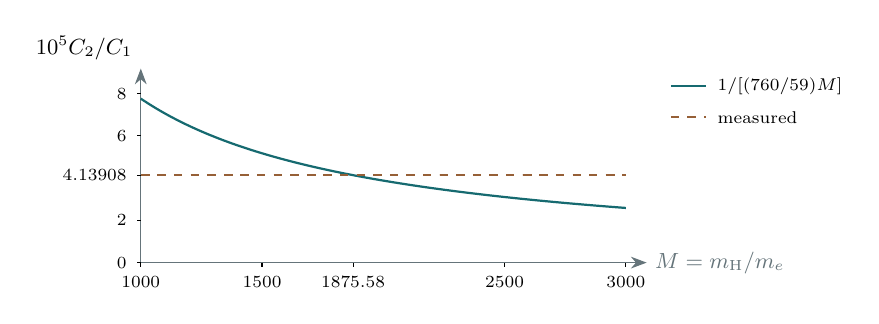
\begin{tikzpicture}[scale=.88,transform shape]
\draw[axis] (0,0.0)--(7.3,0.0) node[right] {$M=m_{\rm H}/m_e$};
\draw[axis] (0,0)--(0,2.8);
\node[above left] at (0,2.8) {$10^5 C_2/C_1$};
\draw[thin] (0.000000,0.0)--(0.000000,-0.06);\node[below,font=\scriptsize] at (0.000000,-0.08) {$ 1000 $};
\draw[thin] (1.750000,0.0)--(1.750000,-0.06);\node[below,font=\scriptsize] at (1.750000,-0.08) {$ 1500 $};
\draw[thin] (3.064530,0.0)--(3.064530,-0.06);\node[below,font=\scriptsize] at (3.064530,-0.08) {$ 1875.58 $};
\draw[thin] (5.250000,0.0)--(5.250000,-0.06);\node[below,font=\scriptsize] at (5.250000,-0.08) {$ 2500 $};
\draw[thin] (7.000000,0.0)--(7.000000,-0.06);\node[below,font=\scriptsize] at (7.000000,-0.08) {$ 3000 $};
\draw[thin] (0,0.000000)--(-.06,0.000000);\node[left,font=\scriptsize] at (-.08,0.000000) {$ 0 $};
\draw[thin] (0,0.609756)--(-.06,0.609756);\node[left,font=\scriptsize] at (-.08,0.609756) {$ 2 $};
\draw[thin] (0,1.261915)--(-.06,1.261915);\node[left,font=\scriptsize] at (-.08,1.261915) {$ 4.13908 $};
\draw[thin] (0,1.829268)--(-.06,1.829268);\node[left,font=\scriptsize] at (-.08,1.829268) {$ 6 $};
\draw[thin] (0,2.439024)--(-.06,2.439024);\node[left,font=\scriptsize] at (-.08,2.439024) {$ 8 $};
\draw[thick,color=accent] plot coordinates {(0.0000000,2.3668164) (0.0291667,2.3472560) (0.0583333,2.3280162) (0.0875000,2.3090892) (0.1166667,2.2904675) (0.1458333,2.2721438) (0.1750000,2.2541109) (0.2041667,2.2363620) (0.2333333,2.2188904) (0.2625000,2.2016897) (0.2916667,2.1847536) (0.3208333,2.1680761) (0.3500000,2.1516513) (0.3791667,2.1354735) (0.4083333,2.1195371) (0.4375000,2.1038368) (0.4666667,2.0883674) (0.4958333,2.0731239) (0.5250000,2.0581012) (0.5541667,2.0432948) (0.5833333,2.0286998) (0.6125000,2.0143119) (0.6416667,2.0001266) (0.6708333,1.9861397) (0.7000000,1.9723470) (0.7291667,1.9587446) (0.7583333,1.9453286) (0.7875000,1.9320950) (0.8166667,1.9190403) (0.8458333,1.9061609) (0.8750000,1.8934531) (0.9041667,1.8809137) (0.9333333,1.8685393) (0.9625000,1.8563266) (0.9916667,1.8442725) (1.0208333,1.8323740) (1.0500000,1.8206280) (1.0791667,1.8090317) (1.1083333,1.7975821) (1.1375000,1.7862766) (1.1666667,1.7751123) (1.1958333,1.7640868) (1.2250000,1.7531974) (1.2541667,1.7424415) (1.2833333,1.7318169) (1.3125000,1.7213210) (1.3416667,1.7109516) (1.3708333,1.7007064) (1.4000000,1.6905832) (1.4291667,1.6805797) (1.4583333,1.6706940) (1.4875000,1.6609238) (1.5166667,1.6512673) (1.5458333,1.6417224) (1.5750000,1.6322872) (1.6041667,1.6229598) (1.6333333,1.6137385) (1.6625000,1.6046213) (1.6916667,1.5956066) (1.7208333,1.5866926) (1.7500000,1.5778776) (1.7791667,1.5691601) (1.8083333,1.5605383) (1.8375000,1.5520108) (1.8666667,1.5435759) (1.8958333,1.5352323) (1.9250000,1.5269783) (1.9541667,1.5188127) (1.9833333,1.5107339) (2.0125000,1.5027406) (2.0416667,1.4948314) (2.0708333,1.4870051) (2.1000000,1.4792603) (2.1291667,1.4715957) (2.1583333,1.4640102) (2.1875000,1.4565024) (2.2166667,1.4490713) (2.2458333,1.4417156) (2.2750000,1.4344342) (2.3041667,1.4272260) (2.3333333,1.4200899) (2.3625000,1.4130247) (2.3916667,1.4060296) (2.4208333,1.3991033) (2.4500000,1.3922450) (2.4791667,1.3854535) (2.5083333,1.3787280) (2.5375000,1.3720675) (2.5666667,1.3654710) (2.5958333,1.3589377) (2.6250000,1.3524665) (2.6541667,1.3460567) (2.6833333,1.3397074) (2.7125000,1.3334177) (2.7416667,1.3271868) (2.7708333,1.3210138) (2.8000000,1.3148980) (2.8291667,1.3088386) (2.8583333,1.3028347) (2.8875000,1.2968857) (2.9166667,1.2909908) (2.9458333,1.2851492) (2.9750000,1.2793602) (3.0041667,1.2736232) (3.0333333,1.2679374) (3.0625000,1.2623021) (3.0916667,1.2567167) (3.1208333,1.2511805) (3.1500000,1.2456929) (3.1791667,1.2402532) (3.2083333,1.2348607) (3.2375000,1.2295150) (3.2666667,1.2242154) (3.2958333,1.2189613) (3.3250000,1.2137520) (3.3541667,1.2085871) (3.3833333,1.2034660) (3.4125000,1.1983881) (3.4416667,1.1933528) (3.4708333,1.1883597) (3.5000000,1.1834082) (3.5291667,1.1784978) (3.5583333,1.1736280) (3.5875000,1.1687982) (3.6166667,1.1640081) (3.6458333,1.1592570) (3.6750000,1.1545446) (3.7041667,1.1498703) (3.7333333,1.1452338) (3.7625000,1.1406344) (3.7916667,1.1360719) (3.8208333,1.1315457) (3.8500000,1.1270554) (3.8791667,1.1226007) (3.9083333,1.1181810) (3.9375000,1.1137960) (3.9666667,1.1094452) (3.9958333,1.1051283) (4.0250000,1.1008449) (4.0541667,1.0965945) (4.0833333,1.0923768) (4.1125000,1.0881915) (4.1416667,1.0840381) (4.1708333,1.0799162) (4.2000000,1.0758257) (4.2291667,1.0717659) (4.2583333,1.0677367) (4.2875000,1.0637377) (4.3166667,1.0597686) (4.3458333,1.0558289) (4.3750000,1.0519184) (4.4041667,1.0480368) (4.4333333,1.0441837) (4.4625000,1.0403589) (4.4916667,1.0365619) (4.5208333,1.0327926) (4.5500000,1.0290506) (4.5791667,1.0253356) (4.6083333,1.0216474) (4.6375000,1.0179856) (4.6666667,1.0143499) (4.6958333,1.0107401) (4.7250000,1.0071559) (4.7541667,1.0035971) (4.7833333,1.0000633) (4.8125000,0.9965543) (4.8416667,0.9930698) (4.8708333,0.9896097) (4.9000000,0.9861735) (4.9291667,0.9827611) (4.9583333,0.9793723) (4.9875000,0.9760068) (5.0166667,0.9726643) (5.0458333,0.9693446) (5.0750000,0.9660475) (5.1041667,0.9627728) (5.1333333,0.9595202) (5.1625000,0.9562895) (5.1916667,0.9530804) (5.2208333,0.9498929) (5.2500000,0.9467266) (5.2791667,0.9435813) (5.3083333,0.9404569) (5.3375000,0.9373530) (5.3666667,0.9342696) (5.3958333,0.9312065) (5.4250000,0.9281633) (5.4541667,0.9251400) (5.4833333,0.9221363) (5.5125000,0.9191520) (5.5416667,0.9161870) (5.5708333,0.9132411) (5.6000000,0.9103140) (5.6291667,0.9074057) (5.6583333,0.9045158) (5.6875000,0.9016444) (5.7166667,0.8987910) (5.7458333,0.8959557) (5.7750000,0.8931383) (5.8041667,0.8903385) (5.8333333,0.8875562) (5.8625000,0.8847912) (5.8916667,0.8820434) (5.9208333,0.8793126) (5.9500000,0.8765987) (5.9791667,0.8739015) (6.0083333,0.8712208) (6.0375000,0.8685565) (6.0666667,0.8659085) (6.0958333,0.8632765) (6.1250000,0.8606605) (6.1541667,0.8580603) (6.1833333,0.8554758) (6.2125000,0.8529068) (6.2416667,0.8503532) (6.2708333,0.8478148) (6.3000000,0.8452916) (6.3291667,0.8427833) (6.3583333,0.8402899) (6.3875000,0.8378111) (6.4166667,0.8353470) (6.4458333,0.8328973) (6.4750000,0.8304619) (6.5041667,0.8280407) (6.5333333,0.8256336) (6.5625000,0.8232405) (6.5916667,0.8208612) (6.6208333,0.8184956) (6.6500000,0.8161436) (6.6791667,0.8138051) (6.7083333,0.8114799) (6.7375000,0.8091680) (6.7666667,0.8068692) (6.7958333,0.8045835) (6.8250000,0.8023107) (6.8541667,0.8000506) (6.8833333,0.7978033) (6.9125000,0.7955685) (6.9416667,0.7933463) (6.9708333,0.7911364) (7.0000000,0.7889388)};
\draw[thick,color=accent] (7.65,2.55)--(8.15,2.55);\node[right,font=\scriptsize] at (8.2,2.55) {$1/[(760/59)M]$};
\draw[thick,dashed,color=warm] plot coordinates {(0.0000000,1.2619140) (0.0291667,1.2619140) (0.0583333,1.2619140) (0.0875000,1.2619140) (0.1166667,1.2619140) (0.1458333,1.2619140) (0.1750000,1.2619140) (0.2041667,1.2619140) (0.2333333,1.2619140) (0.2625000,1.2619140) (0.2916667,1.2619140) (0.3208333,1.2619140) (0.3500000,1.2619140) (0.3791667,1.2619140) (0.4083333,1.2619140) (0.4375000,1.2619140) (0.4666667,1.2619140) (0.4958333,1.2619140) (0.5250000,1.2619140) (0.5541667,1.2619140) (0.5833333,1.2619140) (0.6125000,1.2619140) (0.6416667,1.2619140) (0.6708333,1.2619140) (0.7000000,1.2619140) (0.7291667,1.2619140) (0.7583333,1.2619140) (0.7875000,1.2619140) (0.8166667,1.2619140) (0.8458333,1.2619140) (0.8750000,1.2619140) (0.9041667,1.2619140) (0.9333333,1.2619140) (0.9625000,1.2619140) (0.9916667,1.2619140) (1.0208333,1.2619140) (1.0500000,1.2619140) (1.0791667,1.2619140) (1.1083333,1.2619140) (1.1375000,1.2619140) (1.1666667,1.2619140) (1.1958333,1.2619140) (1.2250000,1.2619140) (1.2541667,1.2619140) (1.2833333,1.2619140) (1.3125000,1.2619140) (1.3416667,1.2619140) (1.3708333,1.2619140) (1.4000000,1.2619140) (1.4291667,1.2619140) (1.4583333,1.2619140) (1.4875000,1.2619140) (1.5166667,1.2619140) (1.5458333,1.2619140) (1.5750000,1.2619140) (1.6041667,1.2619140) (1.6333333,1.2619140) (1.6625000,1.2619140) (1.6916667,1.2619140) (1.7208333,1.2619140) (1.7500000,1.2619140) (1.7791667,1.2619140) (1.8083333,1.2619140) (1.8375000,1.2619140) (1.8666667,1.2619140) (1.8958333,1.2619140) (1.9250000,1.2619140) (1.9541667,1.2619140) (1.9833333,1.2619140) (2.0125000,1.2619140) (2.0416667,1.2619140) (2.0708333,1.2619140) (2.1000000,1.2619140) (2.1291667,1.2619140) (2.1583333,1.2619140) (2.1875000,1.2619140) (2.2166667,1.2619140) (2.2458333,1.2619140) (2.2750000,1.2619140) (2.3041667,1.2619140) (2.3333333,1.2619140) (2.3625000,1.2619140) (2.3916667,1.2619140) (2.4208333,1.2619140) (2.4500000,1.2619140) (2.4791667,1.2619140) (2.5083333,1.2619140) (2.5375000,1.2619140) (2.5666667,1.2619140) (2.5958333,1.2619140) (2.6250000,1.2619140) (2.6541667,1.2619140) (2.6833333,1.2619140) (2.7125000,1.2619140) (2.7416667,1.2619140) (2.7708333,1.2619140) (2.8000000,1.2619140) (2.8291667,1.2619140) (2.8583333,1.2619140) (2.8875000,1.2619140) (2.9166667,1.2619140) (2.9458333,1.2619140) (2.9750000,1.2619140) (3.0041667,1.2619140) (3.0333333,1.2619140) (3.0625000,1.2619140) (3.0916667,1.2619140) (3.1208333,1.2619140) (3.1500000,1.2619140) (3.1791667,1.2619140) (3.2083333,1.2619140) (3.2375000,1.2619140) (3.2666667,1.2619140) (3.2958333,1.2619140) (3.3250000,1.2619140) (3.3541667,1.2619140) (3.3833333,1.2619140) (3.4125000,1.2619140) (3.4416667,1.2619140) (3.4708333,1.2619140) (3.5000000,1.2619140) (3.5291667,1.2619140) (3.5583333,1.2619140) (3.5875000,1.2619140) (3.6166667,1.2619140) (3.6458333,1.2619140) (3.6750000,1.2619140) (3.7041667,1.2619140) (3.7333333,1.2619140) (3.7625000,1.2619140) (3.7916667,1.2619140) (3.8208333,1.2619140) (3.8500000,1.2619140) (3.8791667,1.2619140) (3.9083333,1.2619140) (3.9375000,1.2619140) (3.9666667,1.2619140) (3.9958333,1.2619140) (4.0250000,1.2619140) (4.0541667,1.2619140) (4.0833333,1.2619140) (4.1125000,1.2619140) (4.1416667,1.2619140) (4.1708333,1.2619140) (4.2000000,1.2619140) (4.2291667,1.2619140) (4.2583333,1.2619140) (4.2875000,1.2619140) (4.3166667,1.2619140) (4.3458333,1.2619140) (4.3750000,1.2619140) (4.4041667,1.2619140) (4.4333333,1.2619140) (4.4625000,1.2619140) (4.4916667,1.2619140) (4.5208333,1.2619140) (4.5500000,1.2619140) (4.5791667,1.2619140) (4.6083333,1.2619140) (4.6375000,1.2619140) (4.6666667,1.2619140) (4.6958333,1.2619140) (4.7250000,1.2619140) (4.7541667,1.2619140) (4.7833333,1.2619140) (4.8125000,1.2619140) (4.8416667,1.2619140) (4.8708333,1.2619140) (4.9000000,1.2619140) (4.9291667,1.2619140) (4.9583333,1.2619140) (4.9875000,1.2619140) (5.0166667,1.2619140) (5.0458333,1.2619140) (5.0750000,1.2619140) (5.1041667,1.2619140) (5.1333333,1.2619140) (5.1625000,1.2619140) (5.1916667,1.2619140) (5.2208333,1.2619140) (5.2500000,1.2619140) (5.2791667,1.2619140) (5.3083333,1.2619140) (5.3375000,1.2619140) (5.3666667,1.2619140) (5.3958333,1.2619140) (5.4250000,1.2619140) (5.4541667,1.2619140) (5.4833333,1.2619140) (5.5125000,1.2619140) (5.5416667,1.2619140) (5.5708333,1.2619140) (5.6000000,1.2619140) (5.6291667,1.2619140) (5.6583333,1.2619140) (5.6875000,1.2619140) (5.7166667,1.2619140) (5.7458333,1.2619140) (5.7750000,1.2619140) (5.8041667,1.2619140) (5.8333333,1.2619140) (5.8625000,1.2619140) (5.8916667,1.2619140) (5.9208333,1.2619140) (5.9500000,1.2619140) (5.9791667,1.2619140) (6.0083333,1.2619140) (6.0375000,1.2619140) (6.0666667,1.2619140) (6.0958333,1.2619140) (6.1250000,1.2619140) (6.1541667,1.2619140) (6.1833333,1.2619140) (6.2125000,1.2619140) (6.2416667,1.2619140) (6.2708333,1.2619140) (6.3000000,1.2619140) (6.3291667,1.2619140) (6.3583333,1.2619140) (6.3875000,1.2619140) (6.4166667,1.2619140) (6.4458333,1.2619140) (6.4750000,1.2619140) (6.5041667,1.2619140) (6.5333333,1.2619140) (6.5625000,1.2619140) (6.5916667,1.2619140) (6.6208333,1.2619140) (6.6500000,1.2619140) (6.6791667,1.2619140) (6.7083333,1.2619140) (6.7375000,1.2619140) (6.7666667,1.2619140) (6.7958333,1.2619140) (6.8250000,1.2619140) (6.8541667,1.2619140) (6.8833333,1.2619140) (6.9125000,1.2619140) (6.9416667,1.2619140) (6.9708333,1.2619140) (7.0000000,1.2619140)};
\draw[thick,dashed,color=warm] (7.65,2.0999999999999996)--(8.15,2.0999999999999996);\node[right,font=\scriptsize] at (8.2,2.0999999999999996) {$\mathrm{measured}$};
\end{tikzpicture}
\figcaption{解图光5.3C\quad 等数等电荷模型的质量比由残数比水平线交点确定}
\end{minipage}\end{center}
常数项也由同一次代数分解给出：
\[
C_1a_1+C_2a_2=\frac{A_1}{a_1}+\frac{A_2}{a_2}
=0.689189+4.047619=4.736808.
\]
两个振子配合真空常数1给$1+4.736808=5.736808$。题给总常数6.09相应需要
\[
\boxed{\varepsilon_b=6.09-4.736808=1.353192}.
\]
解图光5.3D在整个测量窗口比较这两个常数选择，$n^2$之间相差$.353192$。额外背景在这一有限波段内近似不随频率变，可由更远处的共振贡献；本次残数和由它们得到的强度比保持不变。
\begin{center}\begin{minipage}{.98\linewidth}\centering
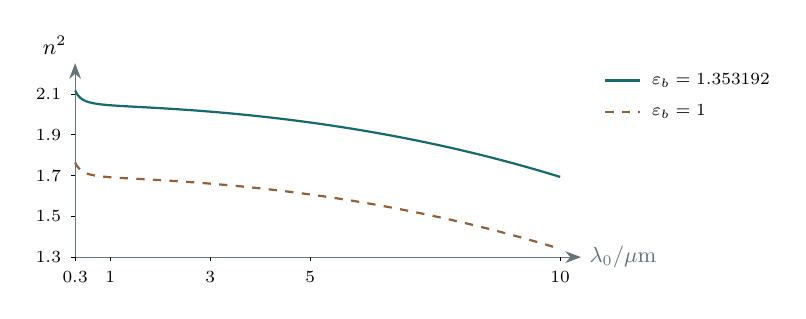
\begin{tikzpicture}[scale=.88,transform shape]
\draw[axis] (0,0)--(7.3,0) node[right] {$\lambda_0/{\rm \mu m}$};
\draw[axis] (0,0)--(0,2.8);
\node[above left] at (0,2.8) {$n^2$};
\draw[thin] (0.000000,0)--(0.000000,-0.06);\node[below,font=\scriptsize] at (0.000000,-0.08) {$ 0.3 $};
\draw[thin] (0.505155,0)--(0.505155,-0.06);\node[below,font=\scriptsize] at (0.505155,-0.08) {$ 1 $};
\draw[thin] (1.948454,0)--(1.948454,-0.06);\node[below,font=\scriptsize] at (1.948454,-0.08) {$ 3 $};
\draw[thin] (3.391753,0)--(3.391753,-0.06);\node[below,font=\scriptsize] at (3.391753,-0.08) {$ 5 $};
\draw[thin] (7.000000,0)--(7.000000,-0.06);\node[below,font=\scriptsize] at (7.000000,-0.08) {$ 10 $};
\draw[thin] (0,0.000000)--(-.06,0.000000);\node[left,font=\scriptsize] at (-.08,0.000000) {$ 1.3 $};
\draw[thin] (0,0.588235)--(-.06,0.588235);\node[left,font=\scriptsize] at (-.08,0.588235) {$ 1.5 $};
\draw[thin] (0,1.176471)--(-.06,1.176471);\node[left,font=\scriptsize] at (-.08,1.176471) {$ 1.7 $};
\draw[thin] (0,1.764706)--(-.06,1.764706);\node[left,font=\scriptsize] at (-.08,1.764706) {$ 1.9 $};
\draw[thin] (0,2.352941)--(-.06,2.352941);\node[left,font=\scriptsize] at (-.08,2.352941) {$ 2.1 $};
\draw[thick,color=accent] plot coordinates {(0.0000000,2.4045165) (0.0291667,2.3505972) (0.0583333,2.3143061) (0.0875000,2.2885761) (0.1166667,2.2695839) (0.1458333,2.2551020) (0.1750000,2.2437556) (0.2041667,2.2346572) (0.2333333,2.2272115) (0.2625000,2.2210065) (0.2916667,2.2157498) (0.3208333,2.2112287) (0.3500000,2.2072855) (0.3791667,2.2038012) (0.4083333,2.2006846) (0.4375000,2.1978649) (0.4666667,2.1952864) (0.4958333,2.1929046) (0.5250000,2.1906840) (0.5541667,2.1885956) (0.5833333,2.1866157) (0.6125000,2.1847248) (0.6416667,2.1829067) (0.6708333,2.1811478) (0.7000000,2.1794366) (0.7291667,2.1777636) (0.7583333,2.1761203) (0.7875000,2.1744999) (0.8166667,2.1728962) (0.8458333,2.1713040) (0.8750000,2.1697188) (0.9041667,2.1681365) (0.9333333,2.1665538) (0.9625000,2.1649675) (0.9916667,2.1633750) (1.0208333,2.1617740) (1.0500000,2.1601623) (1.0791667,2.1585381) (1.1083333,2.1568997) (1.1375000,2.1552456) (1.1666667,2.1535745) (1.1958333,2.1518851) (1.2250000,2.1501765) (1.2541667,2.1484476) (1.2833333,2.1466975) (1.3125000,2.1449254) (1.3416667,2.1431306) (1.3708333,2.1413124) (1.4000000,2.1394702) (1.4291667,2.1376034) (1.4583333,2.1357116) (1.4875000,2.1337942) (1.5166667,2.1318509) (1.5458333,2.1298811) (1.5750000,2.1278846) (1.6041667,2.1258609) (1.6333333,2.1238099) (1.6625000,2.1217311) (1.6916667,2.1196242) (1.7208333,2.1174891) (1.7500000,2.1153254) (1.7791667,2.1131330) (1.8083333,2.1109116) (1.8375000,2.1086611) (1.8666667,2.1063811) (1.8958333,2.1040716) (1.9250000,2.1017323) (1.9541667,2.0993632) (1.9833333,2.0969640) (2.0125000,2.0945345) (2.0416667,2.0920748) (2.0708333,2.0895845) (2.1000000,2.0870636) (2.1291667,2.0845120) (2.1583333,2.0819295) (2.1875000,2.0793160) (2.2166667,2.0766714) (2.2458333,2.0739956) (2.2750000,2.0712885) (2.3041667,2.0685500) (2.3333333,2.0657799) (2.3625000,2.0629783) (2.3916667,2.0601449) (2.4208333,2.0572798) (2.4500000,2.0543827) (2.4791667,2.0514537) (2.5083333,2.0484926) (2.5375000,2.0454993) (2.5666667,2.0424738) (2.5958333,2.0394160) (2.6250000,2.0363258) (2.6541667,2.0332031) (2.6833333,2.0300478) (2.7125000,2.0268599) (2.7416667,2.0236393) (2.7708333,2.0203859) (2.8000000,2.0170996) (2.8291667,2.0137803) (2.8583333,2.0104281) (2.8875000,2.0070427) (2.9166667,2.0036242) (2.9458333,2.0001724) (2.9750000,1.9966873) (3.0041667,1.9931688) (3.0333333,1.9896168) (3.0625000,1.9860313) (3.0916667,1.9824122) (3.1208333,1.9787594) (3.1500000,1.9750728) (3.1791667,1.9713524) (3.2083333,1.9675980) (3.2375000,1.9638097) (3.2666667,1.9599874) (3.2958333,1.9561309) (3.3250000,1.9522402) (3.3541667,1.9483152) (3.3833333,1.9443559) (3.4125000,1.9403621) (3.4416667,1.9363338) (3.4708333,1.9322710) (3.5000000,1.9281735) (3.5291667,1.9240413) (3.5583333,1.9198743) (3.5875000,1.9156724) (3.6166667,1.9114355) (3.6458333,1.9071636) (3.6750000,1.9028566) (3.7041667,1.8985144) (3.7333333,1.8941369) (3.7625000,1.8897241) (3.7916667,1.8852759) (3.8208333,1.8807921) (3.8500000,1.8762728) (3.8791667,1.8717178) (3.9083333,1.8671270) (3.9375000,1.8625005) (3.9666667,1.8578380) (3.9958333,1.8531395) (4.0250000,1.8484049) (4.0541667,1.8436341) (4.0833333,1.8388272) (4.1125000,1.8339838) (4.1416667,1.8291041) (4.1708333,1.8241878) (4.2000000,1.8192350) (4.2291667,1.8142455) (4.2583333,1.8092192) (4.2875000,1.8041560) (4.3166667,1.7990560) (4.3458333,1.7939188) (4.3750000,1.7887446) (4.4041667,1.7835331) (4.4333333,1.7782843) (4.4625000,1.7729981) (4.4916667,1.7676745) (4.5208333,1.7623132) (4.5500000,1.7569142) (4.5791667,1.7514775) (4.6083333,1.7460029) (4.6375000,1.7404903) (4.6666667,1.7349396) (4.6958333,1.7293508) (4.7250000,1.7237237) (4.7541667,1.7180582) (4.7833333,1.7123543) (4.8125000,1.7066118) (4.8416667,1.7008306) (4.8708333,1.6950107) (4.9000000,1.6891519) (4.9291667,1.6832541) (4.9583333,1.6773172) (4.9875000,1.6713411) (5.0166667,1.6653257) (5.0458333,1.6592709) (5.0750000,1.6531766) (5.1041667,1.6470427) (5.1333333,1.6408690) (5.1625000,1.6346555) (5.1916667,1.6284020) (5.2208333,1.6221085) (5.2500000,1.6157748) (5.2791667,1.6094007) (5.3083333,1.6029863) (5.3375000,1.5965314) (5.3666667,1.5900358) (5.3958333,1.5834994) (5.4250000,1.5769222) (5.4541667,1.5703039) (5.4833333,1.5636446) (5.5125000,1.5569440) (5.5416667,1.5502020) (5.5708333,1.5434185) (5.6000000,1.5365935) (5.6291667,1.5297267) (5.6583333,1.5228180) (5.6875000,1.5158674) (5.7166667,1.5088746) (5.7458333,1.5018396) (5.7750000,1.4947623) (5.8041667,1.4876424) (5.8333333,1.4804799) (5.8625000,1.4732746) (5.8916667,1.4660264) (5.9208333,1.4587352) (5.9500000,1.4514008) (5.9791667,1.4440232) (6.0083333,1.4366020) (6.0375000,1.4291373) (6.0666667,1.4216289) (6.0958333,1.4140765) (6.1250000,1.4064802) (6.1541667,1.3988398) (6.1833333,1.3911550) (6.2125000,1.3834258) (6.2416667,1.3756521) (6.2708333,1.3678336) (6.3000000,1.3599702) (6.3291667,1.3520618) (6.3583333,1.3441082) (6.3875000,1.3361093) (6.4166667,1.3280649) (6.4458333,1.3199749) (6.4750000,1.3118391) (6.5041667,1.3036573) (6.5333333,1.2954295) (6.5625000,1.2871553) (6.5916667,1.2788348) (6.6208333,1.2704677) (6.6500000,1.2620538) (6.6791667,1.2535930) (6.7083333,1.2450852) (6.7375000,1.2365301) (6.7666667,1.2279276) (6.7958333,1.2192776) (6.8250000,1.2105798) (6.8541667,1.2018341) (6.8833333,1.1930403) (6.9125000,1.1841982) (6.9416667,1.1753078) (6.9708333,1.1663687) (7.0000000,1.1573808)};
\draw[thick,color=accent] (7.65,2.55)--(8.15,2.55);\node[right,font=\scriptsize] at (8.2,2.55) {$\varepsilon_b=1.353192$};
\draw[thick,dashed,color=warm] plot coordinates {(0.0000000,1.3657172) (0.0291667,1.3117979) (0.0583333,1.2755068) (0.0875000,1.2497768) (0.1166667,1.2307846) (0.1458333,1.2163027) (0.1750000,1.2049563) (0.2041667,1.1958579) (0.2333333,1.1884122) (0.2625000,1.1822072) (0.2916667,1.1769505) (0.3208333,1.1724294) (0.3500000,1.1684862) (0.3791667,1.1650019) (0.4083333,1.1618853) (0.4375000,1.1590656) (0.4666667,1.1564871) (0.4958333,1.1541053) (0.5250000,1.1518847) (0.5541667,1.1497963) (0.5833333,1.1478164) (0.6125000,1.1459255) (0.6416667,1.1441074) (0.6708333,1.1423485) (0.7000000,1.1406373) (0.7291667,1.1389642) (0.7583333,1.1373210) (0.7875000,1.1357006) (0.8166667,1.1340969) (0.8458333,1.1325047) (0.8750000,1.1309195) (0.9041667,1.1293372) (0.9333333,1.1277544) (0.9625000,1.1261682) (0.9916667,1.1245757) (1.0208333,1.1229747) (1.0500000,1.1213630) (1.0791667,1.1197388) (1.1083333,1.1181004) (1.1375000,1.1164463) (1.1666667,1.1147752) (1.1958333,1.1130858) (1.2250000,1.1113772) (1.2541667,1.1096483) (1.2833333,1.1078981) (1.3125000,1.1061261) (1.3416667,1.1043313) (1.3708333,1.1025131) (1.4000000,1.1006709) (1.4291667,1.0988041) (1.4583333,1.0969123) (1.4875000,1.0949949) (1.5166667,1.0930516) (1.5458333,1.0910818) (1.5750000,1.0890853) (1.6041667,1.0870616) (1.6333333,1.0850106) (1.6625000,1.0829317) (1.6916667,1.0808249) (1.7208333,1.0786898) (1.7500000,1.0765261) (1.7791667,1.0743337) (1.8083333,1.0721123) (1.8375000,1.0698618) (1.8666667,1.0675818) (1.8958333,1.0652723) (1.9250000,1.0629330) (1.9541667,1.0605639) (1.9833333,1.0581647) (2.0125000,1.0557352) (2.0416667,1.0532755) (2.0708333,1.0507852) (2.1000000,1.0482643) (2.1291667,1.0457127) (2.1583333,1.0431302) (2.1875000,1.0405167) (2.2166667,1.0378721) (2.2458333,1.0351963) (2.2750000,1.0324892) (2.3041667,1.0297507) (2.3333333,1.0269806) (2.3625000,1.0241790) (2.3916667,1.0213456) (2.4208333,1.0184805) (2.4500000,1.0155834) (2.4791667,1.0126544) (2.5083333,1.0096933) (2.5375000,1.0067000) (2.5666667,1.0036745) (2.5958333,1.0006167) (2.6250000,0.9975265) (2.6541667,0.9944038) (2.6833333,0.9912485) (2.7125000,0.9880606) (2.7416667,0.9848400) (2.7708333,0.9815866) (2.8000000,0.9783003) (2.8291667,0.9749810) (2.8583333,0.9716288) (2.8875000,0.9682434) (2.9166667,0.9648249) (2.9458333,0.9613731) (2.9750000,0.9578880) (3.0041667,0.9543695) (3.0333333,0.9508175) (3.0625000,0.9472320) (3.0916667,0.9436129) (3.1208333,0.9399600) (3.1500000,0.9362735) (3.1791667,0.9325531) (3.2083333,0.9287987) (3.2375000,0.9250104) (3.2666667,0.9211881) (3.2958333,0.9173316) (3.3250000,0.9134409) (3.3541667,0.9095159) (3.3833333,0.9055566) (3.4125000,0.9015628) (3.4416667,0.8975345) (3.4708333,0.8934717) (3.5000000,0.8893742) (3.5291667,0.8852420) (3.5583333,0.8810750) (3.5875000,0.8768731) (3.6166667,0.8726362) (3.6458333,0.8683643) (3.6750000,0.8640573) (3.7041667,0.8597151) (3.7333333,0.8553376) (3.7625000,0.8509248) (3.7916667,0.8464766) (3.8208333,0.8419928) (3.8500000,0.8374735) (3.8791667,0.8329185) (3.9083333,0.8283277) (3.9375000,0.8237012) (3.9666667,0.8190387) (3.9958333,0.8143402) (4.0250000,0.8096056) (4.0541667,0.8048348) (4.0833333,0.8000278) (4.1125000,0.7951845) (4.1416667,0.7903048) (4.1708333,0.7853885) (4.2000000,0.7804357) (4.2291667,0.7754462) (4.2583333,0.7704199) (4.2875000,0.7653567) (4.3166667,0.7602567) (4.3458333,0.7551195) (4.3750000,0.7499453) (4.4041667,0.7447338) (4.4333333,0.7394850) (4.4625000,0.7341988) (4.4916667,0.7288752) (4.5208333,0.7235139) (4.5500000,0.7181149) (4.5791667,0.7126782) (4.6083333,0.7072036) (4.6375000,0.7016910) (4.6666667,0.6961403) (4.6958333,0.6905515) (4.7250000,0.6849244) (4.7541667,0.6792589) (4.7833333,0.6735550) (4.8125000,0.6678125) (4.8416667,0.6620313) (4.8708333,0.6562114) (4.9000000,0.6503526) (4.9291667,0.6444548) (4.9583333,0.6385179) (4.9875000,0.6325418) (5.0166667,0.6265264) (5.0458333,0.6204716) (5.0750000,0.6143773) (5.1041667,0.6082434) (5.1333333,0.6020697) (5.1625000,0.5958562) (5.1916667,0.5896027) (5.2208333,0.5833092) (5.2500000,0.5769755) (5.2791667,0.5706014) (5.3083333,0.5641870) (5.3375000,0.5577321) (5.3666667,0.5512365) (5.3958333,0.5447001) (5.4250000,0.5381229) (5.4541667,0.5315046) (5.4833333,0.5248453) (5.5125000,0.5181447) (5.5416667,0.5114027) (5.5708333,0.5046192) (5.6000000,0.4977942) (5.6291667,0.4909274) (5.6583333,0.4840187) (5.6875000,0.4770681) (5.7166667,0.4700753) (5.7458333,0.4630403) (5.7750000,0.4559630) (5.8041667,0.4488431) (5.8333333,0.4416806) (5.8625000,0.4344753) (5.8916667,0.4272271) (5.9208333,0.4199359) (5.9500000,0.4126015) (5.9791667,0.4052238) (6.0083333,0.3978027) (6.0375000,0.3903380) (6.0666667,0.3828296) (6.0958333,0.3752772) (6.1250000,0.3676809) (6.1541667,0.3600405) (6.1833333,0.3523557) (6.2125000,0.3446265) (6.2416667,0.3368528) (6.2708333,0.3290343) (6.3000000,0.3211709) (6.3291667,0.3132625) (6.3583333,0.3053089) (6.3875000,0.2973100) (6.4166667,0.2892656) (6.4458333,0.2811756) (6.4750000,0.2730398) (6.5041667,0.2648580) (6.5333333,0.2566301) (6.5625000,0.2483560) (6.5916667,0.2400355) (6.6208333,0.2316684) (6.6500000,0.2232545) (6.6791667,0.2147937) (6.7083333,0.2062859) (6.7375000,0.1977308) (6.7666667,0.1891283) (6.7958333,0.1804782) (6.8250000,0.1717805) (6.8541667,0.1630347) (6.8833333,0.1542410) (6.9125000,0.1453989) (6.9416667,0.1365085) (6.9708333,0.1275694) (7.0000000,0.1185815)};
\draw[thick,dashed,color=warm] (7.65,2.0999999999999996)--(8.15,2.0999999999999996);\node[right,font=\scriptsize] at (8.2,2.0999999999999996) {$\varepsilon_b=1$};
\end{tikzpicture}
\figcaption{解图光5.3D\quad 同一极点残数下背景使折射率平方整体平移0.353192}
\end{minipage}\end{center}
质量比是上述有效模型下的估计。实际晶体的离子集体振动和有效电荷可以用更多模态及相应权重表示，其他电子共振也进入完整高频响应；当前透明窗口内的折射率由这两个极点及常数背景共同描述。


\Needspace{13\baselineskip}

\pdfbookmark[2]{第 4 题 X射线色散及速度乘积}{q4}

\section*{第 4 题\quad X射线色散及速度乘积}\label{q:4}

在X射线频率远高于电子束缚共振频率、损耗可忽略的范围内，证明金属折射率满足$n^2=1-K\lambda_0^2$。对铜取原子序数29、相对原子质量63、密度$8.0\times10^3\,\mathrm{kg/m^3}$，估算$K$；再证明该模型内相速与群速的乘积为$c^2$。

\begin{center}\begin{minipage}{.98\linewidth}\centering
\begin{tikzpicture}[scale=.9,transform shape]
\draw[axis] (0.00000,0.00000)--(6.80000,0.00000);\draw[axis] (0.00000,-0.15000)--(0.00000,2.30000);\node[below right] at (6.80000,0.00000) {$\omega/\omega_p$};\node[above right] at (0.00000,2.30000) {$n^2$};\draw[traj] plot coordinates {(1.00000,0.00000) (1.03741,0.14164) (1.07482,0.26876) (1.11223,0.38326) (1.14964,0.48677) (1.18705,0.58064) (1.22446,0.66605) (1.26187,0.74397) (1.29928,0.81526) (1.33669,0.88064) (1.37410,0.94076) (1.41151,0.99617) (1.44892,1.04733) (1.48633,1.09469) (1.52374,1.13859) (1.56115,1.17938) (1.59856,1.21734) (1.63597,1.25273) (1.67338,1.28577) (1.71079,1.31666) (1.74820,1.34559) (1.78561,1.37273) (1.82302,1.39821) (1.86043,1.42217) (1.89784,1.44472) (1.93525,1.46598) (1.97266,1.48605) (2.01007,1.50500) (2.04748,1.52292) (2.08489,1.53989) (2.12230,1.55597) (2.15971,1.57122) (2.19712,1.58569) (2.23453,1.59945) (2.27194,1.61253) (2.30935,1.62498) (2.34676,1.63685) (2.38417,1.64815) (2.42158,1.65894) (2.45899,1.66924) (2.49640,1.67908) (2.53381,1.68848) (2.57122,1.69748) (2.60863,1.70610) (2.64604,1.71435) (2.68345,1.72226) (2.72086,1.72984) (2.75827,1.73712) (2.79568,1.74411) (2.83309,1.75082) (2.87050,1.75728) (2.90791,1.76348) (2.94532,1.76945) (2.98273,1.77520) (3.02014,1.78073) (3.05755,1.78607) (3.09496,1.79121) (3.13237,1.79616) (3.16978,1.80095) (3.20719,1.80556) (3.24460,1.81002) (3.28201,1.81433) (3.31942,1.81849) (3.35683,1.82251) (3.39424,1.82640) (3.43165,1.83017) (3.46906,1.83381) (3.50647,1.83734) (3.54388,1.84075) (3.58129,1.84406) (3.61871,1.84727) (3.65612,1.85038) (3.69353,1.85340) (3.73094,1.85632) (3.76835,1.85916) (3.80576,1.86191) (3.84317,1.86459) (3.88058,1.86719) (3.91799,1.86971) (3.95540,1.87216) (3.99281,1.87455) (4.03022,1.87687) (4.06763,1.87912) (4.10504,1.88131) (4.14245,1.88345) (4.17986,1.88553) (4.21727,1.88755) (4.25468,1.88952) (4.29209,1.89143) (4.32950,1.89330) (4.36691,1.89512) (4.40432,1.89690) (4.44173,1.89863) (4.47914,1.90031) (4.51655,1.90196) (4.55396,1.90356) (4.59137,1.90513) (4.62878,1.90665) (4.66619,1.90814) (4.70360,1.90960) (4.74101,1.91102) (4.77842,1.91241) (4.81583,1.91376) (4.85324,1.91509) (4.89065,1.91638) (4.92806,1.91765) (4.96547,1.91888) (5.00288,1.92009) (5.04029,1.92127) (5.07770,1.92243) (5.11511,1.92356) (5.15252,1.92467) (5.18993,1.92575) (5.22734,1.92681) (5.26475,1.92784) (5.30216,1.92886) (5.33957,1.92985) (5.37698,1.93082) (5.41439,1.93178) (5.45180,1.93271) (5.48921,1.93362) (5.52662,1.93452) (5.56403,1.93540) (5.60144,1.93626) (5.63885,1.93710) (5.67626,1.93793) (5.71367,1.93874) (5.75108,1.93953) (5.78849,1.94031) (5.82590,1.94107) (5.86331,1.94182) (5.90072,1.94256) (5.93813,1.94328) (5.97554,1.94399) (6.01295,1.94468) (6.05036,1.94537) (6.08777,1.94603) (6.12518,1.94669) (6.16259,1.94734) (6.20000,1.94797)};\draw[guide] (0.00000,2.00000)--(6.20000,2.00000);\node[left] at (0.00000,2.00000) {1};\node[below] at (1.00000,0.00000) {1};
\end{tikzpicture}
\figcaption{图光5.4\quad 高频传播区的折射率平方从零趋近1。}
\end{minipage}\end{center}

\Needspace{6\baselineskip}\subsection*{解答}


图光5.4的高频折射率由电子在电场中的惯性响应决定。对第$j$类束缚电子，$m_e(\omega_j^2-\omega^2)x_j=-eE$，偶极矩为$-ex_j$，所以各类电子对色散的贡献为
\[
n^2-1=\sum_j\frac{N_je^2}{\varepsilon_0m_e(\omega_j^2-\omega^2)}.
\]
在$\omega\gg\omega_j$并远离吸收边、损耗很小的范围，$1/(\omega_j^2-\omega^2)=-\omega^{-2}[1+O(\omega_j^2/\omega^2)]$。总电子数密度$N=\sum_jN_j$，把主导项相加有
\[
n^2=1-\frac{Ne^2}{\varepsilon_0m_e\omega^2}
=1-\frac{Ne^2}{4\pi^2\varepsilon_0m_ec^2}\lambda_0^2.
\]
因此$K=Ne^2/(4\pi^2\varepsilon_0m_ec^2)$，单位为$\mathrm{m^{-2}}$。电子的负电荷在位移与偶极矩中各出现一次，留下正的$e^2$；极化的负号由高频惯性分母给出。正离子响应也按电荷平方除以质量加权，其质量大，在该近似中贡献较小。

铜的原子数密度为$\rho N_A/(63\times10^{-3})$，高于全部束缚共振的模型每原子计29个电子，故
\[
N=\frac{29\rho N_A}{63\times10^{-3}}
\simeq2.22\times10^{30}\,\mathrm{m^{-3}},
\qquad
\boxed{K\simeq1.99\times10^{15}\,\mathrm{m^{-2}}}.
\]
用$N_A=6.02214\times10^{23}\,\mathrm{mol^{-1}}$、$e=1.60218\times10^{-19}\,\mathrm C$、$m_e=9.10938\times10^{-31}\,\mathrm{kg}$及$\varepsilon_0=8.85419\times10^{-12}\,\mathrm{F/m}$，得到$N=2.217677\times10^{30}\,\mathrm{m^{-3}}$、$K=1.986465\times10^{15}\,\mathrm{m^{-2}}$。在$.10\,\mathrm{nm}$处，$K\lambda_0^2=1.986465\times10^{-5}$，所以$n=.999990068$。解图光5.4C用$10^6(1-n)$显示这一小偏离；一阶式$1-n\simeq K\lambda_0^2/2$来自平方根展开。
\begin{center}\begin{minipage}{.98\linewidth}\centering
\begin{tikzpicture}[scale=.88,transform shape]
\draw[axis] (0,0.0)--(7.3,0.0) node[right] {$\lambda_0/{\rm nm}$};
\draw[axis] (0,0)--(0,2.8);
\node[above left] at (0,2.8) {$10^6(1-n)$};
\draw[thin] (0.000000,0.0)--(0.000000,-0.06);\node[below,font=\scriptsize] at (0.000000,-0.08) {$ 0.05 $};
\draw[thin] (2.333333,0.0)--(2.333333,-0.06);\node[below,font=\scriptsize] at (2.333333,-0.08) {$ 0.1 $};
\draw[thin] (4.666667,0.0)--(4.666667,-0.06);\node[below,font=\scriptsize] at (4.666667,-0.08) {$ 0.15 $};
\draw[thin] (7.000000,0.0)--(7.000000,-0.06);\node[below,font=\scriptsize] at (7.000000,-0.08) {$ 0.2 $};
\draw[thin] (0,0.000000)--(-.06,0.000000);\node[left,font=\scriptsize] at (-.08,0.000000) {$ 0 $};
\draw[thin] (0,0.595238)--(-.06,0.595238);\node[left,font=\scriptsize] at (-.08,0.595238) {$ 10 $};
\draw[thin] (0,1.190476)--(-.06,1.190476);\node[left,font=\scriptsize] at (-.08,1.190476) {$ 20 $};
\draw[thin] (0,1.785714)--(-.06,1.785714);\node[left,font=\scriptsize] at (-.08,1.785714) {$ 30 $};
\draw[thin] (0,2.380952)--(-.06,2.380952);\node[left,font=\scriptsize] at (-.08,2.380952) {$ 40 $};
\draw[thick,color=accent] plot coordinates {(0.0000000,0.1478027) (0.0291667,0.1515208) (0.0583333,0.1552852) (0.0875000,0.1590957) (0.1166667,0.1629525) (0.1458333,0.1668554) (0.1750000,0.1708045) (0.2041667,0.1747998) (0.2333333,0.1788413) (0.2625000,0.1829289) (0.2916667,0.1870628) (0.3208333,0.1912429) (0.3500000,0.1954691) (0.3791667,0.1997415) (0.4083333,0.2040602) (0.4375000,0.2084250) (0.4666667,0.2128360) (0.4958333,0.2172931) (0.5250000,0.2217965) (0.5541667,0.2263461) (0.5833333,0.2309418) (0.6125000,0.2355838) (0.6416667,0.2402719) (0.6708333,0.2450062) (0.7000000,0.2497867) (0.7291667,0.2546134) (0.7583333,0.2594863) (0.7875000,0.2644054) (0.8166667,0.2693706) (0.8458333,0.2743821) (0.8750000,0.2794397) (0.9041667,0.2845436) (0.9333333,0.2896936) (0.9625000,0.2948898) (0.9916667,0.3001322) (1.0208333,0.3054208) (1.0500000,0.3107555) (1.0791667,0.3161365) (1.1083333,0.3215636) (1.1375000,0.3270370) (1.1666667,0.3325565) (1.1958333,0.3381222) (1.2250000,0.3437341) (1.2541667,0.3493922) (1.2833333,0.3550965) (1.3125000,0.3608470) (1.3416667,0.3666437) (1.3708333,0.3724865) (1.4000000,0.3783756) (1.4291667,0.3843108) (1.4583333,0.3902922) (1.4875000,0.3963198) (1.5166667,0.4023936) (1.5458333,0.4085136) (1.5750000,0.4146798) (1.6041667,0.4208921) (1.6333333,0.4271507) (1.6625000,0.4334554) (1.6916667,0.4398064) (1.7208333,0.4462035) (1.7500000,0.4526468) (1.7791667,0.4591363) (1.8083333,0.4656720) (1.8375000,0.4722539) (1.8666667,0.4788820) (1.8958333,0.4855562) (1.9250000,0.4922767) (1.9541667,0.4990433) (1.9833333,0.5058561) (2.0125000,0.5127152) (2.0416667,0.5196204) (2.0708333,0.5265718) (2.1000000,0.5335693) (2.1291667,0.5406131) (2.1583333,0.5477031) (2.1875000,0.5548392) (2.2166667,0.5620216) (2.2458333,0.5692501) (2.2750000,0.5765248) (2.3041667,0.5838458) (2.3333333,0.5912129) (2.3625000,0.5986262) (2.3916667,0.6060856) (2.4208333,0.6135913) (2.4500000,0.6211432) (2.4791667,0.6287412) (2.5083333,0.6363855) (2.5375000,0.6440759) (2.5666667,0.6518125) (2.5958333,0.6595953) (2.6250000,0.6674243) (2.6541667,0.6752995) (2.6833333,0.6832209) (2.7125000,0.6911885) (2.7416667,0.6992022) (2.7708333,0.7072622) (2.8000000,0.7153683) (2.8291667,0.7235206) (2.8583333,0.7317192) (2.8875000,0.7399639) (2.9166667,0.7482548) (2.9458333,0.7565919) (2.9750000,0.7649751) (3.0041667,0.7734046) (3.0333333,0.7818803) (3.0625000,0.7904021) (3.0916667,0.7989701) (3.1208333,0.8075844) (3.1500000,0.8162448) (3.1791667,0.8249514) (3.2083333,0.8337042) (3.2375000,0.8425032) (3.2666667,0.8513484) (3.2958333,0.8602397) (3.3250000,0.8691773) (3.3541667,0.8781611) (3.3833333,0.8871910) (3.4125000,0.8962671) (3.4416667,0.9053895) (3.4708333,0.9145580) (3.5000000,0.9237727) (3.5291667,0.9330336) (3.5583333,0.9423407) (3.5875000,0.9516939) (3.6166667,0.9610934) (3.6458333,0.9705390) (3.6750000,0.9800309) (3.7041667,0.9895689) (3.7333333,0.9991532) (3.7625000,1.0087836) (3.7916667,1.0184602) (3.8208333,1.0281830) (3.8500000,1.0379520) (3.8791667,1.0477672) (3.9083333,1.0576285) (3.9375000,1.0675361) (3.9666667,1.0774898) (3.9958333,1.0874898) (4.0250000,1.0975359) (4.0541667,1.1076282) (4.0833333,1.1177668) (4.1125000,1.1279515) (4.1416667,1.1381824) (4.1708333,1.1484595) (4.2000000,1.1587827) (4.2291667,1.1691522) (4.2583333,1.1795679) (4.2875000,1.1900297) (4.3166667,1.2005378) (4.3458333,1.2110920) (4.3750000,1.2216924) (4.4041667,1.2323390) (4.4333333,1.2430318) (4.4625000,1.2537708) (4.4916667,1.2645560) (4.5208333,1.2753874) (4.5500000,1.2862650) (4.5791667,1.2971888) (4.6083333,1.3081587) (4.6375000,1.3191749) (4.6666667,1.3302372) (4.6958333,1.3413457) (4.7250000,1.3525004) (4.7541667,1.3637014) (4.7833333,1.3749485) (4.8125000,1.3862418) (4.8416667,1.3975812) (4.8708333,1.4089669) (4.9000000,1.4203988) (4.9291667,1.4318769) (4.9583333,1.4434011) (4.9875000,1.4549715) (5.0166667,1.4665882) (5.0458333,1.4782510) (5.0750000,1.4899600) (5.1041667,1.5017152) (5.1333333,1.5135166) (5.1625000,1.5253642) (5.1916667,1.5372580) (5.2208333,1.5491980) (5.2500000,1.5611842) (5.2791667,1.5732165) (5.3083333,1.5852951) (5.3375000,1.5974198) (5.3666667,1.6095908) (5.3958333,1.6218079) (5.4250000,1.6340712) (5.4541667,1.6463807) (5.4833333,1.6587365) (5.5125000,1.6711384) (5.5416667,1.6835864) (5.5708333,1.6960807) (5.6000000,1.7086212) (5.6291667,1.7212079) (5.6583333,1.7338407) (5.6875000,1.7465198) (5.7166667,1.7592450) (5.7458333,1.7720165) (5.7750000,1.7848341) (5.8041667,1.7976979) (5.8333333,1.8106079) (5.8625000,1.8235641) (5.8916667,1.8365665) (5.9208333,1.8496151) (5.9500000,1.8627099) (5.9791667,1.8758509) (6.0083333,1.8890381) (6.0375000,1.9022714) (6.0666667,1.9155510) (6.0958333,1.9288767) (6.1250000,1.9422487) (6.1541667,1.9556668) (6.1833333,1.9691311) (6.2125000,1.9826416) (6.2416667,1.9961984) (6.2708333,2.0098013) (6.3000000,2.0234504) (6.3291667,2.0371456) (6.3583333,2.0508871) (6.3875000,2.0646748) (6.4166667,2.0785087) (6.4458333,2.0923887) (6.4750000,2.1063150) (6.5041667,2.1202874) (6.5333333,2.1343061) (6.5625000,2.1483709) (6.5916667,2.1624820) (6.6208333,2.1766392) (6.6500000,2.1908426) (6.6791667,2.2050922) (6.7083333,2.2193880) (6.7375000,2.2337300) (6.7666667,2.2481182) (6.7958333,2.2625526) (6.8250000,2.2770331) (6.8541667,2.2915599) (6.8833333,2.3061329) (6.9125000,2.3207520) (6.9416667,2.3354174) (6.9708333,2.3501289) (7.0000000,2.3648867)};
\end{tikzpicture}
\figcaption{解图光5.4C\quad 硬X射线高频模型的折射率小偏离}
\end{minipage}\end{center}
令$\omega_p^2=Ne^2/(\varepsilon_0m_e)=4\pi^2c^2K$，结合$k=n\omega/c$把波长色散写成
\[
c^2k^2=\omega^2-\omega_p^2,\quad
\omega=\sqrt{c^2k^2+\omega_p^2}.
\]
在传播分支$\omega>\omega_p$上取$k>0$，解图光5.4A给出这条有纵轴截距的色散线。通过同一点$P$的原点割线与局部切线分别给相速和群速：
\[
v_p=\frac{\omega}{k}=\frac cn,\qquad
v_g=\frac{\dd\omega}{\dd k}=\frac{c^2k}{\omega}=cn,
\]
\[
\boxed{v_pv_g=c^2}.
\]
用介质内波长还可直接求群速：$\lambda_m=\lambda_0/n$、$1/\lambda_0=\sqrt{(1/\lambda_m)^2+K}$，沿$1/\lambda_m$求导，得到
\[
v_g=\frac{\dd(c/\lambda_0)}{\dd(1/\lambda_m)}
=\frac{c/\lambda_m}{\sqrt{\lambda_m^{-2}+K}}
=\frac{cn}{\sqrt{n^2+K\lambda_0^2}}=cn.
\]这里用真空波长写介质参数，再沿内部波数求导，转换由$\lambda_m=\lambda_0/n$给出。
\begin{center}\begin{minipage}{.98\linewidth}\centering
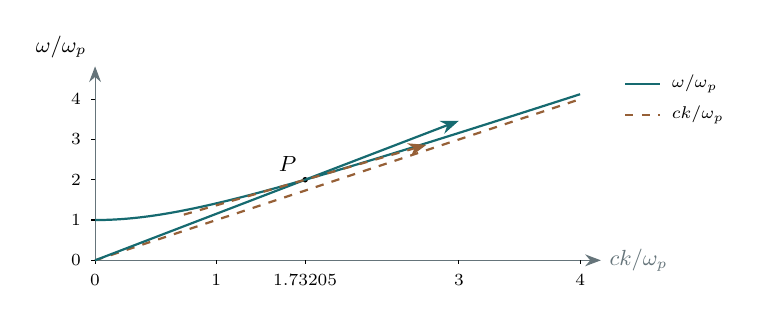
\begin{tikzpicture}[scale=.88,transform shape]
\draw[axis] (0,0.0)--(7.3,0.0) node[right] {$ck/\omega_p$};
\draw[axis] (0,0)--(0,2.8);
\node[above left] at (0,2.8) {$\omega/\omega_p$};
\draw[thin] (0.000000,0.0)--(0.000000,-0.06);\node[below,font=\scriptsize] at (0.000000,-0.08) {$ 0 $};
\draw[thin] (1.750000,0.0)--(1.750000,-0.06);\node[below,font=\scriptsize] at (1.750000,-0.08) {$ 1 $};
\draw[thin] (3.031089,0.0)--(3.031089,-0.06);\node[below,font=\scriptsize] at (3.031089,-0.08) {$ 1.73205 $};
\draw[thin] (5.250000,0.0)--(5.250000,-0.06);\node[below,font=\scriptsize] at (5.250000,-0.08) {$ 3 $};
\draw[thin] (7.000000,0.0)--(7.000000,-0.06);\node[below,font=\scriptsize] at (7.000000,-0.08) {$ 4 $};
\draw[thin] (0,0.000000)--(-.06,0.000000);\node[left,font=\scriptsize] at (-.08,0.000000) {$ 0 $};
\draw[thin] (0,0.581395)--(-.06,0.581395);\node[left,font=\scriptsize] at (-.08,0.581395) {$ 1 $};
\draw[thin] (0,1.162791)--(-.06,1.162791);\node[left,font=\scriptsize] at (-.08,1.162791) {$ 2 $};
\draw[thin] (0,1.744186)--(-.06,1.744186);\node[left,font=\scriptsize] at (-.08,1.744186) {$ 3 $};
\draw[thin] (0,2.325581)--(-.06,2.325581);\node[left,font=\scriptsize] at (-.08,2.325581) {$ 4 $};
\draw[thick,color=accent] plot coordinates {(0.0000000,0.5813953) (0.0291667,0.5814761) (0.0583333,0.5817183) (0.0875000,0.5821216) (0.1166667,0.5826859) (0.1458333,0.5834106) (0.1750000,0.5842951) (0.2041667,0.5853387) (0.2333333,0.5865405) (0.2625000,0.5878997) (0.2916667,0.5894150) (0.3208333,0.5910853) (0.3500000,0.5929092) (0.3791667,0.5948855) (0.4083333,0.5970125) (0.4375000,0.5992886) (0.4666667,0.6017122) (0.4958333,0.6042815) (0.5250000,0.6069946) (0.5541667,0.6098496) (0.5833333,0.6128445) (0.6125000,0.6159773) (0.6416667,0.6192459) (0.6708333,0.6226482) (0.7000000,0.6261820) (0.7291667,0.6298450) (0.7583333,0.6336350) (0.7875000,0.6375498) (0.8166667,0.6415870) (0.8458333,0.6457445) (0.8750000,0.6500198) (0.9041667,0.6544106) (0.9333333,0.6589147) (0.9625000,0.6635298) (0.9916667,0.6682535) (1.0208333,0.6730835) (1.0500000,0.6780177) (1.0791667,0.6830536) (1.1083333,0.6881892) (1.1375000,0.6934221) (1.1666667,0.6987502) (1.1958333,0.7041714) (1.2250000,0.7096835) (1.2541667,0.7152843) (1.2833333,0.7209719) (1.3125000,0.7267442) (1.3416667,0.7325992) (1.3708333,0.7385348) (1.4000000,0.7445493) (1.4291667,0.7506407) (1.4583333,0.7568071) (1.4875000,0.7630468) (1.5166667,0.7693579) (1.5458333,0.7757387) (1.5750000,0.7821874) (1.6041667,0.7887025) (1.6333333,0.7952823) (1.6625000,0.8019252) (1.6916667,0.8086297) (1.7208333,0.8153942) (1.7500000,0.8222172) (1.7791667,0.8290973) (1.8083333,0.8360331) (1.8375000,0.8430233) (1.8666667,0.8500664) (1.8958333,0.8571611) (1.9250000,0.8643063) (1.9541667,0.8715007) (1.9833333,0.8787429) (2.0125000,0.8860320) (2.0416667,0.8933667) (2.0708333,0.9007459) (2.1000000,0.9081686) (2.1291667,0.9156336) (2.1583333,0.9231400) (2.1875000,0.9306867) (2.2166667,0.9382727) (2.2458333,0.9458973) (2.2750000,0.9535593) (2.3041667,0.9612579) (2.3333333,0.9689922) (2.3625000,0.9767615) (2.3916667,0.9845648) (2.4208333,0.9924013) (2.4500000,1.0002704) (2.4791667,1.0081711) (2.5083333,1.0161028) (2.5375000,1.0240648) (2.5666667,1.0320564) (2.5958333,1.0400768) (2.6250000,1.0481254) (2.6541667,1.0562016) (2.6833333,1.0643047) (2.7125000,1.0724341) (2.7416667,1.0805893) (2.7708333,1.0887696) (2.8000000,1.0969746) (2.8291667,1.1052035) (2.8583333,1.1134560) (2.8875000,1.1217315) (2.9166667,1.1300294) (2.9458333,1.1383494) (2.9750000,1.1466909) (3.0041667,1.1550534) (3.0333333,1.1634365) (3.0625000,1.1718398) (3.0916667,1.1802628) (3.1208333,1.1887051) (3.1500000,1.1971663) (3.1791667,1.2056460) (3.2083333,1.2141438) (3.2375000,1.2226594) (3.2666667,1.2311923) (3.2958333,1.2397422) (3.3250000,1.2483088) (3.3541667,1.2568916) (3.3833333,1.2654905) (3.4125000,1.2741051) (3.4416667,1.2827349) (3.4708333,1.2913799) (3.5000000,1.3000395) (3.5291667,1.3087136) (3.5583333,1.3174019) (3.5875000,1.3261040) (3.6166667,1.3348198) (3.6458333,1.3435489) (3.6750000,1.3522911) (3.7041667,1.3610461) (3.7333333,1.3698137) (3.7625000,1.3785937) (3.7916667,1.3873858) (3.8208333,1.3961897) (3.8500000,1.4050053) (3.8791667,1.4138324) (3.9083333,1.4226707) (3.9375000,1.4315200) (3.9666667,1.4403802) (3.9958333,1.4492509) (4.0250000,1.4581321) (4.0541667,1.4670235) (4.0833333,1.4759250) (4.1125000,1.4848364) (4.1416667,1.4937574) (4.1708333,1.5026880) (4.2000000,1.5116279) (4.2291667,1.5205770) (4.2583333,1.5295352) (4.2875000,1.5385022) (4.3166667,1.5474779) (4.3458333,1.5564622) (4.3750000,1.5654549) (4.4041667,1.5744559) (4.4333333,1.5834650) (4.4625000,1.5924821) (4.4916667,1.6015070) (4.5208333,1.6105397) (4.5500000,1.6195800) (4.5791667,1.6286278) (4.6083333,1.6376829) (4.6375000,1.6467452) (4.6666667,1.6558147) (4.6958333,1.6648911) (4.7250000,1.6739744) (4.7541667,1.6830645) (4.7833333,1.6921612) (4.8125000,1.7012645) (4.8416667,1.7103743) (4.8708333,1.7194903) (4.9000000,1.7286126) (4.9291667,1.7377411) (4.9583333,1.7468756) (4.9875000,1.7560161) (5.0166667,1.7651624) (5.0458333,1.7743145) (5.0750000,1.7834723) (5.1041667,1.7926357) (5.1333333,1.8018045) (5.1625000,1.8109789) (5.1916667,1.8201585) (5.2208333,1.8293434) (5.2500000,1.8385335) (5.2791667,1.8477287) (5.3083333,1.8569290) (5.3375000,1.8661342) (5.3666667,1.8753442) (5.3958333,1.8845591) (5.4250000,1.8937788) (5.4541667,1.9030031) (5.4833333,1.9122320) (5.5125000,1.9214654) (5.5416667,1.9307034) (5.5708333,1.9399457) (5.6000000,1.9491924) (5.6291667,1.9584434) (5.6583333,1.9676986) (5.6875000,1.9769579) (5.7166667,1.9862214) (5.7458333,1.9954889) (5.7750000,2.0047604) (5.8041667,2.0140359) (5.8333333,2.0233152) (5.8625000,2.0325984) (5.8916667,2.0418853) (5.9208333,2.0511760) (5.9500000,2.0604704) (5.9791667,2.0697683) (6.0083333,2.0790699) (6.0375000,2.0883750) (6.0666667,2.0976836) (6.0958333,2.1069956) (6.1250000,2.1163110) (6.1541667,2.1256298) (6.1833333,2.1349518) (6.2125000,2.1442772) (6.2416667,2.1536057) (6.2708333,2.1629374) (6.3000000,2.1722723) (6.3291667,2.1816102) (6.3583333,2.1909513) (6.3875000,2.2002953) (6.4166667,2.2096423) (6.4458333,2.2189922) (6.4750000,2.2283451) (6.5041667,2.2377008) (6.5333333,2.2470594) (6.5625000,2.2564207) (6.5916667,2.2657849) (6.6208333,2.2751517) (6.6500000,2.2845212) (6.6791667,2.2938934) (6.7083333,2.3032683) (6.7375000,2.3126457) (6.7666667,2.3220257) (6.7958333,2.3314082) (6.8250000,2.3407933) (6.8541667,2.3501808) (6.8833333,2.3595707) (6.9125000,2.3689631) (6.9416667,2.3783579) (6.9708333,2.3877550) (7.0000000,2.3971544)};
\draw[thick,color=accent] (7.65,2.55)--(8.15,2.55);\node[right,font=\scriptsize] at (8.2,2.55) {$\omega/\omega_p$};
\draw[thick,dashed,color=warm] plot coordinates {(0.0000000,0.0000000) (0.0291667,0.0096899) (0.0583333,0.0193798) (0.0875000,0.0290698) (0.1166667,0.0387597) (0.1458333,0.0484496) (0.1750000,0.0581395) (0.2041667,0.0678295) (0.2333333,0.0775194) (0.2625000,0.0872093) (0.2916667,0.0968992) (0.3208333,0.1065891) (0.3500000,0.1162791) (0.3791667,0.1259690) (0.4083333,0.1356589) (0.4375000,0.1453488) (0.4666667,0.1550388) (0.4958333,0.1647287) (0.5250000,0.1744186) (0.5541667,0.1841085) (0.5833333,0.1937984) (0.6125000,0.2034884) (0.6416667,0.2131783) (0.6708333,0.2228682) (0.7000000,0.2325581) (0.7291667,0.2422481) (0.7583333,0.2519380) (0.7875000,0.2616279) (0.8166667,0.2713178) (0.8458333,0.2810078) (0.8750000,0.2906977) (0.9041667,0.3003876) (0.9333333,0.3100775) (0.9625000,0.3197674) (0.9916667,0.3294574) (1.0208333,0.3391473) (1.0500000,0.3488372) (1.0791667,0.3585271) (1.1083333,0.3682171) (1.1375000,0.3779070) (1.1666667,0.3875969) (1.1958333,0.3972868) (1.2250000,0.4069767) (1.2541667,0.4166667) (1.2833333,0.4263566) (1.3125000,0.4360465) (1.3416667,0.4457364) (1.3708333,0.4554264) (1.4000000,0.4651163) (1.4291667,0.4748062) (1.4583333,0.4844961) (1.4875000,0.4941860) (1.5166667,0.5038760) (1.5458333,0.5135659) (1.5750000,0.5232558) (1.6041667,0.5329457) (1.6333333,0.5426357) (1.6625000,0.5523256) (1.6916667,0.5620155) (1.7208333,0.5717054) (1.7500000,0.5813953) (1.7791667,0.5910853) (1.8083333,0.6007752) (1.8375000,0.6104651) (1.8666667,0.6201550) (1.8958333,0.6298450) (1.9250000,0.6395349) (1.9541667,0.6492248) (1.9833333,0.6589147) (2.0125000,0.6686047) (2.0416667,0.6782946) (2.0708333,0.6879845) (2.1000000,0.6976744) (2.1291667,0.7073643) (2.1583333,0.7170543) (2.1875000,0.7267442) (2.2166667,0.7364341) (2.2458333,0.7461240) (2.2750000,0.7558140) (2.3041667,0.7655039) (2.3333333,0.7751938) (2.3625000,0.7848837) (2.3916667,0.7945736) (2.4208333,0.8042636) (2.4500000,0.8139535) (2.4791667,0.8236434) (2.5083333,0.8333333) (2.5375000,0.8430233) (2.5666667,0.8527132) (2.5958333,0.8624031) (2.6250000,0.8720930) (2.6541667,0.8817829) (2.6833333,0.8914729) (2.7125000,0.9011628) (2.7416667,0.9108527) (2.7708333,0.9205426) (2.8000000,0.9302326) (2.8291667,0.9399225) (2.8583333,0.9496124) (2.8875000,0.9593023) (2.9166667,0.9689922) (2.9458333,0.9786822) (2.9750000,0.9883721) (3.0041667,0.9980620) (3.0333333,1.0077519) (3.0625000,1.0174419) (3.0916667,1.0271318) (3.1208333,1.0368217) (3.1500000,1.0465116) (3.1791667,1.0562016) (3.2083333,1.0658915) (3.2375000,1.0755814) (3.2666667,1.0852713) (3.2958333,1.0949612) (3.3250000,1.1046512) (3.3541667,1.1143411) (3.3833333,1.1240310) (3.4125000,1.1337209) (3.4416667,1.1434109) (3.4708333,1.1531008) (3.5000000,1.1627907) (3.5291667,1.1724806) (3.5583333,1.1821705) (3.5875000,1.1918605) (3.6166667,1.2015504) (3.6458333,1.2112403) (3.6750000,1.2209302) (3.7041667,1.2306202) (3.7333333,1.2403101) (3.7625000,1.2500000) (3.7916667,1.2596899) (3.8208333,1.2693798) (3.8500000,1.2790698) (3.8791667,1.2887597) (3.9083333,1.2984496) (3.9375000,1.3081395) (3.9666667,1.3178295) (3.9958333,1.3275194) (4.0250000,1.3372093) (4.0541667,1.3468992) (4.0833333,1.3565891) (4.1125000,1.3662791) (4.1416667,1.3759690) (4.1708333,1.3856589) (4.2000000,1.3953488) (4.2291667,1.4050388) (4.2583333,1.4147287) (4.2875000,1.4244186) (4.3166667,1.4341085) (4.3458333,1.4437984) (4.3750000,1.4534884) (4.4041667,1.4631783) (4.4333333,1.4728682) (4.4625000,1.4825581) (4.4916667,1.4922481) (4.5208333,1.5019380) (4.5500000,1.5116279) (4.5791667,1.5213178) (4.6083333,1.5310078) (4.6375000,1.5406977) (4.6666667,1.5503876) (4.6958333,1.5600775) (4.7250000,1.5697674) (4.7541667,1.5794574) (4.7833333,1.5891473) (4.8125000,1.5988372) (4.8416667,1.6085271) (4.8708333,1.6182171) (4.9000000,1.6279070) (4.9291667,1.6375969) (4.9583333,1.6472868) (4.9875000,1.6569767) (5.0166667,1.6666667) (5.0458333,1.6763566) (5.0750000,1.6860465) (5.1041667,1.6957364) (5.1333333,1.7054264) (5.1625000,1.7151163) (5.1916667,1.7248062) (5.2208333,1.7344961) (5.2500000,1.7441860) (5.2791667,1.7538760) (5.3083333,1.7635659) (5.3375000,1.7732558) (5.3666667,1.7829457) (5.3958333,1.7926357) (5.4250000,1.8023256) (5.4541667,1.8120155) (5.4833333,1.8217054) (5.5125000,1.8313953) (5.5416667,1.8410853) (5.5708333,1.8507752) (5.6000000,1.8604651) (5.6291667,1.8701550) (5.6583333,1.8798450) (5.6875000,1.8895349) (5.7166667,1.8992248) (5.7458333,1.9089147) (5.7750000,1.9186047) (5.8041667,1.9282946) (5.8333333,1.9379845) (5.8625000,1.9476744) (5.8916667,1.9573643) (5.9208333,1.9670543) (5.9500000,1.9767442) (5.9791667,1.9864341) (6.0083333,1.9961240) (6.0375000,2.0058140) (6.0666667,2.0155039) (6.0958333,2.0251938) (6.1250000,2.0348837) (6.1541667,2.0445736) (6.1833333,2.0542636) (6.2125000,2.0639535) (6.2416667,2.0736434) (6.2708333,2.0833333) (6.3000000,2.0930233) (6.3291667,2.1027132) (6.3583333,2.1124031) (6.3875000,2.1220930) (6.4166667,2.1317829) (6.4458333,2.1414729) (6.4750000,2.1511628) (6.5041667,2.1608527) (6.5333333,2.1705426) (6.5625000,2.1802326) (6.5916667,2.1899225) (6.6208333,2.1996124) (6.6500000,2.2093023) (6.6791667,2.2189922) (6.7083333,2.2286822) (6.7375000,2.2383721) (6.7666667,2.2480620) (6.7958333,2.2577519) (6.8250000,2.2674419) (6.8541667,2.2771318) (6.8833333,2.2868217) (6.9125000,2.2965116) (6.9416667,2.3062016) (6.9708333,2.3158915) (7.0000000,2.3255814)};
\draw[thick,dashed,color=warm] (7.65,2.0999999999999996)--(8.15,2.0999999999999996);\node[right,font=\scriptsize] at (8.2,2.0999999999999996) {$ck/\omega_p$};
\fill (3.0310889,1.1627907) circle(.04);\node[above left] at (3.0310889,1.1627907) {$P$};
\draw[motion] (0,0)--(5.2500000,2.0140126);
\draw[force,dashed] (1.2810889,0.6592876)--(4.7810889,1.6662938);
\end{tikzpicture}
\figcaption{解图光5.4A\quad 高频电子平方型色散与真空光线}
\end{minipage}\end{center}
解图光5.4B在传播区画出$v_p/c=1/n$与$v_g/c=n$。$0<n<1$时相位面较快、窄带包络较慢，二者相乘为1；高频时$n\to1$，两速度均趋于$c$。相位速度描述周期相位面，能量包络按$cn$传播，信号前沿由完整因果响应确定。
\begin{center}\begin{minipage}{.98\linewidth}\centering
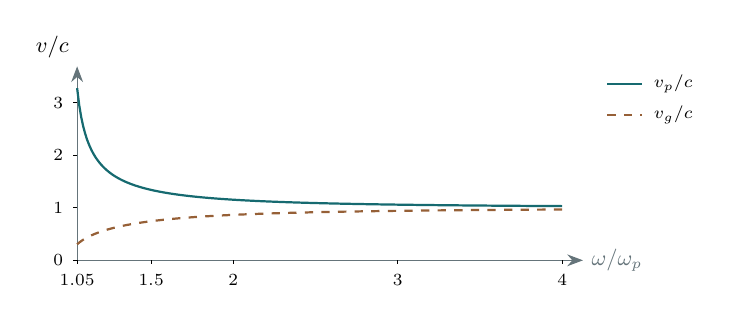
\begin{tikzpicture}[scale=.88,transform shape]
\draw[axis] (0,0.0)--(7.3,0.0) node[right] {$\omega/\omega_p$};
\draw[axis] (0,0)--(0,2.8);
\node[above left] at (0,2.8) {$v/c$};
\draw[thin] (0.000000,0.0)--(0.000000,-0.06);\node[below,font=\scriptsize] at (0.000000,-0.08) {$ 1.05 $};
\draw[thin] (1.067797,0.0)--(1.067797,-0.06);\node[below,font=\scriptsize] at (1.067797,-0.08) {$ 1.5 $};
\draw[thin] (2.254237,0.0)--(2.254237,-0.06);\node[below,font=\scriptsize] at (2.254237,-0.08) {$ 2 $};
\draw[thin] (4.627119,0.0)--(4.627119,-0.06);\node[below,font=\scriptsize] at (4.627119,-0.08) {$ 3 $};
\draw[thin] (7.000000,0.0)--(7.000000,-0.06);\node[below,font=\scriptsize] at (7.000000,-0.08) {$ 4 $};
\draw[thin] (0,0.000000)--(-.06,0.000000);\node[left,font=\scriptsize] at (-.08,0.000000) {$ 0 $};
\draw[thin] (0,0.757576)--(-.06,0.757576);\node[left,font=\scriptsize] at (-.08,0.757576) {$ 1 $};
\draw[thin] (0,1.515152)--(-.06,1.515152);\node[left,font=\scriptsize] at (-.08,1.515152) {$ 2 $};
\draw[thin] (0,2.272727)--(-.06,2.272727);\node[left,font=\scriptsize] at (-.08,2.272727) {$ 3 $};
\draw[thick,color=accent] plot coordinates {(0.0000000,2.4845826) (0.0291667,2.2453282) (0.0583333,2.0695686) (0.0875000,1.9337933) (0.1166667,1.8250859) (0.1458333,1.7356883) (0.1750000,1.6606246) (0.2041667,1.5965389) (0.2333333,1.5410752) (0.2625000,1.4925254) (0.2916667,1.4496170) (0.3208333,1.4113804) (0.3500000,1.3770623) (0.3791667,1.3460676) (0.4083333,1.3179190) (0.4375000,1.2922291) (0.4666667,1.2686793) (0.4958333,1.2470055) (0.5250000,1.2269862) (0.5541667,1.2084345) (0.5833333,1.1911912) (0.6125000,1.1751199) (0.6416667,1.1601029) (0.6708333,1.1460383) (0.7000000,1.1328369) (0.7291667,1.1204208) (0.7583333,1.1087212) (0.7875000,1.0976774) (0.8166667,1.0872355) (0.8458333,1.0773474) (0.8750000,1.0679700) (0.9041667,1.0590648) (0.9333333,1.0505970) (0.9625000,1.0425353) (0.9916667,1.0348513) (1.0208333,1.0275193) (1.0500000,1.0205157) (1.0791667,1.0138193) (1.1083333,1.0074104) (1.1375000,1.0012712) (1.1666667,0.9953852) (1.1958333,0.9897374) (1.2250000,0.9843138) (1.2541667,0.9791015) (1.2833333,0.9740887) (1.3125000,0.9692644) (1.3416667,0.9646184) (1.3708333,0.9601413) (1.4000000,0.9558241) (1.4291667,0.9516587) (1.4583333,0.9476375) (1.4875000,0.9437533) (1.5166667,0.9399994) (1.5458333,0.9363696) (1.5750000,0.9328580) (1.6041667,0.9294592) (1.6333333,0.9261679) (1.6625000,0.9229794) (1.6916667,0.9198890) (1.7208333,0.9168924) (1.7500000,0.9139857) (1.7791667,0.9111650) (1.8083333,0.9084266) (1.8375000,0.9057672) (1.8666667,0.9031836) (1.8958333,0.9006726) (1.9250000,0.8982315) (1.9541667,0.8958574) (1.9833333,0.8935477) (2.0125000,0.8913000) (2.0416667,0.8891120) (2.0708333,0.8869814) (2.1000000,0.8849061) (2.1291667,0.8828840) (2.1583333,0.8809133) (2.1875000,0.8789921) (2.2166667,0.8771187) (2.2458333,0.8752913) (2.2750000,0.8735085) (2.3041667,0.8717686) (2.3333333,0.8700703) (2.3625000,0.8684122) (2.3916667,0.8667928) (2.4208333,0.8652110) (2.4500000,0.8636655) (2.4791667,0.8621552) (2.5083333,0.8606789) (2.5375000,0.8592356) (2.5666667,0.8578243) (2.5958333,0.8564439) (2.6250000,0.8550935) (2.6541667,0.8537722) (2.6833333,0.8524792) (2.7125000,0.8512135) (2.7416667,0.8499745) (2.7708333,0.8487612) (2.8000000,0.8475730) (2.8291667,0.8464091) (2.8583333,0.8452689) (2.8875000,0.8441517) (2.9166667,0.8430568) (2.9458333,0.8419836) (2.9750000,0.8409316) (3.0041667,0.8399001) (3.0333333,0.8388886) (3.0625000,0.8378965) (3.0916667,0.8369234) (3.1208333,0.8359687) (3.1500000,0.8350320) (3.1791667,0.8341127) (3.2083333,0.8332105) (3.2375000,0.8323249) (3.2666667,0.8314555) (3.2958333,0.8306018) (3.3250000,0.8297635) (3.3541667,0.8289402) (3.3833333,0.8281316) (3.4125000,0.8273372) (3.4416667,0.8265567) (3.4708333,0.8257898) (3.5000000,0.8250361) (3.5291667,0.8242954) (3.5583333,0.8235674) (3.5875000,0.8228516) (3.6166667,0.8221479) (3.6458333,0.8214560) (3.6750000,0.8207756) (3.7041667,0.8201065) (3.7333333,0.8194483) (3.7625000,0.8188008) (3.7916667,0.8181639) (3.8208333,0.8175372) (3.8500000,0.8169205) (3.8791667,0.8163137) (3.9083333,0.8157165) (3.9375000,0.8151286) (3.9666667,0.8145500) (3.9958333,0.8139803) (4.0250000,0.8134194) (4.0541667,0.8128672) (4.0833333,0.8123234) (4.1125000,0.8117878) (4.1416667,0.8112604) (4.1708333,0.8107408) (4.2000000,0.8102290) (4.2291667,0.8097248) (4.2583333,0.8092281) (4.2875000,0.8087386) (4.3166667,0.8082563) (4.3458333,0.8077810) (4.3750000,0.8073126) (4.4041667,0.8068509) (4.4333333,0.8063958) (4.4625000,0.8059471) (4.4916667,0.8055048) (4.5208333,0.8050688) (4.5500000,0.8046388) (4.5791667,0.8042148) (4.6083333,0.8037967) (4.6375000,0.8033843) (4.6666667,0.8029776) (4.6958333,0.8025765) (4.7250000,0.8021807) (4.7541667,0.8017904) (4.7833333,0.8014053) (4.8125000,0.8010253) (4.8416667,0.8006504) (4.8708333,0.8002804) (4.9000000,0.7999153) (4.9291667,0.7995550) (4.9583333,0.7991994) (4.9875000,0.7988485) (5.0166667,0.7985020) (5.0458333,0.7981600) (5.0750000,0.7978224) (5.1041667,0.7974891) (5.1333333,0.7971601) (5.1625000,0.7968351) (5.1916667,0.7965143) (5.2208333,0.7961975) (5.2500000,0.7958846) (5.2791667,0.7955756) (5.3083333,0.7952704) (5.3375000,0.7949690) (5.3666667,0.7946712) (5.3958333,0.7943771) (5.4250000,0.7940866) (5.4541667,0.7937995) (5.4833333,0.7935159) (5.5125000,0.7932357) (5.5416667,0.7929588) (5.5708333,0.7926852) (5.6000000,0.7924149) (5.6291667,0.7921477) (5.6583333,0.7918837) (5.6875000,0.7916227) (5.7166667,0.7913648) (5.7458333,0.7911098) (5.7750000,0.7908578) (5.8041667,0.7906087) (5.8333333,0.7903624) (5.8625000,0.7901189) (5.8916667,0.7898782) (5.9208333,0.7896402) (5.9500000,0.7894049) (5.9791667,0.7891722) (6.0083333,0.7889421) (6.0375000,0.7887146) (6.0666667,0.7884895) (6.0958333,0.7882670) (6.1250000,0.7880469) (6.1541667,0.7878292) (6.1833333,0.7876138) (6.2125000,0.7874008) (6.2416667,0.7871901) (6.2708333,0.7869817) (6.3000000,0.7867755) (6.3291667,0.7865715) (6.3583333,0.7863697) (6.3875000,0.7861700) (6.4166667,0.7859724) (6.4458333,0.7857769) (6.4750000,0.7855835) (6.5041667,0.7853920) (6.5333333,0.7852026) (6.5625000,0.7850151) (6.5916667,0.7848296) (6.6208333,0.7846459) (6.6500000,0.7844642) (6.6791667,0.7842843) (6.7083333,0.7841062) (6.7375000,0.7839300) (6.7666667,0.7837555) (6.7958333,0.7835827) (6.8250000,0.7834117) (6.8541667,0.7832425) (6.8833333,0.7830749) (6.9125000,0.7829089) (6.9416667,0.7827446) (6.9708333,0.7825820) (7.0000000,0.7824209)};
\draw[thick,color=accent] (7.65,2.55)--(8.15,2.55);\node[right,font=\scriptsize] at (8.2,2.55) {$v_p/c$};
\draw[thick,dashed,color=warm] plot coordinates {(0.0000000,0.2309929) (0.0291667,0.2556067) (0.0583333,0.2773143) (0.0875000,0.2967851) (0.1166667,0.3144625) (0.1458333,0.3306590) (0.1750000,0.3456055) (0.2041667,0.3594783) (0.2333333,0.3724160) (0.2625000,0.3845302) (0.2916667,0.3959122) (0.3208333,0.4066381) (0.3500000,0.4167720) (0.3791667,0.4263686) (0.4083333,0.4354752) (0.4375000,0.4441326) (0.4666667,0.4523767) (0.4958333,0.4602394) (0.5250000,0.4677485) (0.5541667,0.4749294) (0.5833333,0.4818043) (0.6125000,0.4883936) (0.6416667,0.4947156) (0.6708333,0.5007870) (0.7000000,0.5066228) (0.7291667,0.5122371) (0.7583333,0.5176423) (0.7875000,0.5228504) (0.8166667,0.5278719) (0.8458333,0.5327168) (0.8750000,0.5373943) (0.9041667,0.5419131) (0.9333333,0.5462809) (0.9625000,0.5505051) (0.9916667,0.5545927) (1.0208333,0.5585501) (1.0500000,0.5623833) (1.0791667,0.5660980) (1.1083333,0.5696993) (1.1375000,0.5731924) (1.1666667,0.5765818) (1.1958333,0.5798720) (1.2250000,0.5830671) (1.2541667,0.5861711) (1.2833333,0.5891876) (1.3125000,0.5921202) (1.3416667,0.5949721) (1.3708333,0.5977465) (1.4000000,0.6004463) (1.4291667,0.6030744) (1.4583333,0.6056335) (1.4875000,0.6081261) (1.5166667,0.6105547) (1.5458333,0.6129215) (1.5750000,0.6152287) (1.6041667,0.6174785) (1.6333333,0.6196728) (1.6625000,0.6218135) (1.6916667,0.6239025) (1.7208333,0.6259415) (1.7500000,0.6279322) (1.7791667,0.6298761) (1.8083333,0.6317748) (1.8375000,0.6336297) (1.8666667,0.6354423) (1.8958333,0.6372138) (1.9250000,0.6389456) (1.9541667,0.6406389) (1.9833333,0.6422948) (2.0125000,0.6439145) (2.0416667,0.6454991) (2.0708333,0.6470497) (2.1000000,0.6485672) (2.1291667,0.6500526) (2.1583333,0.6515068) (2.1875000,0.6529308) (2.2166667,0.6543254) (2.2458333,0.6556914) (2.2750000,0.6570297) (2.3041667,0.6583410) (2.3333333,0.6596260) (2.3625000,0.6608855) (2.3916667,0.6621202) (2.4208333,0.6633307) (2.4500000,0.6645177) (2.4791667,0.6656818) (2.5083333,0.6668236) (2.5375000,0.6679437) (2.5666667,0.6690426) (2.5958333,0.6701210) (2.6250000,0.6711793) (2.6541667,0.6722180) (2.6833333,0.6732376) (2.7125000,0.6742386) (2.7416667,0.6752215) (2.7708333,0.6761867) (2.8000000,0.6771346) (2.8291667,0.6780657) (2.8583333,0.6789804) (2.8875000,0.6798790) (2.9166667,0.6807620) (2.9458333,0.6816297) (2.9750000,0.6824824) (3.0041667,0.6833206) (3.0333333,0.6841445) (3.0625000,0.6849545) (3.0916667,0.6857510) (3.1208333,0.6865341) (3.1500000,0.6873042) (3.1791667,0.6880617) (3.2083333,0.6888067) (3.2375000,0.6895396) (3.2666667,0.6902607) (3.2958333,0.6909701) (3.3250000,0.6916682) (3.3541667,0.6923551) (3.3833333,0.6930312) (3.4125000,0.6936967) (3.4416667,0.6943517) (3.4708333,0.6949965) (3.5000000,0.6956314) (3.5291667,0.6962565) (3.5583333,0.6968720) (3.5875000,0.6974782) (3.6166667,0.6980751) (3.6458333,0.6986631) (3.6750000,0.6992423) (3.7041667,0.6998128) (3.7333333,0.7003749) (3.7625000,0.7009287) (3.7916667,0.7014744) (3.8208333,0.7020121) (3.8500000,0.7025420) (3.8791667,0.7030643) (3.9083333,0.7035791) (3.9375000,0.7040865) (3.9666667,0.7045866) (3.9958333,0.7050797) (4.0250000,0.7055659) (4.0541667,0.7060453) (4.0833333,0.7065179) (4.1125000,0.7069840) (4.1416667,0.7074437) (4.1708333,0.7078970) (4.2000000,0.7083442) (4.2291667,0.7087853) (4.2583333,0.7092203) (4.2875000,0.7096496) (4.3166667,0.7100730) (4.3458333,0.7104909) (4.3750000,0.7109031) (4.4041667,0.7113099) (4.4333333,0.7117114) (4.4625000,0.7121075) (4.4916667,0.7124986) (4.5208333,0.7128845) (4.5500000,0.7132654) (4.5791667,0.7136415) (4.6083333,0.7140127) (4.6375000,0.7143792) (4.6666667,0.7147410) (4.6958333,0.7150983) (4.7250000,0.7154510) (4.7541667,0.7157993) (4.7833333,0.7161433) (4.8125000,0.7164830) (4.8416667,0.7168186) (4.8708333,0.7171499) (4.9000000,0.7174772) (4.9291667,0.7178005) (4.9583333,0.7181199) (4.9875000,0.7184354) (5.0166667,0.7187471) (5.0458333,0.7190551) (5.0750000,0.7193594) (5.1041667,0.7196600) (5.1333333,0.7199571) (5.1625000,0.7202507) (5.1916667,0.7205408) (5.2208333,0.7208275) (5.2500000,0.7211109) (5.2791667,0.7213909) (5.3083333,0.7216678) (5.3375000,0.7219414) (5.3666667,0.7222119) (5.3958333,0.7224793) (5.4250000,0.7227437) (5.4541667,0.7230050) (5.4833333,0.7232634) (5.5125000,0.7235189) (5.5416667,0.7237715) (5.5708333,0.7240213) (5.6000000,0.7242683) (5.6291667,0.7245126) (5.6583333,0.7247542) (5.6875000,0.7249931) (5.7166667,0.7252294) (5.7458333,0.7254631) (5.7750000,0.7256943) (5.8041667,0.7259230) (5.8333333,0.7261492) (5.8625000,0.7263729) (5.8916667,0.7265943) (5.9208333,0.7268133) (5.9500000,0.7270300) (5.9791667,0.7272444) (6.0083333,0.7274565) (6.0375000,0.7276663) (6.0666667,0.7278740) (6.0958333,0.7280795) (6.1250000,0.7282829) (6.1541667,0.7284841) (6.1833333,0.7286833) (6.2125000,0.7288804) (6.2416667,0.7290755) (6.2708333,0.7292686) (6.3000000,0.7294597) (6.3291667,0.7296489) (6.3583333,0.7298362) (6.3875000,0.7300215) (6.4166667,0.7302050) (6.4458333,0.7303867) (6.4750000,0.7305666) (6.5041667,0.7307447) (6.5333333,0.7309210) (6.5625000,0.7310955) (6.5916667,0.7312684) (6.6208333,0.7314395) (6.6500000,0.7316090) (6.6791667,0.7317768) (6.7083333,0.7319430) (6.7375000,0.7321075) (6.7666667,0.7322705) (6.7958333,0.7324319) (6.8250000,0.7325918) (6.8541667,0.7327501) (6.8833333,0.7329070) (6.9125000,0.7330623) (6.9416667,0.7332162) (6.9708333,0.7333686) (7.0000000,0.7335196)};
\draw[thick,dashed,color=warm] (7.65,2.0999999999999996)--(8.15,2.0999999999999996);\node[right,font=\scriptsize] at (8.2,2.0999999999999996) {$v_g/c$};
\end{tikzpicture}
\figcaption{解图光5.4B\quad 同一传播频率下相速和群速的乘积为$c^2$}
\end{minipage}\end{center}
解图光5.4D改变电子数密度，显示$K\propto N$、$\omega_p\propto\sqrt N$。等式$v_pv_g=c^2$具体对应$\omega^2=c^2k^2+\omega_p^2$这一平方型色散。恢复非零束缚频率或阻尼后，按相应的复频率响应求导，速度关系随之改变。铜在22.4nm附近的真实响应还包含这些束缚与吸收过程，而上面给出的$.10\,\mathrm{nm}$数值使用全电子高频近似。
\begin{center}\begin{minipage}{.98\linewidth}\centering
\begin{tikzpicture}[scale=.88,transform shape]
\draw[axis] (0,0.0)--(7.3,0.0) node[right] {$N^\prime/N$};
\draw[axis] (0,0)--(0,2.8);
\node[above left] at (0,2.8) {$\text{参数比例}$};
\draw[thin] (0.000000,0.0)--(0.000000,-0.06);\node[below,font=\scriptsize] at (0.000000,-0.08) {$ 0.5 $};
\draw[thin] (2.333333,0.0)--(2.333333,-0.06);\node[below,font=\scriptsize] at (2.333333,-0.08) {$ 1 $};
\draw[thin] (4.666667,0.0)--(4.666667,-0.06);\node[below,font=\scriptsize] at (4.666667,-0.08) {$ 1.5 $};
\draw[thin] (7.000000,0.0)--(7.000000,-0.06);\node[below,font=\scriptsize] at (7.000000,-0.08) {$ 2 $};
\draw[thin] (0,0.000000)--(-.06,0.000000);\node[left,font=\scriptsize] at (-.08,0.000000) {$ 0 $};
\draw[thin] (0,1.190476)--(-.06,1.190476);\node[left,font=\scriptsize] at (-.08,1.190476) {$ 1 $};
\draw[thin] (0,1.683588)--(-.06,1.683588);\node[left,font=\scriptsize] at (-.08,1.683588) {$ 1.41421 $};
\draw[thin] (0,2.380952)--(-.06,2.380952);\node[left,font=\scriptsize] at (-.08,2.380952) {$ 2 $};
\draw[thick,color=accent] plot coordinates {(0.0000000,0.5952381) (0.0291667,0.6026786) (0.0583333,0.6101190) (0.0875000,0.6175595) (0.1166667,0.6250000) (0.1458333,0.6324405) (0.1750000,0.6398810) (0.2041667,0.6473214) (0.2333333,0.6547619) (0.2625000,0.6622024) (0.2916667,0.6696429) (0.3208333,0.6770833) (0.3500000,0.6845238) (0.3791667,0.6919643) (0.4083333,0.6994048) (0.4375000,0.7068452) (0.4666667,0.7142857) (0.4958333,0.7217262) (0.5250000,0.7291667) (0.5541667,0.7366071) (0.5833333,0.7440476) (0.6125000,0.7514881) (0.6416667,0.7589286) (0.6708333,0.7663690) (0.7000000,0.7738095) (0.7291667,0.7812500) (0.7583333,0.7886905) (0.7875000,0.7961310) (0.8166667,0.8035714) (0.8458333,0.8110119) (0.8750000,0.8184524) (0.9041667,0.8258929) (0.9333333,0.8333333) (0.9625000,0.8407738) (0.9916667,0.8482143) (1.0208333,0.8556548) (1.0500000,0.8630952) (1.0791667,0.8705357) (1.1083333,0.8779762) (1.1375000,0.8854167) (1.1666667,0.8928571) (1.1958333,0.9002976) (1.2250000,0.9077381) (1.2541667,0.9151786) (1.2833333,0.9226190) (1.3125000,0.9300595) (1.3416667,0.9375000) (1.3708333,0.9449405) (1.4000000,0.9523810) (1.4291667,0.9598214) (1.4583333,0.9672619) (1.4875000,0.9747024) (1.5166667,0.9821429) (1.5458333,0.9895833) (1.5750000,0.9970238) (1.6041667,1.0044643) (1.6333333,1.0119048) (1.6625000,1.0193452) (1.6916667,1.0267857) (1.7208333,1.0342262) (1.7500000,1.0416667) (1.7791667,1.0491071) (1.8083333,1.0565476) (1.8375000,1.0639881) (1.8666667,1.0714286) (1.8958333,1.0788690) (1.9250000,1.0863095) (1.9541667,1.0937500) (1.9833333,1.1011905) (2.0125000,1.1086310) (2.0416667,1.1160714) (2.0708333,1.1235119) (2.1000000,1.1309524) (2.1291667,1.1383929) (2.1583333,1.1458333) (2.1875000,1.1532738) (2.2166667,1.1607143) (2.2458333,1.1681548) (2.2750000,1.1755952) (2.3041667,1.1830357) (2.3333333,1.1904762) (2.3625000,1.1979167) (2.3916667,1.2053571) (2.4208333,1.2127976) (2.4500000,1.2202381) (2.4791667,1.2276786) (2.5083333,1.2351190) (2.5375000,1.2425595) (2.5666667,1.2500000) (2.5958333,1.2574405) (2.6250000,1.2648810) (2.6541667,1.2723214) (2.6833333,1.2797619) (2.7125000,1.2872024) (2.7416667,1.2946429) (2.7708333,1.3020833) (2.8000000,1.3095238) (2.8291667,1.3169643) (2.8583333,1.3244048) (2.8875000,1.3318452) (2.9166667,1.3392857) (2.9458333,1.3467262) (2.9750000,1.3541667) (3.0041667,1.3616071) (3.0333333,1.3690476) (3.0625000,1.3764881) (3.0916667,1.3839286) (3.1208333,1.3913690) (3.1500000,1.3988095) (3.1791667,1.4062500) (3.2083333,1.4136905) (3.2375000,1.4211310) (3.2666667,1.4285714) (3.2958333,1.4360119) (3.3250000,1.4434524) (3.3541667,1.4508929) (3.3833333,1.4583333) (3.4125000,1.4657738) (3.4416667,1.4732143) (3.4708333,1.4806548) (3.5000000,1.4880952) (3.5291667,1.4955357) (3.5583333,1.5029762) (3.5875000,1.5104167) (3.6166667,1.5178571) (3.6458333,1.5252976) (3.6750000,1.5327381) (3.7041667,1.5401786) (3.7333333,1.5476190) (3.7625000,1.5550595) (3.7916667,1.5625000) (3.8208333,1.5699405) (3.8500000,1.5773810) (3.8791667,1.5848214) (3.9083333,1.5922619) (3.9375000,1.5997024) (3.9666667,1.6071429) (3.9958333,1.6145833) (4.0250000,1.6220238) (4.0541667,1.6294643) (4.0833333,1.6369048) (4.1125000,1.6443452) (4.1416667,1.6517857) (4.1708333,1.6592262) (4.2000000,1.6666667) (4.2291667,1.6741071) (4.2583333,1.6815476) (4.2875000,1.6889881) (4.3166667,1.6964286) (4.3458333,1.7038690) (4.3750000,1.7113095) (4.4041667,1.7187500) (4.4333333,1.7261905) (4.4625000,1.7336310) (4.4916667,1.7410714) (4.5208333,1.7485119) (4.5500000,1.7559524) (4.5791667,1.7633929) (4.6083333,1.7708333) (4.6375000,1.7782738) (4.6666667,1.7857143) (4.6958333,1.7931548) (4.7250000,1.8005952) (4.7541667,1.8080357) (4.7833333,1.8154762) (4.8125000,1.8229167) (4.8416667,1.8303571) (4.8708333,1.8377976) (4.9000000,1.8452381) (4.9291667,1.8526786) (4.9583333,1.8601190) (4.9875000,1.8675595) (5.0166667,1.8750000) (5.0458333,1.8824405) (5.0750000,1.8898810) (5.1041667,1.8973214) (5.1333333,1.9047619) (5.1625000,1.9122024) (5.1916667,1.9196429) (5.2208333,1.9270833) (5.2500000,1.9345238) (5.2791667,1.9419643) (5.3083333,1.9494048) (5.3375000,1.9568452) (5.3666667,1.9642857) (5.3958333,1.9717262) (5.4250000,1.9791667) (5.4541667,1.9866071) (5.4833333,1.9940476) (5.5125000,2.0014881) (5.5416667,2.0089286) (5.5708333,2.0163690) (5.6000000,2.0238095) (5.6291667,2.0312500) (5.6583333,2.0386905) (5.6875000,2.0461310) (5.7166667,2.0535714) (5.7458333,2.0610119) (5.7750000,2.0684524) (5.8041667,2.0758929) (5.8333333,2.0833333) (5.8625000,2.0907738) (5.8916667,2.0982143) (5.9208333,2.1056548) (5.9500000,2.1130952) (5.9791667,2.1205357) (6.0083333,2.1279762) (6.0375000,2.1354167) (6.0666667,2.1428571) (6.0958333,2.1502976) (6.1250000,2.1577381) (6.1541667,2.1651786) (6.1833333,2.1726190) (6.2125000,2.1800595) (6.2416667,2.1875000) (6.2708333,2.1949405) (6.3000000,2.2023810) (6.3291667,2.2098214) (6.3583333,2.2172619) (6.3875000,2.2247024) (6.4166667,2.2321429) (6.4458333,2.2395833) (6.4750000,2.2470238) (6.5041667,2.2544643) (6.5333333,2.2619048) (6.5625000,2.2693452) (6.5916667,2.2767857) (6.6208333,2.2842262) (6.6500000,2.2916667) (6.6791667,2.2991071) (6.7083333,2.3065476) (6.7375000,2.3139881) (6.7666667,2.3214286) (6.7958333,2.3288690) (6.8250000,2.3363095) (6.8541667,2.3437500) (6.8833333,2.3511905) (6.9125000,2.3586310) (6.9416667,2.3660714) (6.9708333,2.3735119) (7.0000000,2.3809524)};
\draw[thick,color=accent] (7.65,2.55)--(8.15,2.55);\node[right,font=\scriptsize] at (8.2,2.55) {$K^\prime/K$};
\draw[thick,dashed,color=warm] plot coordinates {(0.0000000,0.8417938) (0.0291667,0.8470387) (0.0583333,0.8522513) (0.0875000,0.8574322) (0.1166667,0.8625819) (0.1458333,0.8677012) (0.1750000,0.8727904) (0.2041667,0.8778501) (0.2333333,0.8828808) (0.2625000,0.8878830) (0.2916667,0.8928571) (0.3208333,0.8978038) (0.3500000,0.9027233) (0.3791667,0.9076161) (0.4083333,0.9124827) (0.4375000,0.9173235) (0.4666667,0.9221389) (0.4958333,0.9269293) (0.5250000,0.9316950) (0.5541667,0.9364365) (0.5833333,0.9411541) (0.6125000,0.9458481) (0.6416667,0.9505190) (0.6708333,0.9551671) (0.7000000,0.9597926) (0.7291667,0.9643959) (0.7583333,0.9689774) (0.7875000,0.9735373) (0.8166667,0.9780760) (0.8458333,0.9825937) (0.8750000,0.9870907) (0.9041667,0.9915673) (0.9333333,0.9960238) (0.9625000,1.0004605) (0.9916667,1.0048776) (1.0208333,1.0092753) (1.0500000,1.0136540) (1.0791667,1.0180138) (1.1083333,1.0223550) (1.1375000,1.0266779) (1.1666667,1.0309826) (1.1958333,1.0352695) (1.2250000,1.0395386) (1.2541667,1.0437904) (1.2833333,1.0480248) (1.3125000,1.0522422) (1.3416667,1.0564428) (1.3708333,1.0606268) (1.4000000,1.0647943) (1.4291667,1.0689455) (1.4583333,1.0730807) (1.4875000,1.0772001) (1.5166667,1.0813037) (1.5458333,1.0853918) (1.5750000,1.0894646) (1.6041667,1.0935222) (1.6333333,1.0975648) (1.6625000,1.1015926) (1.6916667,1.1056057) (1.7208333,1.1096043) (1.7500000,1.1135885) (1.7791667,1.1175585) (1.8083333,1.1215145) (1.8375000,1.1254566) (1.8666667,1.1293849) (1.8958333,1.1332996) (1.9250000,1.1372008) (1.9541667,1.1410887) (1.9833333,1.1449633) (2.0125000,1.1488249) (2.0416667,1.1526736) (2.0708333,1.1565095) (2.1000000,1.1603327) (2.1291667,1.1641433) (2.1583333,1.1679415) (2.1875000,1.1717274) (2.2166667,1.1755011) (2.2458333,1.1792627) (2.2750000,1.1830123) (2.3041667,1.1867501) (2.3333333,1.1904762) (2.3625000,1.1941906) (2.3916667,1.1978936) (2.4208333,1.2015851) (2.4500000,1.2052653) (2.4791667,1.2089343) (2.5083333,1.2125922) (2.5375000,1.2162391) (2.5666667,1.2198751) (2.5958333,1.2235003) (2.6250000,1.2271148) (2.6541667,1.2307186) (2.6833333,1.2343120) (2.7125000,1.2378949) (2.7416667,1.2414675) (2.7708333,1.2450298) (2.8000000,1.2485820) (2.8291667,1.2521240) (2.8583333,1.2556561) (2.8875000,1.2591783) (2.9166667,1.2626907) (2.9458333,1.2661933) (2.9750000,1.2696863) (3.0041667,1.2731696) (3.0333333,1.2766435) (3.0625000,1.2801079) (3.0916667,1.2835630) (3.1208333,1.2870088) (3.1500000,1.2904454) (3.1791667,1.2938729) (3.2083333,1.2972914) (3.2375000,1.3007008) (3.2666667,1.3041013) (3.2958333,1.3074930) (3.3250000,1.3108759) (3.3541667,1.3142501) (3.3833333,1.3176157) (3.4125000,1.3209727) (3.4416667,1.3243212) (3.4708333,1.3276612) (3.5000000,1.3309928) (3.5291667,1.3343162) (3.5583333,1.3376313) (3.5875000,1.3409381) (3.6166667,1.3442369) (3.6458333,1.3475276) (3.6750000,1.3508102) (3.7041667,1.3540849) (3.7333333,1.3573517) (3.7625000,1.3606106) (3.7916667,1.3638618) (3.8208333,1.3671052) (3.8500000,1.3703410) (3.8791667,1.3735691) (3.9083333,1.3767897) (3.9375000,1.3800028) (3.9666667,1.3832083) (3.9958333,1.3864065) (4.0250000,1.3895973) (4.0541667,1.3927808) (4.0833333,1.3959571) (4.1125000,1.3991261) (4.1416667,1.4022880) (4.1708333,1.4054427) (4.2000000,1.4085904) (4.2291667,1.4117311) (4.2583333,1.4148648) (4.2875000,1.4179916) (4.3166667,1.4211115) (4.3458333,1.4242245) (4.3750000,1.4273308) (4.4041667,1.4304303) (4.4333333,1.4335232) (4.4625000,1.4366093) (4.4916667,1.4396889) (4.5208333,1.4427619) (4.5500000,1.4458283) (4.5791667,1.4488883) (4.6083333,1.4519418) (4.6375000,1.4549889) (4.6666667,1.4580296) (4.6958333,1.4610640) (4.7250000,1.4640921) (4.7541667,1.4671140) (4.7833333,1.4701296) (4.8125000,1.4731391) (4.8416667,1.4761425) (4.8708333,1.4791397) (4.9000000,1.4821309) (4.9291667,1.4851161) (4.9583333,1.4880952) (4.9875000,1.4910685) (5.0166667,1.4940358) (5.0458333,1.4969972) (5.0750000,1.4999528) (5.1041667,1.5029025) (5.1333333,1.5058465) (5.1625000,1.5087847) (5.1916667,1.5117173) (5.2208333,1.5146441) (5.2500000,1.5175653) (5.2791667,1.5204809) (5.3083333,1.5233909) (5.3375000,1.5262954) (5.3666667,1.5291944) (5.3958333,1.5320878) (5.4250000,1.5349758) (5.4541667,1.5378584) (5.4833333,1.5407356) (5.5125000,1.5436074) (5.5416667,1.5464739) (5.5708333,1.5493351) (5.6000000,1.5521910) (5.6291667,1.5550417) (5.6583333,1.5578872) (5.6875000,1.5607275) (5.7166667,1.5635626) (5.7458333,1.5663925) (5.7750000,1.5692174) (5.8041667,1.5720372) (5.8333333,1.5748520) (5.8625000,1.5776617) (5.8916667,1.5804664) (5.9208333,1.5832662) (5.9500000,1.5860610) (5.9791667,1.5888509) (6.0083333,1.5916359) (6.0375000,1.5944161) (6.0666667,1.5971914) (6.0958333,1.5999619) (6.1250000,1.6027276) (6.1541667,1.6054886) (6.1833333,1.6082448) (6.2125000,1.6109963) (6.2416667,1.6137431) (6.2708333,1.6164852) (6.3000000,1.6192227) (6.3291667,1.6219555) (6.3583333,1.6246838) (6.3875000,1.6274075) (6.4166667,1.6301267) (6.4458333,1.6328413) (6.4750000,1.6355514) (6.5041667,1.6382570) (6.5333333,1.6409582) (6.5625000,1.6436549) (6.5916667,1.6463472) (6.6208333,1.6490351) (6.6500000,1.6517187) (6.6791667,1.6543979) (6.7083333,1.6570727) (6.7375000,1.6597433) (6.7666667,1.6624095) (6.7958333,1.6650715) (6.8250000,1.6677293) (6.8541667,1.6703828) (6.8833333,1.6730321) (6.9125000,1.6756772) (6.9416667,1.6783181) (6.9708333,1.6809549) (7.0000000,1.6835876)};
\draw[thick,dashed,color=warm] (7.65,2.0999999999999996)--(8.15,2.0999999999999996);\node[right,font=\scriptsize] at (8.2,2.0999999999999996) {$\omega_p^\prime/\omega_p$};
\end{tikzpicture}
\figcaption{解图光5.4D\quad 电子数密度对K与特征频率的不同幂次作用}
\end{minipage}\end{center}


\Needspace{13\baselineskip}

\pdfbookmark[2]{第 5 题 金属自由电子响应与反射}{q5}

\section*{第 5 题\quad 金属自由电子响应与反射}\label{q:5}

假设影响金属光学性质的是数密度为$N$的自由价电子，忽略磁响应及束缚电子背景。导出弱阻尼下的色散关系，求真空光正入射半无限金属时能量反射率随真空波长的关系。区分传播区、倏逝区和真正的吸收，并说明有限阻尼怎样改变结果。

\begin{center}\begin{minipage}{.98\linewidth}\centering
\begin{tikzpicture}[scale=.9,transform shape]
\draw[object] (3.00000,-1.30000)--(3.00000,1.50000);\node[above] at (1.00000,1.20000) {真空};\node[above] at (5.00000,1.20000) {金属 $z>0$};\draw[motion] (0.00000,0.50000)--(3.00000,0.50000);\node[above right] at (0.30000,0.50000) {入射};\draw[force] (3.00000,-0.10000)--(0.20000,-0.10000);\node[below right] at (0.40000,-0.10000) {反射};\draw[axis] (3.00000,0.00000)--(6.80000,0.00000);\node[below right] at (6.80000,0.00000) {$z$};\draw[traj] plot coordinates {(3.00000,0.80000) (3.03434,0.77698) (3.06869,0.75463) (3.10303,0.73292) (3.13737,0.71183) (3.17172,0.69135) (3.20606,0.67146) (3.24040,0.65215) (3.27475,0.63338) (3.30909,0.61516) (3.34343,0.59746) (3.37778,0.58027) (3.41212,0.56358) (3.44646,0.54737) (3.48081,0.53162) (3.51515,0.51632) (3.54949,0.50147) (3.58384,0.48704) (3.61818,0.47303) (3.65253,0.45942) (3.68687,0.44620) (3.72121,0.43337) (3.75556,0.42090) (3.78990,0.40879) (3.82424,0.39703) (3.85859,0.38561) (3.89293,0.37451) (3.92727,0.36374) (3.96162,0.35327) (3.99596,0.34311) (4.03030,0.33324) (4.06465,0.32365) (4.09899,0.31434) (4.13333,0.30529) (4.16768,0.29651) (4.20202,0.28798) (4.23636,0.27970) (4.27071,0.27165) (4.30505,0.26383) (4.33939,0.25624) (4.37374,0.24887) (4.40808,0.24171) (4.44242,0.23476) (4.47677,0.22800) (4.51111,0.22144) (4.54545,0.21507) (4.57980,0.20888) (4.61414,0.20288) (4.64848,0.19704) (4.68283,0.19137) (4.71717,0.18586) (4.75152,0.18052) (4.78586,0.17532) (4.82020,0.17028) (4.85455,0.16538) (4.88889,0.16062) (4.92323,0.15600) (4.95758,0.15151) (4.99192,0.14715) (5.02626,0.14292) (5.06061,0.13881) (5.09495,0.13482) (5.12929,0.13094) (5.16364,0.12717) (5.19798,0.12351) (5.23232,0.11996) (5.26667,0.11651) (5.30101,0.11315) (5.33535,0.10990) (5.36970,0.10674) (5.40404,0.10367) (5.43838,0.10068) (5.47273,0.09779) (5.50707,0.09497) (5.54141,0.09224) (5.57576,0.08959) (5.61010,0.08701) (5.64444,0.08451) (5.67879,0.08208) (5.71313,0.07971) (5.74747,0.07742) (5.78182,0.07519) (5.81616,0.07303) (5.85051,0.07093) (5.88485,0.06889) (5.91919,0.06691) (5.95354,0.06498) (5.98788,0.06311) (6.02222,0.06130) (6.05657,0.05953) (6.09091,0.05782) (6.12525,0.05616) (6.15960,0.05454) (6.19394,0.05297) (6.22828,0.05145) (6.26263,0.04997) (6.29697,0.04853) (6.33131,0.04713) (6.36566,0.04578) (6.40000,0.04446)};\node[above right] at (5.20000,0.50000) {倏逝包络};
\end{tikzpicture}
\figcaption{图光5.5\quad 半无限金属表面及倏逝区的空间衰减。}
\end{minipage}\end{center}

\Needspace{6\baselineskip}\subsection*{解答}


图光5.5取金属占据$z>0$，真空波向$+z$正入射。材料均匀、非磁，束缚电子背景取1，活动电子数密度为$N$。使用$e^{i(kz-\omega t)}$约定，先从宏观电磁方程确定电导率怎样进入波动方程，再用电子运动求该频率电导率，两条关系在同一介电常数中汇合。

均匀横波内部$\nabla\cdot\boldsymbol E=0$，麦克斯韦方程为
\[
 \nabla\times\boldsymbol E=-\mu_0\frac{\partial\boldsymbol H}{\partial t},\qquad
 \nabla\times\boldsymbol H=\boldsymbol J+\varepsilon_0\frac{\partial\boldsymbol E}{\partial t},\qquad
 \boldsymbol J=\sigma(\omega)\boldsymbol E.
\]
对第一式取旋度，用$\nabla\times\nabla\times\boldsymbol E=-\nabla^2\boldsymbol E$，得到
\[
 \nabla^2\boldsymbol E=\mu_0\frac{\partial\boldsymbol J}{\partial t}
 +\mu_0\varepsilon_0\frac{\partial^2\boldsymbol E}{\partial t^2}.
\]
对于频率为$\omega$的谐波，$\partial_t\to-i\omega$，因此
\[
 \nabla^2\boldsymbol E+\frac{\omega^2}{c^2}
 \left(1+\frac{i\sigma(\omega)}{\varepsilon_0\omega}\right)\boldsymbol E=0,
 \qquad \widetilde\varepsilon=1+\frac{i\sigma(\omega)}{\varepsilon_0\omega}.
\]
该式把传导电流与位移电流放进同一平面波关系$k^2=(\omega^2/c^2)\widetilde\varepsilon$。电导率的幅度和相位由下面的电子运动方程给出。

电荷为$-e$的自由价电子具有阻尼力$-m_e\gamma\dot x$，稳定受迫位移及极化为
\[
m_e\ddot x+m_e\gamma\dot x=-eE,\quad
x=\frac{eE}{m_e\omega(\omega+i\gamma)},\quad
P=-Nex.
\]
这里$\dot x=-i\omega x$，电流为$J=-Ne\dot x$，整理得到
\[
 \sigma(\omega)=\frac{Ne^2}{m_e(\gamma-i\omega)}
 =\frac{Ne^2}{m_e}\frac{\gamma+i\omega}{\gamma^2+\omega^2}.
\]
也可由$P=-Nex$代入$P=\varepsilon_0(\widetilde\varepsilon-1)E$。电流式与极化式给出相同的介电函数
\[
\boxed{\widetilde\varepsilon=1-\frac{\omega_p^2}{\omega(\omega+i\gamma)}},
\qquad \omega_p^2=\frac{Ne^2}{\varepsilon_0m_e}.
\]
对分母乘共轭后，实、虚部分别为
\[
\varepsilon'=1-\frac{\omega_p^2}{\omega^2+\gamma^2},\qquad
\varepsilon''=\frac{\gamma\omega_p^2}{\omega(\omega^2+\gamma^2)}>0.
\]
当$\gamma/\omega\ll1$时，实部的领先项为$1-\omega_p^2/\omega^2$，虚部的一阶项为$\gamma\omega_p^2/\omega^3$，因此弱阻尼色散可写为
\[
\widetilde\varepsilon\simeq1-\frac{\omega_p^2}{\omega^2}
+i\frac{\gamma\omega_p^2}{\omega^3}.
\]
正虚部对应电子阻尼从场中吸收的平均功率。解图光5.5B以$\gamma=.02\omega_p$画出复响应：电子惯性使低于特征频率一侧的实部为负，阻尼使虚部为正。电导率的实部也为正，表示电子阻尼从场中取得平均功率。
\begin{center}\begin{minipage}{.98\linewidth}\centering
\begin{tikzpicture}[scale=.88,transform shape]
\draw[axis] (0,2.0404411764705883)--(7.3,2.0404411764705883) node[right] {$\omega/\omega_p$};
\draw[axis] (0,0)--(0,2.8);
\node[above left] at (0,2.8) {$\widetilde\varepsilon\text{的分量}$};
\draw[thin] (0.000000,2.0404411764705883)--(0.000000,1.9804411764705883);\node[below,font=\scriptsize] at (0.000000,1.9604411764705882) {$ 0.3 $};
\draw[thin] (0.823529,2.0404411764705883)--(0.823529,1.9804411764705883);\node[below,font=\scriptsize] at (0.823529,1.9604411764705882) {$ 0.5 $};
\draw[thin] (2.882353,2.0404411764705883)--(2.882353,1.9804411764705883);\node[below,font=\scriptsize] at (2.882353,1.9604411764705882) {$ 1 $};
\draw[thin] (4.941176,2.0404411764705883)--(4.941176,1.9804411764705883);\node[below,font=\scriptsize] at (4.941176,1.9604411764705882) {$ 1.5 $};
\draw[thin] (7.000000,2.0404411764705883)--(7.000000,1.9804411764705883);\node[below,font=\scriptsize] at (7.000000,1.9604411764705882) {$ 2 $};
\draw[thin] (0,0.202206)--(-.06,0.202206);\node[left,font=\scriptsize] at (-.08,0.202206) {$ -10 $};
\draw[thin] (0,1.121324)--(-.06,1.121324);\node[left,font=\scriptsize] at (-.08,1.121324) {$ -5 $};
\draw[thin] (0,2.040441)--(-.06,2.040441);\node[left,font=\scriptsize] at (-.08,2.040441) {$ 0 $};
\draw[thin] (0,2.408088)--(-.06,2.408088);\node[left,font=\scriptsize] at (-.08,2.408088) {$ 2 $};
\draw[thick,color=accent] plot coordinates {(0.0000000,0.1908186) (0.0291667,0.2831539) (0.0583333,0.3693480) (0.0875000,0.4499331) (0.1166667,0.5253848) (0.1458333,0.5961295) (0.1750000,0.6625504) (0.2041667,0.7249925) (0.2333333,0.7837669) (0.2625000,0.8391551) (0.2916667,0.8914120) (0.3208333,0.9407691) (0.3500000,0.9874369) (0.3791667,1.0316071) (0.4083333,1.0734546) (0.4375000,1.1131394) (0.4666667,1.1508078) (0.4958333,1.1865941) (0.5250000,1.2206215) (0.5541667,1.2530033) (0.5833333,1.2838439) (0.6125000,1.3132395) (0.6416667,1.3412790) (0.6708333,1.3680443) (0.7000000,1.3936116) (0.7291667,1.4180512) (0.7583333,1.4414285) (0.7875000,1.4638041) (0.8166667,1.4852344) (0.8458333,1.5057718) (0.8750000,1.5254654) (0.9041667,1.5443606) (0.9333333,1.5625000) (0.9625000,1.5799234) (0.9916667,1.5966679) (1.0208333,1.6127684) (1.0500000,1.6282575) (1.0791667,1.6431656) (1.1083333,1.6575216) (1.1375000,1.6713522) (1.1666667,1.6846829) (1.1958333,1.6975374) (1.2250000,1.7099381) (1.2541667,1.7219062) (1.2833333,1.7334615) (1.3125000,1.7446227) (1.3416667,1.7554077) (1.3708333,1.7658331) (1.4000000,1.7759146) (1.4291667,1.7856674) (1.4583333,1.7951054) (1.4875000,1.8042421) (1.5166667,1.8130903) (1.5458333,1.8216618) (1.5750000,1.8299681) (1.6041667,1.8380201) (1.6333333,1.8458280) (1.6625000,1.8534016) (1.6916667,1.8607501) (1.7208333,1.8678824) (1.7500000,1.8748069) (1.7791667,1.8815316) (1.8083333,1.8880641) (1.8375000,1.8944116) (1.8666667,1.9005811) (1.8958333,1.9065791) (1.9250000,1.9124120) (1.9541667,1.9180857) (1.9833333,1.9236061) (2.0125000,1.9289785) (2.0416667,1.9342082) (2.0708333,1.9393002) (2.1000000,1.9442593) (2.1291667,1.9490902) (2.1583333,1.9537971) (2.1875000,1.9583842) (2.2166667,1.9628557) (2.2458333,1.9672154) (2.2750000,1.9714669) (2.3041667,1.9756138) (2.3333333,1.9796595) (2.3625000,1.9836073) (2.3916667,1.9874603) (2.4208333,1.9912215) (2.4500000,1.9948939) (2.4791667,1.9984801) (2.5083333,2.0019829) (2.5375000,2.0054048) (2.5666667,2.0087483) (2.5958333,2.0120158) (2.6250000,2.0152095) (2.6541667,2.0183317) (2.6833333,2.0213845) (2.7125000,2.0243700) (2.7416667,2.0272900) (2.7708333,2.0301465) (2.8000000,2.0329413) (2.8291667,2.0356762) (2.8583333,2.0383529) (2.8875000,2.0409730) (2.9166667,2.0435381) (2.9458333,2.0460498) (2.9750000,2.0485094) (3.0041667,2.0509185) (3.0333333,2.0532784) (3.0625000,2.0555905) (3.0916667,2.0578560) (3.1208333,2.0600761) (3.1500000,2.0622521) (3.1791667,2.0643852) (3.2083333,2.0664764) (3.2375000,2.0685268) (3.2666667,2.0705375) (3.2958333,2.0725096) (3.3250000,2.0744439) (3.3541667,2.0763415) (3.3833333,2.0782033) (3.4125000,2.0800302) (3.4416667,2.0818230) (3.4708333,2.0835826) (3.5000000,2.0853097) (3.5291667,2.0870053) (3.5583333,2.0886700) (3.5875000,2.0903047) (3.6166667,2.0919099) (3.6458333,2.0934865) (3.6750000,2.0950351) (3.7041667,2.0965563) (3.7333333,2.0980508) (3.7625000,2.0995193) (3.7916667,2.1009622) (3.8208333,2.1023803) (3.8500000,2.1037741) (3.8791667,2.1051441) (3.9083333,2.1064908) (3.9375000,2.1078149) (3.9666667,2.1091167) (3.9958333,2.1103969) (4.0250000,2.1116558) (4.0541667,2.1128939) (4.0833333,2.1141118) (4.1125000,2.1153097) (4.1416667,2.1164883) (4.1708333,2.1176478) (4.2000000,2.1187887) (4.2291667,2.1199114) (4.2583333,2.1210163) (4.2875000,2.1221037) (4.3166667,2.1231741) (4.3458333,2.1242276) (4.3750000,2.1252649) (4.4041667,2.1262860) (4.4333333,2.1272915) (4.4625000,2.1282815) (4.4916667,2.1292565) (4.5208333,2.1302167) (4.5500000,2.1311624) (4.5791667,2.1320939) (4.6083333,2.1330115) (4.6375000,2.1339155) (4.6666667,2.1348061) (4.6958333,2.1356836) (4.7250000,2.1365483) (4.7541667,2.1374003) (4.7833333,2.1382400) (4.8125000,2.1390676) (4.8416667,2.1398833) (4.8708333,2.1406874) (4.9000000,2.1414800) (4.9291667,2.1422613) (4.9583333,2.1430317) (4.9875000,2.1437913) (5.0166667,2.1445403) (5.0458333,2.1452788) (5.0750000,2.1460072) (5.1041667,2.1467255) (5.1333333,2.1474340) (5.1625000,2.1481328) (5.1916667,2.1488221) (5.2208333,2.1495021) (5.2500000,2.1501729) (5.2791667,2.1508348) (5.3083333,2.1514878) (5.3375000,2.1521322) (5.3666667,2.1527680) (5.3958333,2.1533955) (5.4250000,2.1540147) (5.4541667,2.1546259) (5.4833333,2.1552291) (5.5125000,2.1558245) (5.5416667,2.1564123) (5.5708333,2.1569925) (5.6000000,2.1575653) (5.6291667,2.1581308) (5.6583333,2.1586892) (5.6875000,2.1592405) (5.7166667,2.1597849) (5.7458333,2.1603225) (5.7750000,2.1608534) (5.8041667,2.1613777) (5.8333333,2.1618955) (5.8625000,2.1624070) (5.8916667,2.1629122) (5.9208333,2.1634112) (5.9500000,2.1639042) (5.9791667,2.1643912) (6.0083333,2.1648723) (6.0375000,2.1653476) (6.0666667,2.1658173) (6.0958333,2.1662814) (6.1250000,2.1667400) (6.1541667,2.1671931) (6.1833333,2.1676409) (6.2125000,2.1680835) (6.2416667,2.1685209) (6.2708333,2.1689532) (6.3000000,2.1693805) (6.3291667,2.1698029) (6.3583333,2.1702204) (6.3875000,2.1706332) (6.4166667,2.1710412) (6.4458333,2.1714446) (6.4750000,2.1718434) (6.5041667,2.1722377) (6.5333333,2.1726276) (6.5625000,2.1730131) (6.5916667,2.1733943) (6.6208333,2.1737713) (6.6500000,2.1741441) (6.6791667,2.1745128) (6.7083333,2.1748774) (6.7375000,2.1752381) (6.7666667,2.1755948) (6.7958333,2.1759476) (6.8250000,2.1762966) (6.8541667,2.1766419) (6.8833333,2.1769834) (6.9125000,2.1773213) (6.9416667,2.1776555) (6.9708333,2.1779862) (7.0000000,2.1783134)};
\draw[thick,color=accent] (7.65,2.55)--(8.15,2.55);\node[right,font=\scriptsize] at (8.2,2.55) {$\varepsilon^\prime$};
\draw[thick,dashed,color=warm] plot coordinates {(0.0000000,2.1760043) (0.0291667,2.1668636) (0.0583333,2.1585261) (0.0875000,2.1509054) (0.1166667,2.1439262) (0.1458333,2.1375225) (0.1750000,2.1316362) (0.2041667,2.1262160) (0.2333333,2.1212168) (0.2625000,2.1165984) (0.2916667,2.1123254) (0.3208333,2.1083660) (0.3500000,2.1046920) (0.3791667,2.1012781) (0.4083333,2.0981018) (0.4375000,2.0951427) (0.4666667,2.0923826) (0.4958333,2.0898051) (0.5250000,2.0873952) (0.5541667,2.0851397) (0.5833333,2.0830263) (0.6125000,2.0810440) (0.6416667,2.0791828) (0.6708333,2.0774336) (0.7000000,2.0757881) (0.7291667,2.0742388) (0.7583333,2.0727786) (0.7875000,2.0714014) (0.8166667,2.0701013) (0.8458333,2.0688729) (0.8750000,2.0677114) (0.9041667,2.0666123) (0.9333333,2.0655715) (0.9625000,2.0645851) (0.9916667,2.0636497) (1.0208333,2.0627620) (1.0500000,2.0619189) (1.0791667,2.0611178) (1.1083333,2.0603560) (1.1375000,2.0596312) (1.1666667,2.0589411) (1.1958333,2.0582837) (1.2250000,2.0576571) (1.2541667,2.0570595) (1.2833333,2.0564892) (1.3125000,2.0559448) (1.3416667,2.0554246) (1.3708333,2.0549275) (1.4000000,2.0544521) (1.4291667,2.0539973) (1.4583333,2.0535620) (1.4875000,2.0531451) (1.5166667,2.0527456) (1.5458333,2.0523628) (1.5750000,2.0519957) (1.6041667,2.0516434) (1.6333333,2.0513054) (1.6625000,2.0509808) (1.6916667,2.0506690) (1.7208333,2.0503694) (1.7500000,2.0500814) (1.7791667,2.0498044) (1.8083333,2.0495379) (1.8375000,2.0492815) (1.8666667,2.0490345) (1.8958333,2.0487967) (1.9250000,2.0485676) (1.9541667,2.0483468) (1.9833333,2.0481339) (2.0125000,2.0479286) (2.0416667,2.0477306) (2.0708333,2.0475394) (2.1000000,2.0473549) (2.1291667,2.0471767) (2.1583333,2.0470046) (2.1875000,2.0468383) (2.2166667,2.0466776) (2.2458333,2.0465222) (2.2750000,2.0463719) (2.3041667,2.0462266) (2.3333333,2.0460859) (2.3625000,2.0459498) (2.3916667,2.0458180) (2.4208333,2.0456904) (2.4500000,2.0455668) (2.4791667,2.0454470) (2.5083333,2.0453310) (2.5375000,2.0452185) (2.5666667,2.0451094) (2.5958333,2.0450036) (2.6250000,2.0449010) (2.6541667,2.0448015) (2.6833333,2.0447049) (2.7125000,2.0446111) (2.7416667,2.0445200) (2.7708333,2.0444316) (2.8000000,2.0443457) (2.8291667,2.0442623) (2.8583333,2.0441812) (2.8875000,2.0441024) (2.9166667,2.0440258) (2.9458333,2.0439514) (2.9750000,2.0438789) (3.0041667,2.0438085) (3.0333333,2.0437399) (3.0625000,2.0436733) (3.0916667,2.0436084) (3.1208333,2.0435452) (3.1500000,2.0434837) (3.1791667,2.0434238) (3.2083333,2.0433654) (3.2375000,2.0433086) (3.2666667,2.0432533) (3.2958333,2.0431993) (3.3250000,2.0431467) (3.3541667,2.0430955) (3.3833333,2.0430455) (3.4125000,2.0429968) (3.4416667,2.0429493) (3.4708333,2.0429030) (3.5000000,2.0428578) (3.5291667,2.0428137) (3.5583333,2.0427706) (3.5875000,2.0427286) (3.6166667,2.0426877) (3.6458333,2.0426476) (3.6750000,2.0426086) (3.7041667,2.0425704) (3.7333333,2.0425331) (3.7625000,2.0424967) (3.7916667,2.0424611) (3.8208333,2.0424264) (3.8500000,2.0423924) (3.8791667,2.0423593) (3.9083333,2.0423268) (3.9375000,2.0422951) (3.9666667,2.0422641) (3.9958333,2.0422338) (4.0250000,2.0422041) (4.0541667,2.0421751) (4.0833333,2.0421468) (4.1125000,2.0421190) (4.1416667,2.0420919) (4.1708333,2.0420653) (4.2000000,2.0420393) (4.2291667,2.0420138) (4.2583333,2.0419889) (4.2875000,2.0419645) (4.3166667,2.0419407) (4.3458333,2.0419173) (4.3750000,2.0418944) (4.4041667,2.0418720) (4.4333333,2.0418500) (4.4625000,2.0418285) (4.4916667,2.0418074) (4.5208333,2.0417867) (4.5500000,2.0417665) (4.5791667,2.0417466) (4.6083333,2.0417272) (4.6375000,2.0417081) (4.6666667,2.0416894) (4.6958333,2.0416711) (4.7250000,2.0416531) (4.7541667,2.0416355) (4.7833333,2.0416183) (4.8125000,2.0416013) (4.8416667,2.0415847) (4.8708333,2.0415684) (4.9000000,2.0415524) (4.9291667,2.0415367) (4.9583333,2.0415213) (4.9875000,2.0415062) (5.0166667,2.0414913) (5.0458333,2.0414768) (5.0750000,2.0414625) (5.1041667,2.0414485) (5.1333333,2.0414347) (5.1625000,2.0414212) (5.1916667,2.0414079) (5.2208333,2.0413948) (5.2500000,2.0413820) (5.2791667,2.0413694) (5.3083333,2.0413571) (5.3375000,2.0413450) (5.3666667,2.0413330) (5.3958333,2.0413213) (5.4250000,2.0413098) (5.4541667,2.0412985) (5.4833333,2.0412874) (5.5125000,2.0412764) (5.5416667,2.0412657) (5.5708333,2.0412552) (5.6000000,2.0412448) (5.6291667,2.0412346) (5.6583333,2.0412246) (5.6875000,2.0412147) (5.7166667,2.0412050) (5.7458333,2.0411955) (5.7750000,2.0411861) (5.8041667,2.0411769) (5.8333333,2.0411678) (5.8625000,2.0411589) (5.8916667,2.0411501) (5.9208333,2.0411415) (5.9500000,2.0411330) (5.9791667,2.0411246) (6.0083333,2.0411164) (6.0375000,2.0411083) (6.0666667,2.0411004) (6.0958333,2.0410925) (6.1250000,2.0410848) (6.1541667,2.0410772) (6.1833333,2.0410697) (6.2125000,2.0410624) (6.2416667,2.0410552) (6.2708333,2.0410480) (6.3000000,2.0410410) (6.3291667,2.0410341) (6.3583333,2.0410273) (6.3875000,2.0410206) (6.4166667,2.0410140) (6.4458333,2.0410075) (6.4750000,2.0410011) (6.5041667,2.0409948) (6.5333333,2.0409886) (6.5625000,2.0409824) (6.5916667,2.0409764) (6.6208333,2.0409705) (6.6500000,2.0409646) (6.6791667,2.0409589) (6.7083333,2.0409532) (6.7375000,2.0409476) (6.7666667,2.0409421) (6.7958333,2.0409366) (6.8250000,2.0409313) (6.8541667,2.0409260) (6.8833333,2.0409208) (6.9125000,2.0409157) (6.9416667,2.0409106) (6.9708333,2.0409056) (7.0000000,2.0409007)};
\draw[thick,dashed,color=warm] (7.65,2.0999999999999996)--(8.15,2.0999999999999996);\node[right,font=\scriptsize] at (8.2,2.0999999999999996) {$\varepsilon^{\prime\prime}$};
\end{tikzpicture}
\figcaption{解图光5.5B\quad $\gamma=0.02\omega_p$时的复介电响应}
\end{minipage}\end{center}
先在$\gamma=0$的无损模型讨论波长关系。令真空截止波长$\lambda_c=2\pi c/\omega_p$，有
\[
\varepsilon=1-\frac{\omega_p^2}{\omega^2}
=1-\frac{\lambda_0^2}{\lambda_c^2},\qquad
\lambda_c=\frac{2\pi c}{\omega_p}.
\]
解图光5.5A以$\lambda_0/\lambda_c=1$分开实传播和倏逝法向根。对$\lambda_0<\lambda_c$，取$n=\sqrt{\varepsilon}>0$，金属内波矢为$k=n\omega/c$。令入射电场幅度为1，反射、透射幅度为$r,t$，界面切向场连续给
\[
 1+r=t,\qquad 1-r=nt,\qquad t=\frac2{1+n}.
\]
第二式的$n$是透射磁场相对电场的导纳因子。于是反射率为
\[
r=\frac{1-n}{1+n},\qquad
\boxed{R=\left(\frac{1-\sqrt{1-(\lambda_0/\lambda_c)^2}}
{1+\sqrt{1-(\lambda_0/\lambda_c)^2}}\right)^2}.
\]
透射法向功率比$T=n|t|^2=4n/(1+n)^2$，两项相加得$R+T=1$。半无限无损材料中的这部分功率继续向深处传播。短波端$x=\lambda_0/\lambda_c\ll1$时，$n=1-x^2/2+O(x^4)$，所以$r=x^2/4+O(x^4)$、$R=x^4/16+O(x^6)$；趋近截止时$n\to0$，$R\to1$。

对$\lambda_0>\lambda_c$，取$\widetilde n=i\kappa$，$\kappa=\sqrt{(\lambda_0/\lambda_c)^2-1}>0$，金属内场为$tE_i e^{-\omega\kappa z/c}$，相应反射振幅为
\[
r=\frac{1-i\kappa}{1+i\kappa},\qquad \boxed{R=1}.
\]
场是随深度衰减的倏逝解。透射电、磁场在法向能流中相差四分之一周期，平均法向Poynting流为零；同时$\varepsilon''=0$，平均体耗散也为零。入射功率全部返回真空侧，表面场幅由$t=2/(1+i\kappa)$给出。
\begin{center}\begin{minipage}{.98\linewidth}\centering
\begin{tikzpicture}[scale=.88,transform shape]
\draw[axis] (0,0.0)--(7.3,0.0) node[right] {$\lambda_0/\lambda_c$};
\draw[axis] (0,0)--(0,2.8);
\node[above left] at (0,2.8) {$R$};
\draw[thin] (0.000000,0.0)--(0.000000,-0.06);\node[below,font=\scriptsize] at (0.000000,-0.08) {$ 0.2 $};
\draw[thin] (1.166667,0.0)--(1.166667,-0.06);\node[below,font=\scriptsize] at (1.166667,-0.08) {$ 0.5 $};
\draw[thin] (3.111111,0.0)--(3.111111,-0.06);\node[below,font=\scriptsize] at (3.111111,-0.08) {$ 1 $};
\draw[thin] (5.055556,0.0)--(5.055556,-0.06);\node[below,font=\scriptsize] at (5.055556,-0.08) {$ 1.5 $};
\draw[thin] (7.000000,0.0)--(7.000000,-0.06);\node[below,font=\scriptsize] at (7.000000,-0.08) {$ 2 $};
\draw[thin] (0,0.000000)--(-.06,0.000000);\node[left,font=\scriptsize] at (-.08,0.000000) {$ 0 $};
\draw[thin] (0,0.606796)--(-.06,0.606796);\node[left,font=\scriptsize] at (-.08,0.606796) {$ 0.25 $};
\draw[thin] (0,1.213592)--(-.06,1.213592);\node[left,font=\scriptsize] at (-.08,1.213592) {$ 0.5 $};
\draw[thin] (0,1.820388)--(-.06,1.820388);\node[left,font=\scriptsize] at (-.08,1.820388) {$ 0.75 $};
\draw[thin] (0,2.427184)--(-.06,2.427184);\node[left,font=\scriptsize] at (-.08,2.427184) {$ 1 $};
\draw[thick,color=accent] plot coordinates {(0.0000000,0.0002528) (0.0291667,0.0002938) (0.0583333,0.0003398) (0.0875000,0.0003910) (0.1166667,0.0004481) (0.1458333,0.0005113) (0.1750000,0.0005812) (0.2041667,0.0006583) (0.2333333,0.0007430) (0.2625000,0.0008360) (0.2916667,0.0009378) (0.3208333,0.0010491) (0.3500000,0.0011703) (0.3791667,0.0013023) (0.4083333,0.0014457) (0.4375000,0.0016012) (0.4666667,0.0017696) (0.4958333,0.0019517) (0.5250000,0.0021483) (0.5541667,0.0023603) (0.5833333,0.0025887) (0.6125000,0.0028344) (0.6416667,0.0030984) (0.6708333,0.0033818) (0.7000000,0.0036858) (0.7291667,0.0040114) (0.7583333,0.0043599) (0.7875000,0.0047327) (0.8166667,0.0051311) (0.8458333,0.0055565) (0.8750000,0.0060104) (0.9041667,0.0064944) (0.9333333,0.0070102) (0.9625000,0.0075595) (0.9916667,0.0081442) (1.0208333,0.0087662) (1.0500000,0.0094276) (1.0791667,0.0101305) (1.1083333,0.0108771) (1.1375000,0.0116700) (1.1666667,0.0125116) (1.1958333,0.0134046) (1.2250000,0.0143518) (1.2541667,0.0153562) (1.2833333,0.0164210) (1.3125000,0.0175496) (1.3416667,0.0187454) (1.3708333,0.0200123) (1.4000000,0.0213541) (1.4291667,0.0227753) (1.4583333,0.0242802) (1.4875000,0.0258736) (1.5166667,0.0275607) (1.5458333,0.0293469) (1.5750000,0.0312378) (1.6041667,0.0332398) (1.6333333,0.0353593) (1.6625000,0.0376035) (1.6916667,0.0399798) (1.7208333,0.0424963) (1.7500000,0.0451617) (1.7791667,0.0479853) (1.8083333,0.0509769) (1.8375000,0.0541474) (1.8666667,0.0575084) (1.8958333,0.0610724) (1.9250000,0.0648528) (1.9541667,0.0688643) (1.9833333,0.0731227) (2.0125000,0.0776453) (2.0416667,0.0824507) (2.0708333,0.0875595) (2.1000000,0.0929938) (2.1291667,0.0987782) (2.1583333,0.1049393) (2.1875000,0.1115065) (2.2166667,0.1185123) (2.2458333,0.1259926) (2.2750000,0.1339868) (2.3041667,0.1425393) (2.3333333,0.1516990) (2.3625000,0.1615210) (2.3916667,0.1720670) (2.4208333,0.1834065) (2.4500000,0.1956182) (2.4791667,0.2087915) (2.5083333,0.2230286) (2.5375000,0.2384470) (2.5666667,0.2551823) (2.5958333,0.2733923) (2.6250000,0.2932618) (2.6541667,0.3150091) (2.6833333,0.3388944) (2.7125000,0.3652307) (2.7416667,0.3943992) (2.7708333,0.4268701) (2.8000000,0.4632325) (2.8291667,0.5042375) (2.8583333,0.5508632) (2.8875000,0.6044167) (2.9166667,0.6667009) (2.9458333,0.7403042) (2.9750000,0.8291454) (3.0041667,0.9396060) (3.0333333,1.0832632) (3.0625000,1.2852530) (3.0916667,1.6256308) (3.1208333,2.4271845) (3.1500000,2.4271845) (3.1791667,2.4271845) (3.2083333,2.4271845) (3.2375000,2.4271845) (3.2666667,2.4271845) (3.2958333,2.4271845) (3.3250000,2.4271845) (3.3541667,2.4271845) (3.3833333,2.4271845) (3.4125000,2.4271845) (3.4416667,2.4271845) (3.4708333,2.4271845) (3.5000000,2.4271845) (3.5291667,2.4271845) (3.5583333,2.4271845) (3.5875000,2.4271845) (3.6166667,2.4271845) (3.6458333,2.4271845) (3.6750000,2.4271845) (3.7041667,2.4271845) (3.7333333,2.4271845) (3.7625000,2.4271845) (3.7916667,2.4271845) (3.8208333,2.4271845) (3.8500000,2.4271845) (3.8791667,2.4271845) (3.9083333,2.4271845) (3.9375000,2.4271845) (3.9666667,2.4271845) (3.9958333,2.4271845) (4.0250000,2.4271845) (4.0541667,2.4271845) (4.0833333,2.4271845) (4.1125000,2.4271845) (4.1416667,2.4271845) (4.1708333,2.4271845) (4.2000000,2.4271845) (4.2291667,2.4271845) (4.2583333,2.4271845) (4.2875000,2.4271845) (4.3166667,2.4271845) (4.3458333,2.4271845) (4.3750000,2.4271845) (4.4041667,2.4271845) (4.4333333,2.4271845) (4.4625000,2.4271845) (4.4916667,2.4271845) (4.5208333,2.4271845) (4.5500000,2.4271845) (4.5791667,2.4271845) (4.6083333,2.4271845) (4.6375000,2.4271845) (4.6666667,2.4271845) (4.6958333,2.4271845) (4.7250000,2.4271845) (4.7541667,2.4271845) (4.7833333,2.4271845) (4.8125000,2.4271845) (4.8416667,2.4271845) (4.8708333,2.4271845) (4.9000000,2.4271845) (4.9291667,2.4271845) (4.9583333,2.4271845) (4.9875000,2.4271845) (5.0166667,2.4271845) (5.0458333,2.4271845) (5.0750000,2.4271845) (5.1041667,2.4271845) (5.1333333,2.4271845) (5.1625000,2.4271845) (5.1916667,2.4271845) (5.2208333,2.4271845) (5.2500000,2.4271845) (5.2791667,2.4271845) (5.3083333,2.4271845) (5.3375000,2.4271845) (5.3666667,2.4271845) (5.3958333,2.4271845) (5.4250000,2.4271845) (5.4541667,2.4271845) (5.4833333,2.4271845) (5.5125000,2.4271845) (5.5416667,2.4271845) (5.5708333,2.4271845) (5.6000000,2.4271845) (5.6291667,2.4271845) (5.6583333,2.4271845) (5.6875000,2.4271845) (5.7166667,2.4271845) (5.7458333,2.4271845) (5.7750000,2.4271845) (5.8041667,2.4271845) (5.8333333,2.4271845) (5.8625000,2.4271845) (5.8916667,2.4271845) (5.9208333,2.4271845) (5.9500000,2.4271845) (5.9791667,2.4271845) (6.0083333,2.4271845) (6.0375000,2.4271845) (6.0666667,2.4271845) (6.0958333,2.4271845) (6.1250000,2.4271845) (6.1541667,2.4271845) (6.1833333,2.4271845) (6.2125000,2.4271845) (6.2416667,2.4271845) (6.2708333,2.4271845) (6.3000000,2.4271845) (6.3291667,2.4271845) (6.3583333,2.4271845) (6.3875000,2.4271845) (6.4166667,2.4271845) (6.4458333,2.4271845) (6.4750000,2.4271845) (6.5041667,2.4271845) (6.5333333,2.4271845) (6.5625000,2.4271845) (6.5916667,2.4271845) (6.6208333,2.4271845) (6.6500000,2.4271845) (6.6791667,2.4271845) (6.7083333,2.4271845) (6.7375000,2.4271845) (6.7666667,2.4271845) (6.7958333,2.4271845) (6.8250000,2.4271845) (6.8541667,2.4271845) (6.8833333,2.4271845) (6.9125000,2.4271845) (6.9416667,2.4271845) (6.9708333,2.4271845) (7.0000000,2.4271845)};
\end{tikzpicture}
\figcaption{解图光5.5A\quad 无损传播区与倏逝区的正入射反射率}
\end{minipage}\end{center}
恢复有限$\gamma>0$后，取向内衰减的平方根$\widetilde n=n+i\kappa$，其中$n,\kappa\geqslant0$。由$\widetilde n^2=\widetilde\varepsilon$可直接计算
\[
 n=\sqrt{\frac{|\widetilde\varepsilon|+\varepsilon'}2},\qquad
 \kappa=\sqrt{\frac{|\widetilde\varepsilon|-\varepsilon'}2}.
\]
继续使用同一界面两场连续式，复振幅取模平方，得
\[
n^2-\kappa^2=\varepsilon',\quad 2n\kappa=\varepsilon'',\quad
\boxed{R=\frac{(1-n)^2+\kappa^2}{(1+n)^2+\kappa^2}}.
\]
解图光5.5C比较无损与$\gamma=.02\omega_p$的反射曲线。截止附近$\varepsilon'$很小，虚部对平方根有显著作用；例如$\omega=\omega_p$时，$\widetilde n=.1009848+.0989853i$，$R=.669435$。弱阻尼条件$\gamma\ll\omega$给电子响应的频率尺度，而根与反射率还取决于复介电常数的两部分。
\begin{center}\begin{minipage}{.98\linewidth}\centering
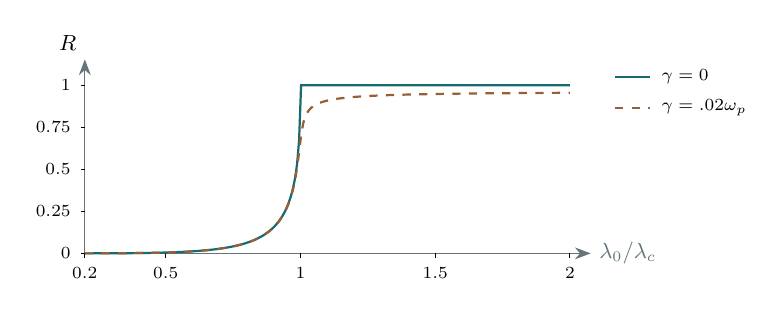
\begin{tikzpicture}[scale=.88,transform shape]
\draw[axis] (0,0.0)--(7.3,0.0) node[right] {$\lambda_0/\lambda_c$};
\draw[axis] (0,0)--(0,2.8);
\node[above left] at (0,2.8) {$R$};
\draw[thin] (0.000000,0.0)--(0.000000,-0.06);\node[below,font=\scriptsize] at (0.000000,-0.08) {$ 0.2 $};
\draw[thin] (1.166667,0.0)--(1.166667,-0.06);\node[below,font=\scriptsize] at (1.166667,-0.08) {$ 0.5 $};
\draw[thin] (3.111111,0.0)--(3.111111,-0.06);\node[below,font=\scriptsize] at (3.111111,-0.08) {$ 1 $};
\draw[thin] (5.055556,0.0)--(5.055556,-0.06);\node[below,font=\scriptsize] at (5.055556,-0.08) {$ 1.5 $};
\draw[thin] (7.000000,0.0)--(7.000000,-0.06);\node[below,font=\scriptsize] at (7.000000,-0.08) {$ 2 $};
\draw[thin] (0,0.000000)--(-.06,0.000000);\node[left,font=\scriptsize] at (-.08,0.000000) {$ 0 $};
\draw[thin] (0,0.606796)--(-.06,0.606796);\node[left,font=\scriptsize] at (-.08,0.606796) {$ 0.25 $};
\draw[thin] (0,1.213592)--(-.06,1.213592);\node[left,font=\scriptsize] at (-.08,1.213592) {$ 0.5 $};
\draw[thin] (0,1.820388)--(-.06,1.820388);\node[left,font=\scriptsize] at (-.08,1.820388) {$ 0.75 $};
\draw[thin] (0,2.427184)--(-.06,2.427184);\node[left,font=\scriptsize] at (-.08,2.427184) {$ 1 $};
\draw[thick,color=accent] plot coordinates {(0.0000000,0.0002528) (0.0291667,0.0002938) (0.0583333,0.0003398) (0.0875000,0.0003910) (0.1166667,0.0004481) (0.1458333,0.0005113) (0.1750000,0.0005812) (0.2041667,0.0006583) (0.2333333,0.0007430) (0.2625000,0.0008360) (0.2916667,0.0009378) (0.3208333,0.0010491) (0.3500000,0.0011703) (0.3791667,0.0013023) (0.4083333,0.0014457) (0.4375000,0.0016012) (0.4666667,0.0017696) (0.4958333,0.0019517) (0.5250000,0.0021483) (0.5541667,0.0023603) (0.5833333,0.0025887) (0.6125000,0.0028344) (0.6416667,0.0030984) (0.6708333,0.0033818) (0.7000000,0.0036858) (0.7291667,0.0040114) (0.7583333,0.0043599) (0.7875000,0.0047327) (0.8166667,0.0051311) (0.8458333,0.0055565) (0.8750000,0.0060104) (0.9041667,0.0064944) (0.9333333,0.0070102) (0.9625000,0.0075595) (0.9916667,0.0081442) (1.0208333,0.0087662) (1.0500000,0.0094276) (1.0791667,0.0101305) (1.1083333,0.0108771) (1.1375000,0.0116700) (1.1666667,0.0125116) (1.1958333,0.0134046) (1.2250000,0.0143518) (1.2541667,0.0153562) (1.2833333,0.0164210) (1.3125000,0.0175496) (1.3416667,0.0187454) (1.3708333,0.0200123) (1.4000000,0.0213541) (1.4291667,0.0227753) (1.4583333,0.0242802) (1.4875000,0.0258736) (1.5166667,0.0275607) (1.5458333,0.0293469) (1.5750000,0.0312378) (1.6041667,0.0332398) (1.6333333,0.0353593) (1.6625000,0.0376035) (1.6916667,0.0399798) (1.7208333,0.0424963) (1.7500000,0.0451617) (1.7791667,0.0479853) (1.8083333,0.0509769) (1.8375000,0.0541474) (1.8666667,0.0575084) (1.8958333,0.0610724) (1.9250000,0.0648528) (1.9541667,0.0688643) (1.9833333,0.0731227) (2.0125000,0.0776453) (2.0416667,0.0824507) (2.0708333,0.0875595) (2.1000000,0.0929938) (2.1291667,0.0987782) (2.1583333,0.1049393) (2.1875000,0.1115065) (2.2166667,0.1185123) (2.2458333,0.1259926) (2.2750000,0.1339868) (2.3041667,0.1425393) (2.3333333,0.1516990) (2.3625000,0.1615210) (2.3916667,0.1720670) (2.4208333,0.1834065) (2.4500000,0.1956182) (2.4791667,0.2087915) (2.5083333,0.2230286) (2.5375000,0.2384470) (2.5666667,0.2551823) (2.5958333,0.2733923) (2.6250000,0.2932618) (2.6541667,0.3150091) (2.6833333,0.3388944) (2.7125000,0.3652307) (2.7416667,0.3943992) (2.7708333,0.4268701) (2.8000000,0.4632325) (2.8291667,0.5042375) (2.8583333,0.5508632) (2.8875000,0.6044167) (2.9166667,0.6667009) (2.9458333,0.7403042) (2.9750000,0.8291454) (3.0041667,0.9396060) (3.0333333,1.0832632) (3.0625000,1.2852530) (3.0916667,1.6256308) (3.1208333,2.4271845) (3.1500000,2.4271845) (3.1791667,2.4271845) (3.2083333,2.4271845) (3.2375000,2.4271845) (3.2666667,2.4271845) (3.2958333,2.4271845) (3.3250000,2.4271845) (3.3541667,2.4271845) (3.3833333,2.4271845) (3.4125000,2.4271845) (3.4416667,2.4271845) (3.4708333,2.4271845) (3.5000000,2.4271845) (3.5291667,2.4271845) (3.5583333,2.4271845) (3.5875000,2.4271845) (3.6166667,2.4271845) (3.6458333,2.4271845) (3.6750000,2.4271845) (3.7041667,2.4271845) (3.7333333,2.4271845) (3.7625000,2.4271845) (3.7916667,2.4271845) (3.8208333,2.4271845) (3.8500000,2.4271845) (3.8791667,2.4271845) (3.9083333,2.4271845) (3.9375000,2.4271845) (3.9666667,2.4271845) (3.9958333,2.4271845) (4.0250000,2.4271845) (4.0541667,2.4271845) (4.0833333,2.4271845) (4.1125000,2.4271845) (4.1416667,2.4271845) (4.1708333,2.4271845) (4.2000000,2.4271845) (4.2291667,2.4271845) (4.2583333,2.4271845) (4.2875000,2.4271845) (4.3166667,2.4271845) (4.3458333,2.4271845) (4.3750000,2.4271845) (4.4041667,2.4271845) (4.4333333,2.4271845) (4.4625000,2.4271845) (4.4916667,2.4271845) (4.5208333,2.4271845) (4.5500000,2.4271845) (4.5791667,2.4271845) (4.6083333,2.4271845) (4.6375000,2.4271845) (4.6666667,2.4271845) (4.6958333,2.4271845) (4.7250000,2.4271845) (4.7541667,2.4271845) (4.7833333,2.4271845) (4.8125000,2.4271845) (4.8416667,2.4271845) (4.8708333,2.4271845) (4.9000000,2.4271845) (4.9291667,2.4271845) (4.9583333,2.4271845) (4.9875000,2.4271845) (5.0166667,2.4271845) (5.0458333,2.4271845) (5.0750000,2.4271845) (5.1041667,2.4271845) (5.1333333,2.4271845) (5.1625000,2.4271845) (5.1916667,2.4271845) (5.2208333,2.4271845) (5.2500000,2.4271845) (5.2791667,2.4271845) (5.3083333,2.4271845) (5.3375000,2.4271845) (5.3666667,2.4271845) (5.3958333,2.4271845) (5.4250000,2.4271845) (5.4541667,2.4271845) (5.4833333,2.4271845) (5.5125000,2.4271845) (5.5416667,2.4271845) (5.5708333,2.4271845) (5.6000000,2.4271845) (5.6291667,2.4271845) (5.6583333,2.4271845) (5.6875000,2.4271845) (5.7166667,2.4271845) (5.7458333,2.4271845) (5.7750000,2.4271845) (5.8041667,2.4271845) (5.8333333,2.4271845) (5.8625000,2.4271845) (5.8916667,2.4271845) (5.9208333,2.4271845) (5.9500000,2.4271845) (5.9791667,2.4271845) (6.0083333,2.4271845) (6.0375000,2.4271845) (6.0666667,2.4271845) (6.0958333,2.4271845) (6.1250000,2.4271845) (6.1541667,2.4271845) (6.1833333,2.4271845) (6.2125000,2.4271845) (6.2416667,2.4271845) (6.2708333,2.4271845) (6.3000000,2.4271845) (6.3291667,2.4271845) (6.3583333,2.4271845) (6.3875000,2.4271845) (6.4166667,2.4271845) (6.4458333,2.4271845) (6.4750000,2.4271845) (6.5041667,2.4271845) (6.5333333,2.4271845) (6.5625000,2.4271845) (6.5916667,2.4271845) (6.6208333,2.4271845) (6.6500000,2.4271845) (6.6791667,2.4271845) (6.7083333,2.4271845) (6.7375000,2.4271845) (6.7666667,2.4271845) (6.7958333,2.4271845) (6.8250000,2.4271845) (6.8541667,2.4271845) (6.8833333,2.4271845) (6.9125000,2.4271845) (6.9416667,2.4271845) (6.9708333,2.4271845) (7.0000000,2.4271845)};
\draw[thick,color=accent] (7.65,2.55)--(8.15,2.55);\node[right,font=\scriptsize] at (8.2,2.55) {$\gamma=0$};
\draw[thick,dashed,color=warm] plot coordinates {(0.0000000,0.0002528) (0.0291667,0.0002938) (0.0583333,0.0003398) (0.0875000,0.0003910) (0.1166667,0.0004481) (0.1458333,0.0005113) (0.1750000,0.0005812) (0.2041667,0.0006583) (0.2333333,0.0007430) (0.2625000,0.0008360) (0.2916667,0.0009378) (0.3208333,0.0010490) (0.3500000,0.0011703) (0.3791667,0.0013022) (0.4083333,0.0014456) (0.4375000,0.0016011) (0.4666667,0.0017695) (0.4958333,0.0019516) (0.5250000,0.0021482) (0.5541667,0.0023602) (0.5833333,0.0025886) (0.6125000,0.0028342) (0.6416667,0.0030982) (0.6708333,0.0033816) (0.7000000,0.0036855) (0.7291667,0.0040111) (0.7583333,0.0043596) (0.7875000,0.0047323) (0.8166667,0.0051307) (0.8458333,0.0055560) (0.8750000,0.0060099) (0.9041667,0.0064938) (0.9333333,0.0070095) (0.9625000,0.0075588) (0.9916667,0.0081434) (1.0208333,0.0087653) (1.0500000,0.0094265) (1.0791667,0.0101293) (1.1083333,0.0108758) (1.1375000,0.0116685) (1.1666667,0.0125099) (1.1958333,0.0134027) (1.2250000,0.0143497) (1.2541667,0.0153539) (1.2833333,0.0164184) (1.3125000,0.0175467) (1.3416667,0.0187422) (1.3708333,0.0200087) (1.4000000,0.0213502) (1.4291667,0.0227709) (1.4583333,0.0242753) (1.4875000,0.0258682) (1.5166667,0.0275547) (1.5458333,0.0293402) (1.5750000,0.0312304) (1.6041667,0.0332316) (1.6333333,0.0353503) (1.6625000,0.0375934) (1.6916667,0.0399687) (1.7208333,0.0424840) (1.7500000,0.0451480) (1.7791667,0.0479700) (1.8083333,0.0509601) (1.8375000,0.0541288) (1.8666667,0.0574877) (1.8958333,0.0610494) (1.9250000,0.0648272) (1.9541667,0.0688359) (1.9833333,0.0730911) (2.0125000,0.0776102) (2.0416667,0.0824116) (2.0708333,0.0875159) (2.1000000,0.0929453) (2.1291667,0.0987239) (2.1583333,0.1048786) (2.1875000,0.1114386) (2.2166667,0.1184363) (2.2458333,0.1259072) (2.2750000,0.1338908) (2.3041667,0.1424311) (2.3333333,0.1515769) (2.3625000,0.1613829) (2.3916667,0.1719103) (2.4208333,0.1832282) (2.4500000,0.1954148) (2.4791667,0.2085587) (2.5083333,0.2227612) (2.5375000,0.2381386) (2.5666667,0.2548250) (2.5958333,0.2729762) (2.6250000,0.2927745) (2.6541667,0.3144348) (2.6833333,0.3382125) (2.7125000,0.3644143) (2.7416667,0.3934124) (2.7708333,0.4256639) (2.8000000,0.4617387) (2.8291667,0.5023582) (2.8583333,0.5484537) (2.8875000,0.6012542) (2.9166667,0.6624255) (2.9458333,0.7342972) (2.9750000,0.8202541) (3.0041667,0.9254312) (3.0333333,1.0579547) (3.0625000,1.2306198) (3.0916667,1.4567139) (3.1208333,1.7021301) (3.1500000,1.8723721) (3.1791667,1.9696290) (3.2083333,2.0297048) (3.2375000,2.0706217) (3.2666667,2.1005477) (3.2958333,2.1235687) (3.3250000,2.1419429) (3.3541667,2.1570228) (3.3833333,2.1696710) (3.4125000,2.1804655) (3.4416667,2.1898098) (3.4708333,2.1979947) (3.5000000,2.2052361) (3.5291667,2.2116976) (3.5583333,2.2175058) (3.5875000,2.2227607) (3.6166667,2.2275421) (3.6458333,2.2319145) (3.6750000,2.2359311) (3.7041667,2.2396358) (3.7333333,2.2430653) (3.7625000,2.2462507) (3.7916667,2.2492184) (3.8208333,2.2519909) (3.8500000,2.2545877) (3.8791667,2.2570257) (3.9083333,2.2593196) (3.9375000,2.2614823) (3.9666667,2.2635252) (3.9958333,2.2654583) (4.0250000,2.2672905) (4.0541667,2.2690297) (4.0833333,2.2706832) (4.1125000,2.2722572) (4.1416667,2.2737576) (4.1708333,2.2751894) (4.2000000,2.2765575) (4.2291667,2.2778660) (4.2583333,2.2791189) (4.2875000,2.2803197) (4.3166667,2.2814717) (4.3458333,2.2825778) (4.3750000,2.2836408) (4.4041667,2.2846632) (4.4333333,2.2856472) (4.4625000,2.2865951) (4.4916667,2.2875088) (4.5208333,2.2883901) (4.5500000,2.2892408) (4.5791667,2.2900624) (4.6083333,2.2908564) (4.6375000,2.2916242) (4.6666667,2.2923671) (4.6958333,2.2930862) (4.7250000,2.2937828) (4.7541667,2.2944577) (4.7833333,2.2951121) (4.8125000,2.2957468) (4.8416667,2.2963628) (4.8708333,2.2969608) (4.9000000,2.2975415) (4.9291667,2.2981059) (4.9583333,2.2986544) (4.9875000,2.2991878) (5.0166667,2.2997067) (5.0458333,2.3002116) (5.0750000,2.3007031) (5.1041667,2.3011818) (5.1333333,2.3016481) (5.1625000,2.3021024) (5.1916667,2.3025453) (5.2208333,2.3029772) (5.2500000,2.3033984) (5.2791667,2.3038093) (5.3083333,2.3042103) (5.3375000,2.3046018) (5.3666667,2.3049841) (5.3958333,2.3053574) (5.4250000,2.3057222) (5.4541667,2.3060786) (5.4833333,2.3064270) (5.5125000,2.3067675) (5.5416667,2.3071006) (5.5708333,2.3074264) (5.6000000,2.3077451) (5.6291667,2.3080570) (5.6583333,2.3083622) (5.6875000,2.3086611) (5.7166667,2.3089537) (5.7458333,2.3092402) (5.7750000,2.3095209) (5.8041667,2.3097959) (5.8333333,2.3100654) (5.8625000,2.3103295) (5.8916667,2.3105884) (5.9208333,2.3108422) (5.9500000,2.3110912) (5.9791667,2.3113353) (6.0083333,2.3115748) (6.0375000,2.3118097) (6.0666667,2.3120403) (6.0958333,2.3122665) (6.1250000,2.3124886) (6.1541667,2.3127067) (6.1833333,2.3129207) (6.2125000,2.3131310) (6.2416667,2.3133374) (6.2708333,2.3135402) (6.3000000,2.3137395) (6.3291667,2.3139352) (6.3583333,2.3141276) (6.3875000,2.3143167) (6.4166667,2.3145025) (6.4458333,2.3146852) (6.4750000,2.3148648) (6.5041667,2.3150414) (6.5333333,2.3152151) (6.5625000,2.3153859) (6.5916667,2.3155540) (6.6208333,2.3157193) (6.6500000,2.3158819) (6.6791667,2.3160420) (6.7083333,2.3161995) (6.7375000,2.3163545) (6.7666667,2.3165070) (6.7958333,2.3166572) (6.8250000,2.3168051) (6.8541667,2.3169507) (6.8833333,2.3170941) (6.9125000,2.3172353) (6.9416667,2.3173743) (6.9708333,2.3175113) (7.0000000,2.3176462)};
\draw[thick,dashed,color=warm] (7.65,2.0999999999999996)--(8.15,2.0999999999999996);\node[right,font=\scriptsize] at (8.2,2.0999999999999996) {$\gamma=.02\omega_p$};
\end{tikzpicture}
\figcaption{解图光5.5C\quad 保留小阻尼后截止附近的界面反射变化}
\end{minipage}\end{center}
下面沿图中正法向写出吸收功率的位置分布。谐波的单位体积平均热功率为
\[
 \overline Q(z)=\frac12\operatorname{Re}\sigma\,|E(z)|^2
 =\frac{\omega\varepsilon_0\varepsilon''}{2}|E(z)|^2,
 \quad E(z)=tE_i e^{ik_0nz-k_0\kappa z},\quad k_0=\omega/c.
\]
平均向内能流及其导数为
\[
 S(z)=\frac{\varepsilon_0cn}{2}|tE_i|^2e^{-2k_0\kappa z},\qquad
 -\frac{\dd S}{\dd z}=\varepsilon_0\omega n\kappa|E(z)|^2
 =\overline Q(z),
\]
最后一步用$2n\kappa=\varepsilon''$。有限阻尼半无限体在远处$S\to0$，从表面到无限深积分得
\[
 \int_0^\infty\overline Q(z)\,\dd z=S(0),\qquad
 \frac{S(0)}{S_i}=n|t|^2=\frac{4n}{|1+\widetilde n|^2}=1-R.
\]
因此该半无限有耗模型的吸收率为$1-R$。定义强度衰减长度$\delta_I=(2k_0\kappa)^{-1}$，从表面到深度$z$的累计吸收份额为$A(0,z)=(1-R)(1-e^{-z/\delta_I})$。解图光5.5D取$\widetilde\varepsilon=-3+.1i$，把剩余能流与已经沉积的热量画在同一深度轴上，二者之和等于进入界面的功率。无损传播支的$T$则随深度保持；无损倏逝支的净法向流为零，三种功率分配由同一场与电流关系给出。有限厚金属片还有第二界面及返回的相干场，其反射、透射由两面共同计算。
\begin{center}\begin{minipage}{.98\linewidth}\centering
\begin{tikzpicture}[scale=.88,transform shape]
\draw[axis] (0,0.0)--(7.3,0.0) node[right] {$z/\delta_I$};
\draw[axis] (0,0)--(0,2.8);
\node[above left] at (0,2.8) {$\text{入射功率份额}$};
\draw[thin] (0.000000,0.0)--(0.000000,-0.06);\node[below,font=\scriptsize] at (0.000000,-0.08) {$ 0 $};
\draw[thin] (1.400000,0.0)--(1.400000,-0.06);\node[below,font=\scriptsize] at (1.400000,-0.08) {$ 1 $};
\draw[thin] (4.200000,0.0)--(4.200000,-0.06);\node[below,font=\scriptsize] at (4.200000,-0.08) {$ 3 $};
\draw[thin] (7.000000,0.0)--(7.000000,-0.06);\node[below,font=\scriptsize] at (7.000000,-0.08) {$ 5 $};
\draw[thin] (0,0.000000)--(-.06,0.000000);\node[left,font=\scriptsize] at (-.08,0.000000) {$ 0 $};
\draw[thin] (0,0.833333)--(-.06,0.833333);\node[left,font=\scriptsize] at (-.08,0.833333) {$ 0.01 $};
\draw[thin] (0,1.666667)--(-.06,1.666667);\node[left,font=\scriptsize] at (-.08,1.666667) {$ 0.02 $};
\draw[thin] (0,2.370100)--(-.06,2.370100);\node[left,font=\scriptsize] at (-.08,2.370100) {$ 0.0284412 $};
\draw[thick,color=accent] plot coordinates {(0.0000000,2.3701002) (0.0291667,2.3212339) (0.0583333,2.2733751) (0.0875000,2.2265031) (0.1166667,2.1805975) (0.1458333,2.1356383) (0.1750000,2.0916061) (0.2041667,2.0484817) (0.2333333,2.0062465) (0.2625000,1.9648821) (0.2916667,1.9243705) (0.3208333,1.8846942) (0.3500000,1.8458359) (0.3791667,1.8077788) (0.4083333,1.7705063) (0.4375000,1.7340023) (0.4666667,1.6982510) (0.4958333,1.6632368) (0.5250000,1.6289445) (0.5541667,1.5953592) (0.5833333,1.5624664) (0.6125000,1.5302517) (0.6416667,1.4987013) (0.6708333,1.4678013) (0.7000000,1.4375384) (0.7291667,1.4078995) (0.7583333,1.3788717) (0.7875000,1.3504424) (0.8166667,1.3225992) (0.8458333,1.2953301) (0.8750000,1.2686232) (0.9041667,1.2424670) (0.9333333,1.2168500) (0.9625000,1.1917612) (0.9916667,1.1671897) (1.0208333,1.1431248) (1.0500000,1.1195561) (1.0791667,1.0964733) (1.1083333,1.0738664) (1.1375000,1.0517256) (1.1666667,1.0300413) (1.1958333,1.0088041) (1.2250000,0.9880048) (1.2541667,0.9676343) (1.2833333,0.9476837) (1.3125000,0.9281446) (1.3416667,0.9090083) (1.3708333,0.8902665) (1.4000000,0.8719111) (1.4291667,0.8539342) (1.4583333,0.8363280) (1.4875000,0.8190847) (1.5166667,0.8021970) (1.5458333,0.7856574) (1.5750000,0.7694589) (1.6041667,0.7535943) (1.6333333,0.7380568) (1.6625000,0.7228397) (1.6916667,0.7079363) (1.7208333,0.6933402) (1.7500000,0.6790451) (1.7791667,0.6650446) (1.8083333,0.6513329) (1.8375000,0.6379038) (1.8666667,0.6247516) (1.8958333,0.6118706) (1.9250000,0.5992552) (1.9541667,0.5868998) (1.9833333,0.5747992) (2.0125000,0.5629481) (2.0416667,0.5513414) (2.0708333,0.5399739) (2.1000000,0.5288408) (2.1291667,0.5179373) (2.1583333,0.5072586) (2.1875000,0.4968000) (2.2166667,0.4865571) (2.2458333,0.4765253) (2.2750000,0.4667004) (2.3041667,0.4570781) (2.3333333,0.4476541) (2.3625000,0.4384245) (2.3916667,0.4293851) (2.4208333,0.4205321) (2.4500000,0.4118617) (2.4791667,0.4033700) (2.5083333,0.3950534) (2.5375000,0.3869082) (2.5666667,0.3789310) (2.5958333,0.3711183) (2.6250000,0.3634666) (2.6541667,0.3559727) (2.6833333,0.3486334) (2.7125000,0.3414453) (2.7416667,0.3344054) (2.7708333,0.3275107) (2.8000000,0.3207582) (2.8291667,0.3141448) (2.8583333,0.3076679) (2.8875000,0.3013244) (2.9166667,0.2951118) (2.9458333,0.2890272) (2.9750000,0.2830681) (3.0041667,0.2772319) (3.0333333,0.2715159) (3.0625000,0.2659179) (3.0916667,0.2604352) (3.1208333,0.2550656) (3.1500000,0.2498067) (3.1791667,0.2446563) (3.2083333,0.2396120) (3.2375000,0.2346717) (3.2666667,0.2298333) (3.2958333,0.2250946) (3.3250000,0.2204537) (3.3541667,0.2159084) (3.3833333,0.2114568) (3.4125000,0.2070970) (3.4416667,0.2028272) (3.4708333,0.1986453) (3.5000000,0.1945497) (3.5291667,0.1905385) (3.5583333,0.1866100) (3.5875000,0.1827625) (3.6166667,0.1789943) (3.6458333,0.1753039) (3.6750000,0.1716895) (3.7041667,0.1681496) (3.7333333,0.1646827) (3.7625000,0.1612873) (3.7916667,0.1579619) (3.8208333,0.1547051) (3.8500000,0.1515154) (3.8791667,0.1483915) (3.9083333,0.1453320) (3.9375000,0.1423356) (3.9666667,0.1394009) (3.9958333,0.1365268) (4.0250000,0.1337119) (4.0541667,0.1309551) (4.0833333,0.1282550) (4.1125000,0.1256107) (4.1416667,0.1230209) (4.1708333,0.1204845) (4.2000000,0.1180003) (4.2291667,0.1155674) (4.2583333,0.1131847) (4.2875000,0.1108511) (4.3166667,0.1085656) (4.3458333,0.1063272) (4.3750000,0.1041349) (4.4041667,0.1019879) (4.4333333,0.0998851) (4.4625000,0.0978257) (4.4916667,0.0958088) (4.5208333,0.0938334) (4.5500000,0.0918988) (4.5791667,0.0900040) (4.6083333,0.0881483) (4.6375000,0.0863309) (4.6666667,0.0845509) (4.6958333,0.0828077) (4.7250000,0.0811004) (4.7541667,0.0794283) (4.7833333,0.0777906) (4.8125000,0.0761867) (4.8416667,0.0746159) (4.8708333,0.0730775) (4.9000000,0.0715708) (4.9291667,0.0700952) (4.9583333,0.0686500) (4.9875000,0.0672346) (5.0166667,0.0658483) (5.0458333,0.0644907) (5.0750000,0.0631610) (5.1041667,0.0618588) (5.1333333,0.0605834) (5.1625000,0.0593343) (5.1916667,0.0581110) (5.2208333,0.0569128) (5.2500000,0.0557394) (5.2791667,0.0545902) (5.3083333,0.0534647) (5.3375000,0.0523623) (5.3666667,0.0512827) (5.3958333,0.0502254) (5.4250000,0.0491899) (5.4541667,0.0481757) (5.4833333,0.0471824) (5.5125000,0.0462096) (5.5416667,0.0452569) (5.5708333,0.0443238) (5.6000000,0.0434099) (5.6291667,0.0425149) (5.6583333,0.0416383) (5.6875000,0.0407798) (5.7166667,0.0399390) (5.7458333,0.0391156) (5.7750000,0.0383091) (5.8041667,0.0375193) (5.8333333,0.0367457) (5.8625000,0.0359881) (5.8916667,0.0352461) (5.9208333,0.0345194) (5.9500000,0.0338077) (5.9791667,0.0331106) (6.0083333,0.0324280) (6.0375000,0.0317594) (6.0666667,0.0311046) (6.0958333,0.0304632) (6.1250000,0.0298352) (6.1541667,0.0292200) (6.1833333,0.0286176) (6.2125000,0.0280275) (6.2416667,0.0274497) (6.2708333,0.0268837) (6.3000000,0.0263294) (6.3291667,0.0257866) (6.3583333,0.0252549) (6.3875000,0.0247342) (6.4166667,0.0242242) (6.4458333,0.0237248) (6.4750000,0.0232356) (6.5041667,0.0227566) (6.5333333,0.0222874) (6.5625000,0.0218279) (6.5916667,0.0213778) (6.6208333,0.0209371) (6.6500000,0.0205054) (6.6791667,0.0200826) (6.7083333,0.0196685) (6.7375000,0.0192630) (6.7666667,0.0188659) (6.7958333,0.0184769) (6.8250000,0.0180959) (6.8541667,0.0177228) (6.8833333,0.0173574) (6.9125000,0.0169996) (6.9416667,0.0166491) (6.9708333,0.0163058) (7.0000000,0.0159696)};
\draw[thick,color=accent] (7.65,2.55)--(8.15,2.55);\node[right,font=\scriptsize] at (8.2,2.55) {$S(z)/S_i$};
\draw[thick,dashed,color=warm] plot coordinates {(0.0000000,0.0000000) (0.0291667,0.0488663) (0.0583333,0.0967251) (0.0875000,0.1435971) (0.1166667,0.1895027) (0.1458333,0.2344619) (0.1750000,0.2784941) (0.2041667,0.3216185) (0.2333333,0.3638537) (0.2625000,0.4052181) (0.2916667,0.4457297) (0.3208333,0.4854060) (0.3500000,0.5242643) (0.3791667,0.5623214) (0.4083333,0.5995939) (0.4375000,0.6360979) (0.4666667,0.6718492) (0.4958333,0.7068634) (0.5250000,0.7411557) (0.5541667,0.7747410) (0.5833333,0.8076339) (0.6125000,0.8398485) (0.6416667,0.8713990) (0.6708333,0.9022989) (0.7000000,0.9325618) (0.7291667,0.9622007) (0.7583333,0.9912285) (0.7875000,1.0196578) (0.8166667,1.0475010) (0.8458333,1.0747701) (0.8750000,1.1014770) (0.9041667,1.1276332) (0.9333333,1.1532502) (0.9625000,1.1783390) (0.9916667,1.2029105) (1.0208333,1.2269754) (1.0500000,1.2505441) (1.0791667,1.2736269) (1.1083333,1.2962338) (1.1375000,1.3183746) (1.1666667,1.3400589) (1.1958333,1.3612961) (1.2250000,1.3820954) (1.2541667,1.4024659) (1.2833333,1.4224165) (1.3125000,1.4419556) (1.3416667,1.4610919) (1.3708333,1.4798337) (1.4000000,1.4981891) (1.4291667,1.5161660) (1.4583333,1.5337722) (1.4875000,1.5510155) (1.5166667,1.5679032) (1.5458333,1.5844428) (1.5750000,1.6006413) (1.6041667,1.6165059) (1.6333333,1.6320434) (1.6625000,1.6472605) (1.6916667,1.6621639) (1.7208333,1.6767600) (1.7500000,1.6910551) (1.7791667,1.7050556) (1.8083333,1.7187673) (1.8375000,1.7321964) (1.8666667,1.7453486) (1.8958333,1.7582296) (1.9250000,1.7708450) (1.9541667,1.7832004) (1.9833333,1.7953010) (2.0125000,1.8071521) (2.0416667,1.8187588) (2.0708333,1.8301263) (2.1000000,1.8412594) (2.1291667,1.8521629) (2.1583333,1.8628416) (2.1875000,1.8733002) (2.2166667,1.8835431) (2.2458333,1.8935749) (2.2750000,1.9033998) (2.3041667,1.9130221) (2.3333333,1.9224461) (2.3625000,1.9316757) (2.3916667,1.9407151) (2.4208333,1.9495681) (2.4500000,1.9582385) (2.4791667,1.9667302) (2.5083333,1.9750468) (2.5375000,1.9831920) (2.5666667,1.9911692) (2.5958333,1.9989819) (2.6250000,2.0066336) (2.6541667,2.0141275) (2.6833333,2.0214668) (2.7125000,2.0286549) (2.7416667,2.0356948) (2.7708333,2.0425895) (2.8000000,2.0493420) (2.8291667,2.0559554) (2.8583333,2.0624323) (2.8875000,2.0687758) (2.9166667,2.0749884) (2.9458333,2.0810730) (2.9750000,2.0870321) (3.0041667,2.0928683) (3.0333333,2.0985843) (3.0625000,2.1041823) (3.0916667,2.1096650) (3.1208333,2.1150346) (3.1500000,2.1202935) (3.1791667,2.1254439) (3.2083333,2.1304882) (3.2375000,2.1354285) (3.2666667,2.1402669) (3.2958333,2.1450056) (3.3250000,2.1496465) (3.3541667,2.1541918) (3.3833333,2.1586434) (3.4125000,2.1630032) (3.4416667,2.1672730) (3.4708333,2.1714549) (3.5000000,2.1755505) (3.5291667,2.1795617) (3.5583333,2.1834902) (3.5875000,2.1873377) (3.6166667,2.1911059) (3.6458333,2.1947963) (3.6750000,2.1984107) (3.7041667,2.2019506) (3.7333333,2.2054175) (3.7625000,2.2088129) (3.7916667,2.2121383) (3.8208333,2.2153951) (3.8500000,2.2185848) (3.8791667,2.2217087) (3.9083333,2.2247682) (3.9375000,2.2277646) (3.9666667,2.2306993) (3.9958333,2.2335734) (4.0250000,2.2363883) (4.0541667,2.2391451) (4.0833333,2.2418452) (4.1125000,2.2444895) (4.1416667,2.2470793) (4.1708333,2.2496157) (4.2000000,2.2520999) (4.2291667,2.2545328) (4.2583333,2.2569155) (4.2875000,2.2592491) (4.3166667,2.2615346) (4.3458333,2.2637730) (4.3750000,2.2659653) (4.4041667,2.2681123) (4.4333333,2.2702151) (4.4625000,2.2722745) (4.4916667,2.2742914) (4.5208333,2.2762668) (4.5500000,2.2782014) (4.5791667,2.2800962) (4.6083333,2.2819519) (4.6375000,2.2837693) (4.6666667,2.2855493) (4.6958333,2.2872925) (4.7250000,2.2889998) (4.7541667,2.2906719) (4.7833333,2.2923096) (4.8125000,2.2939135) (4.8416667,2.2954843) (4.8708333,2.2970227) (4.9000000,2.2985294) (4.9291667,2.3000050) (4.9583333,2.3014502) (4.9875000,2.3028656) (5.0166667,2.3042519) (5.0458333,2.3056095) (5.0750000,2.3069392) (5.1041667,2.3082414) (5.1333333,2.3095168) (5.1625000,2.3107659) (5.1916667,2.3119892) (5.2208333,2.3131874) (5.2500000,2.3143608) (5.2791667,2.3155100) (5.3083333,2.3166355) (5.3375000,2.3177379) (5.3666667,2.3188175) (5.3958333,2.3198748) (5.4250000,2.3209103) (5.4541667,2.3219245) (5.4833333,2.3229178) (5.5125000,2.3238906) (5.5416667,2.3248433) (5.5708333,2.3257764) (5.6000000,2.3266903) (5.6291667,2.3275853) (5.6583333,2.3284619) (5.6875000,2.3293204) (5.7166667,2.3301612) (5.7458333,2.3309846) (5.7750000,2.3317911) (5.8041667,2.3325809) (5.8333333,2.3333545) (5.8625000,2.3341121) (5.8916667,2.3348541) (5.9208333,2.3355808) (5.9500000,2.3362925) (5.9791667,2.3369896) (6.0083333,2.3376722) (6.0375000,2.3383408) (6.0666667,2.3389956) (6.0958333,2.3396370) (6.1250000,2.3402650) (6.1541667,2.3408802) (6.1833333,2.3414826) (6.2125000,2.3420727) (6.2416667,2.3426505) (6.2708333,2.3432165) (6.3000000,2.3437708) (6.3291667,2.3443136) (6.3583333,2.3448453) (6.3875000,2.3453660) (6.4166667,2.3458760) (6.4458333,2.3463754) (6.4750000,2.3468646) (6.5041667,2.3473436) (6.5333333,2.3478128) (6.5625000,2.3482723) (6.5916667,2.3487224) (6.6208333,2.3491631) (6.6500000,2.3495948) (6.6791667,2.3500176) (6.7083333,2.3504317) (6.7375000,2.3508372) (6.7666667,2.3512343) (6.7958333,2.3516233) (6.8250000,2.3520043) (6.8541667,2.3523774) (6.8833333,2.3527428) (6.9125000,2.3531006) (6.9416667,2.3534511) (6.9708333,2.3537944) (7.0000000,2.3541306)};
\draw[thick,dashed,color=warm] (7.65,2.0999999999999996)--(8.15,2.0999999999999996);\node[right,font=\scriptsize] at (8.2,2.0999999999999996) {$A(0,z)$};
\end{tikzpicture}
\figcaption{解图光5.5D\quad $\widetilde\varepsilon=-3+0.1i$时进入功率逐层沉积为热}
\end{minipage}\end{center}


\Needspace{13\baselineskip}

\pdfbookmark[2]{第 6 题 电离层的反射与布儒斯特角}{q6}

\section*{第 6 题\quad 电离层的反射与布儒斯特角}\label{q:6}

将电离层看作均匀、无碰撞、无外磁场的冷等离子体，电子数密度为$N$，重离子响应忽略。它与非电离大气之间有平面突变界面，大气折射率取1。（1）当$\nu=2\nu_p$或$\nu\ll\nu_p$时，求从大气正入射的能量反射率，其中$\nu_p$为等离子体频率。（2）在允许传播的情形，若反射光只含垂直于入射面的振动，入射角应是多少？明确给出$\nu=2\nu_p$的结果。

\begin{center}\begin{minipage}{.98\linewidth}\centering
\begin{tikzpicture}[scale=.9,transform shape]
\draw[object] (-3.00000,0.00000)--(3.00000,0.00000);\node[left] at (-0.70000,1.40000) {大气 $n_1=1$};\node[below] at (0.00000,-2.80000) {等离子体 $\varepsilon=1-\nu_p^2/\nu^2$};\draw[motion] (-0.20000,2.00000)--(-0.20000,0.00000);
\draw[motion] (-0.20000,0.00000)--(-0.20000,-2.00000);\draw[force] (0.20000,0.00000)--(0.20000,2.00000);\node[right] at (0.80000,1.00000) {反射 $R$};
\end{tikzpicture}
\figcaption{图光5.6\quad 正入射能量分配先按频率区间判断。}
\end{minipage}\end{center}

\Needspace{6\baselineskip}\subsection*{解答}


图光5.6取上方为折射率1的大气，下方为均匀冷等离子体，界面为平面突变；重离子近似固定，忽略碰撞与外磁场。电子数密度为$N$。一维电子位移给出集体频率尺度，横波受迫极化使用同一电子数密度。

如解图光5.6B，考察一段平面电子层相对固定正离子沿一维位移$\xi$。两端露出的正、负面电荷产生回复场，层内极化为$P=-Ne\xi$。在该集体纵向位移中，回复场为$E=-P/\varepsilon_0=Ne\xi/\varepsilon_0$，每电子受力$-eE$，所以
\[
 m_e\ddot\xi=-\frac{Ne^2}{\varepsilon_0}\xi.
\]
外来频率$\omega$的横场则驱动自由电子$m_e\ddot x=-eE$，位移$x=eE/(m_e\omega^2)$，极化$P=-Nex$。由这两个方程得到同一频率尺度和横波介电常数
\[
\omega_p^2=\frac{Ne^2}{\varepsilon_0m_e},\qquad
\nu_p=\frac{\omega_p}{2\pi},\qquad
\varepsilon=1-\frac{\omega_p^2}{\omega^2}=1-\frac{\nu_p^2}{\nu^2}.
\]
正离子质量较大，受迫响应中的倒数质量权重较小，在当前模型中略去。角频率与普通频率满足$\omega=2\pi\nu$，其比值在介电式中相同。
\begin{center}\begin{minipage}{.98\linewidth}\centering
\begin{tikzpicture}[scale=.95,transform shape]
\node[color=accent] at (0,.6) {$+$};\node[color=warm] at (0.5,-.3) {$-$};
\node[color=accent] at (1,.6) {$+$};\node[color=warm] at (1.5,-.3) {$-$};
\node[color=accent] at (2,.6) {$+$};\node[color=warm] at (2.5,-.3) {$-$};
\node[color=accent] at (3,.6) {$+$};\node[color=warm] at (3.5,-.3) {$-$};
\node[color=accent] at (4,.6) {$+$};\node[color=warm] at (4.5,-.3) {$-$};
\draw[guide] (0,-.7)--(0,1);\draw[guide] (4,-.7)--(4,1);
\draw[force] (.7,1.5)--(3.2,1.5) node[midway,above] {$E=Ne\xi/\varepsilon_0$};
\draw[motion] (3.2,-1)--(1.8,-1) node[midway,below] {$-eE$};
\draw[<->] (0,-1.6)--(.5,-1.6) node[midway,below] {$\xi$};
\node[right] at (4.8,.6) {固定离子};\node[right] at (4.8,-.3) {电子位移};
\end{tikzpicture}
\figcaption{解图光5.6B\quad 电子集体位移产生与位移反向的电子回复力}
\end{minipage}\end{center}
在$\nu=2\nu_p$时，$\varepsilon=3/4$、$n=\sqrt3/2=.8660254$为正实数。取向内传播的透射波，正入射切向场连续为$1+r=t$、$1-r=nt$，故$r=(1-n)/(1+n)$、$t=2/(1+n)$，功率反射率为
\[
\boxed{R=\left(\frac{1-n}{1+n}\right)^2
=\left(\frac{2-\sqrt3}{2+\sqrt3}\right)^2
=5.1548\times10^{-3}}.
\]
透射功率比为$T=n|t|^2=1-R=.9948452$，约$0.515\%$功率反射，其余在该无损模型内向下传播。解图光5.6C在同一频率轴上画出法向反射率，$\nu/\nu_p=2$位于低反射的传播区。

当$0<\nu<\nu_p$时，$\varepsilon<0$，取$\widetilde n=i\kappa$、$\kappa=\sqrt{\nu_p^2/\nu^2-1}>0$，透射场沿进入等离子体的正法向衰减。代入同一界面关系有
\[
r=\frac{1-i\kappa}{1+i\kappa},\quad
\boxed{R=|r|^2=1}.
\]
这一结果在整个低于截止的无损半无限区间严格成立，包含$\nu\ll\nu_p$。电、磁场的相对相位使平均法向透射流为零，碰撞被略去也使体热功率为零。
\begin{center}\begin{minipage}{.98\linewidth}\centering
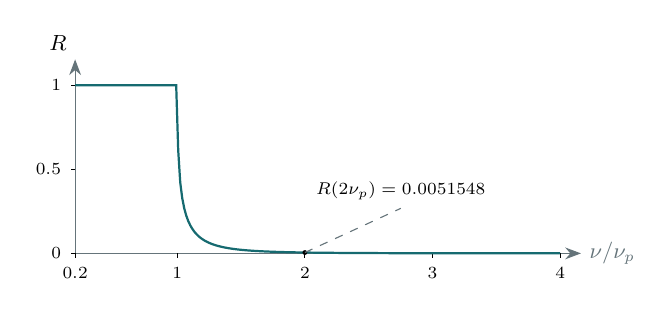
\begin{tikzpicture}[scale=.88,transform shape]
\draw[axis] (0,0.0)--(7.3,0.0) node[right] {$\nu/\nu_p$};
\draw[axis] (0,0)--(0,2.8);
\node[above left] at (0,2.8) {$R$};
\draw[thin] (0.000000,0.0)--(0.000000,-0.06);\node[below,font=\scriptsize] at (0.000000,-0.08) {$ 0.2 $};
\draw[thin] (1.473684,0.0)--(1.473684,-0.06);\node[below,font=\scriptsize] at (1.473684,-0.08) {$ 1 $};
\draw[thin] (3.315789,0.0)--(3.315789,-0.06);\node[below,font=\scriptsize] at (3.315789,-0.08) {$ 2 $};
\draw[thin] (5.157895,0.0)--(5.157895,-0.06);\node[below,font=\scriptsize] at (5.157895,-0.08) {$ 3 $};
\draw[thin] (7.000000,0.0)--(7.000000,-0.06);\node[below,font=\scriptsize] at (7.000000,-0.08) {$ 4 $};
\draw[thin] (0,0.000000)--(-.06,0.000000);\node[left,font=\scriptsize] at (-.08,0.000000) {$ 0 $};

\draw[thin] (0,1.213592)--(-.06,1.213592);\node[left,font=\scriptsize] at (-.08,1.213592) {$ 0.5 $};
\draw[thin] (0,2.427184)--(-.06,2.427184);\node[left,font=\scriptsize] at (-.08,2.427184) {$ 1 $};
\draw[thick,color=accent] plot coordinates {(0.0000000,2.4271845) (0.0291667,2.4271845) (0.0583333,2.4271845) (0.0875000,2.4271845) (0.1166667,2.4271845) (0.1458333,2.4271845) (0.1750000,2.4271845) (0.2041667,2.4271845) (0.2333333,2.4271845) (0.2625000,2.4271845) (0.2916667,2.4271845) (0.3208333,2.4271845) (0.3500000,2.4271845) (0.3791667,2.4271845) (0.4083333,2.4271845) (0.4375000,2.4271845) (0.4666667,2.4271845) (0.4958333,2.4271845) (0.5250000,2.4271845) (0.5541667,2.4271845) (0.5833333,2.4271845) (0.6125000,2.4271845) (0.6416667,2.4271845) (0.6708333,2.4271845) (0.7000000,2.4271845) (0.7291667,2.4271845) (0.7583333,2.4271845) (0.7875000,2.4271845) (0.8166667,2.4271845) (0.8458333,2.4271845) (0.8750000,2.4271845) (0.9041667,2.4271845) (0.9333333,2.4271845) (0.9625000,2.4271845) (0.9916667,2.4271845) (1.0208333,2.4271845) (1.0500000,2.4271845) (1.0791667,2.4271845) (1.1083333,2.4271845) (1.1375000,2.4271845) (1.1666667,2.4271845) (1.1958333,2.4271845) (1.2250000,2.4271845) (1.2541667,2.4271845) (1.2833333,2.4271845) (1.3125000,2.4271845) (1.3416667,2.4271845) (1.3708333,2.4271845) (1.4000000,2.4271845) (1.4291667,2.4271845) (1.4583333,2.4271845) (1.4875000,1.4875637) (1.5166667,1.0246024) (1.5458333,0.7951937) (1.5750000,0.6479696) (1.6041667,0.5433154) (1.6333333,0.4644961) (1.6625000,0.4028376) (1.6916667,0.3532750) (1.7208333,0.3126065) (1.7500000,0.2786895) (1.7791667,0.2500271) (1.8083333,0.2255376) (1.8375000,0.2044175) (1.8666667,0.1860565) (1.8958333,0.1699819) (1.9250000,0.1558221) (1.9541667,0.1432802) (1.9833333,0.1321165) (2.0125000,0.1221353) (2.0416667,0.1131753) (2.0708333,0.1051021) (2.1000000,0.0978034) (2.1291667,0.0911841) (2.1583333,0.0851637) (2.1875000,0.0796731) (2.2166667,0.0746532) (2.2458333,0.0700528) (2.2750000,0.0658277) (2.3041667,0.0619391) (2.3333333,0.0583533) (2.3625000,0.0550406) (2.3916667,0.0519749) (2.4208333,0.0491331) (2.4500000,0.0464947) (2.4791667,0.0440415) (2.5083333,0.0417572) (2.5375000,0.0396274) (2.5666667,0.0376389) (2.5958333,0.0357802) (2.6250000,0.0340407) (2.6541667,0.0324109) (2.6833333,0.0308822) (2.7125000,0.0294468) (2.7416667,0.0280977) (2.7708333,0.0268284) (2.8000000,0.0256332) (2.8291667,0.0245066) (2.8583333,0.0234438) (2.8875000,0.0224404) (2.9166667,0.0214922) (2.9458333,0.0205955) (2.9750000,0.0197469) (3.0041667,0.0189431) (3.0333333,0.0181813) (3.0625000,0.0174588) (3.0916667,0.0167731) (3.1208333,0.0161219) (3.1500000,0.0155030) (3.1791667,0.0149145) (3.2083333,0.0143546) (3.2375000,0.0138215) (3.2666667,0.0133137) (3.2958333,0.0128297) (3.3250000,0.0123682) (3.3541667,0.0119278) (3.3833333,0.0115074) (3.4125000,0.0111059) (3.4416667,0.0107223) (3.4708333,0.0103555) (3.5000000,0.0100047) (3.5291667,0.0096689) (3.5583333,0.0093476) (3.5875000,0.0090398) (3.6166667,0.0087448) (3.6458333,0.0084621) (3.6750000,0.0081910) (3.7041667,0.0079310) (3.7333333,0.0076814) (3.7625000,0.0074417) (3.7916667,0.0072116) (3.8208333,0.0069905) (3.8500000,0.0067779) (3.8791667,0.0065736) (3.9083333,0.0063771) (3.9375000,0.0061880) (3.9666667,0.0060060) (3.9958333,0.0058307) (4.0250000,0.0056620) (4.0541667,0.0054994) (4.0833333,0.0053428) (4.1125000,0.0051917) (4.1416667,0.0050461) (4.1708333,0.0049056) (4.2000000,0.0047701) (4.2291667,0.0046393) (4.2583333,0.0045131) (4.2875000,0.0043912) (4.3166667,0.0042734) (4.3458333,0.0041596) (4.3750000,0.0040497) (4.4041667,0.0039434) (4.4333333,0.0038406) (4.4625000,0.0037413) (4.4916667,0.0036451) (4.5208333,0.0035521) (4.5500000,0.0034621) (4.5791667,0.0033749) (4.6083333,0.0032906) (4.6375000,0.0032088) (4.6666667,0.0031297) (4.6958333,0.0030530) (4.7250000,0.0029786) (4.7541667,0.0029066) (4.7833333,0.0028367) (4.8125000,0.0027690) (4.8416667,0.0027033) (4.8708333,0.0026395) (4.9000000,0.0025777) (4.9291667,0.0025176) (4.9583333,0.0024594) (4.9875000,0.0024028) (5.0166667,0.0023479) (5.0458333,0.0022945) (5.0750000,0.0022427) (5.1041667,0.0021923) (5.1333333,0.0021434) (5.1625000,0.0020959) (5.1916667,0.0020496) (5.2208333,0.0020047) (5.2500000,0.0019610) (5.2791667,0.0019185) (5.3083333,0.0018771) (5.3375000,0.0018369) (5.3666667,0.0017977) (5.3958333,0.0017596) (5.4250000,0.0017226) (5.4541667,0.0016865) (5.4833333,0.0016513) (5.5125000,0.0016171) (5.5416667,0.0015837) (5.5708333,0.0015513) (5.6000000,0.0015196) (5.6291667,0.0014888) (5.6583333,0.0014587) (5.6875000,0.0014295) (5.7166667,0.0014009) (5.7458333,0.0013731) (5.7750000,0.0013460) (5.8041667,0.0013195) (5.8333333,0.0012937) (5.8625000,0.0012685) (5.8916667,0.0012440) (5.9208333,0.0012200) (5.9500000,0.0011966) (5.9791667,0.0011738) (6.0083333,0.0011515) (6.0375000,0.0011298) (6.0666667,0.0011086) (6.0958333,0.0010878) (6.1250000,0.0010676) (6.1541667,0.0010478) (6.1833333,0.0010285) (6.2125000,0.0010096) (6.2416667,0.0009912) (6.2708333,0.0009732) (6.3000000,0.0009556) (6.3291667,0.0009384) (6.3583333,0.0009216) (6.3875000,0.0009052) (6.4166667,0.0008891) (6.4458333,0.0008734) (6.4750000,0.0008580) (6.5041667,0.0008430) (6.5333333,0.0008283) (6.5625000,0.0008140) (6.5916667,0.0007999) (6.6208333,0.0007861) (6.6500000,0.0007727) (6.6791667,0.0007595) (6.7083333,0.0007466) (6.7375000,0.0007340) (6.7666667,0.0007217) (6.7958333,0.0007096) (6.8250000,0.0006978) (6.8541667,0.0006862) (6.8833333,0.0006748) (6.9125000,0.0006637) (6.9416667,0.0006528) (6.9708333,0.0006422) (7.0000000,0.0006318)};
\fill (3.315789,.012512) circle(.035);\draw[guide] (3.315789,.012512)--(4.7,.65);\node[above,font=\scriptsize] at (4.7,.65) {$R(2\nu_p)=0.0051548$};
\end{tikzpicture}
\figcaption{解图光5.6C\quad 无碰撞突变界面的法向反射率}
\end{minipage}\end{center}
再求斜入射时的偏振。设实传播支$\nu>\nu_p$，角度从法线量起。记$k_0=\omega/c$、$q_z=k_z/k_0$，切向波矢连续给$q_z^2=n^2-\sin^2\theta_i$。以下$s$电场沿同一垂直图面方向，$p$基矢按$\boldsymbol s\times\hat{\boldsymbol k}$取向，两个反射振幅为
\[
 r_s=\frac{\cos\theta_i-q_z}{\cos\theta_i+q_z},\qquad
 r_p=\frac{n^2\cos\theta_i-q_z}{n^2\cos\theta_i+q_z}.
\]
反射仅保留$s$需要$r_p=0$且输入本来含非零$s$分量。取$q_z=n\cos\theta_t$，$r_p=0$给$n\cos\theta_i=\cos\theta_t$；与Snell关系一起得到
\[
\theta_i+\theta_t=\frac\pi2,\quad
\sin\theta_i=n\sin\theta_t=n\cos\theta_i,
\]
故布儒斯特角为
\[
\boxed{\theta_B=\arctan n
=\arctan\sqrt{1-\nu_p^2/\nu^2}}.
\]
在$\nu=2\nu_p$时，数值为
\[
\boxed{\theta_B=40.8934^\circ\simeq40^\circ54'}.
\]
解图光5.6A按这个角度画出两条实际反射、折射方向，它们相互垂直；$s$方向垂直图面，$p$方向在图面内。空气射向较小实折射率还有临界角$\theta_c=\arcsin n=60^\circ$。因为$\sin\theta_B=n/\sqrt{1+n^2}<n$，所以$\theta_B<\theta_c$，布儒斯特工作点属于可传播区。
\begin{center}\begin{minipage}{.98\linewidth}\centering
\begin{tikzpicture}[scale=.9,transform shape]
\draw[object] (-3.2,0)--(3.7,0);\draw[guide] (0,-2.5)--(0,2.6);
\draw[motion] (-1.7020995,1.9654153)--(0,0);\draw[motion] (0,0)--(1.7020995,1.9654153);\draw[force] (0,0)--(1.9654153,-1.7020995);
\draw[thin] (0.2618615,0.3023716)--(0.5642330,0.0405101)--(0.3023716,-0.2618615);
\node[above left] at (-1.8,2) {入射};\node[above right] at (1.8,2) {反射$s$};\node[right] at (2.1,-1.65) {折射};
\node[left] at (-.4,.8) {$\theta_B$};\node[right] at (.35,-.75) {$\theta_t$};\node[left] at (-2,.6) {$n_1=1$};\node[left] at (-1.3,-1.9) {$n=\sqrt3/2$};
\node[above] at (0,2.7) {$\theta_B+\theta_t=90^\circ$};
\end{tikzpicture}
\figcaption{解图光5.6A\quad 两倍等离子体频率的布儒斯特几何与正交反射折射线}
\end{minipage}\end{center}
解图光5.6D同时画$s,p$功率反射率：在$40.8934^\circ$处$p$分量为零，$s$分量仍有反射；大于60度后两者均为全反射。若输入只有$p$，该布儒斯特设置的反射功率为零；对含$s$的输入，留下的反射束沿$s$。
\begin{center}\begin{minipage}{.98\linewidth}\centering
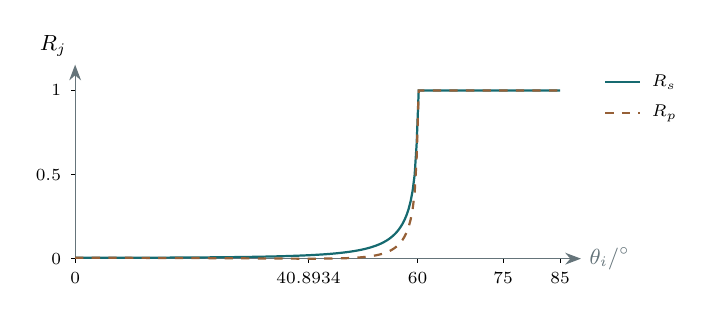
\begin{tikzpicture}[scale=.88,transform shape]
\draw[axis] (0,0.0)--(7.3,0.0) node[right] {$\theta_i/{}^\circ$};
\draw[axis] (0,0)--(0,2.8);
\node[above left] at (0,2.8) {$R_j$};
\draw[thin] (0.000000,0.0)--(0.000000,-0.06);\node[below,font=\scriptsize] at (0.000000,-0.08) {$ 0 $};
\draw[thin] (3.367692,0.0)--(3.367692,-0.06);\node[below,font=\scriptsize] at (3.367692,-0.08) {$ 40.8934 $};
\draw[thin] (4.941176,0.0)--(4.941176,-0.06);\node[below,font=\scriptsize] at (4.941176,-0.08) {$ 60 $};
\draw[thin] (6.176471,0.0)--(6.176471,-0.06);\node[below,font=\scriptsize] at (6.176471,-0.08) {$ 75 $};
\draw[thin] (7.000000,0.0)--(7.000000,-0.06);\node[below,font=\scriptsize] at (7.000000,-0.08) {$ 85 $};
\draw[thin] (0,0.000000)--(-.06,0.000000);\node[left,font=\scriptsize] at (-.08,0.000000) {$ 0 $};
\draw[thin] (0,1.213592)--(-.06,1.213592);\node[left,font=\scriptsize] at (-.08,1.213592) {$ 0.5 $};
\draw[thin] (0,2.427184)--(-.06,2.427184);\node[left,font=\scriptsize] at (-.08,2.427184) {$ 1 $};
\draw[thick,color=accent] plot coordinates {(0.0000000,0.0125116) (0.0291667,0.0125127) (0.0583333,0.0125160) (0.0875000,0.0125215) (0.1166667,0.0125293) (0.1458333,0.0125392) (0.1750000,0.0125514) (0.2041667,0.0125658) (0.2333333,0.0125825) (0.2625000,0.0126014) (0.2916667,0.0126226) (0.3208333,0.0126461) (0.3500000,0.0126718) (0.3791667,0.0126999) (0.4083333,0.0127303) (0.4375000,0.0127630) (0.4666667,0.0127982) (0.4958333,0.0128357) (0.5250000,0.0128756) (0.5541667,0.0129180) (0.5833333,0.0129629) (0.6125000,0.0130102) (0.6416667,0.0130601) (0.6708333,0.0131126) (0.7000000,0.0131677) (0.7291667,0.0132254) (0.7583333,0.0132858) (0.7875000,0.0133489) (0.8166667,0.0134148) (0.8458333,0.0134836) (0.8750000,0.0135551) (0.9041667,0.0136296) (0.9333333,0.0137071) (0.9625000,0.0137876) (0.9916667,0.0138712) (1.0208333,0.0139579) (1.0500000,0.0140478) (1.0791667,0.0141410) (1.1083333,0.0142375) (1.1375000,0.0143374) (1.1666667,0.0144409) (1.1958333,0.0145478) (1.2250000,0.0146585) (1.2541667,0.0147729) (1.2833333,0.0148910) (1.3125000,0.0150132) (1.3416667,0.0151393) (1.3708333,0.0152695) (1.4000000,0.0154040) (1.4291667,0.0155428) (1.4583333,0.0156860) (1.4875000,0.0158338) (1.5166667,0.0159863) (1.5458333,0.0161436) (1.5750000,0.0163058) (1.6041667,0.0164732) (1.6333333,0.0166457) (1.6625000,0.0168237) (1.6916667,0.0170072) (1.7208333,0.0171965) (1.7500000,0.0173916) (1.7791667,0.0175929) (1.8083333,0.0178003) (1.8375000,0.0180143) (1.8666667,0.0182349) (1.8958333,0.0184624) (1.9250000,0.0186971) (1.9541667,0.0189390) (1.9833333,0.0191886) (2.0125000,0.0194460) (2.0416667,0.0197116) (2.0708333,0.0199856) (2.1000000,0.0202682) (2.1291667,0.0205599) (2.1583333,0.0208609) (2.1875000,0.0211716) (2.2166667,0.0214923) (2.2458333,0.0218234) (2.2750000,0.0221653) (2.3041667,0.0225184) (2.3333333,0.0228831) (2.3625000,0.0232599) (2.3916667,0.0236493) (2.4208333,0.0240517) (2.4500000,0.0244677) (2.4791667,0.0248978) (2.5083333,0.0253426) (2.5375000,0.0258027) (2.5666667,0.0262788) (2.5958333,0.0267715) (2.6250000,0.0272815) (2.6541667,0.0278096) (2.6833333,0.0283566) (2.7125000,0.0289233) (2.7416667,0.0295107) (2.7708333,0.0301195) (2.8000000,0.0307508) (2.8291667,0.0314057) (2.8583333,0.0320853) (2.8875000,0.0327907) (2.9166667,0.0335231) (2.9458333,0.0342839) (2.9750000,0.0350745) (3.0041667,0.0358963) (3.0333333,0.0367510) (3.0625000,0.0376401) (3.0916667,0.0385655) (3.1208333,0.0395291) (3.1500000,0.0405329) (3.1791667,0.0415790) (3.2083333,0.0426697) (3.2375000,0.0438076) (3.2666667,0.0449952) (3.2958333,0.0462353) (3.3250000,0.0475310) (3.3541667,0.0488854) (3.3833333,0.0503021) (3.4125000,0.0517848) (3.4416667,0.0533375) (3.4708333,0.0549645) (3.5000000,0.0566705) (3.5291667,0.0584605) (3.5583333,0.0603400) (3.5875000,0.0623147) (3.6166667,0.0643912) (3.6458333,0.0665762) (3.6750000,0.0688774) (3.7041667,0.0713029) (3.7333333,0.0738616) (3.7625000,0.0765632) (3.7916667,0.0794185) (3.8208333,0.0824389) (3.8500000,0.0856374) (3.8791667,0.0890279) (3.9083333,0.0926261) (3.9375000,0.0964489) (3.9666667,0.1005154) (3.9958333,0.1048465) (4.0250000,0.1094656) (4.0541667,0.1143987) (4.0833333,0.1196750) (4.1125000,0.1253270) (4.1416667,0.1313916) (4.1708333,0.1379102) (4.2000000,0.1449298) (4.2291667,0.1525037) (4.2583333,0.1606930) (4.2875000,0.1695675) (4.3166667,0.1792080) (4.3458333,0.1897077) (4.3750000,0.2011756) (4.4041667,0.2137391) (4.4333333,0.2275490) (4.4625000,0.2427842) (4.4916667,0.2596596) (4.5208333,0.2784354) (4.5500000,0.2994299) (4.5791667,0.3230371) (4.6083333,0.3497521) (4.6375000,0.3802061) (4.6666667,0.4152199) (4.6958333,0.4558845) (4.7250000,0.5036899) (4.7541667,0.5607409) (4.7833333,0.6301417) (4.8125000,0.7167401) (4.8416667,0.8287380) (4.8708333,0.9818036) (4.9000000,1.2128970) (4.9291667,1.6676419) (4.9583333,2.4271845) (4.9875000,2.4271845) (5.0166667,2.4271845) (5.0458333,2.4271845) (5.0750000,2.4271845) (5.1041667,2.4271845) (5.1333333,2.4271845) (5.1625000,2.4271845) (5.1916667,2.4271845) (5.2208333,2.4271845) (5.2500000,2.4271845) (5.2791667,2.4271845) (5.3083333,2.4271845) (5.3375000,2.4271845) (5.3666667,2.4271845) (5.3958333,2.4271845) (5.4250000,2.4271845) (5.4541667,2.4271845) (5.4833333,2.4271845) (5.5125000,2.4271845) (5.5416667,2.4271845) (5.5708333,2.4271845) (5.6000000,2.4271845) (5.6291667,2.4271845) (5.6583333,2.4271845) (5.6875000,2.4271845) (5.7166667,2.4271845) (5.7458333,2.4271845) (5.7750000,2.4271845) (5.8041667,2.4271845) (5.8333333,2.4271845) (5.8625000,2.4271845) (5.8916667,2.4271845) (5.9208333,2.4271845) (5.9500000,2.4271845) (5.9791667,2.4271845) (6.0083333,2.4271845) (6.0375000,2.4271845) (6.0666667,2.4271845) (6.0958333,2.4271845) (6.1250000,2.4271845) (6.1541667,2.4271845) (6.1833333,2.4271845) (6.2125000,2.4271845) (6.2416667,2.4271845) (6.2708333,2.4271845) (6.3000000,2.4271845) (6.3291667,2.4271845) (6.3583333,2.4271845) (6.3875000,2.4271845) (6.4166667,2.4271845) (6.4458333,2.4271845) (6.4750000,2.4271845) (6.5041667,2.4271845) (6.5333333,2.4271845) (6.5625000,2.4271845) (6.5916667,2.4271845) (6.6208333,2.4271845) (6.6500000,2.4271845) (6.6791667,2.4271845) (6.7083333,2.4271845) (6.7375000,2.4271845) (6.7666667,2.4271845) (6.7958333,2.4271845) (6.8250000,2.4271845) (6.8541667,2.4271845) (6.8833333,2.4271845) (6.9125000,2.4271845) (6.9416667,2.4271845) (6.9708333,2.4271845) (7.0000000,2.4271845)};
\draw[thick,color=accent] (7.65,2.55)--(8.15,2.55);\node[right,font=\scriptsize] at (8.2,2.55) {$R_s$};
\draw[thick,dashed,color=warm] plot coordinates {(0.0000000,0.0125116) (0.0291667,0.0125105) (0.0583333,0.0125072) (0.0875000,0.0125017) (0.1166667,0.0124939) (0.1458333,0.0124840) (0.1750000,0.0124718) (0.2041667,0.0124575) (0.2333333,0.0124409) (0.2625000,0.0124221) (0.2916667,0.0124011) (0.3208333,0.0123778) (0.3500000,0.0123524) (0.3791667,0.0123247) (0.4083333,0.0122948) (0.4375000,0.0122626) (0.4666667,0.0122282) (0.4958333,0.0121916) (0.5250000,0.0121527) (0.5541667,0.0121116) (0.5833333,0.0120682) (0.6125000,0.0120226) (0.6416667,0.0119747) (0.6708333,0.0119245) (0.7000000,0.0118721) (0.7291667,0.0118174) (0.7583333,0.0117604) (0.7875000,0.0117011) (0.8166667,0.0116395) (0.8458333,0.0115756) (0.8750000,0.0115094) (0.9041667,0.0114409) (0.9333333,0.0113701) (0.9625000,0.0112969) (0.9916667,0.0112214) (1.0208333,0.0111436) (1.0500000,0.0110635) (1.0791667,0.0109810) (1.1083333,0.0108961) (1.1375000,0.0108089) (1.1666667,0.0107193) (1.1958333,0.0106273) (1.2250000,0.0105330) (1.2541667,0.0104363) (1.2833333,0.0103372) (1.3125000,0.0102357) (1.3416667,0.0101318) (1.3708333,0.0100256) (1.4000000,0.0099169) (1.4291667,0.0098059) (1.4583333,0.0096924) (1.4875000,0.0095766) (1.5166667,0.0094583) (1.5458333,0.0093377) (1.5750000,0.0092147) (1.6041667,0.0090892) (1.6333333,0.0089614) (1.6625000,0.0088312) (1.6916667,0.0086987) (1.7208333,0.0085638) (1.7500000,0.0084265) (1.7791667,0.0082869) (1.8083333,0.0081449) (1.8375000,0.0080007) (1.8666667,0.0078542) (1.8958333,0.0077054) (1.9250000,0.0075543) (1.9541667,0.0074011) (1.9833333,0.0072457) (2.0125000,0.0070881) (2.0416667,0.0069284) (2.0708333,0.0067666) (2.1000000,0.0066028) (2.1291667,0.0064370) (2.1583333,0.0062693) (2.1875000,0.0060997) (2.2166667,0.0059284) (2.2458333,0.0057553) (2.2750000,0.0055805) (2.3041667,0.0054042) (2.3333333,0.0052265) (2.3625000,0.0050474) (2.3916667,0.0048670) (2.4208333,0.0046855) (2.4500000,0.0045030) (2.4791667,0.0043196) (2.5083333,0.0041356) (2.5375000,0.0039510) (2.5666667,0.0037660) (2.5958333,0.0035810) (2.6250000,0.0033959) (2.6541667,0.0032112) (2.6833333,0.0030270) (2.7125000,0.0028437) (2.7416667,0.0026614) (2.7708333,0.0024807) (2.8000000,0.0023016) (2.8291667,0.0021248) (2.8583333,0.0019505) (2.8875000,0.0017793) (2.9166667,0.0016115) (2.9458333,0.0014478) (2.9750000,0.0012887) (3.0041667,0.0011347) (3.0333333,0.0009866) (3.0625000,0.0008450) (3.0916667,0.0007109) (3.1208333,0.0005849) (3.1500000,0.0004681) (3.1791667,0.0003614) (3.2083333,0.0002659) (3.2375000,0.0001828) (3.2666667,0.0001134) (3.2958333,0.0000592) (3.3250000,0.0000215) (3.3541667,0.0000022) (3.3833333,0.0000031) (3.4125000,0.0000261) (3.4416667,0.0000734) (3.4708333,0.0001475) (3.5000000,0.0002508) (3.5291667,0.0003865) (3.5583333,0.0005575) (3.5875000,0.0007673) (3.6166667,0.0010198) (3.6458333,0.0013191) (3.6750000,0.0016700) (3.7041667,0.0020774) (3.7333333,0.0025472) (3.7625000,0.0030854) (3.7916667,0.0036992) (3.8208333,0.0043962) (3.8500000,0.0051851) (3.8791667,0.0060754) (3.9083333,0.0070779) (3.9375000,0.0082045) (3.9666667,0.0094687) (3.9958333,0.0108857) (4.0250000,0.0124726) (4.0541667,0.0142486) (4.0833333,0.0162357) (4.1125000,0.0184587) (4.1416667,0.0209459) (4.1708333,0.0237299) (4.2000000,0.0268478) (4.2291667,0.0303427) (4.2583333,0.0342643) (4.2875000,0.0386704) (4.3166667,0.0436285) (4.3458333,0.0492182) (4.3750000,0.0555332) (4.4041667,0.0626851) (4.4333333,0.0708076) (4.4625000,0.0800620) (4.4916667,0.0906447) (4.5208333,0.1027971) (4.5500000,0.1168193) (4.5791667,0.1330887) (4.6083333,0.1520872) (4.6375000,0.1744399) (4.6666667,0.2009738) (4.6958333,0.2328081) (4.7250000,0.2715005) (4.7541667,0.3192960) (4.7833333,0.3795754) (4.8125000,0.4577385) (4.8416667,0.5631449) (4.8708333,0.7141585) (4.9000000,0.9554344) (4.9291667,1.4698414) (4.9583333,2.4271845) (4.9875000,2.4271845) (5.0166667,2.4271845) (5.0458333,2.4271845) (5.0750000,2.4271845) (5.1041667,2.4271845) (5.1333333,2.4271845) (5.1625000,2.4271845) (5.1916667,2.4271845) (5.2208333,2.4271845) (5.2500000,2.4271845) (5.2791667,2.4271845) (5.3083333,2.4271845) (5.3375000,2.4271845) (5.3666667,2.4271845) (5.3958333,2.4271845) (5.4250000,2.4271845) (5.4541667,2.4271845) (5.4833333,2.4271845) (5.5125000,2.4271845) (5.5416667,2.4271845) (5.5708333,2.4271845) (5.6000000,2.4271845) (5.6291667,2.4271845) (5.6583333,2.4271845) (5.6875000,2.4271845) (5.7166667,2.4271845) (5.7458333,2.4271845) (5.7750000,2.4271845) (5.8041667,2.4271845) (5.8333333,2.4271845) (5.8625000,2.4271845) (5.8916667,2.4271845) (5.9208333,2.4271845) (5.9500000,2.4271845) (5.9791667,2.4271845) (6.0083333,2.4271845) (6.0375000,2.4271845) (6.0666667,2.4271845) (6.0958333,2.4271845) (6.1250000,2.4271845) (6.1541667,2.4271845) (6.1833333,2.4271845) (6.2125000,2.4271845) (6.2416667,2.4271845) (6.2708333,2.4271845) (6.3000000,2.4271845) (6.3291667,2.4271845) (6.3583333,2.4271845) (6.3875000,2.4271845) (6.4166667,2.4271845) (6.4458333,2.4271845) (6.4750000,2.4271845) (6.5041667,2.4271845) (6.5333333,2.4271845) (6.5625000,2.4271845) (6.5916667,2.4271845) (6.6208333,2.4271845) (6.6500000,2.4271845) (6.6791667,2.4271845) (6.7083333,2.4271845) (6.7375000,2.4271845) (6.7666667,2.4271845) (6.7958333,2.4271845) (6.8250000,2.4271845) (6.8541667,2.4271845) (6.8833333,2.4271845) (6.9125000,2.4271845) (6.9416667,2.4271845) (6.9708333,2.4271845) (7.0000000,2.4271845)};
\draw[thick,dashed,color=warm] (7.65,2.0999999999999996)--(8.15,2.0999999999999996);\node[right,font=\scriptsize] at (8.2,2.0999999999999996) {$R_p$};
\end{tikzpicture}
\figcaption{解图光5.6D\quad 频率两倍时p反射零点位于40.8934度，60度起全反射}
\end{minipage}\end{center}
低于截止时$q_z$在所有实入射角均为正虚数，两偏振系数均为单位模，反射改变的是分量相位。这里的实角布儒斯特条件使用高于截止的实传播根。


\Needspace{13\baselineskip}

\pdfbookmark[2]{第 7 题 麦克斯韦方程的纵向模式}{q7}

\section*{第 7 题\quad 麦克斯韦方程的纵向模式}\label{q:7}

对均匀、各向同性、非磁性的介质，讨论无外加自由电荷和电流时，麦克斯韦方程存在非零频率平面纵向电场模式的条件。把条件用于无碰撞冷等离子体，求其频率、磁场及群速，说明它与横向电磁波的区别。允许介质内部的感应电荷和电流。

\begin{center}\begin{minipage}{.98\linewidth}\centering
\begin{tikzpicture}[scale=.9,transform shape]
\draw[axis] (0.00000,0.00000)--(8.30000,0.00000);\draw[axis] (0.00000,-0.15000)--(0.00000,2.00000);\node[below right] at (8.30000,0.00000) {$z$};\node[above right] at (0.00000,2.00000) {$\xi,E$};\draw[traj] plot coordinates {(0.00000,0.00000) (0.04020,0.05048) (0.08040,0.10077) (0.12060,0.15065) (0.16080,0.19993) (0.20101,0.24841) (0.24121,0.29591) (0.28141,0.34222) (0.32161,0.38717) (0.36181,0.43058) (0.40201,0.47227) (0.44221,0.51208) (0.48241,0.54984) (0.52261,0.58542) (0.56281,0.61866) (0.60302,0.64943) (0.64322,0.67762) (0.68342,0.70310) (0.72362,0.72579) (0.76382,0.74557) (0.80402,0.76239) (0.84422,0.77617) (0.88442,0.78685) (0.92462,0.79440) (0.96482,0.79878) (1.00503,0.79998) (1.04523,0.79798) (1.08543,0.79281) (1.12563,0.78447) (1.16583,0.77301) (1.20603,0.75847) (1.24623,0.74090) (1.28643,0.72038) (1.32663,0.69699) (1.36683,0.67082) (1.40704,0.64198) (1.44724,0.61057) (1.48744,0.57674) (1.52764,0.54060) (1.56784,0.50231) (1.60804,0.46202) (1.64824,0.41988) (1.68844,0.37607) (1.72864,0.33076) (1.76884,0.28414) (1.80905,0.23638) (1.84925,0.18768) (1.88945,0.13823) (1.92965,0.08823) (1.96985,0.03787) (2.01005,-0.01263) (2.05025,-0.06308) (2.09045,-0.11328) (2.13065,-0.16303) (2.17085,-0.21213) (2.21106,-0.26039) (2.25126,-0.30760) (2.29146,-0.35359) (2.33166,-0.39818) (2.37186,-0.44117) (2.41206,-0.48240) (2.45226,-0.52172) (2.49246,-0.55895) (2.53266,-0.59395) (2.57286,-0.62659) (2.61307,-0.65673) (2.65327,-0.68425) (2.69347,-0.70904) (2.73367,-0.73101) (2.77387,-0.75006) (2.81407,-0.76612) (2.85427,-0.77913) (2.89447,-0.78903) (2.93467,-0.79579) (2.97487,-0.79938) (3.01508,-0.79978) (3.05528,-0.79699) (3.09548,-0.79102) (3.13568,-0.78190) (3.17588,-0.76966) (3.21608,-0.75436) (3.25628,-0.73605) (3.29648,-0.71480) (3.33668,-0.69071) (3.37688,-0.66386) (3.41709,-0.63436) (3.45729,-0.60234) (3.49749,-0.56791) (3.53769,-0.53122) (3.57789,-0.49242) (3.61809,-0.45165) (3.65829,-0.40908) (3.69849,-0.36488) (3.73869,-0.31922) (3.77889,-0.27230) (3.81910,-0.22428) (3.85930,-0.17538) (3.89950,-0.12577) (3.93970,-0.07566) (3.97990,-0.02525) (4.02010,0.02525) (4.06030,0.07566) (4.10050,0.12577) (4.14070,0.17538) (4.18090,0.22428) (4.22111,0.27230) (4.26131,0.31922) (4.30151,0.36488) (4.34171,0.40908) (4.38191,0.45165) (4.42211,0.49242) (4.46231,0.53122) (4.50251,0.56791) (4.54271,0.60234) (4.58291,0.63436) (4.62312,0.66386) (4.66332,0.69071) (4.70352,0.71480) (4.74372,0.73605) (4.78392,0.75436) (4.82412,0.76966) (4.86432,0.78190) (4.90452,0.79102) (4.94472,0.79699) (4.98492,0.79978) (5.02513,0.79938) (5.06533,0.79579) (5.10553,0.78903) (5.14573,0.77913) (5.18593,0.76612) (5.22613,0.75006) (5.26633,0.73101) (5.30653,0.70904) (5.34673,0.68425) (5.38693,0.65673) (5.42714,0.62659) (5.46734,0.59395) (5.50754,0.55895) (5.54774,0.52172) (5.58794,0.48240) (5.62814,0.44117) (5.66834,0.39818) (5.70854,0.35359) (5.74874,0.30760) (5.78894,0.26039) (5.82915,0.21213) (5.86935,0.16303) (5.90955,0.11328) (5.94975,0.06308) (5.98995,0.01263) (6.03015,-0.03787) (6.07035,-0.08823) (6.11055,-0.13823) (6.15075,-0.18768) (6.19095,-0.23638) (6.23116,-0.28414) (6.27136,-0.33076) (6.31156,-0.37607) (6.35176,-0.41988) (6.39196,-0.46202) (6.43216,-0.50231) (6.47236,-0.54060) (6.51256,-0.57674) (6.55276,-0.61057) (6.59296,-0.64198) (6.63317,-0.67082) (6.67337,-0.69699) (6.71357,-0.72038) (6.75377,-0.74090) (6.79397,-0.75847) (6.83417,-0.77301) (6.87437,-0.78447) (6.91457,-0.79281) (6.95477,-0.79798) (6.99497,-0.79998) (7.03518,-0.79878) (7.07538,-0.79440) (7.11558,-0.78685) (7.15578,-0.77617) (7.19598,-0.76239) (7.23618,-0.74557) (7.27638,-0.72579) (7.31658,-0.70310) (7.35678,-0.67762) (7.39698,-0.64943) (7.43719,-0.61866) (7.47739,-0.58542) (7.51759,-0.54984) (7.55779,-0.51208) (7.59799,-0.47227) (7.63819,-0.43058) (7.67839,-0.38717) (7.71859,-0.34222) (7.75879,-0.29591) (7.79899,-0.24841) (7.83920,-0.19993) (7.87940,-0.15065) (7.91960,-0.10077) (7.95980,-0.05048) (8.00000,-0.00000)};\node[above] at (2.00000,1.40000) {电子层位移 $\xi$，$E=eN\xi/\varepsilon_0$};\draw[thin,color=accent] (0.40896,-0.75000)--(0.40896,-1.15000);\draw[thin,color=accent] (1.05992,-0.75000)--(1.05992,-1.15000);\draw[thin,color=accent] (1.56036,-0.75000)--(1.56036,-1.15000);\draw[thin,color=accent] (1.92857,-0.75000)--(1.92857,-1.15000);\draw[thin,color=accent] (2.26890,-0.75000)--(2.26890,-1.15000);\draw[thin,color=accent] (2.70382,-0.75000)--(2.70382,-1.15000);\draw[thin,color=accent] (3.29428,-0.75000)--(3.29428,-1.15000);\draw[thin,color=accent] (4.00000,-0.75000)--(4.00000,-1.15000);\draw[thin,color=accent] (4.70572,-0.75000)--(4.70572,-1.15000);\draw[thin,color=accent] (5.29618,-0.75000)--(5.29618,-1.15000);\draw[thin,color=accent] (5.73110,-0.75000)--(5.73110,-1.15000);\draw[thin,color=accent] (6.07143,-0.75000)--(6.07143,-1.15000);\draw[thin,color=accent] (6.43964,-0.75000)--(6.43964,-1.15000);\draw[thin,color=accent] (6.94008,-0.75000)--(6.94008,-1.15000);\draw[thin,color=accent] (7.59104,-0.75000)--(7.59104,-1.15000);\node[below] at (2.00000,-1.50000) {压缩区};\node[below] at (4.00000,-1.50000) {稀疏区};\node[below] at (7.00000,-1.50000) {$\boldsymbol H=0$};
\end{tikzpicture}
\figcaption{图光5.7\quad 纵向位移、回复电场与电子层密度变化。}
\end{minipage}\end{center}

\Needspace{6\baselineskip}\subsection*{解答}


图光5.7令波矢沿$+z$，候选纵向电场沿$z$。介质均匀、各向同性、非磁，使用非零频率$\omega$的场因子$e^{i(\boldsymbol k\cdot\boldsymbol r-\omega t)}$。无外加电荷、电流，介质的感应响应已包含在$\boldsymbol D$中，旋度方程化为
\[
\boldsymbol k\times\boldsymbol E=\omega\mu_0\boldsymbol H,\qquad
\boldsymbol k\times\boldsymbol H=-\omega\boldsymbol D,
\quad \boldsymbol D=\varepsilon_0\varepsilon(\omega)\boldsymbol E.
\]
若$\boldsymbol E\parallel\boldsymbol k$且$\boldsymbol E\ne0$，第一式左端为零；$\omega\mu_0$有限且非零，所以$\boldsymbol H=0$。再代入第二式得到$\boldsymbol D=0$。标量关系$\boldsymbol D=\varepsilon_0\varepsilon\boldsymbol E$因此给出
\[
\boxed{\varepsilon(\omega)=0,\quad
\boldsymbol D=0,\quad\boldsymbol H=0,\quad
\boldsymbol E\parallel\boldsymbol k}.
\]
反过来，取$\varepsilon=0$、$\boldsymbol H=0$及任意纵向$\boldsymbol E$，两个旋度式与$\boldsymbol k\cdot\boldsymbol D=0$均成立。解图光5.7D将这些方向和零量并列，说明该条件对当前局域各向同性模型既必要也充分。极化$\boldsymbol P=-\varepsilon_0\boldsymbol E$与真空位移项相消，电场本身保持非零。
\begin{center}\begin{minipage}{.98\linewidth}\centering
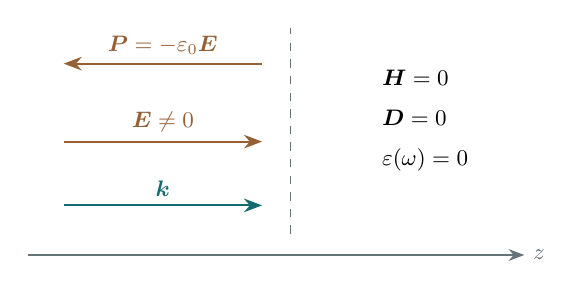
\begin{tikzpicture}[scale=.9,transform shape]
\draw[axis] (0,0)--(7,0) node[right] {$z$};
\draw[motion] (.5,.7)--(3.3,.7) node[midway,above] {$\boldsymbol k$};
\draw[force] (.5,1.6)--(3.3,1.6) node[midway,above] {$\boldsymbol E\ne0$};
\draw[force,color=warm] (3.3,2.7)--(.5,2.7) node[midway,above] {$\boldsymbol P=-\varepsilon_0\boldsymbol E$};
\node[align=left] at (5.6,1.9) {$\boldsymbol H=0$\\[5pt]$\boldsymbol D=0$\\[5pt]$\varepsilon(\omega)=0$};
\draw[guide] (3.7,.3)--(3.7,3.2);
\end{tikzpicture}
\figcaption{解图光5.7D\quad 纵向电场与极化相消给零电位移，磁场同时为零}
\end{minipage}\end{center}
在无碰撞、重离子固定的冷等离子体中，横向受迫响应所用的自由电子介电函数为$\varepsilon=1-\omega_p^2/\omega^2$，纵向模式取其零点，因此
\[
\boxed{\omega=\omega_p=\sqrt{\frac{Ne^2}{\varepsilon_0m_e}}}.
\]
用一维电子位移说明介电零点对应的实际运动。记位移为$\xi(z,t)$。粒子数守恒到一次给$\delta N=-N\partial_z\xi$，电子感应电荷为$\rho_{\rm ind}=-e\delta N=eN\partial_z\xi$。Gauss方程对非零波数的模式给
\[
\partial_zE=\frac{eN}{\varepsilon_0}\partial_z\xi
\quad\Longrightarrow\quad E=\frac{eN}{\varepsilon_0}\xi.
\]
空间常数场另属均匀外场分量；本题非零$k$的模式取上面的关系。电子方程$m_e\ddot\xi=-eE$随即成为$\ddot\xi+\omega_p^2\xi=0$。解图光5.7A取$\xi=\xi_0\cos(kz-\omega_pt)$，$E$与位移同相，电子所受力反向；压缩与稀疏由位移梯度决定。
\begin{center}\begin{minipage}{.98\linewidth}\centering
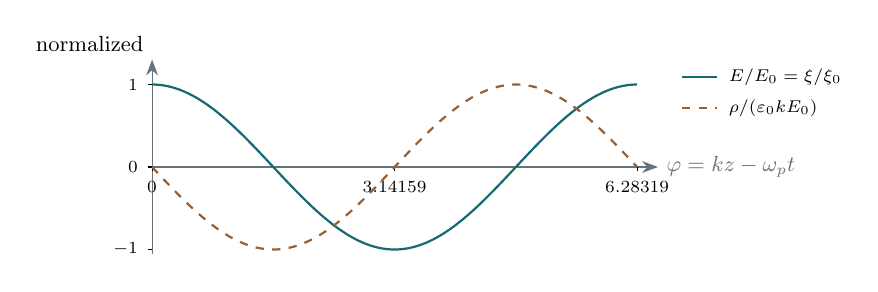
\begin{tikzpicture}[scale=.88,transform shape]
\draw[axis] (0,1.25)--(7.3,1.25) node[right] {$\varphi=kz-\omega_pt$};
\draw[axis] (0,0)--(0,2.8);
\node[above left] at (0,2.8) {$\mathrm{normalized}$};
\draw[thin] (0.000000,1.25)--(0.000000,1.19);\node[below,font=\scriptsize] at (0.000000,1.17) {$ 0 $};
\draw[thin] (3.500000,1.25)--(3.500000,1.19);\node[below,font=\scriptsize] at (3.500000,1.17) {$ 3.14159 $};
\draw[thin] (7.000000,1.25)--(7.000000,1.19);\node[below,font=\scriptsize] at (7.000000,1.17) {$ 6.28319 $};
\draw[thin] (0,0.059524)--(-.06,0.059524);\node[left,font=\scriptsize] at (-.08,0.059524) {$ -1 $};
\draw[thin] (0,1.250000)--(-.06,1.250000);\node[left,font=\scriptsize] at (-.08,1.250000) {$ 0 $};
\draw[thin] (0,2.440476)--(-.06,2.440476);\node[left,font=\scriptsize] at (-.08,2.440476) {$ 1 $};
\draw[thick,color=accent] plot coordinates {(0.0000000,2.4404762) (0.0291667,2.4400682) (0.0583333,2.4388447) (0.0875000,2.4368063) (0.1166667,2.4339546) (0.1458333,2.4302915) (0.1750000,2.4258195) (0.2041667,2.4205416) (0.2333333,2.4144614) (0.2625000,2.4075832) (0.2916667,2.3999117) (0.3208333,2.3914521) (0.3500000,2.3822101) (0.3791667,2.3721923) (0.4083333,2.3614053) (0.4375000,2.3498566) (0.4666667,2.3375541) (0.4958333,2.3245063) (0.5250000,2.3107221) (0.5541667,2.2962108) (0.5833333,2.2809826) (0.6125000,2.2650478) (0.6416667,2.2484173) (0.6708333,2.2311026) (0.7000000,2.2131155) (0.7291667,2.1944683) (0.7583333,2.1751738) (0.7875000,2.1552452) (0.8166667,2.1346962) (0.8458333,2.1135409) (0.8750000,2.0917938) (0.9041667,2.0694697) (0.9333333,2.0465841) (0.9625000,2.0231524) (0.9916667,1.9991909) (1.0208333,1.9747160) (1.0500000,1.9497443) (1.0791667,1.9242931) (1.1083333,1.8983798) (1.1375000,1.8720221) (1.1666667,1.8452381) (1.1958333,1.8180461) (1.2250000,1.7904649) (1.2541667,1.7625132) (1.2833333,1.7342103) (1.3125000,1.7055755) (1.3416667,1.6766285) (1.3708333,1.6473891) (1.4000000,1.6178774) (1.4291667,1.5881135) (1.4583333,1.5581179) (1.4875000,1.5279111) (1.5166667,1.4975139) (1.5458333,1.4669471) (1.5750000,1.4362315) (1.6041667,1.4053883) (1.6333333,1.3744386) (1.6625000,1.3434037) (1.6916667,1.3123047) (1.7208333,1.2811630) (1.7500000,1.2500000) (1.7791667,1.2188370) (1.8083333,1.1876953) (1.8375000,1.1565963) (1.8666667,1.1255614) (1.8958333,1.0946117) (1.9250000,1.0637685) (1.9541667,1.0330529) (1.9833333,1.0024861) (2.0125000,0.9720889) (2.0416667,0.9418821) (2.0708333,0.9118865) (2.1000000,0.8821226) (2.1291667,0.8526109) (2.1583333,0.8233715) (2.1875000,0.7944245) (2.2166667,0.7657897) (2.2458333,0.7374868) (2.2750000,0.7095351) (2.3041667,0.6819539) (2.3333333,0.6547619) (2.3625000,0.6279779) (2.3916667,0.6016202) (2.4208333,0.5757069) (2.4500000,0.5502557) (2.4791667,0.5252840) (2.5083333,0.5008091) (2.5375000,0.4768476) (2.5666667,0.4534159) (2.5958333,0.4305303) (2.6250000,0.4082062) (2.6541667,0.3864591) (2.6833333,0.3653038) (2.7125000,0.3447548) (2.7416667,0.3248262) (2.7708333,0.3055317) (2.8000000,0.2868845) (2.8291667,0.2688974) (2.8583333,0.2515827) (2.8875000,0.2349522) (2.9166667,0.2190174) (2.9458333,0.2037892) (2.9750000,0.1892779) (3.0041667,0.1754937) (3.0333333,0.1624459) (3.0625000,0.1501434) (3.0916667,0.1385947) (3.1208333,0.1278077) (3.1500000,0.1177899) (3.1791667,0.1085479) (3.2083333,0.1000883) (3.2375000,0.0924168) (3.2666667,0.0855386) (3.2958333,0.0794584) (3.3250000,0.0741805) (3.3541667,0.0697085) (3.3833333,0.0660454) (3.4125000,0.0631937) (3.4416667,0.0611553) (3.4708333,0.0599318) (3.5000000,0.0595238) (3.5291667,0.0599318) (3.5583333,0.0611553) (3.5875000,0.0631937) (3.6166667,0.0660454) (3.6458333,0.0697085) (3.6750000,0.0741805) (3.7041667,0.0794584) (3.7333333,0.0855386) (3.7625000,0.0924168) (3.7916667,0.1000883) (3.8208333,0.1085479) (3.8500000,0.1177899) (3.8791667,0.1278077) (3.9083333,0.1385947) (3.9375000,0.1501434) (3.9666667,0.1624459) (3.9958333,0.1754937) (4.0250000,0.1892779) (4.0541667,0.2037892) (4.0833333,0.2190174) (4.1125000,0.2349522) (4.1416667,0.2515827) (4.1708333,0.2688974) (4.2000000,0.2868845) (4.2291667,0.3055317) (4.2583333,0.3248262) (4.2875000,0.3447548) (4.3166667,0.3653038) (4.3458333,0.3864591) (4.3750000,0.4082062) (4.4041667,0.4305303) (4.4333333,0.4534159) (4.4625000,0.4768476) (4.4916667,0.5008091) (4.5208333,0.5252840) (4.5500000,0.5502557) (4.5791667,0.5757069) (4.6083333,0.6016202) (4.6375000,0.6279779) (4.6666667,0.6547619) (4.6958333,0.6819539) (4.7250000,0.7095351) (4.7541667,0.7374868) (4.7833333,0.7657897) (4.8125000,0.7944245) (4.8416667,0.8233715) (4.8708333,0.8526109) (4.9000000,0.8821226) (4.9291667,0.9118865) (4.9583333,0.9418821) (4.9875000,0.9720889) (5.0166667,1.0024861) (5.0458333,1.0330529) (5.0750000,1.0637685) (5.1041667,1.0946117) (5.1333333,1.1255614) (5.1625000,1.1565963) (5.1916667,1.1876953) (5.2208333,1.2188370) (5.2500000,1.2500000) (5.2791667,1.2811630) (5.3083333,1.3123047) (5.3375000,1.3434037) (5.3666667,1.3744386) (5.3958333,1.4053883) (5.4250000,1.4362315) (5.4541667,1.4669471) (5.4833333,1.4975139) (5.5125000,1.5279111) (5.5416667,1.5581179) (5.5708333,1.5881135) (5.6000000,1.6178774) (5.6291667,1.6473891) (5.6583333,1.6766285) (5.6875000,1.7055755) (5.7166667,1.7342103) (5.7458333,1.7625132) (5.7750000,1.7904649) (5.8041667,1.8180461) (5.8333333,1.8452381) (5.8625000,1.8720221) (5.8916667,1.8983798) (5.9208333,1.9242931) (5.9500000,1.9497443) (5.9791667,1.9747160) (6.0083333,1.9991909) (6.0375000,2.0231524) (6.0666667,2.0465841) (6.0958333,2.0694697) (6.1250000,2.0917938) (6.1541667,2.1135409) (6.1833333,2.1346962) (6.2125000,2.1552452) (6.2416667,2.1751738) (6.2708333,2.1944683) (6.3000000,2.2131155) (6.3291667,2.2311026) (6.3583333,2.2484173) (6.3875000,2.2650478) (6.4166667,2.2809826) (6.4458333,2.2962108) (6.4750000,2.3107221) (6.5041667,2.3245063) (6.5333333,2.3375541) (6.5625000,2.3498566) (6.5916667,2.3614053) (6.6208333,2.3721923) (6.6500000,2.3822101) (6.6791667,2.3914521) (6.7083333,2.3999117) (6.7375000,2.4075832) (6.7666667,2.4144614) (6.7958333,2.4205416) (6.8250000,2.4258195) (6.8541667,2.4302915) (6.8833333,2.4339546) (6.9125000,2.4368063) (6.9416667,2.4388447) (6.9708333,2.4400682) (7.0000000,2.4404762)};
\draw[thick,color=accent] (7.65,2.55)--(8.15,2.55);\node[right,font=\scriptsize] at (8.2,2.55) {$E/E_0=\xi/\xi_0$};
\draw[thick,dashed,color=warm] plot coordinates {(0.0000000,1.2500000) (0.0291667,1.2188370) (0.0583333,1.1876953) (0.0875000,1.1565963) (0.1166667,1.1255614) (0.1458333,1.0946117) (0.1750000,1.0637685) (0.2041667,1.0330529) (0.2333333,1.0024861) (0.2625000,0.9720889) (0.2916667,0.9418821) (0.3208333,0.9118865) (0.3500000,0.8821226) (0.3791667,0.8526109) (0.4083333,0.8233715) (0.4375000,0.7944245) (0.4666667,0.7657897) (0.4958333,0.7374868) (0.5250000,0.7095351) (0.5541667,0.6819539) (0.5833333,0.6547619) (0.6125000,0.6279779) (0.6416667,0.6016202) (0.6708333,0.5757069) (0.7000000,0.5502557) (0.7291667,0.5252840) (0.7583333,0.5008091) (0.7875000,0.4768476) (0.8166667,0.4534159) (0.8458333,0.4305303) (0.8750000,0.4082062) (0.9041667,0.3864591) (0.9333333,0.3653038) (0.9625000,0.3447548) (0.9916667,0.3248262) (1.0208333,0.3055317) (1.0500000,0.2868845) (1.0791667,0.2688974) (1.1083333,0.2515827) (1.1375000,0.2349522) (1.1666667,0.2190174) (1.1958333,0.2037892) (1.2250000,0.1892779) (1.2541667,0.1754937) (1.2833333,0.1624459) (1.3125000,0.1501434) (1.3416667,0.1385947) (1.3708333,0.1278077) (1.4000000,0.1177899) (1.4291667,0.1085479) (1.4583333,0.1000883) (1.4875000,0.0924168) (1.5166667,0.0855386) (1.5458333,0.0794584) (1.5750000,0.0741805) (1.6041667,0.0697085) (1.6333333,0.0660454) (1.6625000,0.0631937) (1.6916667,0.0611553) (1.7208333,0.0599318) (1.7500000,0.0595238) (1.7791667,0.0599318) (1.8083333,0.0611553) (1.8375000,0.0631937) (1.8666667,0.0660454) (1.8958333,0.0697085) (1.9250000,0.0741805) (1.9541667,0.0794584) (1.9833333,0.0855386) (2.0125000,0.0924168) (2.0416667,0.1000883) (2.0708333,0.1085479) (2.1000000,0.1177899) (2.1291667,0.1278077) (2.1583333,0.1385947) (2.1875000,0.1501434) (2.2166667,0.1624459) (2.2458333,0.1754937) (2.2750000,0.1892779) (2.3041667,0.2037892) (2.3333333,0.2190174) (2.3625000,0.2349522) (2.3916667,0.2515827) (2.4208333,0.2688974) (2.4500000,0.2868845) (2.4791667,0.3055317) (2.5083333,0.3248262) (2.5375000,0.3447548) (2.5666667,0.3653038) (2.5958333,0.3864591) (2.6250000,0.4082062) (2.6541667,0.4305303) (2.6833333,0.4534159) (2.7125000,0.4768476) (2.7416667,0.5008091) (2.7708333,0.5252840) (2.8000000,0.5502557) (2.8291667,0.5757069) (2.8583333,0.6016202) (2.8875000,0.6279779) (2.9166667,0.6547619) (2.9458333,0.6819539) (2.9750000,0.7095351) (3.0041667,0.7374868) (3.0333333,0.7657897) (3.0625000,0.7944245) (3.0916667,0.8233715) (3.1208333,0.8526109) (3.1500000,0.8821226) (3.1791667,0.9118865) (3.2083333,0.9418821) (3.2375000,0.9720889) (3.2666667,1.0024861) (3.2958333,1.0330529) (3.3250000,1.0637685) (3.3541667,1.0946117) (3.3833333,1.1255614) (3.4125000,1.1565963) (3.4416667,1.1876953) (3.4708333,1.2188370) (3.5000000,1.2500000) (3.5291667,1.2811630) (3.5583333,1.3123047) (3.5875000,1.3434037) (3.6166667,1.3744386) (3.6458333,1.4053883) (3.6750000,1.4362315) (3.7041667,1.4669471) (3.7333333,1.4975139) (3.7625000,1.5279111) (3.7916667,1.5581179) (3.8208333,1.5881135) (3.8500000,1.6178774) (3.8791667,1.6473891) (3.9083333,1.6766285) (3.9375000,1.7055755) (3.9666667,1.7342103) (3.9958333,1.7625132) (4.0250000,1.7904649) (4.0541667,1.8180461) (4.0833333,1.8452381) (4.1125000,1.8720221) (4.1416667,1.8983798) (4.1708333,1.9242931) (4.2000000,1.9497443) (4.2291667,1.9747160) (4.2583333,1.9991909) (4.2875000,2.0231524) (4.3166667,2.0465841) (4.3458333,2.0694697) (4.3750000,2.0917938) (4.4041667,2.1135409) (4.4333333,2.1346962) (4.4625000,2.1552452) (4.4916667,2.1751738) (4.5208333,2.1944683) (4.5500000,2.2131155) (4.5791667,2.2311026) (4.6083333,2.2484173) (4.6375000,2.2650478) (4.6666667,2.2809826) (4.6958333,2.2962108) (4.7250000,2.3107221) (4.7541667,2.3245063) (4.7833333,2.3375541) (4.8125000,2.3498566) (4.8416667,2.3614053) (4.8708333,2.3721923) (4.9000000,2.3822101) (4.9291667,2.3914521) (4.9583333,2.3999117) (4.9875000,2.4075832) (5.0166667,2.4144614) (5.0458333,2.4205416) (5.0750000,2.4258195) (5.1041667,2.4302915) (5.1333333,2.4339546) (5.1625000,2.4368063) (5.1916667,2.4388447) (5.2208333,2.4400682) (5.2500000,2.4404762) (5.2791667,2.4400682) (5.3083333,2.4388447) (5.3375000,2.4368063) (5.3666667,2.4339546) (5.3958333,2.4302915) (5.4250000,2.4258195) (5.4541667,2.4205416) (5.4833333,2.4144614) (5.5125000,2.4075832) (5.5416667,2.3999117) (5.5708333,2.3914521) (5.6000000,2.3822101) (5.6291667,2.3721923) (5.6583333,2.3614053) (5.6875000,2.3498566) (5.7166667,2.3375541) (5.7458333,2.3245063) (5.7750000,2.3107221) (5.8041667,2.2962108) (5.8333333,2.2809826) (5.8625000,2.2650478) (5.8916667,2.2484173) (5.9208333,2.2311026) (5.9500000,2.2131155) (5.9791667,2.1944683) (6.0083333,2.1751738) (6.0375000,2.1552452) (6.0666667,2.1346962) (6.0958333,2.1135409) (6.1250000,2.0917938) (6.1541667,2.0694697) (6.1833333,2.0465841) (6.2125000,2.0231524) (6.2416667,1.9991909) (6.2708333,1.9747160) (6.3000000,1.9497443) (6.3291667,1.9242931) (6.3583333,1.8983798) (6.3875000,1.8720221) (6.4166667,1.8452381) (6.4458333,1.8180461) (6.4750000,1.7904649) (6.5041667,1.7625132) (6.5333333,1.7342103) (6.5625000,1.7055755) (6.5916667,1.6766285) (6.6208333,1.6473891) (6.6500000,1.6178774) (6.6791667,1.5881135) (6.7083333,1.5581179) (6.7375000,1.5279111) (6.7666667,1.4975139) (6.7958333,1.4669471) (6.8250000,1.4362315) (6.8541667,1.4053883) (6.8833333,1.3744386) (6.9125000,1.3434037) (6.9416667,1.3123047) (6.9708333,1.2811630) (7.0000000,1.2500000)};
\draw[thick,dashed,color=warm] (7.65,2.0999999999999996)--(8.15,2.0999999999999996);\node[right,font=\scriptsize] at (8.2,2.0999999999999996) {$\rho/(\varepsilon_0 kE_0)$};
\end{tikzpicture}
\figcaption{解图光5.7A\quad 电场与电子位移同相；感应电荷由空间导数给出}
\end{minipage}\end{center}
感应电荷满足$\nabla\cdot\boldsymbol E=\rho_{\rm ind}/\varepsilon_0$。无外加自由电荷的宏观条件是$\nabla\cdot\boldsymbol D=0$，与这项内部感应电荷同时成立。相应的感应电流$J=-Ne\dot\xi$与真空位移电流相抵，$\boldsymbol H=0$正对应Ampere方程的零总旋度。

冷模型频率不依赖$k$，所以
\[
v_p=\frac{\omega_p}{k}\quad(k\ne0),\qquad
\boxed{v_g=\frac{\dd\omega}{\dd k}=0}.
\]
解图光5.7B将水平的纵向支与横向支$\omega_T^2=\omega_p^2+c^2k^2$画在一起。将第一个旋度式再与$\boldsymbol k$叉乘，并代入第二式，得
\[
 \boldsymbol k\times(\boldsymbol k\times\boldsymbol E)+\frac{\omega^2}{c^2}\varepsilon\boldsymbol E=0.
\]
写$\boldsymbol E=\boldsymbol E_L+\boldsymbol E_T$，其中$\boldsymbol E_L\parallel\boldsymbol k$、$\boldsymbol E_T\perp\boldsymbol k$。横向投影中$\boldsymbol k\times(\boldsymbol k\times\boldsymbol E_T)=-k^2\boldsymbol E_T$，于是$k^2=\varepsilon\omega^2/c^2$；纵向投影的叉乘项为零，非零$\omega,\boldsymbol E_L$给$\varepsilon=0$，允许任意非零$k$的空间相位分布。相位速度$\omega_p/k$描述这种分布的等相位位置，波包群速为零。
\begin{center}\begin{minipage}{.98\linewidth}\centering
\begin{tikzpicture}[scale=.88,transform shape]
\draw[axis] (0,0.0)--(7.3,0.0) node[right] {$ck/\omega_p$};
\draw[axis] (0,0)--(0,2.8);
\node[above left] at (0,2.8) {$\omega/\omega_p$};
\draw[thin] (0.000000,0.0)--(0.000000,-0.06);\node[below,font=\scriptsize] at (0.000000,-0.08) {$ 0 $};
\draw[thin] (2.333333,0.0)--(2.333333,-0.06);\node[below,font=\scriptsize] at (2.333333,-0.08) {$ 1 $};
\draw[thin] (4.666667,0.0)--(4.666667,-0.06);\node[below,font=\scriptsize] at (4.666667,-0.08) {$ 2 $};
\draw[thin] (7.000000,0.0)--(7.000000,-0.06);\node[below,font=\scriptsize] at (7.000000,-0.08) {$ 3 $};
\draw[thin] (0,0.000000)--(-.06,0.000000);\node[left,font=\scriptsize] at (-.08,0.000000) {$ 0 $};
\draw[thin] (0,0.757576)--(-.06,0.757576);\node[left,font=\scriptsize] at (-.08,0.757576) {$ 1 $};
\draw[thin] (0,1.515152)--(-.06,1.515152);\node[left,font=\scriptsize] at (-.08,1.515152) {$ 2 $};
\draw[thin] (0,2.272727)--(-.06,2.272727);\node[left,font=\scriptsize] at (-.08,2.272727) {$ 3 $};
\draw[thick,color=accent] plot coordinates {(0.0000000,0.7575758) (0.0291667,0.7575758) (0.0583333,0.7575758) (0.0875000,0.7575758) (0.1166667,0.7575758) (0.1458333,0.7575758) (0.1750000,0.7575758) (0.2041667,0.7575758) (0.2333333,0.7575758) (0.2625000,0.7575758) (0.2916667,0.7575758) (0.3208333,0.7575758) (0.3500000,0.7575758) (0.3791667,0.7575758) (0.4083333,0.7575758) (0.4375000,0.7575758) (0.4666667,0.7575758) (0.4958333,0.7575758) (0.5250000,0.7575758) (0.5541667,0.7575758) (0.5833333,0.7575758) (0.6125000,0.7575758) (0.6416667,0.7575758) (0.6708333,0.7575758) (0.7000000,0.7575758) (0.7291667,0.7575758) (0.7583333,0.7575758) (0.7875000,0.7575758) (0.8166667,0.7575758) (0.8458333,0.7575758) (0.8750000,0.7575758) (0.9041667,0.7575758) (0.9333333,0.7575758) (0.9625000,0.7575758) (0.9916667,0.7575758) (1.0208333,0.7575758) (1.0500000,0.7575758) (1.0791667,0.7575758) (1.1083333,0.7575758) (1.1375000,0.7575758) (1.1666667,0.7575758) (1.1958333,0.7575758) (1.2250000,0.7575758) (1.2541667,0.7575758) (1.2833333,0.7575758) (1.3125000,0.7575758) (1.3416667,0.7575758) (1.3708333,0.7575758) (1.4000000,0.7575758) (1.4291667,0.7575758) (1.4583333,0.7575758) (1.4875000,0.7575758) (1.5166667,0.7575758) (1.5458333,0.7575758) (1.5750000,0.7575758) (1.6041667,0.7575758) (1.6333333,0.7575758) (1.6625000,0.7575758) (1.6916667,0.7575758) (1.7208333,0.7575758) (1.7500000,0.7575758) (1.7791667,0.7575758) (1.8083333,0.7575758) (1.8375000,0.7575758) (1.8666667,0.7575758) (1.8958333,0.7575758) (1.9250000,0.7575758) (1.9541667,0.7575758) (1.9833333,0.7575758) (2.0125000,0.7575758) (2.0416667,0.7575758) (2.0708333,0.7575758) (2.1000000,0.7575758) (2.1291667,0.7575758) (2.1583333,0.7575758) (2.1875000,0.7575758) (2.2166667,0.7575758) (2.2458333,0.7575758) (2.2750000,0.7575758) (2.3041667,0.7575758) (2.3333333,0.7575758) (2.3625000,0.7575758) (2.3916667,0.7575758) (2.4208333,0.7575758) (2.4500000,0.7575758) (2.4791667,0.7575758) (2.5083333,0.7575758) (2.5375000,0.7575758) (2.5666667,0.7575758) (2.5958333,0.7575758) (2.6250000,0.7575758) (2.6541667,0.7575758) (2.6833333,0.7575758) (2.7125000,0.7575758) (2.7416667,0.7575758) (2.7708333,0.7575758) (2.8000000,0.7575758) (2.8291667,0.7575758) (2.8583333,0.7575758) (2.8875000,0.7575758) (2.9166667,0.7575758) (2.9458333,0.7575758) (2.9750000,0.7575758) (3.0041667,0.7575758) (3.0333333,0.7575758) (3.0625000,0.7575758) (3.0916667,0.7575758) (3.1208333,0.7575758) (3.1500000,0.7575758) (3.1791667,0.7575758) (3.2083333,0.7575758) (3.2375000,0.7575758) (3.2666667,0.7575758) (3.2958333,0.7575758) (3.3250000,0.7575758) (3.3541667,0.7575758) (3.3833333,0.7575758) (3.4125000,0.7575758) (3.4416667,0.7575758) (3.4708333,0.7575758) (3.5000000,0.7575758) (3.5291667,0.7575758) (3.5583333,0.7575758) (3.5875000,0.7575758) (3.6166667,0.7575758) (3.6458333,0.7575758) (3.6750000,0.7575758) (3.7041667,0.7575758) (3.7333333,0.7575758) (3.7625000,0.7575758) (3.7916667,0.7575758) (3.8208333,0.7575758) (3.8500000,0.7575758) (3.8791667,0.7575758) (3.9083333,0.7575758) (3.9375000,0.7575758) (3.9666667,0.7575758) (3.9958333,0.7575758) (4.0250000,0.7575758) (4.0541667,0.7575758) (4.0833333,0.7575758) (4.1125000,0.7575758) (4.1416667,0.7575758) (4.1708333,0.7575758) (4.2000000,0.7575758) (4.2291667,0.7575758) (4.2583333,0.7575758) (4.2875000,0.7575758) (4.3166667,0.7575758) (4.3458333,0.7575758) (4.3750000,0.7575758) (4.4041667,0.7575758) (4.4333333,0.7575758) (4.4625000,0.7575758) (4.4916667,0.7575758) (4.5208333,0.7575758) (4.5500000,0.7575758) (4.5791667,0.7575758) (4.6083333,0.7575758) (4.6375000,0.7575758) (4.6666667,0.7575758) (4.6958333,0.7575758) (4.7250000,0.7575758) (4.7541667,0.7575758) (4.7833333,0.7575758) (4.8125000,0.7575758) (4.8416667,0.7575758) (4.8708333,0.7575758) (4.9000000,0.7575758) (4.9291667,0.7575758) (4.9583333,0.7575758) (4.9875000,0.7575758) (5.0166667,0.7575758) (5.0458333,0.7575758) (5.0750000,0.7575758) (5.1041667,0.7575758) (5.1333333,0.7575758) (5.1625000,0.7575758) (5.1916667,0.7575758) (5.2208333,0.7575758) (5.2500000,0.7575758) (5.2791667,0.7575758) (5.3083333,0.7575758) (5.3375000,0.7575758) (5.3666667,0.7575758) (5.3958333,0.7575758) (5.4250000,0.7575758) (5.4541667,0.7575758) (5.4833333,0.7575758) (5.5125000,0.7575758) (5.5416667,0.7575758) (5.5708333,0.7575758) (5.6000000,0.7575758) (5.6291667,0.7575758) (5.6583333,0.7575758) (5.6875000,0.7575758) (5.7166667,0.7575758) (5.7458333,0.7575758) (5.7750000,0.7575758) (5.8041667,0.7575758) (5.8333333,0.7575758) (5.8625000,0.7575758) (5.8916667,0.7575758) (5.9208333,0.7575758) (5.9500000,0.7575758) (5.9791667,0.7575758) (6.0083333,0.7575758) (6.0375000,0.7575758) (6.0666667,0.7575758) (6.0958333,0.7575758) (6.1250000,0.7575758) (6.1541667,0.7575758) (6.1833333,0.7575758) (6.2125000,0.7575758) (6.2416667,0.7575758) (6.2708333,0.7575758) (6.3000000,0.7575758) (6.3291667,0.7575758) (6.3583333,0.7575758) (6.3875000,0.7575758) (6.4166667,0.7575758) (6.4458333,0.7575758) (6.4750000,0.7575758) (6.5041667,0.7575758) (6.5333333,0.7575758) (6.5625000,0.7575758) (6.5916667,0.7575758) (6.6208333,0.7575758) (6.6500000,0.7575758) (6.6791667,0.7575758) (6.7083333,0.7575758) (6.7375000,0.7575758) (6.7666667,0.7575758) (6.7958333,0.7575758) (6.8250000,0.7575758) (6.8541667,0.7575758) (6.8833333,0.7575758) (6.9125000,0.7575758) (6.9416667,0.7575758) (6.9708333,0.7575758) (7.0000000,0.7575758)};
\draw[thick,color=accent] (7.65,2.55)--(8.15,2.55);\node[right,font=\scriptsize] at (8.2,2.55) {$\omega_L/\omega_p$};
\draw[thick,dashed,color=warm] plot coordinates {(0.0000000,0.7575758) (0.0291667,0.7576349) (0.0583333,0.7578125) (0.0875000,0.7581082) (0.1166667,0.7585221) (0.1458333,0.7590540) (0.1750000,0.7597035) (0.2041667,0.7604703) (0.2333333,0.7613542) (0.2625000,0.7623547) (0.2916667,0.7634714) (0.3208333,0.7647037) (0.3500000,0.7660511) (0.3791667,0.7675130) (0.4083333,0.7690887) (0.4375000,0.7707775) (0.4666667,0.7725787) (0.4958333,0.7744915) (0.5250000,0.7765152) (0.5541667,0.7786487) (0.5833333,0.7808912) (0.6125000,0.7832418) (0.6416667,0.7856996) (0.6708333,0.7882634) (0.7000000,0.7909323) (0.7291667,0.7937052) (0.7583333,0.7965811) (0.7875000,0.7995588) (0.8166667,0.8026371) (0.8458333,0.8058150) (0.8750000,0.8090913) (0.9041667,0.8124647) (0.9333333,0.8159341) (0.9625000,0.8194982) (0.9916667,0.8231558) (1.0208333,0.8269057) (1.0500000,0.8307467) (1.0791667,0.8346774) (1.1083333,0.8386966) (1.1375000,0.8428030) (1.1666667,0.8469954) (1.1958333,0.8512726) (1.2250000,0.8556331) (1.2541667,0.8600758) (1.2833333,0.8645994) (1.3125000,0.8692026) (1.3416667,0.8738842) (1.3708333,0.8786430) (1.4000000,0.8834776) (1.4291667,0.8883868) (1.4583333,0.8933694) (1.4875000,0.8984242) (1.5166667,0.9035500) (1.5458333,0.9087456) (1.5750000,0.9140097) (1.6041667,0.9193413) (1.6333333,0.9247391) (1.6625000,0.9302019) (1.6916667,0.9357287) (1.7208333,0.9413184) (1.7500000,0.9469697) (1.7791667,0.9526816) (1.8083333,0.9584531) (1.8375000,0.9642830) (1.8666667,0.9701703) (1.8958333,0.9761140) (1.9250000,0.9821130) (1.9541667,0.9881664) (1.9833333,0.9942731) (2.0125000,1.0004321) (2.0416667,1.0066426) (2.0708333,1.0129035) (2.1000000,1.0192139) (2.1291667,1.0255730) (2.1583333,1.0319798) (2.1875000,1.0384333) (2.2166667,1.0449329) (2.2458333,1.0514776) (2.2750000,1.0580665) (2.3041667,1.0646989) (2.3333333,1.0713739) (2.3625000,1.0780908) (2.3916667,1.0848487) (2.4208333,1.0916470) (2.4500000,1.0984848) (2.4791667,1.1053615) (2.5083333,1.1122763) (2.5375000,1.1192284) (2.5666667,1.1262173) (2.5958333,1.1332422) (2.6250000,1.1403025) (2.6541667,1.1473975) (2.6833333,1.1545266) (2.7125000,1.1616891) (2.7416667,1.1688844) (2.7708333,1.1761120) (2.8000000,1.1833712) (2.8291667,1.1906614) (2.8583333,1.1979822) (2.8875000,1.2053328) (2.9166667,1.2127129) (2.9458333,1.2201219) (2.9750000,1.2275591) (3.0041667,1.2350242) (3.0333333,1.2425166) (3.0625000,1.2500359) (3.0916667,1.2575815) (3.1208333,1.2651529) (3.1500000,1.2727498) (3.1791667,1.2803717) (3.2083333,1.2880180) (3.2375000,1.2956885) (3.2666667,1.3033826) (3.2958333,1.3111000) (3.3250000,1.3188402) (3.3541667,1.3266028) (3.3833333,1.3343875) (3.4125000,1.3421938) (3.4416667,1.3500215) (3.4708333,1.3578700) (3.5000000,1.3657391) (3.5291667,1.3736284) (3.5583333,1.3815376) (3.5875000,1.3894663) (3.6166667,1.3974141) (3.6458333,1.4053809) (3.6750000,1.4133662) (3.7041667,1.4213697) (3.7333333,1.4293911) (3.7625000,1.4374301) (3.7916667,1.4454865) (3.8208333,1.4535599) (3.8500000,1.4616501) (3.8791667,1.4697568) (3.9083333,1.4778796) (3.9375000,1.4860184) (3.9666667,1.4941729) (3.9958333,1.5023429) (4.0250000,1.5105280) (4.0541667,1.5187280) (4.0833333,1.5269428) (4.1125000,1.5351719) (4.1416667,1.5434154) (4.1708333,1.5516728) (4.2000000,1.5599440) (4.2291667,1.5682287) (4.2583333,1.5765268) (4.2875000,1.5848380) (4.3166667,1.5931622) (4.3458333,1.6014991) (4.3750000,1.6098485) (4.4041667,1.6182102) (4.4333333,1.6265841) (4.4625000,1.6349700) (4.4916667,1.6433676) (4.5208333,1.6517769) (4.5500000,1.6601975) (4.5791667,1.6686294) (4.6083333,1.6770724) (4.6375000,1.6855263) (4.6666667,1.6939909) (4.6958333,1.7024661) (4.7250000,1.7109518) (4.7541667,1.7194477) (4.7833333,1.7279537) (4.8125000,1.7364698) (4.8416667,1.7449956) (4.8708333,1.7535312) (4.9000000,1.7620763) (4.9291667,1.7706308) (4.9583333,1.7791945) (4.9875000,1.7877674) (5.0166667,1.7963493) (5.0458333,1.8049401) (5.0750000,1.8135397) (5.1041667,1.8221479) (5.1333333,1.8307645) (5.1625000,1.8393896) (5.1916667,1.8480229) (5.2208333,1.8566644) (5.2500000,1.8653140) (5.2791667,1.8739714) (5.3083333,1.8826367) (5.3375000,1.8913097) (5.3666667,1.8999903) (5.3958333,1.9086784) (5.4250000,1.9173740) (5.4541667,1.9260768) (5.4833333,1.9347868) (5.5125000,1.9435039) (5.5416667,1.9522280) (5.5708333,1.9609591) (5.6000000,1.9696970) (5.6291667,1.9784416) (5.6583333,1.9871928) (5.6875000,1.9959507) (5.7166667,2.0047149) (5.7458333,2.0134856) (5.7750000,2.0222626) (5.8041667,2.0310458) (5.8333333,2.0398352) (5.8625000,2.0486306) (5.8916667,2.0574320) (5.9208333,2.0662393) (5.9500000,2.0750524) (5.9791667,2.0838713) (6.0083333,2.0926959) (6.0375000,2.1015261) (6.0666667,2.1103619) (6.0958333,2.1192031) (6.1250000,2.1280497) (6.1541667,2.1369017) (6.1833333,2.1457589) (6.2125000,2.1546214) (6.2416667,2.1634890) (6.2708333,2.1723617) (6.3000000,2.1812394) (6.3291667,2.1901221) (6.3583333,2.1990096) (6.3875000,2.2079020) (6.4166667,2.2167992) (6.4458333,2.2257011) (6.4750000,2.2346077) (6.5041667,2.2435189) (6.5333333,2.2524347) (6.5625000,2.2613549) (6.5916667,2.2702796) (6.6208333,2.2792087) (6.6500000,2.2881422) (6.6791667,2.2970799) (6.7083333,2.3060219) (6.7375000,2.3149681) (6.7666667,2.3239184) (6.7958333,2.3328729) (6.8250000,2.3418314) (6.8541667,2.3507939) (6.8833333,2.3597603) (6.9125000,2.3687307) (6.9416667,2.3777050) (6.9708333,2.3866830) (7.0000000,2.3956649)};
\draw[thick,dashed,color=warm] (7.65,2.0999999999999996)--(8.15,2.0999999999999996);\node[right,font=\scriptsize] at (8.2,2.0999999999999996) {$\omega_T/\omega_p$};
\end{tikzpicture}
\figcaption{解图光5.7B\quad 冷纵向水平支与横向传播支使用各自的场投影}
\end{minipage}\end{center}
能量可直接由电子运动说明。位移振幅为$\xi_0$，$E_0=eN\xi_0/\varepsilon_0$，在固定位置的一个振荡周期中，电场能和电子动能为
\[
 u_E=\frac{\varepsilon_0E_0^2}{2}\cos^2\varphi,\qquad
 u_k=\frac{Nm_e\omega_p^2\xi_0^2}{2}\sin^2\varphi,
 \quad\varphi=kz-\omega_pt.
\]
两系数相同，故总能量密度$U=\varepsilon_0E_0^2/2$，时间平均两份各为$\varepsilon_0E_0^2/4$。解图光5.7C画出这项往返交换，电磁Poynting流$\boldsymbol E\times\boldsymbol H=0$。在当前冷、无空间色散模型中，局部能量在场与电子动能间交换，包络保持原来的空间位置。
\begin{center}\begin{minipage}{.98\linewidth}\centering
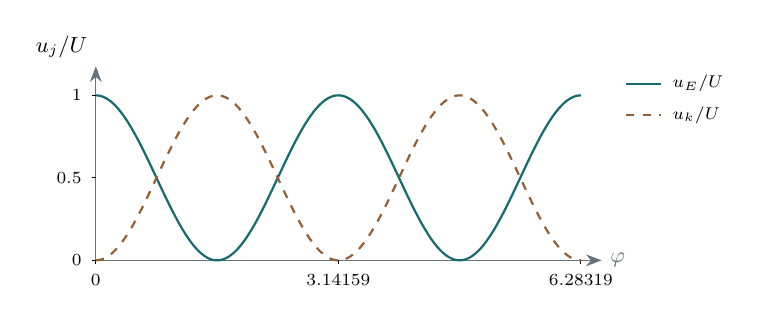
\begin{tikzpicture}[scale=.88,transform shape]
\draw[axis] (0,0.0)--(7.3,0.0) node[right] {$\varphi$};
\draw[axis] (0,0)--(0,2.8);
\node[above left] at (0,2.8) {$u_j/U$};
\draw[thin] (0.000000,0.0)--(0.000000,-0.06);\node[below,font=\scriptsize] at (0.000000,-0.08) {$ 0 $};
\draw[thin] (3.500000,0.0)--(3.500000,-0.06);\node[below,font=\scriptsize] at (3.500000,-0.08) {$ 3.14159 $};
\draw[thin] (7.000000,0.0)--(7.000000,-0.06);\node[below,font=\scriptsize] at (7.000000,-0.08) {$ 6.28319 $};
\draw[thin] (0,0.000000)--(-.06,0.000000);\node[left,font=\scriptsize] at (-.08,0.000000) {$ 0 $};
\draw[thin] (0,1.190476)--(-.06,1.190476);\node[left,font=\scriptsize] at (-.08,1.190476) {$ 0.5 $};
\draw[thin] (0,2.380952)--(-.06,2.380952);\node[left,font=\scriptsize] at (-.08,2.380952) {$ 1 $};
\draw[thick,color=accent] plot coordinates {(0.0000000,2.3809524) (0.0291667,2.3793209) (0.0583333,2.3744308) (0.0875000,2.3662956) (0.1166667,2.3549376) (0.1458333,2.3403879) (0.1750000,2.3226863) (0.2041667,2.3018815) (0.2333333,2.2780303) (0.2625000,2.2511982) (0.2916667,2.2214588) (0.3208333,2.1888935) (0.3500000,2.1535917) (0.3791667,2.1156500) (0.4083333,2.0751724) (0.4375000,2.0322700) (0.4666667,1.9870602) (0.4958333,1.9396671) (0.5250000,1.8902205) (0.5541667,1.8388560) (0.5833333,1.7857143) (0.6125000,1.7309411) (0.6416667,1.6746865) (0.6708333,1.6171047) (0.7000000,1.5583536) (0.7291667,1.4985941) (0.7583333,1.4379901) (0.7875000,1.3767077) (0.8166667,1.3149148) (0.8458333,1.2527809) (0.8750000,1.1904762) (0.9041667,1.1281715) (0.9333333,1.0660375) (0.9625000,1.0042447) (0.9916667,0.9429623) (1.0208333,0.8823583) (1.0500000,0.8225988) (1.0791667,0.7638477) (1.1083333,0.7062659) (1.1375000,0.6500113) (1.1666667,0.5952381) (1.1958333,0.5420964) (1.2250000,0.4907318) (1.2541667,0.4412852) (1.2833333,0.3938921) (1.3125000,0.3486824) (1.3416667,0.3057800) (1.3708333,0.2653024) (1.4000000,0.2273607) (1.4291667,0.1920588) (1.4583333,0.1594936) (1.4875000,0.1297541) (1.5166667,0.1029221) (1.5458333,0.0790709) (1.5750000,0.0582661) (1.6041667,0.0405645) (1.6333333,0.0260148) (1.6625000,0.0146567) (1.6916667,0.0065216) (1.7208333,0.0016315) (1.7500000,0.0000000) (1.7791667,0.0016315) (1.8083333,0.0065216) (1.8375000,0.0146567) (1.8666667,0.0260148) (1.8958333,0.0405645) (1.9250000,0.0582661) (1.9541667,0.0790709) (1.9833333,0.1029221) (2.0125000,0.1297541) (2.0416667,0.1594936) (2.0708333,0.1920588) (2.1000000,0.2273607) (2.1291667,0.2653024) (2.1583333,0.3057800) (2.1875000,0.3486824) (2.2166667,0.3938921) (2.2458333,0.4412852) (2.2750000,0.4907318) (2.3041667,0.5420964) (2.3333333,0.5952381) (2.3625000,0.6500113) (2.3916667,0.7062659) (2.4208333,0.7638477) (2.4500000,0.8225988) (2.4791667,0.8823583) (2.5083333,0.9429623) (2.5375000,1.0042447) (2.5666667,1.0660375) (2.5958333,1.1281715) (2.6250000,1.1904762) (2.6541667,1.2527809) (2.6833333,1.3149148) (2.7125000,1.3767077) (2.7416667,1.4379901) (2.7708333,1.4985941) (2.8000000,1.5583536) (2.8291667,1.6171047) (2.8583333,1.6746865) (2.8875000,1.7309411) (2.9166667,1.7857143) (2.9458333,1.8388560) (2.9750000,1.8902205) (3.0041667,1.9396671) (3.0333333,1.9870602) (3.0625000,2.0322700) (3.0916667,2.0751724) (3.1208333,2.1156500) (3.1500000,2.1535917) (3.1791667,2.1888935) (3.2083333,2.2214588) (3.2375000,2.2511982) (3.2666667,2.2780303) (3.2958333,2.3018815) (3.3250000,2.3226863) (3.3541667,2.3403879) (3.3833333,2.3549376) (3.4125000,2.3662956) (3.4416667,2.3744308) (3.4708333,2.3793209) (3.5000000,2.3809524) (3.5291667,2.3793209) (3.5583333,2.3744308) (3.5875000,2.3662956) (3.6166667,2.3549376) (3.6458333,2.3403879) (3.6750000,2.3226863) (3.7041667,2.3018815) (3.7333333,2.2780303) (3.7625000,2.2511982) (3.7916667,2.2214588) (3.8208333,2.1888935) (3.8500000,2.1535917) (3.8791667,2.1156500) (3.9083333,2.0751724) (3.9375000,2.0322700) (3.9666667,1.9870602) (3.9958333,1.9396671) (4.0250000,1.8902205) (4.0541667,1.8388560) (4.0833333,1.7857143) (4.1125000,1.7309411) (4.1416667,1.6746865) (4.1708333,1.6171047) (4.2000000,1.5583536) (4.2291667,1.4985941) (4.2583333,1.4379901) (4.2875000,1.3767077) (4.3166667,1.3149148) (4.3458333,1.2527809) (4.3750000,1.1904762) (4.4041667,1.1281715) (4.4333333,1.0660375) (4.4625000,1.0042447) (4.4916667,0.9429623) (4.5208333,0.8823583) (4.5500000,0.8225988) (4.5791667,0.7638477) (4.6083333,0.7062659) (4.6375000,0.6500113) (4.6666667,0.5952381) (4.6958333,0.5420964) (4.7250000,0.4907318) (4.7541667,0.4412852) (4.7833333,0.3938921) (4.8125000,0.3486824) (4.8416667,0.3057800) (4.8708333,0.2653024) (4.9000000,0.2273607) (4.9291667,0.1920588) (4.9583333,0.1594936) (4.9875000,0.1297541) (5.0166667,0.1029221) (5.0458333,0.0790709) (5.0750000,0.0582661) (5.1041667,0.0405645) (5.1333333,0.0260148) (5.1625000,0.0146567) (5.1916667,0.0065216) (5.2208333,0.0016315) (5.2500000,0.0000000) (5.2791667,0.0016315) (5.3083333,0.0065216) (5.3375000,0.0146567) (5.3666667,0.0260148) (5.3958333,0.0405645) (5.4250000,0.0582661) (5.4541667,0.0790709) (5.4833333,0.1029221) (5.5125000,0.1297541) (5.5416667,0.1594936) (5.5708333,0.1920588) (5.6000000,0.2273607) (5.6291667,0.2653024) (5.6583333,0.3057800) (5.6875000,0.3486824) (5.7166667,0.3938921) (5.7458333,0.4412852) (5.7750000,0.4907318) (5.8041667,0.5420964) (5.8333333,0.5952381) (5.8625000,0.6500113) (5.8916667,0.7062659) (5.9208333,0.7638477) (5.9500000,0.8225988) (5.9791667,0.8823583) (6.0083333,0.9429623) (6.0375000,1.0042447) (6.0666667,1.0660375) (6.0958333,1.1281715) (6.1250000,1.1904762) (6.1541667,1.2527809) (6.1833333,1.3149148) (6.2125000,1.3767077) (6.2416667,1.4379901) (6.2708333,1.4985941) (6.3000000,1.5583536) (6.3291667,1.6171047) (6.3583333,1.6746865) (6.3875000,1.7309411) (6.4166667,1.7857143) (6.4458333,1.8388560) (6.4750000,1.8902205) (6.5041667,1.9396671) (6.5333333,1.9870602) (6.5625000,2.0322700) (6.5916667,2.0751724) (6.6208333,2.1156500) (6.6500000,2.1535917) (6.6791667,2.1888935) (6.7083333,2.2214588) (6.7375000,2.2511982) (6.7666667,2.2780303) (6.7958333,2.3018815) (6.8250000,2.3226863) (6.8541667,2.3403879) (6.8833333,2.3549376) (6.9125000,2.3662956) (6.9416667,2.3744308) (6.9708333,2.3793209) (7.0000000,2.3809524)};
\draw[thick,color=accent] (7.65,2.55)--(8.15,2.55);\node[right,font=\scriptsize] at (8.2,2.55) {$u_E/U$};
\draw[thick,dashed,color=warm] plot coordinates {(0.0000000,0.0000000) (0.0291667,0.0016315) (0.0583333,0.0065216) (0.0875000,0.0146567) (0.1166667,0.0260148) (0.1458333,0.0405645) (0.1750000,0.0582661) (0.2041667,0.0790709) (0.2333333,0.1029221) (0.2625000,0.1297541) (0.2916667,0.1594936) (0.3208333,0.1920588) (0.3500000,0.2273607) (0.3791667,0.2653024) (0.4083333,0.3057800) (0.4375000,0.3486824) (0.4666667,0.3938921) (0.4958333,0.4412852) (0.5250000,0.4907318) (0.5541667,0.5420964) (0.5833333,0.5952381) (0.6125000,0.6500113) (0.6416667,0.7062659) (0.6708333,0.7638477) (0.7000000,0.8225988) (0.7291667,0.8823583) (0.7583333,0.9429623) (0.7875000,1.0042447) (0.8166667,1.0660375) (0.8458333,1.1281715) (0.8750000,1.1904762) (0.9041667,1.2527809) (0.9333333,1.3149148) (0.9625000,1.3767077) (0.9916667,1.4379901) (1.0208333,1.4985941) (1.0500000,1.5583536) (1.0791667,1.6171047) (1.1083333,1.6746865) (1.1375000,1.7309411) (1.1666667,1.7857143) (1.1958333,1.8388560) (1.2250000,1.8902205) (1.2541667,1.9396671) (1.2833333,1.9870602) (1.3125000,2.0322700) (1.3416667,2.0751724) (1.3708333,2.1156500) (1.4000000,2.1535917) (1.4291667,2.1888935) (1.4583333,2.2214588) (1.4875000,2.2511982) (1.5166667,2.2780303) (1.5458333,2.3018815) (1.5750000,2.3226863) (1.6041667,2.3403879) (1.6333333,2.3549376) (1.6625000,2.3662956) (1.6916667,2.3744308) (1.7208333,2.3793209) (1.7500000,2.3809524) (1.7791667,2.3793209) (1.8083333,2.3744308) (1.8375000,2.3662956) (1.8666667,2.3549376) (1.8958333,2.3403879) (1.9250000,2.3226863) (1.9541667,2.3018815) (1.9833333,2.2780303) (2.0125000,2.2511982) (2.0416667,2.2214588) (2.0708333,2.1888935) (2.1000000,2.1535917) (2.1291667,2.1156500) (2.1583333,2.0751724) (2.1875000,2.0322700) (2.2166667,1.9870602) (2.2458333,1.9396671) (2.2750000,1.8902205) (2.3041667,1.8388560) (2.3333333,1.7857143) (2.3625000,1.7309411) (2.3916667,1.6746865) (2.4208333,1.6171047) (2.4500000,1.5583536) (2.4791667,1.4985941) (2.5083333,1.4379901) (2.5375000,1.3767077) (2.5666667,1.3149148) (2.5958333,1.2527809) (2.6250000,1.1904762) (2.6541667,1.1281715) (2.6833333,1.0660375) (2.7125000,1.0042447) (2.7416667,0.9429623) (2.7708333,0.8823583) (2.8000000,0.8225988) (2.8291667,0.7638477) (2.8583333,0.7062659) (2.8875000,0.6500113) (2.9166667,0.5952381) (2.9458333,0.5420964) (2.9750000,0.4907318) (3.0041667,0.4412852) (3.0333333,0.3938921) (3.0625000,0.3486824) (3.0916667,0.3057800) (3.1208333,0.2653024) (3.1500000,0.2273607) (3.1791667,0.1920588) (3.2083333,0.1594936) (3.2375000,0.1297541) (3.2666667,0.1029221) (3.2958333,0.0790709) (3.3250000,0.0582661) (3.3541667,0.0405645) (3.3833333,0.0260148) (3.4125000,0.0146567) (3.4416667,0.0065216) (3.4708333,0.0016315) (3.5000000,0.0000000) (3.5291667,0.0016315) (3.5583333,0.0065216) (3.5875000,0.0146567) (3.6166667,0.0260148) (3.6458333,0.0405645) (3.6750000,0.0582661) (3.7041667,0.0790709) (3.7333333,0.1029221) (3.7625000,0.1297541) (3.7916667,0.1594936) (3.8208333,0.1920588) (3.8500000,0.2273607) (3.8791667,0.2653024) (3.9083333,0.3057800) (3.9375000,0.3486824) (3.9666667,0.3938921) (3.9958333,0.4412852) (4.0250000,0.4907318) (4.0541667,0.5420964) (4.0833333,0.5952381) (4.1125000,0.6500113) (4.1416667,0.7062659) (4.1708333,0.7638477) (4.2000000,0.8225988) (4.2291667,0.8823583) (4.2583333,0.9429623) (4.2875000,1.0042447) (4.3166667,1.0660375) (4.3458333,1.1281715) (4.3750000,1.1904762) (4.4041667,1.2527809) (4.4333333,1.3149148) (4.4625000,1.3767077) (4.4916667,1.4379901) (4.5208333,1.4985941) (4.5500000,1.5583536) (4.5791667,1.6171047) (4.6083333,1.6746865) (4.6375000,1.7309411) (4.6666667,1.7857143) (4.6958333,1.8388560) (4.7250000,1.8902205) (4.7541667,1.9396671) (4.7833333,1.9870602) (4.8125000,2.0322700) (4.8416667,2.0751724) (4.8708333,2.1156500) (4.9000000,2.1535917) (4.9291667,2.1888935) (4.9583333,2.2214588) (4.9875000,2.2511982) (5.0166667,2.2780303) (5.0458333,2.3018815) (5.0750000,2.3226863) (5.1041667,2.3403879) (5.1333333,2.3549376) (5.1625000,2.3662956) (5.1916667,2.3744308) (5.2208333,2.3793209) (5.2500000,2.3809524) (5.2791667,2.3793209) (5.3083333,2.3744308) (5.3375000,2.3662956) (5.3666667,2.3549376) (5.3958333,2.3403879) (5.4250000,2.3226863) (5.4541667,2.3018815) (5.4833333,2.2780303) (5.5125000,2.2511982) (5.5416667,2.2214588) (5.5708333,2.1888935) (5.6000000,2.1535917) (5.6291667,2.1156500) (5.6583333,2.0751724) (5.6875000,2.0322700) (5.7166667,1.9870602) (5.7458333,1.9396671) (5.7750000,1.8902205) (5.8041667,1.8388560) (5.8333333,1.7857143) (5.8625000,1.7309411) (5.8916667,1.6746865) (5.9208333,1.6171047) (5.9500000,1.5583536) (5.9791667,1.4985941) (6.0083333,1.4379901) (6.0375000,1.3767077) (6.0666667,1.3149148) (6.0958333,1.2527809) (6.1250000,1.1904762) (6.1541667,1.1281715) (6.1833333,1.0660375) (6.2125000,1.0042447) (6.2416667,0.9429623) (6.2708333,0.8823583) (6.3000000,0.8225988) (6.3291667,0.7638477) (6.3583333,0.7062659) (6.3875000,0.6500113) (6.4166667,0.5952381) (6.4458333,0.5420964) (6.4750000,0.4907318) (6.5041667,0.4412852) (6.5333333,0.3938921) (6.5625000,0.3486824) (6.5916667,0.3057800) (6.6208333,0.2653024) (6.6500000,0.2273607) (6.6791667,0.1920588) (6.7083333,0.1594936) (6.7375000,0.1297541) (6.7666667,0.1029221) (6.7958333,0.0790709) (6.8250000,0.0582661) (6.8541667,0.0405645) (6.8833333,0.0260148) (6.9125000,0.0146567) (6.9416667,0.0065216) (6.9708333,0.0016315) (7.0000000,0.0000000)};
\draw[thick,dashed,color=warm] (7.65,2.0999999999999996)--(8.15,2.0999999999999996);\node[right,font=\scriptsize] at (8.2,2.0999999999999996) {$u_k/U$};
\end{tikzpicture}
\figcaption{解图光5.7C\quad 固定位置的电场能与电子动能往返交换，总量U不变}
\end{minipage}\end{center}
加入电子压力后，位移方程增加空间梯度项，频率成为$\omega^2=\omega_p^2+u^2k^2$，群速度相应非零；其中的能量传输还包含电子压力的机械功率。冷模型给出零群速和局部能量交换；加入压力后，用纵向场方程与指定的压力闭合共同求频率和能流。


\Needspace{13\baselineskip}

\pdfbookmark[2]{第 8 题 均匀介质与涨落散射}{q8}

\section*{第 8 题\quad 均匀介质与涨落散射}\label{q:8}

根据经典电磁理论，说明无限均匀、无密度涨落的介质为何没有偏离前向的体散射；再把介质分为许多尺寸远小于波长的微元，设微元响应振幅相对均值的涨落为$\Delta A_j$，证明在互不相关的零均值涨落条件下，平均散射强度与$\langle|\Delta A|^2\rangle$成正比。说明样品的有限尺寸及空间相关会怎样改变论证。

\begin{center}\begin{minipage}{.98\linewidth}\centering
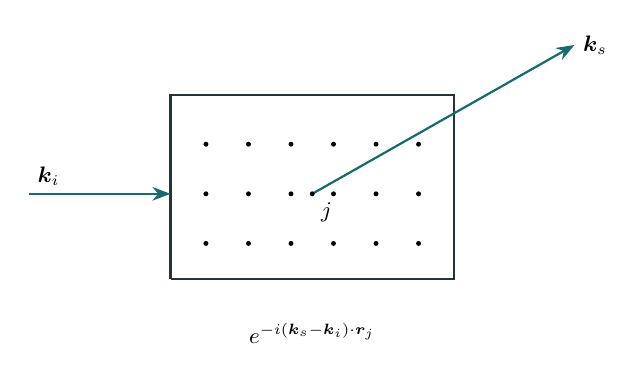
\begin{tikzpicture}[scale=.9,transform shape]
\draw[object] (0.00000,-1.00000)--(4.00000,-1.00000)--(4.00000,1.60000)--(0.00000,1.60000)--(0.00000,-1.00000);\fill (0.50000,-0.50000) circle(.035);\fill (0.50000,0.20000) circle(.035);\fill (0.50000,0.90000) circle(.035);\fill (1.10000,-0.50000) circle(.035);\fill (1.10000,0.20000) circle(.035);\fill (1.10000,0.90000) circle(.035);\fill (1.70000,-0.50000) circle(.035);\fill (1.70000,0.20000) circle(.035);\fill (1.70000,0.90000) circle(.035);\fill (2.30000,-0.50000) circle(.035);\fill (2.30000,0.20000) circle(.035);\fill (2.30000,0.90000) circle(.035);\fill (2.90000,-0.50000) circle(.035);\fill (2.90000,0.20000) circle(.035);\fill (2.90000,0.90000) circle(.035);\fill (3.50000,-0.50000) circle(.035);\fill (3.50000,0.20000) circle(.035);\fill (3.50000,0.90000) circle(.035);\draw[motion] (-2.00000,0.20000)--(0.00000,0.20000);\node[above right] at (-2.00000,0.20000) {$\boldsymbol k_i$};\draw[motion] (2.00000,0.20000)--(5.70000,2.30000);\node[right] at (5.70000,2.30000) {$\boldsymbol k_s$};\fill (2.00000,0.20000) circle(.035);\node[below right] at (2.00000,0.20000) {$j$};\node[below] at (2.00000,-1.50000) {$e^{-i(\boldsymbol k_s-\boldsymbol k_i)\cdot\boldsymbol r_j}$};
\end{tikzpicture}
\figcaption{图光5.8\quad 每个微元的相位由入射与出射方向共同决定。}
\end{minipage}\end{center}

\Needspace{6\baselineskip}\subsection*{解答}


图光5.8以$\boldsymbol k_i$标入射方向，$\boldsymbol k_s$标远场观察方向。各微元线度远小于波长，在微元内部可用同一偶极相位；不同微元之间保留位置造成的相位差。在线性、单次散射近似下，偶极响应沿入射场方向，次波的方向因子和观察距离取共同因子，以下先计算空间振幅。

位于$\boldsymbol r_j$的微元受迫相位为$\boldsymbol k_i\cdot\boldsymbol r_j$。观察点足够远时，传播距离为$r-\hat{\boldsymbol s}\cdot\boldsymbol r_j$，去掉所有项共有的$e^{ikr}/r$后，剩下
\[
e^{i(\boldsymbol k_i-\boldsymbol k_s)\cdot\boldsymbol r_j}
=e^{-i\boldsymbol q\cdot\boldsymbol r_j},\qquad
\boldsymbol q=\boldsymbol k_s-\boldsymbol k_i.
\]
解图光5.8D画出同一微元的入射、出射两段路径和波矢差。对于确定的位置，几何相位是确定的；空间排列与观察方向共同决定其相干和。弹性散射使$|\boldsymbol k_s|=|\boldsymbol k_i|=k$。D图右侧的两个等长波矢给出$\boldsymbol q$；若两波矢夹角为$\theta$，则$q=2k\sin(\theta/2)$。
\begin{center}\begin{minipage}{.98\linewidth}\centering
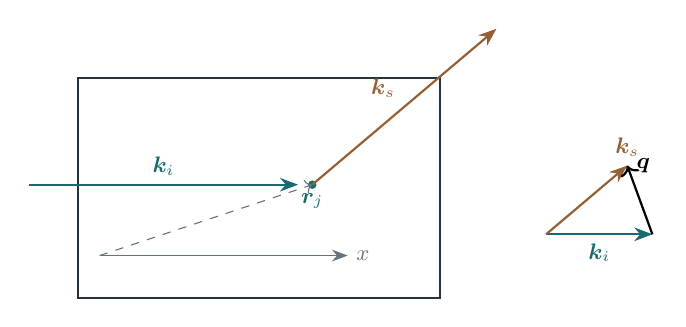
\begin{tikzpicture}[scale=.9,transform shape]
\coordinate (O) at (0,0);\coordinate (M) at (3,1);
\draw[object] (-.3,-.6) rectangle (4.8,2.5);
\fill[color=accent] (M) circle(.06) node[below] {$\boldsymbol r_j$};
\draw[motion] (-1,1)--(2.8,1) node[midway,above] {$\boldsymbol k_i$};
\draw[force] (M)--(5.6,3.2) node[midway,above left] {$\boldsymbol k_s$};
\draw[axis] (O)--(3.5,0) node[right] {$x$};
\draw[guide,->] (O)--(M);
\draw[motion] (6.3,.3)--(7.8,.3) node[midway,below] {$\boldsymbol k_i$};
\draw[force] (6.3,.3)--(7.445079428,1.268913362) node[above] {$\boldsymbol k_s$};
\draw[->,thick] (7.8,.3)--(7.445079428,1.268913362) node[right] {$\boldsymbol q$};
\end{tikzpicture}
\figcaption{解图光5.8D\quad 同一微元的激励和辐射传播共同给出负波矢转移相位}
\end{minipage}\end{center}
均匀连续介质的响应密度为$\chi_0$，微元振幅为$\chi_0\dd^3r$。将微元相干相加，得到
\[
F_0(\boldsymbol q)=\chi_0\int_V e^{-i\boldsymbol q\cdot\boldsymbol r}\dd^3r.
\]
取长方体中心为坐标原点，对每个坐标分别积分：
\[
 \int_{-L_\alpha/2}^{L_\alpha/2}e^{-iq_\alpha x_\alpha}\dd x_\alpha
 =L_\alpha\frac{\sin(q_\alpha L_\alpha/2)}{q_\alpha L_\alpha/2}.
\]
因三维积分可分离，
\[
F_0=\chi_0 V\prod_{\alpha=x,y,z}\operatorname{sinc}(q_\alpha L_\alpha/2),
\qquad \operatorname{sinc}u=\frac{\sin u}{u}.
\]
解图光5.8A取另两方向的$q$分量为零，画$|F_0/(\chi_0V)|^2$。峰宽随样品长度增大而缩小，第一零点为$|q_x|=2\pi/L_x$；有限样品的外形产生衍射。无限均匀连续体的Fourier谱集中在$\boldsymbol q=0$，故只有前向相干响应，偏离前向的体散射为零。均匀极化同时进入折射率，决定介质中的传播相位。
\begin{center}\begin{minipage}{.98\linewidth}\centering
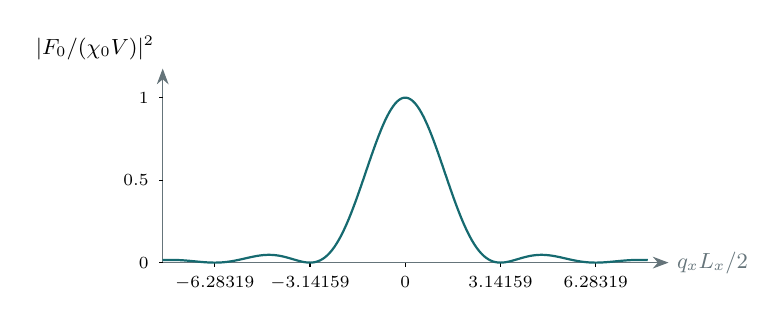
\begin{tikzpicture}[scale=.88,transform shape]
\draw[axis] (0,0.0)--(7.3,0.0) node[right] {$q_xL_x/2$};
\draw[axis] (0,0)--(0,2.8);
\node[above left] at (0,2.8) {$|F_0/(\chi_0V)|^2$};
\draw[thin] (0.751104,0.0)--(0.751104,-0.06);\node[below,font=\scriptsize] at (0.751104,-0.08) {$ -6.28319 $};
\draw[thin] (2.125554,0.0)--(2.125554,-0.06);\node[below,font=\scriptsize] at (2.125554,-0.08) {$ -3.14159 $};
\draw[thin] (3.500000,0.0)--(3.500000,-0.06);\node[below,font=\scriptsize] at (3.500000,-0.08) {$ 0 $};
\draw[thin] (4.874446,0.0)--(4.874446,-0.06);\node[below,font=\scriptsize] at (4.874446,-0.08) {$ 3.14159 $};
\draw[thin] (6.248896,0.0)--(6.248896,-0.06);\node[below,font=\scriptsize] at (6.248896,-0.08) {$ 6.28319 $};
\draw[thin] (0,0.000000)--(-.06,0.000000);\node[left,font=\scriptsize] at (-.08,0.000000) {$ 0 $};
\draw[thin] (0,1.190476)--(-.06,1.190476);\node[left,font=\scriptsize] at (-.08,1.190476) {$ 0.5 $};
\draw[thin] (0,2.380952)--(-.06,2.380952);\node[left,font=\scriptsize] at (-.08,2.380952) {$ 1 $};
\draw[thick,color=accent] plot coordinates {(0.0000000,0.0364148) (0.0291667,0.0375926) (0.0583333,0.0384680) (0.0875000,0.0390207) (0.1166667,0.0392356) (0.1458333,0.0391030) (0.1750000,0.0386191) (0.2041667,0.0377866) (0.2333333,0.0366143) (0.2625000,0.0351176) (0.2916667,0.0333184) (0.3208333,0.0312448) (0.3500000,0.0289310) (0.3791667,0.0264170) (0.4083333,0.0237478) (0.4375000,0.0209733) (0.4666667,0.0181474) (0.4958333,0.0153270) (0.5250000,0.0125715) (0.5541667,0.0099418) (0.5833333,0.0074994) (0.6125000,0.0053051) (0.6416667,0.0034182) (0.6708333,0.0018954) (0.7000000,0.0007896) (0.7291667,0.0001492) (0.7583333,0.0000165) (0.7875000,0.0004276) (0.8166667,0.0014107) (0.8458333,0.0029857) (0.8750000,0.0051636) (0.9041667,0.0079457) (0.9333333,0.0113234) (0.9625000,0.0152777) (0.9916667,0.0197793) (1.0208333,0.0247884) (1.0500000,0.0302552) (1.0791667,0.0361200) (1.1083333,0.0423138) (1.1375000,0.0487593) (1.1666667,0.0553715) (1.1958333,0.0620589) (1.2250000,0.0687247) (1.2541667,0.0752681) (1.2833333,0.0815862) (1.3125000,0.0875748) (1.3416667,0.0931310) (1.3708333,0.0981543) (1.4000000,0.1025488) (1.4291667,0.1062248) (1.4583333,0.1091010) (1.4875000,0.1111061) (1.5166667,0.1121803) (1.5458333,0.1122776) (1.5750000,0.1113669) (1.6041667,0.1094338) (1.6333333,0.1064816) (1.6625000,0.1025327) (1.6916667,0.0976292) (1.7208333,0.0918339) (1.7500000,0.0852307) (1.7791667,0.0779244) (1.8083333,0.0700413) (1.8375000,0.0617283) (1.8666667,0.0531526) (1.8958333,0.0445004) (1.9250000,0.0359760) (1.9541667,0.0278002) (1.9833333,0.0202087) (2.0125000,0.0134498) (2.0416667,0.0077820) (2.0708333,0.0034722) (2.1000000,0.0007923) (2.1291667,0.0000165) (2.1583333,0.0014186) (2.1875000,0.0052685) (2.2166667,0.0118290) (2.2458333,0.0213530) (2.2750000,0.0340795) (2.3041667,0.0502312) (2.3333333,0.0700106) (2.3625000,0.0935974) (2.3916667,0.1211454) (2.4208333,0.1527801) (2.4500000,0.1885956) (2.4791667,0.2286530) (2.5083333,0.2729780) (2.5375000,0.3215596) (2.5666667,0.3743486) (2.5958333,0.4312566) (2.6250000,0.4921558) (2.6541667,0.5568786) (2.6833333,0.6252179) (2.7125000,0.6969277) (2.7416667,0.7717246) (2.7708333,0.8492889) (2.8000000,0.9292665) (2.8291667,1.0112718) (2.8583333,1.0948895) (2.8875000,1.1796783) (2.9166667,1.2651740) (2.9458333,1.3508933) (2.9750000,1.4363374) (3.0041667,1.5209964) (3.0333333,1.6043534) (3.0625000,1.6858891) (3.0916667,1.7650863) (3.1208333,1.8414343) (3.1500000,1.9144336) (3.1791667,1.9836004) (3.2083333,2.0484708) (3.2375000,2.1086053) (3.2666667,2.1635928) (3.2958333,2.2130543) (3.3250000,2.2566465) (3.3541667,2.2940651) (3.3833333,2.3250474) (3.4125000,2.3493752) (3.4416667,2.3668764) (3.4708333,2.3774271) (3.5000000,2.3809524) (3.5291667,2.3774271) (3.5583333,2.3668764) (3.5875000,2.3493752) (3.6166667,2.3250474) (3.6458333,2.2940651) (3.6750000,2.2566465) (3.7041667,2.2130543) (3.7333333,2.1635928) (3.7625000,2.1086053) (3.7916667,2.0484708) (3.8208333,1.9836004) (3.8500000,1.9144336) (3.8791667,1.8414343) (3.9083333,1.7650863) (3.9375000,1.6858891) (3.9666667,1.6043534) (3.9958333,1.5209964) (4.0250000,1.4363374) (4.0541667,1.3508933) (4.0833333,1.2651740) (4.1125000,1.1796783) (4.1416667,1.0948895) (4.1708333,1.0112718) (4.2000000,0.9292665) (4.2291667,0.8492889) (4.2583333,0.7717246) (4.2875000,0.6969277) (4.3166667,0.6252179) (4.3458333,0.5568786) (4.3750000,0.4921558) (4.4041667,0.4312566) (4.4333333,0.3743486) (4.4625000,0.3215596) (4.4916667,0.2729780) (4.5208333,0.2286530) (4.5500000,0.1885956) (4.5791667,0.1527801) (4.6083333,0.1211454) (4.6375000,0.0935974) (4.6666667,0.0700106) (4.6958333,0.0502312) (4.7250000,0.0340795) (4.7541667,0.0213530) (4.7833333,0.0118290) (4.8125000,0.0052685) (4.8416667,0.0014186) (4.8708333,0.0000165) (4.9000000,0.0007923) (4.9291667,0.0034722) (4.9583333,0.0077820) (4.9875000,0.0134498) (5.0166667,0.0202087) (5.0458333,0.0278002) (5.0750000,0.0359760) (5.1041667,0.0445004) (5.1333333,0.0531526) (5.1625000,0.0617283) (5.1916667,0.0700413) (5.2208333,0.0779244) (5.2500000,0.0852307) (5.2791667,0.0918339) (5.3083333,0.0976292) (5.3375000,0.1025327) (5.3666667,0.1064816) (5.3958333,0.1094338) (5.4250000,0.1113669) (5.4541667,0.1122776) (5.4833333,0.1121803) (5.5125000,0.1111061) (5.5416667,0.1091010) (5.5708333,0.1062248) (5.6000000,0.1025488) (5.6291667,0.0981543) (5.6583333,0.0931310) (5.6875000,0.0875748) (5.7166667,0.0815862) (5.7458333,0.0752681) (5.7750000,0.0687247) (5.8041667,0.0620589) (5.8333333,0.0553715) (5.8625000,0.0487593) (5.8916667,0.0423138) (5.9208333,0.0361200) (5.9500000,0.0302552) (5.9791667,0.0247884) (6.0083333,0.0197793) (6.0375000,0.0152777) (6.0666667,0.0113234) (6.0958333,0.0079457) (6.1250000,0.0051636) (6.1541667,0.0029857) (6.1833333,0.0014107) (6.2125000,0.0004276) (6.2416667,0.0000165) (6.2708333,0.0001492) (6.3000000,0.0007896) (6.3291667,0.0018954) (6.3583333,0.0034182) (6.3875000,0.0053051) (6.4166667,0.0074994) (6.4458333,0.0099418) (6.4750000,0.0125715) (6.5041667,0.0153270) (6.5333333,0.0181474) (6.5625000,0.0209733) (6.5916667,0.0237478) (6.6208333,0.0264170) (6.6500000,0.0289310) (6.6791667,0.0312448) (6.7083333,0.0333184) (6.7375000,0.0351176) (6.7666667,0.0366143) (6.7958333,0.0377866) (6.8250000,0.0386191) (6.8541667,0.0391030) (6.8833333,0.0392356) (6.9125000,0.0390207) (6.9416667,0.0384680) (6.9708333,0.0375926) (7.0000000,0.0364148)};
\end{tikzpicture}
\figcaption{解图光5.8A\quad 有限均匀体的主峰和旁瓣由形状积分给出}
\end{minipage}\end{center}
现令相同微元的响应为$A_j=A_0+\Delta A_j$，其中$\langle\Delta A_j\rangle=0$。总场由均匀相干场与涨落场组成，后者为
\[
\delta F=\sum_{j=1}^N\Delta A_j e^{-i\boldsymbol q\cdot\boldsymbol r_j}.
\]
将每项与其复共轭相乘，再对响应的涨落取统计平均：
\[
\langle|\delta F|^2\rangle=
\sum_{j,l}\langle\Delta A_j\Delta A_l^*\rangle
e^{-i\boldsymbol q\cdot(\boldsymbol r_j-\boldsymbol r_l)}.
\]
记$C_{jl}=\langle\Delta A_j\Delta A_l^*\rangle$。若不同微元的涨落互不相关、各自方差相同，则$C_{jl}=\sigma_A^2\delta_{jl}$。双重和的$j=l$项相位为1，所有$j\ne l$项按此协方差条件为零，于是
\[
\boxed{\langle|\delta F|^2\rangle=N\sigma_A^2
=N\langle|\Delta A|^2\rangle}.
\]
在固定的波长、距离、偏振、观察方向及微元划分下，平均散射强度由同一比例因子乘上$N\langle|\Delta A|^2\rangle$。解图光5.8B画出这一线性关系。若微元平均值也产生有限形状的相干场，$\langle\delta F\rangle=0$使平均交叉项消失，完整强度为$|F_0|^2+\langle|\delta F|^2\rangle$。
\begin{center}\begin{minipage}{.98\linewidth}\centering
\begin{tikzpicture}[scale=.88,transform shape]
\draw[axis] (0,0.0)--(7.3,0.0) node[right] {$N$};
\draw[axis] (0,0)--(0,2.8);
\node[above left] at (0,2.8) {$\langle|\delta F|^2\rangle/\sigma_A^2$};
\draw[thin] (0.000000,0.0)--(0.000000,-0.06);\node[below,font=\scriptsize] at (0.000000,-0.08) {$ 0 $};
\draw[thin] (1.750000,0.0)--(1.750000,-0.06);\node[below,font=\scriptsize] at (1.750000,-0.08) {$ 5 $};
\draw[thin] (3.500000,0.0)--(3.500000,-0.06);\node[below,font=\scriptsize] at (3.500000,-0.08) {$ 10 $};
\draw[thin] (5.250000,0.0)--(5.250000,-0.06);\node[below,font=\scriptsize] at (5.250000,-0.08) {$ 15 $};
\draw[thin] (7.000000,0.0)--(7.000000,-0.06);\node[below,font=\scriptsize] at (7.000000,-0.08) {$ 20 $};
\draw[thin] (0,0.000000)--(-.06,0.000000);\node[left,font=\scriptsize] at (-.08,0.000000) {$ 0 $};
\draw[thin] (0,0.595238)--(-.06,0.595238);\node[left,font=\scriptsize] at (-.08,0.595238) {$ 5 $};
\draw[thin] (0,1.190476)--(-.06,1.190476);\node[left,font=\scriptsize] at (-.08,1.190476) {$ 10 $};
\draw[thin] (0,1.785714)--(-.06,1.785714);\node[left,font=\scriptsize] at (-.08,1.785714) {$ 15 $};
\draw[thin] (0,2.380952)--(-.06,2.380952);\node[left,font=\scriptsize] at (-.08,2.380952) {$ 20 $};
\draw[thick,color=accent] plot coordinates {(0.0000000,0.0000000) (0.0291667,0.0099206) (0.0583333,0.0198413) (0.0875000,0.0297619) (0.1166667,0.0396825) (0.1458333,0.0496032) (0.1750000,0.0595238) (0.2041667,0.0694444) (0.2333333,0.0793651) (0.2625000,0.0892857) (0.2916667,0.0992063) (0.3208333,0.1091270) (0.3500000,0.1190476) (0.3791667,0.1289683) (0.4083333,0.1388889) (0.4375000,0.1488095) (0.4666667,0.1587302) (0.4958333,0.1686508) (0.5250000,0.1785714) (0.5541667,0.1884921) (0.5833333,0.1984127) (0.6125000,0.2083333) (0.6416667,0.2182540) (0.6708333,0.2281746) (0.7000000,0.2380952) (0.7291667,0.2480159) (0.7583333,0.2579365) (0.7875000,0.2678571) (0.8166667,0.2777778) (0.8458333,0.2876984) (0.8750000,0.2976190) (0.9041667,0.3075397) (0.9333333,0.3174603) (0.9625000,0.3273810) (0.9916667,0.3373016) (1.0208333,0.3472222) (1.0500000,0.3571429) (1.0791667,0.3670635) (1.1083333,0.3769841) (1.1375000,0.3869048) (1.1666667,0.3968254) (1.1958333,0.4067460) (1.2250000,0.4166667) (1.2541667,0.4265873) (1.2833333,0.4365079) (1.3125000,0.4464286) (1.3416667,0.4563492) (1.3708333,0.4662698) (1.4000000,0.4761905) (1.4291667,0.4861111) (1.4583333,0.4960317) (1.4875000,0.5059524) (1.5166667,0.5158730) (1.5458333,0.5257937) (1.5750000,0.5357143) (1.6041667,0.5456349) (1.6333333,0.5555556) (1.6625000,0.5654762) (1.6916667,0.5753968) (1.7208333,0.5853175) (1.7500000,0.5952381) (1.7791667,0.6051587) (1.8083333,0.6150794) (1.8375000,0.6250000) (1.8666667,0.6349206) (1.8958333,0.6448413) (1.9250000,0.6547619) (1.9541667,0.6646825) (1.9833333,0.6746032) (2.0125000,0.6845238) (2.0416667,0.6944444) (2.0708333,0.7043651) (2.1000000,0.7142857) (2.1291667,0.7242063) (2.1583333,0.7341270) (2.1875000,0.7440476) (2.2166667,0.7539683) (2.2458333,0.7638889) (2.2750000,0.7738095) (2.3041667,0.7837302) (2.3333333,0.7936508) (2.3625000,0.8035714) (2.3916667,0.8134921) (2.4208333,0.8234127) (2.4500000,0.8333333) (2.4791667,0.8432540) (2.5083333,0.8531746) (2.5375000,0.8630952) (2.5666667,0.8730159) (2.5958333,0.8829365) (2.6250000,0.8928571) (2.6541667,0.9027778) (2.6833333,0.9126984) (2.7125000,0.9226190) (2.7416667,0.9325397) (2.7708333,0.9424603) (2.8000000,0.9523810) (2.8291667,0.9623016) (2.8583333,0.9722222) (2.8875000,0.9821429) (2.9166667,0.9920635) (2.9458333,1.0019841) (2.9750000,1.0119048) (3.0041667,1.0218254) (3.0333333,1.0317460) (3.0625000,1.0416667) (3.0916667,1.0515873) (3.1208333,1.0615079) (3.1500000,1.0714286) (3.1791667,1.0813492) (3.2083333,1.0912698) (3.2375000,1.1011905) (3.2666667,1.1111111) (3.2958333,1.1210317) (3.3250000,1.1309524) (3.3541667,1.1408730) (3.3833333,1.1507937) (3.4125000,1.1607143) (3.4416667,1.1706349) (3.4708333,1.1805556) (3.5000000,1.1904762) (3.5291667,1.2003968) (3.5583333,1.2103175) (3.5875000,1.2202381) (3.6166667,1.2301587) (3.6458333,1.2400794) (3.6750000,1.2500000) (3.7041667,1.2599206) (3.7333333,1.2698413) (3.7625000,1.2797619) (3.7916667,1.2896825) (3.8208333,1.2996032) (3.8500000,1.3095238) (3.8791667,1.3194444) (3.9083333,1.3293651) (3.9375000,1.3392857) (3.9666667,1.3492063) (3.9958333,1.3591270) (4.0250000,1.3690476) (4.0541667,1.3789683) (4.0833333,1.3888889) (4.1125000,1.3988095) (4.1416667,1.4087302) (4.1708333,1.4186508) (4.2000000,1.4285714) (4.2291667,1.4384921) (4.2583333,1.4484127) (4.2875000,1.4583333) (4.3166667,1.4682540) (4.3458333,1.4781746) (4.3750000,1.4880952) (4.4041667,1.4980159) (4.4333333,1.5079365) (4.4625000,1.5178571) (4.4916667,1.5277778) (4.5208333,1.5376984) (4.5500000,1.5476190) (4.5791667,1.5575397) (4.6083333,1.5674603) (4.6375000,1.5773810) (4.6666667,1.5873016) (4.6958333,1.5972222) (4.7250000,1.6071429) (4.7541667,1.6170635) (4.7833333,1.6269841) (4.8125000,1.6369048) (4.8416667,1.6468254) (4.8708333,1.6567460) (4.9000000,1.6666667) (4.9291667,1.6765873) (4.9583333,1.6865079) (4.9875000,1.6964286) (5.0166667,1.7063492) (5.0458333,1.7162698) (5.0750000,1.7261905) (5.1041667,1.7361111) (5.1333333,1.7460317) (5.1625000,1.7559524) (5.1916667,1.7658730) (5.2208333,1.7757937) (5.2500000,1.7857143) (5.2791667,1.7956349) (5.3083333,1.8055556) (5.3375000,1.8154762) (5.3666667,1.8253968) (5.3958333,1.8353175) (5.4250000,1.8452381) (5.4541667,1.8551587) (5.4833333,1.8650794) (5.5125000,1.8750000) (5.5416667,1.8849206) (5.5708333,1.8948413) (5.6000000,1.9047619) (5.6291667,1.9146825) (5.6583333,1.9246032) (5.6875000,1.9345238) (5.7166667,1.9444444) (5.7458333,1.9543651) (5.7750000,1.9642857) (5.8041667,1.9742063) (5.8333333,1.9841270) (5.8625000,1.9940476) (5.8916667,2.0039683) (5.9208333,2.0138889) (5.9500000,2.0238095) (5.9791667,2.0337302) (6.0083333,2.0436508) (6.0375000,2.0535714) (6.0666667,2.0634921) (6.0958333,2.0734127) (6.1250000,2.0833333) (6.1541667,2.0932540) (6.1833333,2.1031746) (6.2125000,2.1130952) (6.2416667,2.1230159) (6.2708333,2.1329365) (6.3000000,2.1428571) (6.3291667,2.1527778) (6.3583333,2.1626984) (6.3875000,2.1726190) (6.4166667,2.1825397) (6.4458333,2.1924603) (6.4750000,2.2023810) (6.5041667,2.2123016) (6.5333333,2.2222222) (6.5625000,2.2321429) (6.5916667,2.2420635) (6.6208333,2.2519841) (6.6500000,2.2619048) (6.6791667,2.2718254) (6.7083333,2.2817460) (6.7375000,2.2916667) (6.7666667,2.3015873) (6.7958333,2.3115079) (6.8250000,2.3214286) (6.8541667,2.3313492) (6.8833333,2.3412698) (6.9125000,2.3511905) (6.9416667,2.3611111) (6.9708333,2.3710317) (7.0000000,2.3809524)};
\end{tikzpicture}
\figcaption{解图光5.8B\quad 独立且等方差微元的平均强度按N增长}
\end{minipage}\end{center}
两个独立的实涨落各取$\pm\sigma$时，四种等概率同相组合的总振幅依次为$2\sigma,0,0,-2\sigma$。平均振幅为零，平均平方为$2\sigma^2$，正好留下两个对角项。几何随机相位的叠加也有类似区别：若每项幅值均为$A_0$且相位独立均匀分布，则平均场为零而平均强度为$NA_0^2$。均匀连续体的无离轴体散射在前面由空间积分得到；对随机散射体则按其实际统计分布求强度。

两个微元相距$\boldsymbol d$、方差均为$\sigma^2$、实相关系数为$\rho_c$时，协方差的两个非对角元都保留下来，展开四项得到
\[
\langle|\delta F|^2\rangle=2\sigma^2[1+\rho_c\cos(\boldsymbol q\cdot\boldsymbol d)]
\]
其中$|\rho_c|\le1$保证协方差矩阵非负。解图光5.8C用正、零、负相关对比：同相方向的强度随相关性增强，反相关时长波附近的两项相消。连续体系可把双和改写为相关函数的Fourier变换；相关长度达到波长量级时，散射角分布也随之改变。微元继续细分时，$\Delta A_j$包含微元体积，协方差也随划分变化；同一物理样品的连续相关积分给确定的强度。
\begin{center}\begin{minipage}{.98\linewidth}\centering
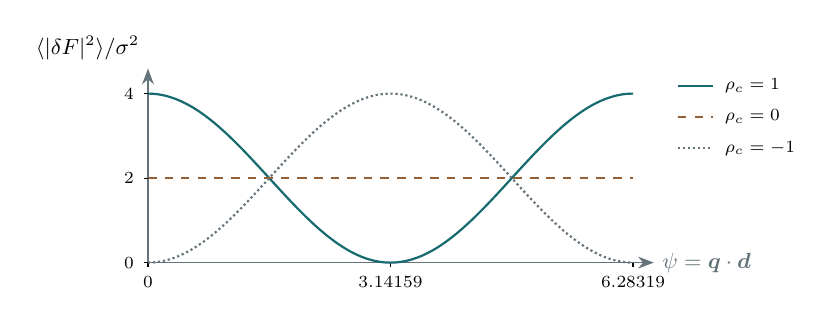
\begin{tikzpicture}[scale=.88,transform shape]
\draw[axis] (0,0.0)--(7.3,0.0) node[right] {$\psi=\boldsymbol q\cdot\boldsymbol d$};
\draw[axis] (0,0)--(0,2.8);
\node[above left] at (0,2.8) {$\langle|\delta F|^2\rangle/\sigma^2$};
\draw[thin] (0.000000,0.0)--(0.000000,-0.06);\node[below,font=\scriptsize] at (0.000000,-0.08) {$ 0 $};
\draw[thin] (3.500000,0.0)--(3.500000,-0.06);\node[below,font=\scriptsize] at (3.500000,-0.08) {$ 3.14159 $};
\draw[thin] (7.000000,0.0)--(7.000000,-0.06);\node[below,font=\scriptsize] at (7.000000,-0.08) {$ 6.28319 $};
\draw[thin] (0,0.000000)--(-.06,0.000000);\node[left,font=\scriptsize] at (-.08,0.000000) {$ 0 $};
\draw[thin] (0,1.219512)--(-.06,1.219512);\node[left,font=\scriptsize] at (-.08,1.219512) {$ 2 $};
\draw[thin] (0,2.439024)--(-.06,2.439024);\node[left,font=\scriptsize] at (-.08,2.439024) {$ 4 $};
\draw[thick,color=accent] plot coordinates {(0.0000000,2.4390244) (0.0291667,2.4386065) (0.0583333,2.4373531) (0.0875000,2.4352650) (0.1166667,2.4323438) (0.1458333,2.4285913) (0.1750000,2.4240102) (0.2041667,2.4186035) (0.2333333,2.4123751) (0.2625000,2.4053292) (0.2916667,2.3974705) (0.3208333,2.3888046) (0.3500000,2.3793372) (0.3791667,2.3690750) (0.4083333,2.3580249) (0.4375000,2.3461946) (0.4666667,2.3335920) (0.4958333,2.3202260) (0.5250000,2.3061055) (0.5541667,2.2912404) (0.5833333,2.2756407) (0.6125000,2.2593173) (0.6416667,2.2422812) (0.6708333,2.2245441) (0.7000000,2.2061183) (0.7291667,2.1870163) (0.7583333,2.1672512) (0.7875000,2.1468365) (0.8166667,2.1257864) (0.8458333,2.1041151) (0.8750000,2.0818375) (0.9041667,2.0589690) (0.9333333,2.0355251) (0.9625000,2.0115220) (0.9916667,1.9869761) (1.0208333,1.9619042) (1.0500000,1.9363235) (1.0791667,1.9102515) (1.1083333,1.8837061) (1.1375000,1.8567056) (1.1666667,1.8292683) (1.1958333,1.8014131) (1.2250000,1.7731591) (1.2541667,1.7445257) (1.2833333,1.7155325) (1.3125000,1.6861993) (1.3416667,1.6565463) (1.3708333,1.6265937) (1.4000000,1.5963622) (1.4291667,1.5658724) (1.4583333,1.5351452) (1.4875000,1.5042017) (1.5166667,1.4730630) (1.5458333,1.4417506) (1.5750000,1.4102859) (1.6041667,1.3786905) (1.6333333,1.3469859) (1.6625000,1.3151940) (1.6916667,1.2833365) (1.7208333,1.2514353) (1.7500000,1.2195122) (1.7791667,1.1875891) (1.8083333,1.1556879) (1.8375000,1.1238304) (1.8666667,1.0920385) (1.8958333,1.0603339) (1.9250000,1.0287385) (1.9541667,0.9972737) (1.9833333,0.9659614) (2.0125000,0.9348227) (2.0416667,0.9038792) (2.0708333,0.8731520) (2.1000000,0.8426622) (2.1291667,0.8124307) (2.1583333,0.7824781) (2.1875000,0.7528251) (2.2166667,0.7234919) (2.2458333,0.6944987) (2.2750000,0.6658652) (2.3041667,0.6376113) (2.3333333,0.6097561) (2.3625000,0.5823188) (2.3916667,0.5553182) (2.4208333,0.5287729) (2.4500000,0.5027009) (2.4791667,0.4771202) (2.5083333,0.4520483) (2.5375000,0.4275024) (2.5666667,0.4034993) (2.5958333,0.3800554) (2.6250000,0.3571869) (2.6541667,0.3349093) (2.6833333,0.3132380) (2.7125000,0.2921878) (2.7416667,0.2717732) (2.7708333,0.2520081) (2.8000000,0.2329061) (2.8291667,0.2144803) (2.8583333,0.1967432) (2.8875000,0.1797071) (2.9166667,0.1633837) (2.9458333,0.1477840) (2.9750000,0.1329189) (3.0041667,0.1187984) (3.0333333,0.1054324) (3.0625000,0.0928298) (3.0916667,0.0809995) (3.1208333,0.0699494) (3.1500000,0.0596872) (3.1791667,0.0502198) (3.2083333,0.0415539) (3.2375000,0.0336952) (3.2666667,0.0266493) (3.2958333,0.0204208) (3.3250000,0.0150142) (3.3541667,0.0104331) (3.3833333,0.0066806) (3.4125000,0.0037593) (3.4416667,0.0016713) (3.4708333,0.0004179) (3.5000000,0.0000000) (3.5291667,0.0004179) (3.5583333,0.0016713) (3.5875000,0.0037593) (3.6166667,0.0066806) (3.6458333,0.0104331) (3.6750000,0.0150142) (3.7041667,0.0204208) (3.7333333,0.0266493) (3.7625000,0.0336952) (3.7916667,0.0415539) (3.8208333,0.0502198) (3.8500000,0.0596872) (3.8791667,0.0699494) (3.9083333,0.0809995) (3.9375000,0.0928298) (3.9666667,0.1054324) (3.9958333,0.1187984) (4.0250000,0.1329189) (4.0541667,0.1477840) (4.0833333,0.1633837) (4.1125000,0.1797071) (4.1416667,0.1967432) (4.1708333,0.2144803) (4.2000000,0.2329061) (4.2291667,0.2520081) (4.2583333,0.2717732) (4.2875000,0.2921878) (4.3166667,0.3132380) (4.3458333,0.3349093) (4.3750000,0.3571869) (4.4041667,0.3800554) (4.4333333,0.4034993) (4.4625000,0.4275024) (4.4916667,0.4520483) (4.5208333,0.4771202) (4.5500000,0.5027009) (4.5791667,0.5287729) (4.6083333,0.5553182) (4.6375000,0.5823188) (4.6666667,0.6097561) (4.6958333,0.6376113) (4.7250000,0.6658652) (4.7541667,0.6944987) (4.7833333,0.7234919) (4.8125000,0.7528251) (4.8416667,0.7824781) (4.8708333,0.8124307) (4.9000000,0.8426622) (4.9291667,0.8731520) (4.9583333,0.9038792) (4.9875000,0.9348227) (5.0166667,0.9659614) (5.0458333,0.9972737) (5.0750000,1.0287385) (5.1041667,1.0603339) (5.1333333,1.0920385) (5.1625000,1.1238304) (5.1916667,1.1556879) (5.2208333,1.1875891) (5.2500000,1.2195122) (5.2791667,1.2514353) (5.3083333,1.2833365) (5.3375000,1.3151940) (5.3666667,1.3469859) (5.3958333,1.3786905) (5.4250000,1.4102859) (5.4541667,1.4417506) (5.4833333,1.4730630) (5.5125000,1.5042017) (5.5416667,1.5351452) (5.5708333,1.5658724) (5.6000000,1.5963622) (5.6291667,1.6265937) (5.6583333,1.6565463) (5.6875000,1.6861993) (5.7166667,1.7155325) (5.7458333,1.7445257) (5.7750000,1.7731591) (5.8041667,1.8014131) (5.8333333,1.8292683) (5.8625000,1.8567056) (5.8916667,1.8837061) (5.9208333,1.9102515) (5.9500000,1.9363235) (5.9791667,1.9619042) (6.0083333,1.9869761) (6.0375000,2.0115220) (6.0666667,2.0355251) (6.0958333,2.0589690) (6.1250000,2.0818375) (6.1541667,2.1041151) (6.1833333,2.1257864) (6.2125000,2.1468365) (6.2416667,2.1672512) (6.2708333,2.1870163) (6.3000000,2.2061183) (6.3291667,2.2245441) (6.3583333,2.2422812) (6.3875000,2.2593173) (6.4166667,2.2756407) (6.4458333,2.2912404) (6.4750000,2.3061055) (6.5041667,2.3202260) (6.5333333,2.3335920) (6.5625000,2.3461946) (6.5916667,2.3580249) (6.6208333,2.3690750) (6.6500000,2.3793372) (6.6791667,2.3888046) (6.7083333,2.3974705) (6.7375000,2.4053292) (6.7666667,2.4123751) (6.7958333,2.4186035) (6.8250000,2.4240102) (6.8541667,2.4285913) (6.8833333,2.4323438) (6.9125000,2.4352650) (6.9416667,2.4373531) (6.9708333,2.4386065) (7.0000000,2.4390244)};
\draw[thick,color=accent] (7.65,2.55)--(8.15,2.55);\node[right,font=\scriptsize] at (8.2,2.55) {$\rho_c=1$};
\draw[thick,dashed,color=warm] plot coordinates {(0.0000000,1.2195122) (0.0291667,1.2195122) (0.0583333,1.2195122) (0.0875000,1.2195122) (0.1166667,1.2195122) (0.1458333,1.2195122) (0.1750000,1.2195122) (0.2041667,1.2195122) (0.2333333,1.2195122) (0.2625000,1.2195122) (0.2916667,1.2195122) (0.3208333,1.2195122) (0.3500000,1.2195122) (0.3791667,1.2195122) (0.4083333,1.2195122) (0.4375000,1.2195122) (0.4666667,1.2195122) (0.4958333,1.2195122) (0.5250000,1.2195122) (0.5541667,1.2195122) (0.5833333,1.2195122) (0.6125000,1.2195122) (0.6416667,1.2195122) (0.6708333,1.2195122) (0.7000000,1.2195122) (0.7291667,1.2195122) (0.7583333,1.2195122) (0.7875000,1.2195122) (0.8166667,1.2195122) (0.8458333,1.2195122) (0.8750000,1.2195122) (0.9041667,1.2195122) (0.9333333,1.2195122) (0.9625000,1.2195122) (0.9916667,1.2195122) (1.0208333,1.2195122) (1.0500000,1.2195122) (1.0791667,1.2195122) (1.1083333,1.2195122) (1.1375000,1.2195122) (1.1666667,1.2195122) (1.1958333,1.2195122) (1.2250000,1.2195122) (1.2541667,1.2195122) (1.2833333,1.2195122) (1.3125000,1.2195122) (1.3416667,1.2195122) (1.3708333,1.2195122) (1.4000000,1.2195122) (1.4291667,1.2195122) (1.4583333,1.2195122) (1.4875000,1.2195122) (1.5166667,1.2195122) (1.5458333,1.2195122) (1.5750000,1.2195122) (1.6041667,1.2195122) (1.6333333,1.2195122) (1.6625000,1.2195122) (1.6916667,1.2195122) (1.7208333,1.2195122) (1.7500000,1.2195122) (1.7791667,1.2195122) (1.8083333,1.2195122) (1.8375000,1.2195122) (1.8666667,1.2195122) (1.8958333,1.2195122) (1.9250000,1.2195122) (1.9541667,1.2195122) (1.9833333,1.2195122) (2.0125000,1.2195122) (2.0416667,1.2195122) (2.0708333,1.2195122) (2.1000000,1.2195122) (2.1291667,1.2195122) (2.1583333,1.2195122) (2.1875000,1.2195122) (2.2166667,1.2195122) (2.2458333,1.2195122) (2.2750000,1.2195122) (2.3041667,1.2195122) (2.3333333,1.2195122) (2.3625000,1.2195122) (2.3916667,1.2195122) (2.4208333,1.2195122) (2.4500000,1.2195122) (2.4791667,1.2195122) (2.5083333,1.2195122) (2.5375000,1.2195122) (2.5666667,1.2195122) (2.5958333,1.2195122) (2.6250000,1.2195122) (2.6541667,1.2195122) (2.6833333,1.2195122) (2.7125000,1.2195122) (2.7416667,1.2195122) (2.7708333,1.2195122) (2.8000000,1.2195122) (2.8291667,1.2195122) (2.8583333,1.2195122) (2.8875000,1.2195122) (2.9166667,1.2195122) (2.9458333,1.2195122) (2.9750000,1.2195122) (3.0041667,1.2195122) (3.0333333,1.2195122) (3.0625000,1.2195122) (3.0916667,1.2195122) (3.1208333,1.2195122) (3.1500000,1.2195122) (3.1791667,1.2195122) (3.2083333,1.2195122) (3.2375000,1.2195122) (3.2666667,1.2195122) (3.2958333,1.2195122) (3.3250000,1.2195122) (3.3541667,1.2195122) (3.3833333,1.2195122) (3.4125000,1.2195122) (3.4416667,1.2195122) (3.4708333,1.2195122) (3.5000000,1.2195122) (3.5291667,1.2195122) (3.5583333,1.2195122) (3.5875000,1.2195122) (3.6166667,1.2195122) (3.6458333,1.2195122) (3.6750000,1.2195122) (3.7041667,1.2195122) (3.7333333,1.2195122) (3.7625000,1.2195122) (3.7916667,1.2195122) (3.8208333,1.2195122) (3.8500000,1.2195122) (3.8791667,1.2195122) (3.9083333,1.2195122) (3.9375000,1.2195122) (3.9666667,1.2195122) (3.9958333,1.2195122) (4.0250000,1.2195122) (4.0541667,1.2195122) (4.0833333,1.2195122) (4.1125000,1.2195122) (4.1416667,1.2195122) (4.1708333,1.2195122) (4.2000000,1.2195122) (4.2291667,1.2195122) (4.2583333,1.2195122) (4.2875000,1.2195122) (4.3166667,1.2195122) (4.3458333,1.2195122) (4.3750000,1.2195122) (4.4041667,1.2195122) (4.4333333,1.2195122) (4.4625000,1.2195122) (4.4916667,1.2195122) (4.5208333,1.2195122) (4.5500000,1.2195122) (4.5791667,1.2195122) (4.6083333,1.2195122) (4.6375000,1.2195122) (4.6666667,1.2195122) (4.6958333,1.2195122) (4.7250000,1.2195122) (4.7541667,1.2195122) (4.7833333,1.2195122) (4.8125000,1.2195122) (4.8416667,1.2195122) (4.8708333,1.2195122) (4.9000000,1.2195122) (4.9291667,1.2195122) (4.9583333,1.2195122) (4.9875000,1.2195122) (5.0166667,1.2195122) (5.0458333,1.2195122) (5.0750000,1.2195122) (5.1041667,1.2195122) (5.1333333,1.2195122) (5.1625000,1.2195122) (5.1916667,1.2195122) (5.2208333,1.2195122) (5.2500000,1.2195122) (5.2791667,1.2195122) (5.3083333,1.2195122) (5.3375000,1.2195122) (5.3666667,1.2195122) (5.3958333,1.2195122) (5.4250000,1.2195122) (5.4541667,1.2195122) (5.4833333,1.2195122) (5.5125000,1.2195122) (5.5416667,1.2195122) (5.5708333,1.2195122) (5.6000000,1.2195122) (5.6291667,1.2195122) (5.6583333,1.2195122) (5.6875000,1.2195122) (5.7166667,1.2195122) (5.7458333,1.2195122) (5.7750000,1.2195122) (5.8041667,1.2195122) (5.8333333,1.2195122) (5.8625000,1.2195122) (5.8916667,1.2195122) (5.9208333,1.2195122) (5.9500000,1.2195122) (5.9791667,1.2195122) (6.0083333,1.2195122) (6.0375000,1.2195122) (6.0666667,1.2195122) (6.0958333,1.2195122) (6.1250000,1.2195122) (6.1541667,1.2195122) (6.1833333,1.2195122) (6.2125000,1.2195122) (6.2416667,1.2195122) (6.2708333,1.2195122) (6.3000000,1.2195122) (6.3291667,1.2195122) (6.3583333,1.2195122) (6.3875000,1.2195122) (6.4166667,1.2195122) (6.4458333,1.2195122) (6.4750000,1.2195122) (6.5041667,1.2195122) (6.5333333,1.2195122) (6.5625000,1.2195122) (6.5916667,1.2195122) (6.6208333,1.2195122) (6.6500000,1.2195122) (6.6791667,1.2195122) (6.7083333,1.2195122) (6.7375000,1.2195122) (6.7666667,1.2195122) (6.7958333,1.2195122) (6.8250000,1.2195122) (6.8541667,1.2195122) (6.8833333,1.2195122) (6.9125000,1.2195122) (6.9416667,1.2195122) (6.9708333,1.2195122) (7.0000000,1.2195122)};
\draw[thick,dashed,color=warm] (7.65,2.0999999999999996)--(8.15,2.0999999999999996);\node[right,font=\scriptsize] at (8.2,2.0999999999999996) {$\rho_c=0$};
\draw[densely dotted,thick,color=muted] plot coordinates {(0.0000000,0.0000000) (0.0291667,0.0004179) (0.0583333,0.0016713) (0.0875000,0.0037593) (0.1166667,0.0066806) (0.1458333,0.0104331) (0.1750000,0.0150142) (0.2041667,0.0204208) (0.2333333,0.0266493) (0.2625000,0.0336952) (0.2916667,0.0415539) (0.3208333,0.0502198) (0.3500000,0.0596872) (0.3791667,0.0699494) (0.4083333,0.0809995) (0.4375000,0.0928298) (0.4666667,0.1054324) (0.4958333,0.1187984) (0.5250000,0.1329189) (0.5541667,0.1477840) (0.5833333,0.1633837) (0.6125000,0.1797071) (0.6416667,0.1967432) (0.6708333,0.2144803) (0.7000000,0.2329061) (0.7291667,0.2520081) (0.7583333,0.2717732) (0.7875000,0.2921878) (0.8166667,0.3132380) (0.8458333,0.3349093) (0.8750000,0.3571869) (0.9041667,0.3800554) (0.9333333,0.4034993) (0.9625000,0.4275024) (0.9916667,0.4520483) (1.0208333,0.4771202) (1.0500000,0.5027009) (1.0791667,0.5287729) (1.1083333,0.5553182) (1.1375000,0.5823188) (1.1666667,0.6097561) (1.1958333,0.6376113) (1.2250000,0.6658652) (1.2541667,0.6944987) (1.2833333,0.7234919) (1.3125000,0.7528251) (1.3416667,0.7824781) (1.3708333,0.8124307) (1.4000000,0.8426622) (1.4291667,0.8731520) (1.4583333,0.9038792) (1.4875000,0.9348227) (1.5166667,0.9659614) (1.5458333,0.9972737) (1.5750000,1.0287385) (1.6041667,1.0603339) (1.6333333,1.0920385) (1.6625000,1.1238304) (1.6916667,1.1556879) (1.7208333,1.1875891) (1.7500000,1.2195122) (1.7791667,1.2514353) (1.8083333,1.2833365) (1.8375000,1.3151940) (1.8666667,1.3469859) (1.8958333,1.3786905) (1.9250000,1.4102859) (1.9541667,1.4417506) (1.9833333,1.4730630) (2.0125000,1.5042017) (2.0416667,1.5351452) (2.0708333,1.5658724) (2.1000000,1.5963622) (2.1291667,1.6265937) (2.1583333,1.6565463) (2.1875000,1.6861993) (2.2166667,1.7155325) (2.2458333,1.7445257) (2.2750000,1.7731591) (2.3041667,1.8014131) (2.3333333,1.8292683) (2.3625000,1.8567056) (2.3916667,1.8837061) (2.4208333,1.9102515) (2.4500000,1.9363235) (2.4791667,1.9619042) (2.5083333,1.9869761) (2.5375000,2.0115220) (2.5666667,2.0355251) (2.5958333,2.0589690) (2.6250000,2.0818375) (2.6541667,2.1041151) (2.6833333,2.1257864) (2.7125000,2.1468365) (2.7416667,2.1672512) (2.7708333,2.1870163) (2.8000000,2.2061183) (2.8291667,2.2245441) (2.8583333,2.2422812) (2.8875000,2.2593173) (2.9166667,2.2756407) (2.9458333,2.2912404) (2.9750000,2.3061055) (3.0041667,2.3202260) (3.0333333,2.3335920) (3.0625000,2.3461946) (3.0916667,2.3580249) (3.1208333,2.3690750) (3.1500000,2.3793372) (3.1791667,2.3888046) (3.2083333,2.3974705) (3.2375000,2.4053292) (3.2666667,2.4123751) (3.2958333,2.4186035) (3.3250000,2.4240102) (3.3541667,2.4285913) (3.3833333,2.4323438) (3.4125000,2.4352650) (3.4416667,2.4373531) (3.4708333,2.4386065) (3.5000000,2.4390244) (3.5291667,2.4386065) (3.5583333,2.4373531) (3.5875000,2.4352650) (3.6166667,2.4323438) (3.6458333,2.4285913) (3.6750000,2.4240102) (3.7041667,2.4186035) (3.7333333,2.4123751) (3.7625000,2.4053292) (3.7916667,2.3974705) (3.8208333,2.3888046) (3.8500000,2.3793372) (3.8791667,2.3690750) (3.9083333,2.3580249) (3.9375000,2.3461946) (3.9666667,2.3335920) (3.9958333,2.3202260) (4.0250000,2.3061055) (4.0541667,2.2912404) (4.0833333,2.2756407) (4.1125000,2.2593173) (4.1416667,2.2422812) (4.1708333,2.2245441) (4.2000000,2.2061183) (4.2291667,2.1870163) (4.2583333,2.1672512) (4.2875000,2.1468365) (4.3166667,2.1257864) (4.3458333,2.1041151) (4.3750000,2.0818375) (4.4041667,2.0589690) (4.4333333,2.0355251) (4.4625000,2.0115220) (4.4916667,1.9869761) (4.5208333,1.9619042) (4.5500000,1.9363235) (4.5791667,1.9102515) (4.6083333,1.8837061) (4.6375000,1.8567056) (4.6666667,1.8292683) (4.6958333,1.8014131) (4.7250000,1.7731591) (4.7541667,1.7445257) (4.7833333,1.7155325) (4.8125000,1.6861993) (4.8416667,1.6565463) (4.8708333,1.6265937) (4.9000000,1.5963622) (4.9291667,1.5658724) (4.9583333,1.5351452) (4.9875000,1.5042017) (5.0166667,1.4730630) (5.0458333,1.4417506) (5.0750000,1.4102859) (5.1041667,1.3786905) (5.1333333,1.3469859) (5.1625000,1.3151940) (5.1916667,1.2833365) (5.2208333,1.2514353) (5.2500000,1.2195122) (5.2791667,1.1875891) (5.3083333,1.1556879) (5.3375000,1.1238304) (5.3666667,1.0920385) (5.3958333,1.0603339) (5.4250000,1.0287385) (5.4541667,0.9972737) (5.4833333,0.9659614) (5.5125000,0.9348227) (5.5416667,0.9038792) (5.5708333,0.8731520) (5.6000000,0.8426622) (5.6291667,0.8124307) (5.6583333,0.7824781) (5.6875000,0.7528251) (5.7166667,0.7234919) (5.7458333,0.6944987) (5.7750000,0.6658652) (5.8041667,0.6376113) (5.8333333,0.6097561) (5.8625000,0.5823188) (5.8916667,0.5553182) (5.9208333,0.5287729) (5.9500000,0.5027009) (5.9791667,0.4771202) (6.0083333,0.4520483) (6.0375000,0.4275024) (6.0666667,0.4034993) (6.0958333,0.3800554) (6.1250000,0.3571869) (6.1541667,0.3349093) (6.1833333,0.3132380) (6.2125000,0.2921878) (6.2416667,0.2717732) (6.2708333,0.2520081) (6.3000000,0.2329061) (6.3291667,0.2144803) (6.3583333,0.1967432) (6.3875000,0.1797071) (6.4166667,0.1633837) (6.4458333,0.1477840) (6.4750000,0.1329189) (6.5041667,0.1187984) (6.5333333,0.1054324) (6.5625000,0.0928298) (6.5916667,0.0809995) (6.6208333,0.0699494) (6.6500000,0.0596872) (6.6791667,0.0502198) (6.7083333,0.0415539) (6.7375000,0.0336952) (6.7666667,0.0266493) (6.7958333,0.0204208) (6.8250000,0.0150142) (6.8541667,0.0104331) (6.8833333,0.0066806) (6.9125000,0.0037593) (6.9416667,0.0016713) (6.9708333,0.0004179) (7.0000000,0.0000000)};
\draw[densely dotted,thick,color=muted] (7.65,1.65)--(8.15,1.65);\node[right,font=\scriptsize] at (8.2,1.65) {$\rho_c=-1$};
\end{tikzpicture}
\figcaption{解图光5.8C\quad 两微元的相关系数改变散射相位的角分布}
\end{minipage}\end{center}


\Needspace{13\baselineskip}

\pdfbookmark[2]{第 9 题 密度涨落的瑞利散射}{q9}

\section*{第 9 题\quad 密度涨落的瑞利散射}\label{q:9}

自然光沿$z$轴入射弱色散、光学稀薄介质。相对介电常数依赖密度$\rho$，在考察波段中$\partial\varepsilon_r/\partial\rho$可视为常量，温度对它的直接影响忽略。以远小于波长的微元作为电偶极子，由经典偶极辐射证明：短程、各向同性密度涨落造成的远场散射在角度$\theta$处满足
\[
I_\theta\propto\frac{1+\cos^2\theta}{\lambda_0^4}.
\]
给出振幅叠加、统计平均及偏振因子的推导，并说明比例式的适用条件。可用偶极远场幅度$E_s=\omega^2p\sin\alpha/(4\pi\varepsilon_0c^2r)$。

\begin{center}\begin{minipage}{.98\linewidth}\centering
\begin{tikzpicture}[scale=.9,transform shape]
\draw[axis] (-3.00000,0.00000)--(0.00000,0.00000);
\draw[axis] (0.00000,0.00000)--(3.20000,0.00000);\node[below right] at (3.20000,0.00000) {$z,\boldsymbol k_i$};\draw[axis] (0.00000,0.00000)--(0.00000,2.40000);\node[above right] at (0.00000,2.40000) {$x$};\draw[axis] (0.00000,0.00000)--(-1.30000,-1.00000);\node[below left] at (-1.30000,-1.00000) {$y$};\fill (0.00000,0.00000) circle(.035);\node[below right] at (0.00000,0.00000) {$O$};\draw[force] (0.00000,0.00000)--(2.80000,2.10000);\node[above right] at (2.80000,2.10000) {观察方向 $\boldsymbol s$};\node[above] at (1.00000,0.28000) {$\theta$};\node[above right] at (-3.00000,0.30000) {自然光};\node[below] at (1.00000,-2.00000) {散射面为 $xz$；$s$偏振垂直该面};
\end{tikzpicture}
\figcaption{图光5.9\quad 自然光两横向分量与观察方向的几何关系。}
\end{minipage}\end{center}

\Needspace{6\baselineskip}\subsection*{解答}


图光5.9以$z$为入射轴，观察方向为单位矢量$\boldsymbol s$，$\theta=\angle(\boldsymbol s,\hat{\boldsymbol z})$。把自然光分为互不相干的$x,y$两份，每份强度为总入射强度$I_0$的一半。先沿图中的$x$方向计算一份线偏振，最后加强度。

微元线度远小于波长，其内部相位近似相同，体积$v_j$的微元可看作一个电偶极子。它的偶极矩为$\boldsymbol p_j=\boldsymbol P_jv_j$，而$\boldsymbol P_j=\varepsilon_0(\varepsilon_{r,j}-1)\boldsymbol E$。写$\varepsilon_{r,j}=\bar\varepsilon_r+\delta\varepsilon_{r,j}$，均匀平均项给相干传播，涨落项在各处变化。题设忽略温度影响，对平均密度作一次展开，$\delta\varepsilon_{r,j}=(\partial\varepsilon_r/\partial\rho)\delta\rho_j$，故
\[
\delta\boldsymbol p_j=\varepsilon_0
\left(\frac{\partial\varepsilon_r}{\partial\rho}\right)
\delta\rho_j\,v_j\boldsymbol E.
\]
这里保留同一背景中的线性响应，介电密度导数在考察波段取常数。微元振幅随其体积及密度涨落共同变化。

振动偶极子的辐射远场取垂直观察方向的分量，投影算符为$Q_{\boldsymbol s}=I-\boldsymbol s\boldsymbol s^T$；$\boldsymbol s\times(\boldsymbol p\times\boldsymbol s)=Q_{\boldsymbol s}\boldsymbol p$。题给辐射式的$\sin\alpha$正是这个投影的长度。对$e^{-i\omega t}$的偶极振动，二阶时间导数给振幅中的$\omega^2$。从入射到微元、再到观察点的几何相位给$e^{-i\boldsymbol q\cdot\boldsymbol r_j}$，$\boldsymbol q=\boldsymbol k_s-\boldsymbol k_i$。去掉各项共有的传播相位后，
\[
\boldsymbol E_{s,x}
=\frac{\omega^2E_x}{4\pi c^2r}
\left(\frac{\partial\varepsilon_r}{\partial\rho}\right)
[\hat{\boldsymbol x}-(\boldsymbol s\cdot\hat{\boldsymbol x})\boldsymbol s]F_\rho(\boldsymbol q),
\]
\[
F_\rho(\boldsymbol q)=\sum_j\delta\rho_jv_j
e^{-i\boldsymbol q\cdot\boldsymbol r_j},\qquad
\boldsymbol q=\boldsymbol k_s-\boldsymbol k_i.
\]
解图光5.9A在散射面$xz$内画$x$偶极和它的观察横向投影；$y$偶极垂直纸面。具体取$\boldsymbol s=(\sin\theta,0,\cos\theta)$时，$Q_{\boldsymbol s}\hat{\boldsymbol x}=\cos\theta(\cos\theta,0,-\sin\theta)$，长度为$|\cos\theta|$，而$Q_{\boldsymbol s}\hat{\boldsymbol y}=\hat{\boldsymbol y}$，长度保持1。
\begin{center}\begin{minipage}{.98\linewidth}\centering
\begin{tikzpicture}[scale=.95,transform shape]
\draw[axis] (-1,0)--(4,0) node[right] {$z$};\draw[axis] (0,-.8)--(0,3) node[above] {$x$};
\draw[force] (0,0)--(1.7998053,2.1449244) node[above right] {$\boldsymbol s$};
\draw[motion] (0,0)--(0,2) node[left] {$\hat{\boldsymbol x}$};
\draw[force,color=warm] (0,0)--(-0.9848078,0.8263518) node[above left] {$Q_{\boldsymbol s}\hat{\boldsymbol x}$};
\draw[guide] (0,2)--(-0.9848078,0.8263518);
\node[right] at (4,.9) {$|Q_{\boldsymbol s}\hat{\boldsymbol x}|=|\cos\theta|$};
\node[right] at (4,1.8) {$Q_{\boldsymbol s}\hat{\boldsymbol y}=\hat{\boldsymbol y}$};
\node[right] at (4,2.5) {$y$垂直纸面};\node[below] at (1,.1) {$\theta$};
\end{tikzpicture}
\figcaption{解图光5.9A\quad 面内偶极的观察横向投影与面外不变分量}
\end{minipage}\end{center}
对一般方位，记$\alpha_x=\angle(\boldsymbol s,\hat{\boldsymbol x})$，投影长度的平方为$\sin^2\alpha_x$。远场与入射场在同一稀薄背景下以同一$\varepsilon_0c/2$把振幅平方转成光强；对微元涨落作平均，得
\[
\frac{I_{s,x}}{I_0/2}
=\frac{\omega^4}{16\pi^2c^4r^2}
\left(\frac{\partial\varepsilon_r}{\partial\rho}\right)^2
\langle|F_\rho(\boldsymbol q)|^2\rangle\sin^2\alpha_x.
\]
其中$F_\rho$先相干相加再取模平方，保留不同微元间的位置相位。对$y$输入有同式，仅把$\alpha_x$换成$\alpha_y$。两份输入互不相干，其散射场的平均交叉项为零，因此总光强等于两份光强之和。方向余弦满足
\[
\cos^2\alpha_x+\cos^2\alpha_y+\cos^2\theta=1,
\quad
\sin^2\alpha_x+\sin^2\alpha_y=1+\cos^2\theta.
\]
在每个观察方向，把两份强度共有的系数记为$K$，即$K=I_0\omega^4(\partial\varepsilon_r/\partial\rho)^2\langle|F_\rho(\boldsymbol q)|^2\rangle/(32\pi^2c^4r^2)$。解图光5.9B以$K$归一化，画两份贡献和总和；在$\theta=90^\circ$时，散射面内的一份沿其偶极轴观察而消失，垂直散射面的一份仍保留。由此得到
\[
I_\theta=\frac{I_0\omega^4}{32\pi^2c^4r^2}
\left(\frac{\partial\varepsilon_r}{\partial\rho}\right)^2
\langle|F_\rho(\boldsymbol q)|^2\rangle(1+\cos^2\theta).
\]
\begin{center}\begin{minipage}{.98\linewidth}\centering
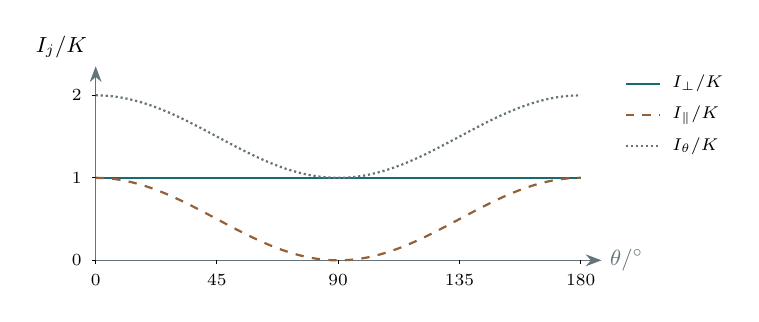
\begin{tikzpicture}[scale=.88,transform shape]
\draw[axis] (0,0.0)--(7.3,0.0) node[right] {$\theta/{}^\circ$};
\draw[axis] (0,0)--(0,2.8);
\node[above left] at (0,2.8) {$I_j/K$};
\draw[thin] (0.000000,0.0)--(0.000000,-0.06);\node[below,font=\scriptsize] at (0.000000,-0.08) {$ 0 $};
\draw[thin] (1.750000,0.0)--(1.750000,-0.06);\node[below,font=\scriptsize] at (1.750000,-0.08) {$ 45 $};
\draw[thin] (3.500000,0.0)--(3.500000,-0.06);\node[below,font=\scriptsize] at (3.500000,-0.08) {$ 90 $};
\draw[thin] (5.250000,0.0)--(5.250000,-0.06);\node[below,font=\scriptsize] at (5.250000,-0.08) {$ 135 $};
\draw[thin] (7.000000,0.0)--(7.000000,-0.06);\node[below,font=\scriptsize] at (7.000000,-0.08) {$ 180 $};
\draw[thin] (0,0.000000)--(-.06,0.000000);\node[left,font=\scriptsize] at (-.08,0.000000) {$ 0 $};
\draw[thin] (0,1.190476)--(-.06,1.190476);\node[left,font=\scriptsize] at (-.08,1.190476) {$ 1 $};
\draw[thin] (0,2.380952)--(-.06,2.380952);\node[left,font=\scriptsize] at (-.08,2.380952) {$ 2 $};
\draw[thick,color=accent] plot coordinates {(0.0000000,1.1904762) (0.0291667,1.1904762) (0.0583333,1.1904762) (0.0875000,1.1904762) (0.1166667,1.1904762) (0.1458333,1.1904762) (0.1750000,1.1904762) (0.2041667,1.1904762) (0.2333333,1.1904762) (0.2625000,1.1904762) (0.2916667,1.1904762) (0.3208333,1.1904762) (0.3500000,1.1904762) (0.3791667,1.1904762) (0.4083333,1.1904762) (0.4375000,1.1904762) (0.4666667,1.1904762) (0.4958333,1.1904762) (0.5250000,1.1904762) (0.5541667,1.1904762) (0.5833333,1.1904762) (0.6125000,1.1904762) (0.6416667,1.1904762) (0.6708333,1.1904762) (0.7000000,1.1904762) (0.7291667,1.1904762) (0.7583333,1.1904762) (0.7875000,1.1904762) (0.8166667,1.1904762) (0.8458333,1.1904762) (0.8750000,1.1904762) (0.9041667,1.1904762) (0.9333333,1.1904762) (0.9625000,1.1904762) (0.9916667,1.1904762) (1.0208333,1.1904762) (1.0500000,1.1904762) (1.0791667,1.1904762) (1.1083333,1.1904762) (1.1375000,1.1904762) (1.1666667,1.1904762) (1.1958333,1.1904762) (1.2250000,1.1904762) (1.2541667,1.1904762) (1.2833333,1.1904762) (1.3125000,1.1904762) (1.3416667,1.1904762) (1.3708333,1.1904762) (1.4000000,1.1904762) (1.4291667,1.1904762) (1.4583333,1.1904762) (1.4875000,1.1904762) (1.5166667,1.1904762) (1.5458333,1.1904762) (1.5750000,1.1904762) (1.6041667,1.1904762) (1.6333333,1.1904762) (1.6625000,1.1904762) (1.6916667,1.1904762) (1.7208333,1.1904762) (1.7500000,1.1904762) (1.7791667,1.1904762) (1.8083333,1.1904762) (1.8375000,1.1904762) (1.8666667,1.1904762) (1.8958333,1.1904762) (1.9250000,1.1904762) (1.9541667,1.1904762) (1.9833333,1.1904762) (2.0125000,1.1904762) (2.0416667,1.1904762) (2.0708333,1.1904762) (2.1000000,1.1904762) (2.1291667,1.1904762) (2.1583333,1.1904762) (2.1875000,1.1904762) (2.2166667,1.1904762) (2.2458333,1.1904762) (2.2750000,1.1904762) (2.3041667,1.1904762) (2.3333333,1.1904762) (2.3625000,1.1904762) (2.3916667,1.1904762) (2.4208333,1.1904762) (2.4500000,1.1904762) (2.4791667,1.1904762) (2.5083333,1.1904762) (2.5375000,1.1904762) (2.5666667,1.1904762) (2.5958333,1.1904762) (2.6250000,1.1904762) (2.6541667,1.1904762) (2.6833333,1.1904762) (2.7125000,1.1904762) (2.7416667,1.1904762) (2.7708333,1.1904762) (2.8000000,1.1904762) (2.8291667,1.1904762) (2.8583333,1.1904762) (2.8875000,1.1904762) (2.9166667,1.1904762) (2.9458333,1.1904762) (2.9750000,1.1904762) (3.0041667,1.1904762) (3.0333333,1.1904762) (3.0625000,1.1904762) (3.0916667,1.1904762) (3.1208333,1.1904762) (3.1500000,1.1904762) (3.1791667,1.1904762) (3.2083333,1.1904762) (3.2375000,1.1904762) (3.2666667,1.1904762) (3.2958333,1.1904762) (3.3250000,1.1904762) (3.3541667,1.1904762) (3.3833333,1.1904762) (3.4125000,1.1904762) (3.4416667,1.1904762) (3.4708333,1.1904762) (3.5000000,1.1904762) (3.5291667,1.1904762) (3.5583333,1.1904762) (3.5875000,1.1904762) (3.6166667,1.1904762) (3.6458333,1.1904762) (3.6750000,1.1904762) (3.7041667,1.1904762) (3.7333333,1.1904762) (3.7625000,1.1904762) (3.7916667,1.1904762) (3.8208333,1.1904762) (3.8500000,1.1904762) (3.8791667,1.1904762) (3.9083333,1.1904762) (3.9375000,1.1904762) (3.9666667,1.1904762) (3.9958333,1.1904762) (4.0250000,1.1904762) (4.0541667,1.1904762) (4.0833333,1.1904762) (4.1125000,1.1904762) (4.1416667,1.1904762) (4.1708333,1.1904762) (4.2000000,1.1904762) (4.2291667,1.1904762) (4.2583333,1.1904762) (4.2875000,1.1904762) (4.3166667,1.1904762) (4.3458333,1.1904762) (4.3750000,1.1904762) (4.4041667,1.1904762) (4.4333333,1.1904762) (4.4625000,1.1904762) (4.4916667,1.1904762) (4.5208333,1.1904762) (4.5500000,1.1904762) (4.5791667,1.1904762) (4.6083333,1.1904762) (4.6375000,1.1904762) (4.6666667,1.1904762) (4.6958333,1.1904762) (4.7250000,1.1904762) (4.7541667,1.1904762) (4.7833333,1.1904762) (4.8125000,1.1904762) (4.8416667,1.1904762) (4.8708333,1.1904762) (4.9000000,1.1904762) (4.9291667,1.1904762) (4.9583333,1.1904762) (4.9875000,1.1904762) (5.0166667,1.1904762) (5.0458333,1.1904762) (5.0750000,1.1904762) (5.1041667,1.1904762) (5.1333333,1.1904762) (5.1625000,1.1904762) (5.1916667,1.1904762) (5.2208333,1.1904762) (5.2500000,1.1904762) (5.2791667,1.1904762) (5.3083333,1.1904762) (5.3375000,1.1904762) (5.3666667,1.1904762) (5.3958333,1.1904762) (5.4250000,1.1904762) (5.4541667,1.1904762) (5.4833333,1.1904762) (5.5125000,1.1904762) (5.5416667,1.1904762) (5.5708333,1.1904762) (5.6000000,1.1904762) (5.6291667,1.1904762) (5.6583333,1.1904762) (5.6875000,1.1904762) (5.7166667,1.1904762) (5.7458333,1.1904762) (5.7750000,1.1904762) (5.8041667,1.1904762) (5.8333333,1.1904762) (5.8625000,1.1904762) (5.8916667,1.1904762) (5.9208333,1.1904762) (5.9500000,1.1904762) (5.9791667,1.1904762) (6.0083333,1.1904762) (6.0375000,1.1904762) (6.0666667,1.1904762) (6.0958333,1.1904762) (6.1250000,1.1904762) (6.1541667,1.1904762) (6.1833333,1.1904762) (6.2125000,1.1904762) (6.2416667,1.1904762) (6.2708333,1.1904762) (6.3000000,1.1904762) (6.3291667,1.1904762) (6.3583333,1.1904762) (6.3875000,1.1904762) (6.4166667,1.1904762) (6.4458333,1.1904762) (6.4750000,1.1904762) (6.5041667,1.1904762) (6.5333333,1.1904762) (6.5625000,1.1904762) (6.5916667,1.1904762) (6.6208333,1.1904762) (6.6500000,1.1904762) (6.6791667,1.1904762) (6.7083333,1.1904762) (6.7375000,1.1904762) (6.7666667,1.1904762) (6.7958333,1.1904762) (6.8250000,1.1904762) (6.8541667,1.1904762) (6.8833333,1.1904762) (6.9125000,1.1904762) (6.9416667,1.1904762) (6.9708333,1.1904762) (7.0000000,1.1904762)};
\draw[thick,color=accent] (7.65,2.55)--(8.15,2.55);\node[right,font=\scriptsize] at (8.2,2.55) {$I_\perp/K$};
\draw[thick,dashed,color=warm] plot coordinates {(0.0000000,1.1904762) (0.0291667,1.1902722) (0.0583333,1.1896604) (0.0875000,1.1886413) (0.1166667,1.1872154) (0.1458333,1.1853838) (0.1750000,1.1831478) (0.2041667,1.1805089) (0.2333333,1.1774688) (0.2625000,1.1740297) (0.2916667,1.1701939) (0.3208333,1.1659641) (0.3500000,1.1613432) (0.3791667,1.1563342) (0.4083333,1.1509407) (0.4375000,1.1451664) (0.4666667,1.1390152) (0.4958333,1.1324912) (0.5250000,1.1255991) (0.5541667,1.1183435) (0.5833333,1.1107294) (0.6125000,1.1027620) (0.6416667,1.0944468) (0.6708333,1.0857894) (0.7000000,1.0767958) (0.7291667,1.0674722) (0.7583333,1.0578250) (0.7875000,1.0478607) (0.8166667,1.0375862) (0.8458333,1.0270086) (0.8750000,1.0161350) (0.9041667,1.0049730) (0.9333333,0.9935301) (0.9625000,0.9818143) (0.9916667,0.9698336) (1.0208333,0.9575961) (1.0500000,0.9451103) (1.0791667,0.9323847) (1.1083333,0.9194280) (1.1375000,0.9062491) (1.1666667,0.8928571) (1.1958333,0.8792612) (1.2250000,0.8654705) (1.2541667,0.8514947) (1.2833333,0.8373432) (1.3125000,0.8230259) (1.3416667,0.8085524) (1.3708333,0.7939327) (1.4000000,0.7791768) (1.4291667,0.7642948) (1.4583333,0.7492971) (1.4875000,0.7341937) (1.5166667,0.7189951) (1.5458333,0.7037116) (1.5750000,0.6883538) (1.6041667,0.6729323) (1.6333333,0.6574574) (1.6625000,0.6419399) (1.6916667,0.6263905) (1.7208333,0.6108196) (1.7500000,0.5952381) (1.7791667,0.5796566) (1.8083333,0.5640857) (1.8375000,0.5485363) (1.8666667,0.5330188) (1.8958333,0.5175439) (1.9250000,0.5021223) (1.9541667,0.4867646) (1.9833333,0.4714811) (2.0125000,0.4562825) (2.0416667,0.4411791) (2.0708333,0.4261813) (2.1000000,0.4112994) (2.1291667,0.3965435) (2.1583333,0.3819238) (2.1875000,0.3674503) (2.2166667,0.3531330) (2.2458333,0.3389815) (2.2750000,0.3250057) (2.3041667,0.3112150) (2.3333333,0.2976190) (2.3625000,0.2842270) (2.3916667,0.2710482) (2.4208333,0.2580915) (2.4500000,0.2453659) (2.4791667,0.2328801) (2.5083333,0.2206426) (2.5375000,0.2086619) (2.5666667,0.1969461) (2.5958333,0.1855032) (2.6250000,0.1743412) (2.6541667,0.1634676) (2.6833333,0.1528900) (2.7125000,0.1426155) (2.7416667,0.1326512) (2.7708333,0.1230040) (2.8000000,0.1136804) (2.8291667,0.1046868) (2.8583333,0.0960294) (2.8875000,0.0877142) (2.9166667,0.0797468) (2.9458333,0.0721327) (2.9750000,0.0648771) (3.0041667,0.0579849) (3.0333333,0.0514610) (3.0625000,0.0453098) (3.0916667,0.0395355) (3.1208333,0.0341420) (3.1500000,0.0291330) (3.1791667,0.0245121) (3.2083333,0.0202822) (3.2375000,0.0164465) (3.2666667,0.0130074) (3.2958333,0.0099673) (3.3250000,0.0073284) (3.3541667,0.0050923) (3.3833333,0.0032608) (3.4125000,0.0018349) (3.4416667,0.0008158) (3.4708333,0.0002040) (3.5000000,0.0000000) (3.5291667,0.0002040) (3.5583333,0.0008158) (3.5875000,0.0018349) (3.6166667,0.0032608) (3.6458333,0.0050923) (3.6750000,0.0073284) (3.7041667,0.0099673) (3.7333333,0.0130074) (3.7625000,0.0164465) (3.7916667,0.0202822) (3.8208333,0.0245121) (3.8500000,0.0291330) (3.8791667,0.0341420) (3.9083333,0.0395355) (3.9375000,0.0453098) (3.9666667,0.0514610) (3.9958333,0.0579849) (4.0250000,0.0648771) (4.0541667,0.0721327) (4.0833333,0.0797468) (4.1125000,0.0877142) (4.1416667,0.0960294) (4.1708333,0.1046868) (4.2000000,0.1136804) (4.2291667,0.1230040) (4.2583333,0.1326512) (4.2875000,0.1426155) (4.3166667,0.1528900) (4.3458333,0.1634676) (4.3750000,0.1743412) (4.4041667,0.1855032) (4.4333333,0.1969461) (4.4625000,0.2086619) (4.4916667,0.2206426) (4.5208333,0.2328801) (4.5500000,0.2453659) (4.5791667,0.2580915) (4.6083333,0.2710482) (4.6375000,0.2842270) (4.6666667,0.2976190) (4.6958333,0.3112150) (4.7250000,0.3250057) (4.7541667,0.3389815) (4.7833333,0.3531330) (4.8125000,0.3674503) (4.8416667,0.3819238) (4.8708333,0.3965435) (4.9000000,0.4112994) (4.9291667,0.4261813) (4.9583333,0.4411791) (4.9875000,0.4562825) (5.0166667,0.4714811) (5.0458333,0.4867646) (5.0750000,0.5021223) (5.1041667,0.5175439) (5.1333333,0.5330188) (5.1625000,0.5485363) (5.1916667,0.5640857) (5.2208333,0.5796566) (5.2500000,0.5952381) (5.2791667,0.6108196) (5.3083333,0.6263905) (5.3375000,0.6419399) (5.3666667,0.6574574) (5.3958333,0.6729323) (5.4250000,0.6883538) (5.4541667,0.7037116) (5.4833333,0.7189951) (5.5125000,0.7341937) (5.5416667,0.7492971) (5.5708333,0.7642948) (5.6000000,0.7791768) (5.6291667,0.7939327) (5.6583333,0.8085524) (5.6875000,0.8230259) (5.7166667,0.8373432) (5.7458333,0.8514947) (5.7750000,0.8654705) (5.8041667,0.8792612) (5.8333333,0.8928571) (5.8625000,0.9062491) (5.8916667,0.9194280) (5.9208333,0.9323847) (5.9500000,0.9451103) (5.9791667,0.9575961) (6.0083333,0.9698336) (6.0375000,0.9818143) (6.0666667,0.9935301) (6.0958333,1.0049730) (6.1250000,1.0161350) (6.1541667,1.0270086) (6.1833333,1.0375862) (6.2125000,1.0478607) (6.2416667,1.0578250) (6.2708333,1.0674722) (6.3000000,1.0767958) (6.3291667,1.0857894) (6.3583333,1.0944468) (6.3875000,1.1027620) (6.4166667,1.1107294) (6.4458333,1.1183435) (6.4750000,1.1255991) (6.5041667,1.1324912) (6.5333333,1.1390152) (6.5625000,1.1451664) (6.5916667,1.1509407) (6.6208333,1.1563342) (6.6500000,1.1613432) (6.6791667,1.1659641) (6.7083333,1.1701939) (6.7375000,1.1740297) (6.7666667,1.1774688) (6.7958333,1.1805089) (6.8250000,1.1831478) (6.8541667,1.1853838) (6.8833333,1.1872154) (6.9125000,1.1886413) (6.9416667,1.1896604) (6.9708333,1.1902722) (7.0000000,1.1904762)};
\draw[thick,dashed,color=warm] (7.65,2.0999999999999996)--(8.15,2.0999999999999996);\node[right,font=\scriptsize] at (8.2,2.0999999999999996) {$I_\parallel/K$};
\draw[densely dotted,thick,color=muted] plot coordinates {(0.0000000,2.3809524) (0.0291667,2.3807484) (0.0583333,2.3801366) (0.0875000,2.3791175) (0.1166667,2.3776916) (0.1458333,2.3758600) (0.1750000,2.3736240) (0.2041667,2.3709851) (0.2333333,2.3679450) (0.2625000,2.3645059) (0.2916667,2.3606701) (0.3208333,2.3564403) (0.3500000,2.3518194) (0.3791667,2.3468104) (0.4083333,2.3414169) (0.4375000,2.3356426) (0.4666667,2.3294913) (0.4958333,2.3229674) (0.5250000,2.3160753) (0.5541667,2.3088197) (0.5833333,2.3012056) (0.6125000,2.2932382) (0.6416667,2.2849230) (0.6708333,2.2762656) (0.7000000,2.2672720) (0.7291667,2.2579484) (0.7583333,2.2483012) (0.7875000,2.2383369) (0.8166667,2.2280624) (0.8458333,2.2174847) (0.8750000,2.2066112) (0.9041667,2.1954492) (0.9333333,2.1840063) (0.9625000,2.1722905) (0.9916667,2.1603098) (1.0208333,2.1480723) (1.0500000,2.1355865) (1.0791667,2.1228609) (1.1083333,2.1099042) (1.1375000,2.0967253) (1.1666667,2.0833333) (1.1958333,2.0697374) (1.2250000,2.0559467) (1.2541667,2.0419709) (1.2833333,2.0278194) (1.3125000,2.0135020) (1.3416667,1.9990285) (1.3708333,1.9844088) (1.4000000,1.9696530) (1.4291667,1.9547710) (1.4583333,1.9397732) (1.4875000,1.9246699) (1.5166667,1.9094712) (1.5458333,1.8941878) (1.5750000,1.8788300) (1.6041667,1.8634084) (1.6333333,1.8479336) (1.6625000,1.8324161) (1.6916667,1.8168666) (1.7208333,1.8012958) (1.7500000,1.7857143) (1.7791667,1.7701328) (1.8083333,1.7545619) (1.8375000,1.7390124) (1.8666667,1.7234950) (1.8958333,1.7080201) (1.9250000,1.6925985) (1.9541667,1.6772408) (1.9833333,1.6619573) (2.0125000,1.6467587) (2.0416667,1.6316553) (2.0708333,1.6166575) (2.1000000,1.6017756) (2.1291667,1.5870197) (2.1583333,1.5724000) (2.1875000,1.5579265) (2.2166667,1.5436091) (2.2458333,1.5294577) (2.2750000,1.5154818) (2.3041667,1.5016912) (2.3333333,1.4880952) (2.3625000,1.4747032) (2.3916667,1.4615244) (2.4208333,1.4485677) (2.4500000,1.4358421) (2.4791667,1.4233563) (2.5083333,1.4111188) (2.5375000,1.3991381) (2.5666667,1.3874223) (2.5958333,1.3759794) (2.6250000,1.3648174) (2.6541667,1.3539438) (2.6833333,1.3433662) (2.7125000,1.3330917) (2.7416667,1.3231274) (2.7708333,1.3134802) (2.8000000,1.3041566) (2.8291667,1.2951630) (2.8583333,1.2865056) (2.8875000,1.2781904) (2.9166667,1.2702230) (2.9458333,1.2626089) (2.9750000,1.2553533) (3.0041667,1.2484611) (3.0333333,1.2419372) (3.0625000,1.2357860) (3.0916667,1.2300117) (3.1208333,1.2246182) (3.1500000,1.2196092) (3.1791667,1.2149883) (3.2083333,1.2107584) (3.2375000,1.2069227) (3.2666667,1.2034836) (3.2958333,1.2004435) (3.3250000,1.1978046) (3.3541667,1.1955685) (3.3833333,1.1937370) (3.4125000,1.1923111) (3.4416667,1.1912919) (3.4708333,1.1906802) (3.5000000,1.1904762) (3.5291667,1.1906802) (3.5583333,1.1912919) (3.5875000,1.1923111) (3.6166667,1.1937370) (3.6458333,1.1955685) (3.6750000,1.1978046) (3.7041667,1.2004435) (3.7333333,1.2034836) (3.7625000,1.2069227) (3.7916667,1.2107584) (3.8208333,1.2149883) (3.8500000,1.2196092) (3.8791667,1.2246182) (3.9083333,1.2300117) (3.9375000,1.2357860) (3.9666667,1.2419372) (3.9958333,1.2484611) (4.0250000,1.2553533) (4.0541667,1.2626089) (4.0833333,1.2702230) (4.1125000,1.2781904) (4.1416667,1.2865056) (4.1708333,1.2951630) (4.2000000,1.3041566) (4.2291667,1.3134802) (4.2583333,1.3231274) (4.2875000,1.3330917) (4.3166667,1.3433662) (4.3458333,1.3539438) (4.3750000,1.3648174) (4.4041667,1.3759794) (4.4333333,1.3874223) (4.4625000,1.3991381) (4.4916667,1.4111188) (4.5208333,1.4233563) (4.5500000,1.4358421) (4.5791667,1.4485677) (4.6083333,1.4615244) (4.6375000,1.4747032) (4.6666667,1.4880952) (4.6958333,1.5016912) (4.7250000,1.5154818) (4.7541667,1.5294577) (4.7833333,1.5436091) (4.8125000,1.5579265) (4.8416667,1.5724000) (4.8708333,1.5870197) (4.9000000,1.6017756) (4.9291667,1.6166575) (4.9583333,1.6316553) (4.9875000,1.6467587) (5.0166667,1.6619573) (5.0458333,1.6772408) (5.0750000,1.6925985) (5.1041667,1.7080201) (5.1333333,1.7234950) (5.1625000,1.7390124) (5.1916667,1.7545619) (5.2208333,1.7701328) (5.2500000,1.7857143) (5.2791667,1.8012958) (5.3083333,1.8168666) (5.3375000,1.8324161) (5.3666667,1.8479336) (5.3958333,1.8634084) (5.4250000,1.8788300) (5.4541667,1.8941878) (5.4833333,1.9094712) (5.5125000,1.9246699) (5.5416667,1.9397732) (5.5708333,1.9547710) (5.6000000,1.9696530) (5.6291667,1.9844088) (5.6583333,1.9990285) (5.6875000,2.0135020) (5.7166667,2.0278194) (5.7458333,2.0419709) (5.7750000,2.0559467) (5.8041667,2.0697374) (5.8333333,2.0833333) (5.8625000,2.0967253) (5.8916667,2.1099042) (5.9208333,2.1228609) (5.9500000,2.1355865) (5.9791667,2.1480723) (6.0083333,2.1603098) (6.0375000,2.1722905) (6.0666667,2.1840063) (6.0958333,2.1954492) (6.1250000,2.2066112) (6.1541667,2.2174847) (6.1833333,2.2280624) (6.2125000,2.2383369) (6.2416667,2.2483012) (6.2708333,2.2579484) (6.3000000,2.2672720) (6.3291667,2.2762656) (6.3583333,2.2849230) (6.3875000,2.2932382) (6.4166667,2.3012056) (6.4458333,2.3088197) (6.4750000,2.3160753) (6.5041667,2.3229674) (6.5333333,2.3294913) (6.5625000,2.3356426) (6.5916667,2.3414169) (6.6208333,2.3468104) (6.6500000,2.3518194) (6.6791667,2.3564403) (6.7083333,2.3606701) (6.7375000,2.3645059) (6.7666667,2.3679450) (6.7958333,2.3709851) (6.8250000,2.3736240) (6.8541667,2.3758600) (6.8833333,2.3776916) (6.9125000,2.3791175) (6.9416667,2.3801366) (6.9708333,2.3807484) (7.0000000,2.3809524)};
\draw[densely dotted,thick,color=muted] (7.65,1.65)--(8.15,1.65);\node[right,font=\scriptsize] at (8.2,1.65) {$I_\theta/K$};
\end{tikzpicture}
\figcaption{解图光5.9B\quad 自然光两份输出与相加后的瑞利角因子}
\end{minipage}\end{center}
固定观察距离后，把$\omega=2\pi c/\lambda_0$代入，辐射强度中的$\omega^4/c^4$化为$(2\pi)^4/\lambda_0^4$。这个显式的负四次方还乘以密度的相关谱。连续介质中记$C_\rho(\boldsymbol R)=\langle\delta\rho(\boldsymbol r)\delta\rho(\boldsymbol r+\boldsymbol R)\rangle$，双重和成为
\[
\langle|F_\rho|^2\rangle
=\int_V\!\int_V C_\rho(\boldsymbol r-\boldsymbol r')
e^{-i\boldsymbol q\cdot(\boldsymbol r-\boldsymbol r')}\dd^3r\,\dd^3r'
\simeq V\widetilde C_\rho(\boldsymbol q).
\]
最后一步使用统计均匀性，且样品尺寸远大于密度相关长度$\xi$，使相对坐标积分近似延伸至全空间，中心坐标积分给体积$V$。散射矢量大小在稀薄背景中为$q=2k\sin(\theta/2)$；若全部考察角度满足$q\xi\ll1$，则Fourier核在主要相关距离内近于1，$\widetilde C_\rho(\boldsymbol q)\simeq\widetilde C_\rho(0)$。背景折射率和介电密度导数在波段内变化缓慢，并处于单次散射近似时，
\[
\boxed{I_\theta\propto(1+\cos^2\theta)/\lambda_0^4}.
\]
解图光5.9C用固定角度下的波长曲线展示这一规律，450nm与650nm的比值约为4.35。它由偶极辐射的时间导数和短程密度相关共同给出。若相关长度增大，完整式中的$\widetilde C_\rho(\boldsymbol q)$保留角度与波长依赖；解图光5.9D取$\widetilde C_\rho(q)/\widetilde C_\rho(0)=e^{-q^2\xi^2/2}$，每条曲线以相应的前向散射强度$I_0^{\rm sc}=I_{\theta=0}$归一化，因此
\[
 \frac{I_\theta}{I_0^{\rm sc}}=\frac{1+\cos^2\theta}{2}\exp[-2k^2\xi^2\sin^2(\theta/2)].
\]
由此可见大角散射受到额外抑制。上述计算使用线度远小于波长的微元、稀薄背景远场和单次散射；短程条件再将密度相关谱取作常数，得到题设的瑞利角分布与波长关系。
\begin{center}\begin{minipage}{.98\linewidth}\centering
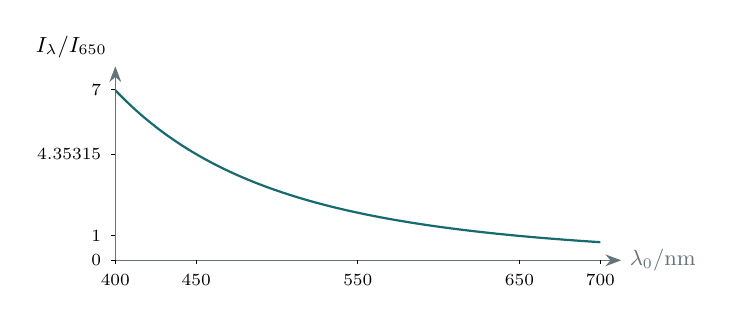
\begin{tikzpicture}[scale=.88,transform shape]
\draw[axis] (0,0.0)--(7.3,0.0) node[right] {$\lambda_0/\mathrm{nm}$};
\draw[axis] (0,0)--(0,2.8);
\node[above left] at (0,2.8) {$I_\lambda/I_{650}$};
\draw[thin] (0.000000,0.0)--(0.000000,-0.06);\node[below,font=\scriptsize] at (0.000000,-0.08) {$ 400 $};
\draw[thin] (1.166667,0.0)--(1.166667,-0.06);\node[below,font=\scriptsize] at (1.166667,-0.08) {$ 450 $};
\draw[thin] (3.500000,0.0)--(3.500000,-0.06);\node[below,font=\scriptsize] at (3.500000,-0.08) {$ 550 $};
\draw[thin] (5.833333,0.0)--(5.833333,-0.06);\node[below,font=\scriptsize] at (5.833333,-0.08) {$ 650 $};
\draw[thin] (7.000000,0.0)--(7.000000,-0.06);\node[below,font=\scriptsize] at (7.000000,-0.08) {$ 700 $};
\draw[thin] (0,0.000000)--(-.06,0.000000);\node[left,font=\scriptsize] at (-.08,0.000000) {$ 0 $};
\draw[thin] (0,0.352113)--(-.06,0.352113);\node[left,font=\scriptsize] at (-.08,0.352113) {$ 1 $};
\draw[thin] (0,1.532799)--(-.06,1.532799);\node[left,font=\scriptsize] at (-.08,1.532799) {$ 4.35315 $};
\draw[thin] (0,2.464789)--(-.06,2.464789);\node[left,font=\scriptsize] at (-.08,2.464789) {$ 7 $};
\draw[thick,color=accent] plot coordinates {(0.0000000,2.4552466) (0.0291667,2.4247943) (0.0583333,2.3948127) (0.0875000,2.3652930) (0.1166667,2.3362268) (0.1458333,2.3076056) (0.1750000,2.2794215) (0.2041667,2.2516663) (0.2333333,2.2243323) (0.2625000,2.1974118) (0.2916667,2.1708973) (0.3208333,2.1447815) (0.3500000,2.1190573) (0.3791667,2.0937176) (0.4083333,2.0687555) (0.4375000,2.0441643) (0.4666667,2.0199375) (0.4958333,1.9960685) (0.5250000,1.9725510) (0.5541667,1.9493788) (0.5833333,1.9265459) (0.6125000,1.9040464) (0.6416667,1.8818743) (0.6708333,1.8600240) (0.7000000,1.8384900) (0.7291667,1.8172666) (0.7583333,1.7963487) (0.7875000,1.7757308) (0.8166667,1.7554079) (0.8458333,1.7353750) (0.8750000,1.7156269) (0.9041667,1.6961590) (0.9333333,1.6769665) (0.9625000,1.6580446) (0.9916667,1.6393889) (1.0208333,1.6209948) (1.0500000,1.6028580) (1.0791667,1.5849741) (1.1083333,1.5673390) (1.1375000,1.5499484) (1.1666667,1.5327984) (1.1958333,1.5158849) (1.2250000,1.4992041) (1.2541667,1.4827521) (1.2833333,1.4665251) (1.3125000,1.4505195) (1.3416667,1.4347317) (1.3708333,1.4191581) (1.4000000,1.4037952) (1.4291667,1.3886397) (1.4583333,1.3736881) (1.4875000,1.3589372) (1.5166667,1.3443838) (1.5458333,1.3300247) (1.5750000,1.3158568) (1.6041667,1.3018770) (1.6333333,1.2880824) (1.6625000,1.2744700) (1.6916667,1.2610370) (1.7208333,1.2477805) (1.7500000,1.2346977) (1.7791667,1.2217860) (1.8083333,1.2090425) (1.8375000,1.1964648) (1.8666667,1.1840503) (1.8958333,1.1717963) (1.9250000,1.1597004) (1.9541667,1.1477602) (1.9833333,1.1359733) (2.0125000,1.1243373) (2.0416667,1.1128499) (2.0708333,1.1015089) (2.1000000,1.0903119) (2.1291667,1.0792569) (2.1583333,1.0683416) (2.1875000,1.0575640) (2.2166667,1.0469219) (2.2458333,1.0364134) (2.2750000,1.0260363) (2.3041667,1.0157889) (2.3333333,1.0056690) (2.3625000,0.9956749) (2.3916667,0.9858046) (2.4208333,0.9760563) (2.4500000,0.9664282) (2.4791667,0.9569185) (2.5083333,0.9475255) (2.5375000,0.9382475) (2.5666667,0.9290827) (2.5958333,0.9200296) (2.6250000,0.9110865) (2.6541667,0.9022518) (2.6833333,0.8935239) (2.7125000,0.8849013) (2.7416667,0.8763824) (2.7708333,0.8679659) (2.8000000,0.8596501) (2.8291667,0.8514337) (2.8583333,0.8433152) (2.8875000,0.8352932) (2.9166667,0.8273664) (2.9458333,0.8195334) (2.9750000,0.8117929) (3.0041667,0.8041435) (3.0333333,0.7965841) (3.0625000,0.7891132) (3.0916667,0.7817297) (3.1208333,0.7744324) (3.1500000,0.7672201) (3.1791667,0.7600915) (3.2083333,0.7530455) (3.2375000,0.7460810) (3.2666667,0.7391967) (3.2958333,0.7323918) (3.3250000,0.7256649) (3.3541667,0.7190151) (3.3833333,0.7124413) (3.4125000,0.7059424) (3.4416667,0.6995175) (3.4708333,0.6931655) (3.5000000,0.6868855) (3.5291667,0.6806764) (3.5583333,0.6745373) (3.5875000,0.6684672) (3.6166667,0.6624653) (3.6458333,0.6565306) (3.6750000,0.6506622) (3.7041667,0.6448593) (3.7333333,0.6391208) (3.7625000,0.6334461) (3.7916667,0.6278342) (3.8208333,0.6222843) (3.8500000,0.6167956) (3.8791667,0.6113673) (3.9083333,0.6059986) (3.9375000,0.6006887) (3.9666667,0.5954368) (3.9958333,0.5902422) (4.0250000,0.5851041) (4.0541667,0.5800218) (4.0833333,0.5749945) (4.1125000,0.5700216) (4.1416667,0.5651024) (4.1708333,0.5602361) (4.2000000,0.5554220) (4.2291667,0.5506596) (4.2583333,0.5459481) (4.2875000,0.5412869) (4.3166667,0.5366753) (4.3458333,0.5321127) (4.3750000,0.5275986) (4.4041667,0.5231321) (4.4333333,0.5187129) (4.4625000,0.5143402) (4.4916667,0.5100135) (4.5208333,0.5057322) (4.5500000,0.5014957) (4.5791667,0.4973035) (4.6083333,0.4931550) (4.6375000,0.4890497) (4.6666667,0.4849870) (4.6958333,0.4809664) (4.7250000,0.4769874) (4.7541667,0.4730494) (4.7833333,0.4691520) (4.8125000,0.4652947) (4.8416667,0.4614769) (4.8708333,0.4576982) (4.9000000,0.4539581) (4.9291667,0.4502561) (4.9583333,0.4465918) (4.9875000,0.4429646) (5.0166667,0.4393743) (5.0458333,0.4358202) (5.0750000,0.4323020) (5.1041667,0.4288192) (5.1333333,0.4253714) (5.1625000,0.4219582) (5.1916667,0.4185792) (5.2208333,0.4152339) (5.2500000,0.4119220) (5.2791667,0.4086431) (5.3083333,0.4053967) (5.3375000,0.4021824) (5.3666667,0.3990000) (5.3958333,0.3958490) (5.4250000,0.3927290) (5.4541667,0.3896397) (5.4833333,0.3865807) (5.5125000,0.3835517) (5.5416667,0.3805523) (5.5708333,0.3775821) (5.6000000,0.3746409) (5.6291667,0.3717283) (5.6583333,0.3688439) (5.6875000,0.3659874) (5.7166667,0.3631585) (5.7458333,0.3603569) (5.7750000,0.3575823) (5.8041667,0.3548343) (5.8333333,0.3521127) (5.8625000,0.3494171) (5.8916667,0.3467472) (5.9208333,0.3441029) (5.9500000,0.3414836) (5.9791667,0.3388893) (6.0083333,0.3363195) (6.0375000,0.3337741) (6.0666667,0.3312526) (6.0958333,0.3287550) (6.1250000,0.3262808) (6.1541667,0.3238299) (6.1833333,0.3214019) (6.2125000,0.3189967) (6.2416667,0.3166139) (6.2708333,0.3142533) (6.3000000,0.3119147) (6.3291667,0.3095978) (6.3583333,0.3073024) (6.3875000,0.3050282) (6.4166667,0.3027750) (6.4458333,0.3005426) (6.4750000,0.2983307) (6.5041667,0.2961391) (6.5333333,0.2939676) (6.5625000,0.2918159) (6.5916667,0.2896840) (6.6208333,0.2875714) (6.6500000,0.2854781) (6.6791667,0.2834038) (6.7083333,0.2813483) (6.7375000,0.2793114) (6.7666667,0.2772929) (6.7958333,0.2752926) (6.8250000,0.2733103) (6.8541667,0.2713458) (6.8833333,0.2693989) (6.9125000,0.2674695) (6.9416667,0.2655573) (6.9708333,0.2636622) (7.0000000,0.2617839)};
\end{tikzpicture}
\figcaption{解图光5.9C\quad 同一角度的短程密度涨落散射按波长负四次方变化}
\end{minipage}\end{center}
\begin{center}\begin{minipage}{.98\linewidth}\centering
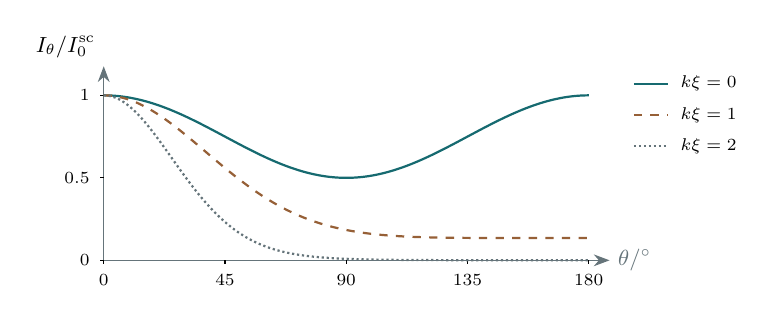
\begin{tikzpicture}[scale=.88,transform shape]
\draw[axis] (0,0.0)--(7.3,0.0) node[right] {$\theta/{}^\circ$};
\draw[axis] (0,0)--(0,2.8);
\node[above left] at (0,2.8) {$I_\theta/I_0^{\rm sc}$};
\draw[thin] (0.000000,0.0)--(0.000000,-0.06);\node[below,font=\scriptsize] at (0.000000,-0.08) {$ 0 $};
\draw[thin] (1.750000,0.0)--(1.750000,-0.06);\node[below,font=\scriptsize] at (1.750000,-0.08) {$ 45 $};
\draw[thin] (3.500000,0.0)--(3.500000,-0.06);\node[below,font=\scriptsize] at (3.500000,-0.08) {$ 90 $};
\draw[thin] (5.250000,0.0)--(5.250000,-0.06);\node[below,font=\scriptsize] at (5.250000,-0.08) {$ 135 $};
\draw[thin] (7.000000,0.0)--(7.000000,-0.06);\node[below,font=\scriptsize] at (7.000000,-0.08) {$ 180 $};
\draw[thin] (0,0.000000)--(-.06,0.000000);\node[left,font=\scriptsize] at (-.08,0.000000) {$ 0 $};
\draw[thin] (0,1.190476)--(-.06,1.190476);\node[left,font=\scriptsize] at (-.08,1.190476) {$ 0.5 $};
\draw[thin] (0,2.380952)--(-.06,2.380952);\node[left,font=\scriptsize] at (-.08,2.380952) {$ 1 $};
\draw[thick,color=accent] plot coordinates {(0.0000000,2.3809524) (0.0291667,2.3807484) (0.0583333,2.3801366) (0.0875000,2.3791175) (0.1166667,2.3776916) (0.1458333,2.3758600) (0.1750000,2.3736240) (0.2041667,2.3709851) (0.2333333,2.3679450) (0.2625000,2.3645059) (0.2916667,2.3606701) (0.3208333,2.3564403) (0.3500000,2.3518194) (0.3791667,2.3468104) (0.4083333,2.3414169) (0.4375000,2.3356426) (0.4666667,2.3294913) (0.4958333,2.3229674) (0.5250000,2.3160753) (0.5541667,2.3088197) (0.5833333,2.3012056) (0.6125000,2.2932382) (0.6416667,2.2849230) (0.6708333,2.2762656) (0.7000000,2.2672720) (0.7291667,2.2579484) (0.7583333,2.2483012) (0.7875000,2.2383369) (0.8166667,2.2280624) (0.8458333,2.2174847) (0.8750000,2.2066112) (0.9041667,2.1954492) (0.9333333,2.1840063) (0.9625000,2.1722905) (0.9916667,2.1603098) (1.0208333,2.1480723) (1.0500000,2.1355865) (1.0791667,2.1228609) (1.1083333,2.1099042) (1.1375000,2.0967253) (1.1666667,2.0833333) (1.1958333,2.0697374) (1.2250000,2.0559467) (1.2541667,2.0419709) (1.2833333,2.0278194) (1.3125000,2.0135020) (1.3416667,1.9990285) (1.3708333,1.9844088) (1.4000000,1.9696530) (1.4291667,1.9547710) (1.4583333,1.9397732) (1.4875000,1.9246699) (1.5166667,1.9094712) (1.5458333,1.8941878) (1.5750000,1.8788300) (1.6041667,1.8634084) (1.6333333,1.8479336) (1.6625000,1.8324161) (1.6916667,1.8168666) (1.7208333,1.8012958) (1.7500000,1.7857143) (1.7791667,1.7701328) (1.8083333,1.7545619) (1.8375000,1.7390124) (1.8666667,1.7234950) (1.8958333,1.7080201) (1.9250000,1.6925985) (1.9541667,1.6772408) (1.9833333,1.6619573) (2.0125000,1.6467587) (2.0416667,1.6316553) (2.0708333,1.6166575) (2.1000000,1.6017756) (2.1291667,1.5870197) (2.1583333,1.5724000) (2.1875000,1.5579265) (2.2166667,1.5436091) (2.2458333,1.5294577) (2.2750000,1.5154818) (2.3041667,1.5016912) (2.3333333,1.4880952) (2.3625000,1.4747032) (2.3916667,1.4615244) (2.4208333,1.4485677) (2.4500000,1.4358421) (2.4791667,1.4233563) (2.5083333,1.4111188) (2.5375000,1.3991381) (2.5666667,1.3874223) (2.5958333,1.3759794) (2.6250000,1.3648174) (2.6541667,1.3539438) (2.6833333,1.3433662) (2.7125000,1.3330917) (2.7416667,1.3231274) (2.7708333,1.3134802) (2.8000000,1.3041566) (2.8291667,1.2951630) (2.8583333,1.2865056) (2.8875000,1.2781904) (2.9166667,1.2702230) (2.9458333,1.2626089) (2.9750000,1.2553533) (3.0041667,1.2484611) (3.0333333,1.2419372) (3.0625000,1.2357860) (3.0916667,1.2300117) (3.1208333,1.2246182) (3.1500000,1.2196092) (3.1791667,1.2149883) (3.2083333,1.2107584) (3.2375000,1.2069227) (3.2666667,1.2034836) (3.2958333,1.2004435) (3.3250000,1.1978046) (3.3541667,1.1955685) (3.3833333,1.1937370) (3.4125000,1.1923111) (3.4416667,1.1912919) (3.4708333,1.1906802) (3.5000000,1.1904762) (3.5291667,1.1906802) (3.5583333,1.1912919) (3.5875000,1.1923111) (3.6166667,1.1937370) (3.6458333,1.1955685) (3.6750000,1.1978046) (3.7041667,1.2004435) (3.7333333,1.2034836) (3.7625000,1.2069227) (3.7916667,1.2107584) (3.8208333,1.2149883) (3.8500000,1.2196092) (3.8791667,1.2246182) (3.9083333,1.2300117) (3.9375000,1.2357860) (3.9666667,1.2419372) (3.9958333,1.2484611) (4.0250000,1.2553533) (4.0541667,1.2626089) (4.0833333,1.2702230) (4.1125000,1.2781904) (4.1416667,1.2865056) (4.1708333,1.2951630) (4.2000000,1.3041566) (4.2291667,1.3134802) (4.2583333,1.3231274) (4.2875000,1.3330917) (4.3166667,1.3433662) (4.3458333,1.3539438) (4.3750000,1.3648174) (4.4041667,1.3759794) (4.4333333,1.3874223) (4.4625000,1.3991381) (4.4916667,1.4111188) (4.5208333,1.4233563) (4.5500000,1.4358421) (4.5791667,1.4485677) (4.6083333,1.4615244) (4.6375000,1.4747032) (4.6666667,1.4880952) (4.6958333,1.5016912) (4.7250000,1.5154818) (4.7541667,1.5294577) (4.7833333,1.5436091) (4.8125000,1.5579265) (4.8416667,1.5724000) (4.8708333,1.5870197) (4.9000000,1.6017756) (4.9291667,1.6166575) (4.9583333,1.6316553) (4.9875000,1.6467587) (5.0166667,1.6619573) (5.0458333,1.6772408) (5.0750000,1.6925985) (5.1041667,1.7080201) (5.1333333,1.7234950) (5.1625000,1.7390124) (5.1916667,1.7545619) (5.2208333,1.7701328) (5.2500000,1.7857143) (5.2791667,1.8012958) (5.3083333,1.8168666) (5.3375000,1.8324161) (5.3666667,1.8479336) (5.3958333,1.8634084) (5.4250000,1.8788300) (5.4541667,1.8941878) (5.4833333,1.9094712) (5.5125000,1.9246699) (5.5416667,1.9397732) (5.5708333,1.9547710) (5.6000000,1.9696530) (5.6291667,1.9844088) (5.6583333,1.9990285) (5.6875000,2.0135020) (5.7166667,2.0278194) (5.7458333,2.0419709) (5.7750000,2.0559467) (5.8041667,2.0697374) (5.8333333,2.0833333) (5.8625000,2.0967253) (5.8916667,2.1099042) (5.9208333,2.1228609) (5.9500000,2.1355865) (5.9791667,2.1480723) (6.0083333,2.1603098) (6.0375000,2.1722905) (6.0666667,2.1840063) (6.0958333,2.1954492) (6.1250000,2.2066112) (6.1541667,2.2174847) (6.1833333,2.2280624) (6.2125000,2.2383369) (6.2416667,2.2483012) (6.2708333,2.2579484) (6.3000000,2.2672720) (6.3291667,2.2762656) (6.3583333,2.2849230) (6.3875000,2.2932382) (6.4166667,2.3012056) (6.4458333,2.3088197) (6.4750000,2.3160753) (6.5041667,2.3229674) (6.5333333,2.3294913) (6.5625000,2.3356426) (6.5916667,2.3414169) (6.6208333,2.3468104) (6.6500000,2.3518194) (6.6791667,2.3564403) (6.7083333,2.3606701) (6.7375000,2.3645059) (6.7666667,2.3679450) (6.7958333,2.3709851) (6.8250000,2.3736240) (6.8541667,2.3758600) (6.8833333,2.3776916) (6.9125000,2.3791175) (6.9416667,2.3801366) (6.9708333,2.3807484) (7.0000000,2.3809524)};
\draw[thick,color=accent] (7.65,2.55)--(8.15,2.55);\node[right,font=\scriptsize] at (8.2,2.55) {$k\xi=0$};
\draw[thick,dashed,color=warm] plot coordinates {(0.0000000,2.3809524) (0.0291667,2.3805445) (0.0583333,2.3793212) (0.0875000,2.3772840) (0.1166667,2.3744353) (0.1458333,2.3707786) (0.1750000,2.3663182) (0.2041667,2.3610594) (0.2333333,2.3550086) (0.2625000,2.3481729) (0.2916667,2.3405604) (0.3208333,2.3321802) (0.3500000,2.3230421) (0.3791667,2.3131569) (0.4083333,2.3025361) (0.4375000,2.2911923) (0.4666667,2.2791385) (0.4958333,2.2663889) (0.5250000,2.2529580) (0.5541667,2.2388612) (0.5833333,2.2241148) (0.6125000,2.2087354) (0.6416667,2.1927403) (0.6708333,2.1761476) (0.7000000,2.1589756) (0.7291667,2.1412435) (0.7583333,2.1229707) (0.7875000,2.1041771) (0.8166667,2.0848830) (0.8458333,2.0651092) (0.8750000,2.0448766) (0.9041667,2.0242067) (0.9333333,2.0031209) (0.9625000,1.9816411) (0.9916667,1.9597892) (1.0208333,1.9375874) (1.0500000,1.9150578) (1.0791667,1.8922229) (1.1083333,1.8691049) (1.1375000,1.8457261) (1.1666667,1.8221089) (1.1958333,1.7982755) (1.2250000,1.7742479) (1.2541667,1.7500481) (1.2833333,1.7256980) (1.3125000,1.7012191) (1.3416667,1.6766328) (1.3708333,1.6519603) (1.4000000,1.6272222) (1.4291667,1.6024391) (1.4583333,1.5776311) (1.4875000,1.5528181) (1.5166667,1.5280193) (1.5458333,1.5032538) (1.5750000,1.4785402) (1.6041667,1.4538964) (1.6333333,1.4293401) (1.6625000,1.4048884) (1.6916667,1.3805580) (1.7208333,1.3563649) (1.7500000,1.3323247) (1.7791667,1.3084523) (1.8083333,1.2847624) (1.8375000,1.2612687) (1.8666667,1.2379847) (1.8958333,1.2149230) (1.9250000,1.1920959) (1.9541667,1.1695149) (1.9833333,1.1471911) (2.0125000,1.1251348) (2.0416667,1.1033560) (2.0708333,1.0818639) (2.1000000,1.0606671) (2.1291667,1.0397737) (2.1583333,1.0191912) (2.1875000,0.9989266) (2.2166667,0.9789862) (2.2458333,0.9593759) (2.2750000,0.9401010) (2.3041667,0.9211661) (2.3333333,0.9025754) (2.3625000,0.8843327) (2.3916667,0.8664410) (2.4208333,0.8489031) (2.4500000,0.8317212) (2.4791667,0.8148969) (2.5083333,0.7984316) (2.5375000,0.7823259) (2.5666667,0.7665803) (2.5958333,0.7511947) (2.6250000,0.7361687) (2.6541667,0.7215015) (2.6833333,0.7071917) (2.7125000,0.6932378) (2.7416667,0.6796380) (2.7708333,0.6663899) (2.8000000,0.6534910) (2.8291667,0.6409384) (2.8583333,0.6287290) (2.8875000,0.6168593) (2.9166667,0.6053258) (2.9458333,0.5941244) (2.9750000,0.5832510) (3.0041667,0.5727014) (3.0333333,0.5624709) (3.0625000,0.5525549) (3.0916667,0.5429485) (3.1208333,0.5336466) (3.1500000,0.5246442) (3.1791667,0.5159358) (3.2083333,0.5075161) (3.2375000,0.4993796) (3.2666667,0.4915207) (3.2958333,0.4839337) (3.3250000,0.4766129) (3.3541667,0.4695526) (3.3833333,0.4627468) (3.4125000,0.4561897) (3.4416667,0.4498754) (3.4708333,0.4437980) (3.5000000,0.4379517) (3.5291667,0.4323305) (3.5583333,0.4269286) (3.5875000,0.4217400) (3.6166667,0.4167590) (3.6458333,0.4119797) (3.6750000,0.4073963) (3.7041667,0.4030033) (3.7333333,0.3987949) (3.7625000,0.3947654) (3.7916667,0.3909095) (3.8208333,0.3872216) (3.8500000,0.3836963) (3.8791667,0.3803283) (3.9083333,0.3771124) (3.9375000,0.3740435) (3.9666667,0.3711165) (3.9958333,0.3683264) (4.0250000,0.3656684) (4.0541667,0.3631377) (4.0833333,0.3607296) (4.1125000,0.3584396) (4.1416667,0.3562632) (4.1708333,0.3541959) (4.2000000,0.3522337) (4.2291667,0.3503722) (4.2583333,0.3486075) (4.2875000,0.3469356) (4.3166667,0.3453526) (4.3458333,0.3438548) (4.3750000,0.3424386) (4.4041667,0.3411005) (4.4333333,0.3398370) (4.4625000,0.3386449) (4.4916667,0.3375208) (4.5208333,0.3364617) (4.5500000,0.3354646) (4.5791667,0.3345265) (4.6083333,0.3336447) (4.6375000,0.3328163) (4.6666667,0.3320389) (4.6958333,0.3313099) (4.7250000,0.3306268) (4.7541667,0.3299872) (4.7833333,0.3293890) (4.8125000,0.3288300) (4.8416667,0.3283080) (4.8708333,0.3278211) (4.9000000,0.3273673) (4.9291667,0.3269448) (4.9583333,0.3265519) (4.9875000,0.3261868) (5.0166667,0.3258480) (5.0458333,0.3255338) (5.0750000,0.3252429) (5.1041667,0.3249737) (5.1333333,0.3247251) (5.1625000,0.3244956) (5.1916667,0.3242841) (5.2208333,0.3240894) (5.2500000,0.3239104) (5.2791667,0.3237461) (5.3083333,0.3235955) (5.3375000,0.3234576) (5.3666667,0.3233316) (5.3958333,0.3232166) (5.4250000,0.3231119) (5.4541667,0.3230166) (5.4833333,0.3229300) (5.5125000,0.3228516) (5.5416667,0.3227807) (5.5708333,0.3227166) (5.6000000,0.3226589) (5.6291667,0.3226070) (5.6583333,0.3225604) (5.6875000,0.3225187) (5.7166667,0.3224815) (5.7458333,0.3224483) (5.7750000,0.3224189) (5.8041667,0.3223928) (5.8333333,0.3223697) (5.8625000,0.3223494) (5.8916667,0.3223316) (5.9208333,0.3223160) (5.9500000,0.3223023) (5.9791667,0.3222905) (6.0083333,0.3222803) (6.0375000,0.3222715) (6.0666667,0.3222639) (6.0958333,0.3222574) (6.1250000,0.3222519) (6.1541667,0.3222473) (6.1833333,0.3222434) (6.2125000,0.3222401) (6.2416667,0.3222374) (6.2708333,0.3222352) (6.3000000,0.3222334) (6.3291667,0.3222319) (6.3583333,0.3222307) (6.3875000,0.3222298) (6.4166667,0.3222290) (6.4458333,0.3222285) (6.4750000,0.3222280) (6.5041667,0.3222277) (6.5333333,0.3222274) (6.5625000,0.3222273) (6.5916667,0.3222271) (6.6208333,0.3222270) (6.6500000,0.3222270) (6.6791667,0.3222269) (6.7083333,0.3222269) (6.7375000,0.3222269) (6.7666667,0.3222269) (6.7958333,0.3222269) (6.8250000,0.3222269) (6.8541667,0.3222269) (6.8833333,0.3222269) (6.9125000,0.3222269) (6.9416667,0.3222269) (6.9708333,0.3222269) (7.0000000,0.3222269)};
\draw[thick,dashed,color=warm] (7.65,2.0999999999999996)--(8.15,2.0999999999999996);\node[right,font=\scriptsize] at (8.2,2.0999999999999996) {$k\xi=1$};
\draw[densely dotted,thick,color=muted] plot coordinates {(0.0000000,2.3809524) (0.0291667,2.3799327) (0.0583333,2.3768764) (0.0875000,2.3717919) (0.1166667,2.3646931) (0.1458333,2.3555993) (0.1750000,2.3445354) (0.2041667,2.3315312) (0.2333333,2.3166220) (0.2625000,2.2998477) (0.2916667,2.2812533) (0.3208333,2.2608881) (0.3500000,2.2388058) (0.3791667,2.2150642) (0.4083333,2.1897249) (0.4375000,2.1628530) (0.4666667,2.1345169) (0.4958333,2.1047879) (0.5250000,2.0737400) (0.5541667,2.0414495) (0.5833333,2.0079945) (0.6125000,1.9734550) (0.6416667,1.9379123) (0.6708333,1.9014485) (0.7000000,1.8641467) (0.7291667,1.8260901) (0.7583333,1.7873621) (0.7875000,1.7480458) (0.8166667,1.7082237) (0.8458333,1.6679774) (0.8750000,1.6273877) (0.9041667,1.5865336) (0.9333333,1.5454927) (0.9625000,1.5043409) (0.9916667,1.4631516) (1.0208333,1.4219964) (1.0500000,1.3809441) (1.0791667,1.3400611) (1.1083333,1.2994109) (1.1375000,1.2590542) (1.1666667,1.2190487) (1.1958333,1.1794490) (1.2250000,1.1403065) (1.2541667,1.1016695) (1.2833333,1.0635829) (1.3125000,1.0260885) (1.3416667,0.9892246) (1.3708333,0.9530264) (1.4000000,0.9175257) (1.4291667,0.8827514) (1.4583333,0.8487288) (1.4875000,0.8154805) (1.5166667,0.7830257) (1.5458333,0.7513809) (1.5750000,0.7205598) (1.6041667,0.6905731) (1.6333333,0.6614290) (1.6625000,0.6331331) (1.6916667,0.6056887) (1.7208333,0.5790966) (1.7500000,0.5533556) (1.7791667,0.5284624) (1.8083333,0.5044117) (1.8375000,0.4811965) (1.8666667,0.4588080) (1.8958333,0.4372361) (1.9250000,0.4164692) (1.9541667,0.3964942) (1.9833333,0.3772971) (2.0125000,0.3588628) (2.0416667,0.3411752) (2.0708333,0.3242175) (2.1000000,0.3079721) (2.1291667,0.2924208) (2.1583333,0.2775451) (2.1875000,0.2633258) (2.2166667,0.2497436) (2.2458333,0.2367788) (2.2750000,0.2244118) (2.3041667,0.2126228) (2.3333333,0.2013918) (2.3625000,0.1906991) (2.3916667,0.1805252) (2.4208333,0.1708505) (2.4500000,0.1616557) (2.4791667,0.1529220) (2.5083333,0.1446305) (2.5375000,0.1367632) (2.5666667,0.1293018) (2.5958333,0.1222290) (2.6250000,0.1155276) (2.6541667,0.1091810) (2.6833333,0.1031728) (2.7125000,0.0974875) (2.7416667,0.0921098) (2.7708333,0.0870248) (2.8000000,0.0822185) (2.8291667,0.0776769) (2.8583333,0.0733870) (2.8875000,0.0693359) (2.9166667,0.0655114) (2.9458333,0.0619018) (2.9750000,0.0584957) (3.0041667,0.0552825) (3.0333333,0.0522518) (3.0625000,0.0493937) (3.0916667,0.0466989) (3.1208333,0.0441584) (3.1500000,0.0417635) (3.1791667,0.0395063) (3.2083333,0.0373789) (3.2375000,0.0353741) (3.2666667,0.0334847) (3.2958333,0.0317043) (3.3250000,0.0300266) (3.3541667,0.0284455) (3.3833333,0.0269555) (3.4125000,0.0255513) (3.4416667,0.0242278) (3.4708333,0.0229803) (3.5000000,0.0218043) (3.5291667,0.0206956) (3.5583333,0.0196502) (3.5875000,0.0186642) (3.6166667,0.0177343) (3.6458333,0.0168570) (3.6750000,0.0160292) (3.7041667,0.0152479) (3.7333333,0.0145103) (3.7625000,0.0138140) (3.7916667,0.0131563) (3.8208333,0.0125349) (3.8500000,0.0119478) (3.8791667,0.0113929) (3.9083333,0.0108682) (3.9375000,0.0103719) (3.9666667,0.0099024) (3.9958333,0.0094582) (4.0250000,0.0090376) (4.0541667,0.0086393) (4.0833333,0.0082620) (4.1125000,0.0079046) (4.1416667,0.0075657) (4.1708333,0.0072444) (4.2000000,0.0069396) (4.2291667,0.0066504) (4.2583333,0.0063759) (4.2875000,0.0061153) (4.3166667,0.0058677) (4.3458333,0.0056325) (4.3750000,0.0054089) (4.4041667,0.0051963) (4.4333333,0.0049941) (4.4625000,0.0048017) (4.4916667,0.0046186) (4.5208333,0.0044443) (4.5500000,0.0042783) (4.5791667,0.0041201) (4.6083333,0.0039693) (4.6375000,0.0038256) (4.6666667,0.0036886) (4.6958333,0.0035579) (4.7250000,0.0034332) (4.7541667,0.0033142) (4.7833333,0.0032005) (4.8125000,0.0030920) (4.8416667,0.0029884) (4.8708333,0.0028894) (4.9000000,0.0027947) (4.9291667,0.0027042) (4.9583333,0.0026177) (4.9875000,0.0025350) (5.0166667,0.0024558) (5.0458333,0.0023801) (5.0750000,0.0023076) (5.1041667,0.0022383) (5.1333333,0.0021719) (5.1625000,0.0021083) (5.1916667,0.0020474) (5.2208333,0.0019890) (5.2500000,0.0019331) (5.2791667,0.0018796) (5.3083333,0.0018283) (5.3375000,0.0017791) (5.3666667,0.0017319) (5.3958333,0.0016867) (5.4250000,0.0016434) (5.4541667,0.0016019) (5.4833333,0.0015620) (5.5125000,0.0015239) (5.5416667,0.0014872) (5.5708333,0.0014521) (5.6000000,0.0014184) (5.6291667,0.0013861) (5.6583333,0.0013551) (5.6875000,0.0013255) (5.7166667,0.0012970) (5.7458333,0.0012697) (5.7750000,0.0012435) (5.8041667,0.0012184) (5.8333333,0.0011944) (5.8625000,0.0011713) (5.8916667,0.0011493) (5.9208333,0.0011281) (5.9500000,0.0011079) (5.9791667,0.0010885) (6.0083333,0.0010700) (6.0375000,0.0010523) (6.0666667,0.0010353) (6.0958333,0.0010192) (6.1250000,0.0010037) (6.1541667,0.0009890) (6.1833333,0.0009749) (6.2125000,0.0009615) (6.2416667,0.0009487) (6.2708333,0.0009366) (6.3000000,0.0009251) (6.3291667,0.0009141) (6.3583333,0.0009038) (6.3875000,0.0008940) (6.4166667,0.0008847) (6.4458333,0.0008760) (6.4750000,0.0008678) (6.5041667,0.0008600) (6.5333333,0.0008528) (6.5625000,0.0008461) (6.5916667,0.0008399) (6.6208333,0.0008341) (6.6500000,0.0008288) (6.6791667,0.0008239) (6.7083333,0.0008195) (6.7375000,0.0008155) (6.7666667,0.0008120) (6.7958333,0.0008088) (6.8250000,0.0008061) (6.8541667,0.0008039) (6.8833333,0.0008020) (6.9125000,0.0008006) (6.9416667,0.0007995) (6.9708333,0.0007989) (7.0000000,0.0007987)};
\draw[densely dotted,thick,color=muted] (7.65,1.65)--(8.15,1.65);\node[right,font=\scriptsize] at (8.2,1.65) {$k\xi=2$};
\end{tikzpicture}
\figcaption{解图光5.9D\quad 高斯相关谱对较大角散射产生额外抑制，前向归一为1}
\end{minipage}\end{center}
在当前瑞利近似下，前向和后向的角因子均为2，$90^\circ$处为1。该处散射光完全沿垂直散射面的方向偏振；一般角度的两份输出强度分别按1与$\cos^2\theta$变化，线偏振度因而为$P=(I_\perp-I_\parallel)/(I_\perp+I_\parallel)=\sin^2\theta/(1+\cos^2\theta)$。$F_\rho$保留微元之间的位置相关，横向投影决定每一份输入的辐射方向性，两项共同给观察方向的强度。


\Needspace{13\baselineskip}

\pdfbookmark[2]{第 10 题 射电脉冲啁啾与电子密度}{q10}

\section*{第 10 题\quad 射电脉冲啁啾与电子密度}\label{q:10}

距离地球$L$的空间射电源，在同一时刻发出宽频带短脉冲。假设传播路径是均匀、无磁场、无碰撞的完全电离冷等离子体，传播频率高于等离子体截止频率。到达信号的角频率随接收时刻变化，局部斜率$\dd\omega/\dd t$已测得。由$L$、该时刻角频率$\omega$和斜率，导出电子平均数密度$N$的确定式；同时给出高频近似，并说明反演需要的发射条件。

\begin{center}\begin{minipage}{.98\linewidth}\centering
\begin{tikzpicture}[scale=.9,transform shape]
\fill (0.00000,0.00000) circle(.035);\node[left] at (0.00000,0.00000) {射电源};\draw[object] (7.00000,-1.50000)--(7.00000,1.80000);\node[above] at (7.00000,1.80000) {地球};\draw[motion] (0.00000,0.00000)--(2.00000,1.00000);
\draw[motion] (2.00000,1.00000)--(6.50000,1.00000);\node[above] at (3.80000,1.12000) {高频先到};\draw[motion] (0.00000,0.00000)--(2.00000,0.00000);
\draw[motion] (2.00000,0.00000)--(6.50000,0.00000);\node[above] at (3.80000,0.12000) {中心频率};\draw[motion] (0.00000,0.00000)--(2.00000,-1.00000);
\draw[motion] (2.00000,-1.00000)--(6.50000,-1.00000);\node[above] at (3.80000,-0.88000) {低频后到};\draw[<->,thin,color=muted] (0.00000,-2.00000)--(7.00000,-2.00000);\node[below] at (3.50000,-2.00000) {传播长度 $L$};\node[above] at (1.00000,2.00000) {共同发射时刻 $t_e$};
\end{tikzpicture}
\figcaption{图光5.10\quad 频率分量同时发射，群延迟使接收时间分开。}
\end{minipage}\end{center}

\Needspace{6\baselineskip}\subsection*{解答}


图光5.10把同一射电脉冲分成若干窄频段。采用均匀、无碰撞、无磁的冷等离子体模型，各频段在共同的发射时刻$t_e$出发。对每一窄频段，群速决定包络到达时间，整个宽带脉冲则随色散展开。电子数密度$N$先通过等离子体频率进入介电响应，传播支取$\omega>\omega_p$。

令$n=\sqrt{1-\omega_p^2/\omega^2}$，$k=\omega n/c$。材料参数$\omega_p$固定时，
\[
 \frac{\dd n}{\dd\omega}=\frac{\omega_p^2}{n\omega^3},\qquad
 \frac{\dd k}{\dd\omega}=\frac1c\left(n+\frac{\omega_p^2}{n\omega^2}\right)
 =\frac1{cn}.
\]
这里使用$n^2+\omega_p^2/\omega^2=1$，故
\[
\omega_p^2=\frac{Ne^2}{\varepsilon_0m_e},\quad
k=\frac1c\sqrt{\omega^2-\omega_p^2},\quad
v_g=\left(\frac{\dd k}{\dd\omega}\right)^{-1}
=c\sqrt{1-\frac{\omega_p^2}{\omega^2}}.
\]
若波包的传播相位写成$k(\omega)L-\omega(t-t_e)$，驻相条件为$L\,\dd k/\dd\omega=t-t_e$，于是到达时间为
\[
t(\omega)=t_e+\frac Lc
\left(1-\frac{\omega_p^2}{\omega^2}\right)^{-1/2}.
\]
解图光5.10B画出传播时间随频率的下降曲线。频率越高，群速越接近$c$，越早到达；低频端靠近传播下限，所需时间增大。相速度$c/n$用于等相位面，包络时间由上面的导数给出。
\begin{center}\begin{minipage}{.98\linewidth}\centering
\begin{tikzpicture}[scale=.88,transform shape]
\draw[axis] (0,0.0)--(7.3,0.0) node[right] {$\omega/\omega_p$};
\draw[axis] (0,0)--(0,2.8);
\node[above left] at (0,2.8) {$c(t-t_e)/L$};
\draw[thin] (0.000000,0.0)--(0.000000,-0.06);\node[below,font=\scriptsize] at (0.000000,-0.08) {$ 1.02 $};
\draw[thin] (1.723618,0.0)--(1.723618,-0.06);\node[below,font=\scriptsize] at (1.723618,-0.08) {$ 2 $};
\draw[thin] (3.482412,0.0)--(3.482412,-0.06);\node[below,font=\scriptsize] at (3.482412,-0.08) {$ 3 $};
\draw[thin] (5.241206,0.0)--(5.241206,-0.06);\node[below,font=\scriptsize] at (5.241206,-0.08) {$ 4 $};
\draw[thin] (7.000000,0.0)--(7.000000,-0.06);\node[below,font=\scriptsize] at (7.000000,-0.08) {$ 5 $};
\draw[thin] (0,0.000000)--(-.06,0.000000);\node[left,font=\scriptsize] at (-.08,0.000000) {$ 0 $};
\draw[thin] (0,0.454545)--(-.06,0.454545);\node[left,font=\scriptsize] at (-.08,0.454545) {$ 1 $};
\draw[thin] (0,1.363636)--(-.06,1.363636);\node[left,font=\scriptsize] at (-.08,1.363636) {$ 3 $};
\draw[thin] (0,2.272727)--(-.06,2.272727);\node[left,font=\scriptsize] at (-.08,2.272727) {$ 5 $};
\draw[thick,color=accent] plot coordinates {(0.0000000,2.3066771) (0.0291667,1.7261909) (0.0583333,1.4489140) (0.0875000,1.2797601) (0.1166667,1.1634811) (0.1458333,1.0776212) (0.1750000,1.0111155) (0.2041667,0.9578024) (0.2333333,0.9139460) (0.2625000,0.8771332) (0.2916667,0.8457279) (0.3208333,0.8185768) (0.3500000,0.7948411) (0.3791667,0.7738943) (0.4083333,0.7552580) (0.4375000,0.7385601) (0.4666667,0.7235059) (0.4958333,0.7098591) (0.5250000,0.6974277) (0.5541667,0.6860537) (0.5833333,0.6756059) (0.6125000,0.6659745) (0.6416667,0.6570667) (0.6708333,0.6488034) (0.7000000,0.6411170) (0.7291667,0.6339489) (0.7583333,0.6272486) (0.7875000,0.6209719) (0.8166667,0.6150801) (0.8458333,0.6095391) (0.8750000,0.6043188) (0.9041667,0.5993925) (0.9333333,0.5947364) (0.9625000,0.5903292) (0.9916667,0.5861518) (1.0208333,0.5821871) (1.0500000,0.5784195) (1.0791667,0.5748350) (1.1083333,0.5714210) (1.1375000,0.5681658) (1.1666667,0.5650590) (1.1958333,0.5620910) (1.2250000,0.5592528) (1.2541667,0.5565365) (1.2833333,0.5539346) (1.3125000,0.5514403) (1.3416667,0.5490474) (1.3708333,0.5467499) (1.4000000,0.5445425) (1.4291667,0.5424202) (1.4583333,0.5403784) (1.4875000,0.5384128) (1.5166667,0.5365194) (1.5458333,0.5346944) (1.5750000,0.5329344) (1.6041667,0.5312362) (1.6333333,0.5295966) (1.6625000,0.5280129) (1.6916667,0.5264824) (1.7208333,0.5250026) (1.7500000,0.5235711) (1.7791667,0.5221858) (1.8083333,0.5208445) (1.8375000,0.5195453) (1.8666667,0.5182864) (1.8958333,0.5170660) (1.9250000,0.5158825) (1.9541667,0.5147343) (1.9833333,0.5136200) (2.0125000,0.5125382) (2.0416667,0.5114875) (2.0708333,0.5104668) (2.1000000,0.5094747) (2.1291667,0.5085103) (2.1583333,0.5075725) (2.1875000,0.5066602) (2.2166667,0.5057724) (2.2458333,0.5049083) (2.2750000,0.5040670) (2.3041667,0.5032477) (2.3333333,0.5024495) (2.3625000,0.5016718) (2.3916667,0.5009137) (2.4208333,0.5001746) (2.4500000,0.4994539) (2.4791667,0.4987509) (2.5083333,0.4980650) (2.5375000,0.4973957) (2.5666667,0.4967424) (2.5958333,0.4961045) (2.6250000,0.4954816) (2.6541667,0.4948732) (2.6833333,0.4942788) (2.7125000,0.4936980) (2.7416667,0.4931303) (2.7708333,0.4925754) (2.8000000,0.4920329) (2.8291667,0.4915023) (2.8583333,0.4909833) (2.8875000,0.4904756) (2.9166667,0.4899788) (2.9458333,0.4894926) (2.9750000,0.4890168) (3.0041667,0.4885509) (3.0333333,0.4880947) (3.0625000,0.4876480) (3.0916667,0.4872104) (3.1208333,0.4867818) (3.1500000,0.4863618) (3.1791667,0.4859503) (3.2083333,0.4855469) (3.2375000,0.4851515) (3.2666667,0.4847639) (3.2958333,0.4843838) (3.3250000,0.4840110) (3.3541667,0.4836454) (3.3833333,0.4832868) (3.4125000,0.4829350) (3.4416667,0.4825898) (3.4708333,0.4822510) (3.5000000,0.4819185) (3.5291667,0.4815921) (3.5583333,0.4812717) (3.5875000,0.4809571) (3.6166667,0.4806482) (3.6458333,0.4803448) (3.6750000,0.4800468) (3.7041667,0.4797541) (3.7333333,0.4794666) (3.7625000,0.4791840) (3.7916667,0.4789064) (3.8208333,0.4786335) (3.8500000,0.4783654) (3.8791667,0.4781017) (3.9083333,0.4778426) (3.9375000,0.4775878) (3.9666667,0.4773372) (3.9958333,0.4770909) (4.0250000,0.4768486) (4.0541667,0.4766102) (4.0833333,0.4763758) (4.1125000,0.4761451) (4.1416667,0.4759182) (4.1708333,0.4756949) (4.2000000,0.4754752) (4.2291667,0.4752590) (4.2583333,0.4750461) (4.2875000,0.4748366) (4.3166667,0.4746304) (4.3458333,0.4744273) (4.3750000,0.4742274) (4.4041667,0.4740306) (4.4333333,0.4738367) (4.4625000,0.4736458) (4.4916667,0.4734578) (4.5208333,0.4732725) (4.5500000,0.4730901) (4.5791667,0.4729103) (4.6083333,0.4727332) (4.6375000,0.4725587) (4.6666667,0.4723868) (4.6958333,0.4722173) (4.7250000,0.4720503) (4.7541667,0.4718857) (4.7833333,0.4717234) (4.8125000,0.4715635) (4.8416667,0.4714058) (4.8708333,0.4712503) (4.9000000,0.4710971) (4.9291667,0.4709459) (4.9583333,0.4707969) (4.9875000,0.4706499) (5.0166667,0.4705049) (5.0458333,0.4703619) (5.0750000,0.4702208) (5.1041667,0.4700817) (5.1333333,0.4699445) (5.1625000,0.4698090) (5.1916667,0.4696754) (5.2208333,0.4695436) (5.2500000,0.4694135) (5.2791667,0.4692851) (5.3083333,0.4691584) (5.3375000,0.4690334) (5.3666667,0.4689099) (5.3958333,0.4687881) (5.4250000,0.4686678) (5.4541667,0.4685491) (5.4833333,0.4684319) (5.5125000,0.4683162) (5.5416667,0.4682019) (5.5708333,0.4680891) (5.6000000,0.4679777) (5.6291667,0.4678676) (5.6583333,0.4677590) (5.6875000,0.4676517) (5.7166667,0.4675457) (5.7458333,0.4674410) (5.7750000,0.4673376) (5.8041667,0.4672354) (5.8333333,0.4671345) (5.8625000,0.4670348) (5.8916667,0.4669362) (5.9208333,0.4668389) (5.9500000,0.4667427) (5.9791667,0.4666477) (6.0083333,0.4665537) (6.0375000,0.4664609) (6.0666667,0.4663692) (6.0958333,0.4662785) (6.1250000,0.4661889) (6.1541667,0.4661003) (6.1833333,0.4660128) (6.2125000,0.4659262) (6.2416667,0.4658407) (6.2708333,0.4657561) (6.3000000,0.4656724) (6.3291667,0.4655897) (6.3583333,0.4655080) (6.3875000,0.4654271) (6.4166667,0.4653472) (6.4458333,0.4652681) (6.4750000,0.4651899) (6.5041667,0.4651126) (6.5333333,0.4650362) (6.5625000,0.4649605) (6.5916667,0.4648857) (6.6208333,0.4648117) (6.6500000,0.4647385) (6.6791667,0.4646661) (6.7083333,0.4645945) (6.7375000,0.4645236) (6.7666667,0.4644535) (6.7958333,0.4643841) (6.8250000,0.4643155) (6.8541667,0.4642476) (6.8833333,0.4641804) (6.9125000,0.4641139) (6.9416667,0.4640481) (6.9708333,0.4639830) (7.0000000,0.4639185)};
\end{tikzpicture}
\figcaption{解图光5.10B\quad 低频群速较小，传播所需时间较长}
\end{minipage}\end{center}
求导时先写$y=\omega_p^2/\omega^2$，其导数为$\dd y/\dd\omega=-2\omega_p^2/\omega^3$，而$\dd(1-y)^{-1/2}/\dd y=\tfrac12(1-y)^{-3/2}$。两项相乘得到
\[
\frac{\dd t}{\dd\omega}
=-\frac Lc\,\frac{\omega_p^2}{\omega^3}
\left(1-\frac{\omega_p^2}{\omega^2}\right)^{-3/2}<0.
\]
接收记录通常给频率随到达时间的变化率，定义正量$s=-\dd\omega/\dd t$。对这条单调到达曲线取导数的倒数，再保留负号，得
\[
s=\frac{c\omega^3}{L\omega_p^2}
\left(1-\frac{\omega_p^2}{\omega^2}\right)^{3/2}.
\]
解图光5.10A改以接收时间为横轴画频率轨迹，显示测得的负斜率。反演使用轨迹上该点的频率$\omega$、斜率$s$与传播距离$L$。
\begin{center}\begin{minipage}{.98\linewidth}\centering
\begin{tikzpicture}[scale=.88,transform shape]
\draw[axis] (0,0.0)--(7.3,0.0) node[right] {$c(t-t_e)/L$};
\draw[axis] (0,0)--(0,2.8);
\node[above left] at (0,2.8) {$\omega/\omega_p$};
\draw[thin] (0.000000,0.0)--(0.000000,-0.06);\node[below,font=\scriptsize] at (0.000000,-0.08) {$ 1.02 $};
\draw[thin] (1.696970,0.0)--(1.696970,-0.06);\node[below,font=\scriptsize] at (1.696970,-0.08) {$ 1.5 $};
\draw[thin] (3.464646,0.0)--(3.464646,-0.06);\node[below,font=\scriptsize] at (3.464646,-0.08) {$ 2 $};
\draw[thin] (7.000000,0.0)--(7.000000,-0.06);\node[below,font=\scriptsize] at (7.000000,-0.08) {$ 3 $};
\draw[thin] (0,0.000000)--(-.06,0.000000);\node[left,font=\scriptsize] at (-.08,0.000000) {$ 0 $};
\draw[thin] (0,0.454545)--(-.06,0.454545);\node[left,font=\scriptsize] at (-.08,0.454545) {$ 1 $};
\draw[thin] (0,1.363636)--(-.06,1.363636);\node[left,font=\scriptsize] at (-.08,1.363636) {$ 3 $};
\draw[thin] (0,2.272727)--(-.06,2.272727);\node[left,font=\scriptsize] at (-.08,2.272727) {$ 5 $};
\draw[thick,color=accent] plot coordinates {(0.0000000,2.3066771) (0.0291667,1.9525676) (0.0583333,1.7280567) (0.0875000,1.5699039) (0.1166667,1.4510196) (0.1458333,1.3576150) (0.1750000,1.2818376) (0.2041667,1.2188451) (0.2333333,1.1654691) (0.2625000,1.1195382) (0.2916667,1.0795083) (0.3208333,1.0442473) (0.3500000,1.0129044) (0.3791667,0.9848258) (0.4083333,0.9595001) (0.4375000,0.9365208) (0.4666667,0.9155601) (0.4958333,0.8963505) (0.5250000,0.8786712) (0.5541667,0.8623380) (0.5833333,0.8471964) (0.6125000,0.8331150) (0.6416667,0.8199818) (0.6708333,0.8077006) (0.7000000,0.7961879) (0.7291667,0.7853714) (0.7583333,0.7751876) (0.7875000,0.7655808) (0.8166667,0.7565019) (0.8458333,0.7479073) (0.8750000,0.7397581) (0.9041667,0.7320199) (0.9333333,0.7246614) (0.9625000,0.7176548) (0.9916667,0.7109750) (1.0208333,0.7045991) (1.0500000,0.6985065) (1.0791667,0.6926784) (1.1083333,0.6870977) (1.1375000,0.6817488) (1.1666667,0.6766174) (1.1958333,0.6716902) (1.2250000,0.6669553) (1.2541667,0.6624015) (1.2833333,0.6580185) (1.3125000,0.6537969) (1.3416667,0.6497278) (1.3708333,0.6458032) (1.4000000,0.6420154) (1.4291667,0.6383574) (1.4583333,0.6348227) (1.4875000,0.6314052) (1.5166667,0.6280991) (1.5458333,0.6248990) (1.5750000,0.6218001) (1.6041667,0.6187976) (1.6333333,0.6158871) (1.6625000,0.6130645) (1.6916667,0.6103259) (1.7208333,0.6076677) (1.7500000,0.6050863) (1.7791667,0.6025787) (1.8083333,0.6001416) (1.8375000,0.5977722) (1.8666667,0.5954678) (1.8958333,0.5932258) (1.9250000,0.5910437) (1.9541667,0.5889191) (1.9833333,0.5868500) (2.0125000,0.5848342) (2.0416667,0.5828697) (2.0708333,0.5809546) (2.1000000,0.5790871) (2.1291667,0.5772655) (2.1583333,0.5754882) (2.1875000,0.5737536) (2.2166667,0.5720603) (2.2458333,0.5704068) (2.2750000,0.5687918) (2.3041667,0.5672140) (2.3333333,0.5656721) (2.3625000,0.5641650) (2.3916667,0.5626916) (2.4208333,0.5612507) (2.4500000,0.5598414) (2.4791667,0.5584627) (2.5083333,0.5571135) (2.5375000,0.5557931) (2.5666667,0.5545004) (2.5958333,0.5532348) (2.6250000,0.5519953) (2.6541667,0.5507812) (2.6833333,0.5495918) (2.7125000,0.5484264) (2.7416667,0.5472842) (2.7708333,0.5461646) (2.8000000,0.5450669) (2.8291667,0.5439907) (2.8583333,0.5429351) (2.8875000,0.5418998) (2.9166667,0.5408841) (2.9458333,0.5398875) (2.9750000,0.5389095) (3.0041667,0.5379496) (3.0333333,0.5370074) (3.0625000,0.5360823) (3.0916667,0.5351740) (3.1208333,0.5342819) (3.1500000,0.5334058) (3.1791667,0.5325451) (3.2083333,0.5316996) (3.2375000,0.5308687) (3.2666667,0.5300522) (3.2958333,0.5292498) (3.3250000,0.5284610) (3.3541667,0.5276856) (3.3833333,0.5269232) (3.4125000,0.5261735) (3.4416667,0.5254362) (3.4708333,0.5247111) (3.5000000,0.5239978) (3.5291667,0.5232961) (3.5583333,0.5226057) (3.5875000,0.5219263) (3.6166667,0.5212578) (3.6458333,0.5205998) (3.6750000,0.5199522) (3.7041667,0.5193147) (3.7333333,0.5186870) (3.7625000,0.5180690) (3.7916667,0.5174605) (3.8208333,0.5168612) (3.8500000,0.5162710) (3.8791667,0.5156897) (3.9083333,0.5151171) (3.9375000,0.5145529) (3.9666667,0.5139971) (3.9958333,0.5134494) (4.0250000,0.5129097) (4.0541667,0.5123778) (4.0833333,0.5118536) (4.1125000,0.5113369) (4.1416667,0.5108276) (4.1708333,0.5103255) (4.2000000,0.5098304) (4.2291667,0.5093423) (4.2583333,0.5088610) (4.2875000,0.5083863) (4.3166667,0.5079182) (4.3458333,0.5074565) (4.3750000,0.5070011) (4.4041667,0.5065518) (4.4333333,0.5061086) (4.4625000,0.5056714) (4.4916667,0.5052399) (4.5208333,0.5048142) (4.5500000,0.5043941) (4.5791667,0.5039796) (4.6083333,0.5035704) (4.6375000,0.5031665) (4.6666667,0.5027679) (4.6958333,0.5023744) (4.7250000,0.5019859) (4.7541667,0.5016024) (4.7833333,0.5012237) (4.8125000,0.5008498) (4.8416667,0.5004806) (4.8708333,0.5001160) (4.9000000,0.4997559) (4.9291667,0.4994003) (4.9583333,0.4990491) (4.9875000,0.4987021) (5.0166667,0.4983594) (5.0458333,0.4980208) (5.0750000,0.4976863) (5.1041667,0.4973559) (5.1333333,0.4970293) (5.1625000,0.4967067) (5.1916667,0.4963879) (5.2208333,0.4960728) (5.2500000,0.4957615) (5.2791667,0.4954538) (5.3083333,0.4951496) (5.3375000,0.4948490) (5.3666667,0.4945519) (5.3958333,0.4942581) (5.4250000,0.4939678) (5.4541667,0.4936807) (5.4833333,0.4933969) (5.5125000,0.4931162) (5.5416667,0.4928388) (5.5708333,0.4925644) (5.6000000,0.4922931) (5.6291667,0.4920248) (5.6583333,0.4917594) (5.6875000,0.4914970) (5.7166667,0.4912374) (5.7458333,0.4909807) (5.7750000,0.4907268) (5.8041667,0.4904756) (5.8333333,0.4902271) (5.8625000,0.4899813) (5.8916667,0.4897381) (5.9208333,0.4894975) (5.9500000,0.4892594) (5.9791667,0.4890239) (6.0083333,0.4887908) (6.0375000,0.4885602) (6.0666667,0.4883319) (6.0958333,0.4881061) (6.1250000,0.4878825) (6.1541667,0.4876613) (6.1833333,0.4874424) (6.2125000,0.4872257) (6.2416667,0.4870112) (6.2708333,0.4867989) (6.3000000,0.4865887) (6.3291667,0.4863806) (6.3583333,0.4861746) (6.3875000,0.4859707) (6.4166667,0.4857689) (6.4458333,0.4855690) (6.4750000,0.4853711) (6.5041667,0.4851751) (6.5333333,0.4849811) (6.5625000,0.4847889) (6.5916667,0.4845987) (6.6208333,0.4844103) (6.6500000,0.4842237) (6.6791667,0.4840389) (6.7083333,0.4838558) (6.7375000,0.4836746) (6.7666667,0.4834950) (6.7958333,0.4833172) (6.8250000,0.4831410) (6.8541667,0.4829665) (6.8833333,0.4827937) (6.9125000,0.4826225) (6.9416667,0.4824528) (6.9708333,0.4822848) (7.0000000,0.4821183)};
\end{tikzpicture}
\figcaption{解图光5.10A\quad 按接收时间读取频率的下降轨迹}
\end{minipage}\end{center}
引入无量纲$y=\omega_p^2/\omega^2$和$\eta=sL/(c\omega)$，则密度由
\[
\boxed{\eta=\frac{(1-y)^{3/2}}y,\quad 0<y<1},
\qquad
\boxed{N=\frac{\varepsilon_0m_e}{e^2}\omega^2y}.
\]
确定。函数$f(y)=(1-y)^{3/2}/y$的导数为
\[
\frac{\dd}{\dd y}\frac{(1-y)^{3/2}}y
=-\frac{\sqrt{1-y}(1+y/2)}{y^2}<0.
\]
它在$0<y<1$连续递减，$y\to0$时趋于无穷，$y\to1$时趋于零，所以任意$\eta>0$恰给一个传播支的密度。解图光5.10C画$f(y)$及一个测量水平值，可在此区间用二分求根。等价的立方方程为$\eta^2y^2=(1-y)^3$，它的物理解仍在同一区间选取。
\begin{center}\begin{minipage}{.98\linewidth}\centering
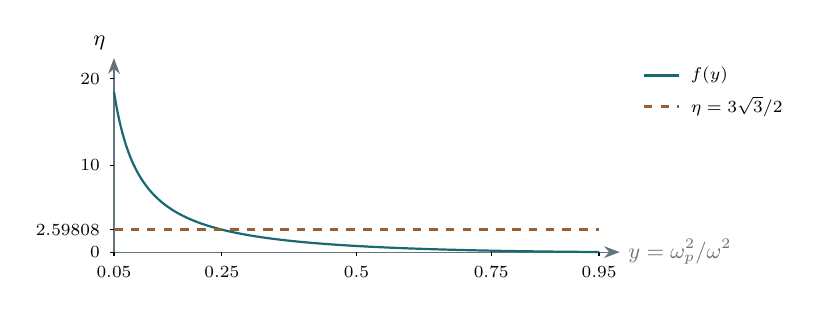
\begin{tikzpicture}[scale=.88,transform shape]
\draw[axis] (0,0.0)--(7.3,0.0) node[right] {$y=\omega_p^2/\omega^2$};
\draw[axis] (0,0)--(0,2.8);
\node[above left] at (0,2.8) {$\eta$};
\draw[thin] (0.000000,0.0)--(0.000000,-0.06);\node[below,font=\scriptsize] at (0.000000,-0.08) {$ 0.05 $};
\draw[thin] (1.555556,0.0)--(1.555556,-0.06);\node[below,font=\scriptsize] at (1.555556,-0.08) {$ 0.25 $};
\draw[thin] (3.500000,0.0)--(3.500000,-0.06);\node[below,font=\scriptsize] at (3.500000,-0.08) {$ 0.5 $};
\draw[thin] (5.444444,0.0)--(5.444444,-0.06);\node[below,font=\scriptsize] at (5.444444,-0.08) {$ 0.75 $};
\draw[thin] (7.000000,0.0)--(7.000000,-0.06);\node[below,font=\scriptsize] at (7.000000,-0.08) {$ 0.95 $};
\draw[thin] (0,0.000000)--(-.06,0.000000);\node[left,font=\scriptsize] at (-.08,0.000000) {$ 0 $};
\draw[thin] (0,0.324760)--(-.06,0.324760);\node[left,font=\scriptsize] at (-.08,0.324760) {$ 2.59808 $};
\draw[thin] (0,1.250000)--(-.06,1.250000);\node[left,font=\scriptsize] at (-.08,1.250000) {$ 10 $};
\draw[thin] (0,2.500000)--(-.06,2.500000);\node[left,font=\scriptsize] at (-.08,2.500000) {$ 20 $};
\draw[thick,color=accent] plot coordinates {(0.0000000,2.3148637) (0.0291667,2.1406240) (0.0583333,1.9891348) (0.0875000,1.8562174) (0.1166667,1.7386576) (0.1458333,1.6339424) (0.1750000,1.5400786) (0.2041667,1.4554653) (0.2333333,1.3788016) (0.2625000,1.3090197) (0.2916667,1.2452349) (0.3208333,1.1867077) (0.3500000,1.1328157) (0.3791667,1.0830308) (0.4083333,1.0369023) (0.4375000,0.9940430) (0.4666667,0.9541185) (0.4958333,0.9168388) (0.5250000,0.8819505) (0.5541667,0.8492318) (0.5833333,0.8184876) (0.6125000,0.7895451) (0.6416667,0.7622516) (0.6708333,0.7364709) (0.7000000,0.7120814) (0.7291667,0.6889743) (0.7583333,0.6670518) (0.7875000,0.6462258) (0.8166667,0.6264168) (0.8458333,0.6075526) (0.8750000,0.5895680) (0.9041667,0.5724033) (0.9333333,0.5560044) (0.9625000,0.5403217) (0.9916667,0.5253098) (1.0208333,0.5109271) (1.0500000,0.4971354) (1.0791667,0.4838994) (1.1083333,0.4711868) (1.1375000,0.4589674) (1.1666667,0.4472136) (1.1958333,0.4358997) (1.2250000,0.4250018) (1.2541667,0.4144979) (1.2833333,0.4043673) (1.3125000,0.3945908) (1.3416667,0.3851506) (1.3708333,0.3760299) (1.4000000,0.3672132) (1.4291667,0.3586858) (1.4583333,0.3504339) (1.4875000,0.3424449) (1.5166667,0.3347067) (1.5458333,0.3272078) (1.5750000,0.3199377) (1.6041667,0.3128863) (1.6333333,0.3060443) (1.6625000,0.2994026) (1.6916667,0.2929528) (1.7208333,0.2866871) (1.7500000,0.2805978) (1.7791667,0.2746780) (1.8083333,0.2689208) (1.8375000,0.2633199) (1.8666667,0.2578692) (1.8958333,0.2525631) (1.9250000,0.2473959) (1.9541667,0.2423626) (1.9833333,0.2374583) (2.0125000,0.2326782) (2.0416667,0.2280180) (2.0708333,0.2234732) (2.1000000,0.2190400) (2.1291667,0.2147144) (2.1583333,0.2104927) (2.1875000,0.2063715) (2.2166667,0.2023474) (2.2458333,0.1984172) (2.2750000,0.1945777) (2.3041667,0.1908261) (2.3333333,0.1871596) (2.3625000,0.1835754) (2.3916667,0.1800710) (2.4208333,0.1766439) (2.4500000,0.1732917) (2.4791667,0.1700122) (2.5083333,0.1668032) (2.5375000,0.1636626) (2.5666667,0.1605883) (2.5958333,0.1575785) (2.6250000,0.1546313) (2.6541667,0.1517449) (2.6833333,0.1489176) (2.7125000,0.1461477) (2.7416667,0.1434336) (2.7708333,0.1407739) (2.8000000,0.1381670) (2.8291667,0.1356114) (2.8583333,0.1331059) (2.8875000,0.1306492) (2.9166667,0.1282398) (2.9458333,0.1258767) (2.9750000,0.1235585) (3.0041667,0.1212842) (3.0333333,0.1190527) (3.0625000,0.1168629) (3.0916667,0.1147137) (3.1208333,0.1126042) (3.1500000,0.1105334) (3.1791667,0.1085003) (3.2083333,0.1065040) (3.2375000,0.1045437) (3.2666667,0.1026186) (3.2958333,0.1007277) (3.3250000,0.0988704) (3.3541667,0.0970457) (3.3833333,0.0952531) (3.4125000,0.0934917) (3.4416667,0.0917609) (3.4708333,0.0900600) (3.5000000,0.0883883) (3.5291667,0.0867453) (3.5583333,0.0851301) (3.5875000,0.0835424) (3.6166667,0.0819814) (3.6458333,0.0804467) (3.6750000,0.0789376) (3.7041667,0.0774536) (3.7333333,0.0759943) (3.7625000,0.0745591) (3.7916667,0.0731474) (3.8208333,0.0717590) (3.8500000,0.0703932) (3.8791667,0.0690496) (3.9083333,0.0677279) (3.9375000,0.0664274) (3.9666667,0.0651480) (3.9958333,0.0638891) (4.0250000,0.0626503) (4.0541667,0.0614313) (4.0833333,0.0602318) (4.1125000,0.0590512) (4.1416667,0.0578894) (4.1708333,0.0567459) (4.2000000,0.0556204) (4.2291667,0.0545125) (4.2583333,0.0534221) (4.2875000,0.0523487) (4.3166667,0.0512921) (4.3458333,0.0502519) (4.3750000,0.0492279) (4.4041667,0.0482198) (4.4333333,0.0472274) (4.4625000,0.0462503) (4.4916667,0.0452883) (4.5208333,0.0443411) (4.5500000,0.0434086) (4.5791667,0.0424904) (4.6083333,0.0415864) (4.6375000,0.0406962) (4.6666667,0.0398198) (4.6958333,0.0389568) (4.7250000,0.0381070) (4.7541667,0.0372703) (4.7833333,0.0364465) (4.8125000,0.0356353) (4.8416667,0.0348365) (4.8708333,0.0340500) (4.9000000,0.0332756) (4.9291667,0.0325131) (4.9583333,0.0317623) (4.9875000,0.0310231) (5.0166667,0.0302953) (5.0458333,0.0295787) (5.0750000,0.0288731) (5.1041667,0.0281785) (5.1333333,0.0274947) (5.1625000,0.0268214) (5.1916667,0.0261587) (5.2208333,0.0255062) (5.2500000,0.0248640) (5.2791667,0.0242318) (5.3083333,0.0236096) (5.3375000,0.0229971) (5.3666667,0.0223943) (5.3958333,0.0218011) (5.4250000,0.0212173) (5.4541667,0.0206429) (5.4833333,0.0200776) (5.5125000,0.0195215) (5.5416667,0.0189743) (5.5708333,0.0184360) (5.6000000,0.0179065) (5.6291667,0.0173857) (5.6583333,0.0168735) (5.6875000,0.0163698) (5.7166667,0.0158744) (5.7458333,0.0153874) (5.7750000,0.0149086) (5.8041667,0.0144380) (5.8333333,0.0139754) (5.8625000,0.0135208) (5.8916667,0.0130742) (5.9208333,0.0126353) (5.9500000,0.0122042) (5.9791667,0.0117808) (6.0083333,0.0113651) (6.0375000,0.0109569) (6.0666667,0.0105561) (6.0958333,0.0101629) (6.1250000,0.0097770) (6.1541667,0.0093984) (6.1833333,0.0090272) (6.2125000,0.0086631) (6.2416667,0.0083062) (6.2708333,0.0079565) (6.3000000,0.0076138) (6.3291667,0.0072782) (6.3583333,0.0069497) (6.3875000,0.0066281) (6.4166667,0.0063135) (6.4458333,0.0060058) (6.4750000,0.0057050) (6.5041667,0.0054110) (6.5333333,0.0051240) (6.5625000,0.0048438) (6.5916667,0.0045705) (6.6208333,0.0043040) (6.6500000,0.0040443) (6.6791667,0.0037915) (6.7083333,0.0035456) (6.7375000,0.0033065) (6.7666667,0.0030744) (6.7958333,0.0028492) (6.8250000,0.0026309) (6.8541667,0.0024197) (6.8833333,0.0022155) (6.9125000,0.0020185) (6.9416667,0.0018286) (6.9708333,0.0016462) (7.0000000,0.0014711)};
\draw[thick,color=accent] (7.65,2.55)--(8.15,2.55);\node[right,font=\scriptsize] at (8.2,2.55) {$f(y)$};
\draw[thick,dashed,color=warm] plot coordinates {(0.0000000,0.3247595) (0.0291667,0.3247595) (0.0583333,0.3247595) (0.0875000,0.3247595) (0.1166667,0.3247595) (0.1458333,0.3247595) (0.1750000,0.3247595) (0.2041667,0.3247595) (0.2333333,0.3247595) (0.2625000,0.3247595) (0.2916667,0.3247595) (0.3208333,0.3247595) (0.3500000,0.3247595) (0.3791667,0.3247595) (0.4083333,0.3247595) (0.4375000,0.3247595) (0.4666667,0.3247595) (0.4958333,0.3247595) (0.5250000,0.3247595) (0.5541667,0.3247595) (0.5833333,0.3247595) (0.6125000,0.3247595) (0.6416667,0.3247595) (0.6708333,0.3247595) (0.7000000,0.3247595) (0.7291667,0.3247595) (0.7583333,0.3247595) (0.7875000,0.3247595) (0.8166667,0.3247595) (0.8458333,0.3247595) (0.8750000,0.3247595) (0.9041667,0.3247595) (0.9333333,0.3247595) (0.9625000,0.3247595) (0.9916667,0.3247595) (1.0208333,0.3247595) (1.0500000,0.3247595) (1.0791667,0.3247595) (1.1083333,0.3247595) (1.1375000,0.3247595) (1.1666667,0.3247595) (1.1958333,0.3247595) (1.2250000,0.3247595) (1.2541667,0.3247595) (1.2833333,0.3247595) (1.3125000,0.3247595) (1.3416667,0.3247595) (1.3708333,0.3247595) (1.4000000,0.3247595) (1.4291667,0.3247595) (1.4583333,0.3247595) (1.4875000,0.3247595) (1.5166667,0.3247595) (1.5458333,0.3247595) (1.5750000,0.3247595) (1.6041667,0.3247595) (1.6333333,0.3247595) (1.6625000,0.3247595) (1.6916667,0.3247595) (1.7208333,0.3247595) (1.7500000,0.3247595) (1.7791667,0.3247595) (1.8083333,0.3247595) (1.8375000,0.3247595) (1.8666667,0.3247595) (1.8958333,0.3247595) (1.9250000,0.3247595) (1.9541667,0.3247595) (1.9833333,0.3247595) (2.0125000,0.3247595) (2.0416667,0.3247595) (2.0708333,0.3247595) (2.1000000,0.3247595) (2.1291667,0.3247595) (2.1583333,0.3247595) (2.1875000,0.3247595) (2.2166667,0.3247595) (2.2458333,0.3247595) (2.2750000,0.3247595) (2.3041667,0.3247595) (2.3333333,0.3247595) (2.3625000,0.3247595) (2.3916667,0.3247595) (2.4208333,0.3247595) (2.4500000,0.3247595) (2.4791667,0.3247595) (2.5083333,0.3247595) (2.5375000,0.3247595) (2.5666667,0.3247595) (2.5958333,0.3247595) (2.6250000,0.3247595) (2.6541667,0.3247595) (2.6833333,0.3247595) (2.7125000,0.3247595) (2.7416667,0.3247595) (2.7708333,0.3247595) (2.8000000,0.3247595) (2.8291667,0.3247595) (2.8583333,0.3247595) (2.8875000,0.3247595) (2.9166667,0.3247595) (2.9458333,0.3247595) (2.9750000,0.3247595) (3.0041667,0.3247595) (3.0333333,0.3247595) (3.0625000,0.3247595) (3.0916667,0.3247595) (3.1208333,0.3247595) (3.1500000,0.3247595) (3.1791667,0.3247595) (3.2083333,0.3247595) (3.2375000,0.3247595) (3.2666667,0.3247595) (3.2958333,0.3247595) (3.3250000,0.3247595) (3.3541667,0.3247595) (3.3833333,0.3247595) (3.4125000,0.3247595) (3.4416667,0.3247595) (3.4708333,0.3247595) (3.5000000,0.3247595) (3.5291667,0.3247595) (3.5583333,0.3247595) (3.5875000,0.3247595) (3.6166667,0.3247595) (3.6458333,0.3247595) (3.6750000,0.3247595) (3.7041667,0.3247595) (3.7333333,0.3247595) (3.7625000,0.3247595) (3.7916667,0.3247595) (3.8208333,0.3247595) (3.8500000,0.3247595) (3.8791667,0.3247595) (3.9083333,0.3247595) (3.9375000,0.3247595) (3.9666667,0.3247595) (3.9958333,0.3247595) (4.0250000,0.3247595) (4.0541667,0.3247595) (4.0833333,0.3247595) (4.1125000,0.3247595) (4.1416667,0.3247595) (4.1708333,0.3247595) (4.2000000,0.3247595) (4.2291667,0.3247595) (4.2583333,0.3247595) (4.2875000,0.3247595) (4.3166667,0.3247595) (4.3458333,0.3247595) (4.3750000,0.3247595) (4.4041667,0.3247595) (4.4333333,0.3247595) (4.4625000,0.3247595) (4.4916667,0.3247595) (4.5208333,0.3247595) (4.5500000,0.3247595) (4.5791667,0.3247595) (4.6083333,0.3247595) (4.6375000,0.3247595) (4.6666667,0.3247595) (4.6958333,0.3247595) (4.7250000,0.3247595) (4.7541667,0.3247595) (4.7833333,0.3247595) (4.8125000,0.3247595) (4.8416667,0.3247595) (4.8708333,0.3247595) (4.9000000,0.3247595) (4.9291667,0.3247595) (4.9583333,0.3247595) (4.9875000,0.3247595) (5.0166667,0.3247595) (5.0458333,0.3247595) (5.0750000,0.3247595) (5.1041667,0.3247595) (5.1333333,0.3247595) (5.1625000,0.3247595) (5.1916667,0.3247595) (5.2208333,0.3247595) (5.2500000,0.3247595) (5.2791667,0.3247595) (5.3083333,0.3247595) (5.3375000,0.3247595) (5.3666667,0.3247595) (5.3958333,0.3247595) (5.4250000,0.3247595) (5.4541667,0.3247595) (5.4833333,0.3247595) (5.5125000,0.3247595) (5.5416667,0.3247595) (5.5708333,0.3247595) (5.6000000,0.3247595) (5.6291667,0.3247595) (5.6583333,0.3247595) (5.6875000,0.3247595) (5.7166667,0.3247595) (5.7458333,0.3247595) (5.7750000,0.3247595) (5.8041667,0.3247595) (5.8333333,0.3247595) (5.8625000,0.3247595) (5.8916667,0.3247595) (5.9208333,0.3247595) (5.9500000,0.3247595) (5.9791667,0.3247595) (6.0083333,0.3247595) (6.0375000,0.3247595) (6.0666667,0.3247595) (6.0958333,0.3247595) (6.1250000,0.3247595) (6.1541667,0.3247595) (6.1833333,0.3247595) (6.2125000,0.3247595) (6.2416667,0.3247595) (6.2708333,0.3247595) (6.3000000,0.3247595) (6.3291667,0.3247595) (6.3583333,0.3247595) (6.3875000,0.3247595) (6.4166667,0.3247595) (6.4458333,0.3247595) (6.4750000,0.3247595) (6.5041667,0.3247595) (6.5333333,0.3247595) (6.5625000,0.3247595) (6.5916667,0.3247595) (6.6208333,0.3247595) (6.6500000,0.3247595) (6.6791667,0.3247595) (6.7083333,0.3247595) (6.7375000,0.3247595) (6.7666667,0.3247595) (6.7958333,0.3247595) (6.8250000,0.3247595) (6.8541667,0.3247595) (6.8833333,0.3247595) (6.9125000,0.3247595) (6.9416667,0.3247595) (6.9708333,0.3247595) (7.0000000,0.3247595)};
\draw[thick,dashed,color=warm] (7.65,2.0999999999999996)--(8.15,2.0999999999999996);\node[right,font=\scriptsize] at (8.2,2.0999999999999996) {$\eta=3\sqrt3/2$};
\end{tikzpicture}
\figcaption{解图光5.10C\quad 单调函数在传播区内给唯一密度}
\end{minipage}\end{center}
高频区$y\ll1$时，按$(1-y)^{-1/2}=1+\tfrac12y+\tfrac38y^2+\cdots$展开，保留首个色散项，
\[
t-t_e\simeq\frac Lc+\frac{L\omega_p^2}{2c\omega^2},\quad
s\simeq\frac{c\omega^3}{L\omega_p^2},
\]
代$\omega_p^2=Ne^2/(\varepsilon_0m_e)$，得到显式近似
\[
\boxed{N\simeq\frac{\varepsilon_0m_ec}{e^2L}
\frac{\omega^3}{s}
=-\frac{\varepsilon_0m_ec\omega^3}{e^2L(\dd\omega/\dd t)}}.
\]
用这项近似得到的密度计算$\omega_p/\omega$，便可估计后续修正。相同精确斜率若放入高频反演式，其结果满足$N_{\rm app}/N=(1-y)^{-3/2}$。解图光5.10D给这一比例；例如$y=0.01$时高估约1.52\%，靠近低频端时采用前面的精确反演。
\begin{center}\begin{minipage}{.98\linewidth}\centering
\begin{tikzpicture}[scale=.88,transform shape]
\draw[axis] (0,0)--(7.3,0) node[right] {$y$};
\draw[axis] (0,0)--(0,2.8);
\node[above left] at (0,2.8) {$N_{\rm app}/N$};
\draw[thin] (0.000000,0)--(0.000000,-0.06);\node[below,font=\scriptsize] at (0.000000,-0.08) {$ 0 $};
\draw[thin] (2.333333,0)--(2.333333,-0.06);\node[below,font=\scriptsize] at (2.333333,-0.08) {$ 0.2 $};
\draw[thin] (4.666667,0)--(4.666667,-0.06);\node[below,font=\scriptsize] at (4.666667,-0.08) {$ 0.4 $};
\draw[thin] (7.000000,0)--(7.000000,-0.06);\node[below,font=\scriptsize] at (7.000000,-0.08) {$ 0.6 $};
\draw[thin] (0,0.000000)--(-.06,0.000000);\node[left,font=\scriptsize] at (-.08,0.000000) {$ 1 $};
\draw[thin] (0,0.806452)--(-.06,0.806452);\node[left,font=\scriptsize] at (-.08,0.806452) {$ 2 $};
\draw[thin] (0,1.612903)--(-.06,1.612903);\node[left,font=\scriptsize] at (-.08,1.612903) {$ 3 $};
\draw[thin] (0,2.419355)--(-.06,2.419355);\node[left,font=\scriptsize] at (-.08,2.419355) {$ 4 $};
\draw[thick,color=accent] plot coordinates {(0.0000000,0.0000000) (0.0291667,0.0030337) (0.0583333,0.0060864) (0.0875000,0.0091584) (0.1166667,0.0122498) (0.1458333,0.0153607) (0.1750000,0.0184914) (0.2041667,0.0216421) (0.2333333,0.0248128) (0.2625000,0.0280039) (0.2916667,0.0312154) (0.3208333,0.0344475) (0.3500000,0.0377005) (0.3791667,0.0409745) (0.4083333,0.0442698) (0.4375000,0.0475864) (0.4666667,0.0509247) (0.4958333,0.0542847) (0.5250000,0.0576668) (0.5541667,0.0610711) (0.5833333,0.0644978) (0.6125000,0.0679471) (0.6416667,0.0714192) (0.6708333,0.0749144) (0.7000000,0.0784328) (0.7291667,0.0819747) (0.7583333,0.0855403) (0.7875000,0.0891298) (0.8166667,0.0927434) (0.8458333,0.0963814) (0.8750000,0.1000440) (0.9041667,0.1037315) (0.9333333,0.1074440) (0.9625000,0.1111818) (0.9916667,0.1149451) (1.0208333,0.1187343) (1.0500000,0.1225495) (1.0791667,0.1263910) (1.1083333,0.1302590) (1.1375000,0.1341539) (1.1666667,0.1380758) (1.1958333,0.1420250) (1.2250000,0.1460018) (1.2541667,0.1500065) (1.2833333,0.1540394) (1.3125000,0.1581007) (1.3416667,0.1621906) (1.3708333,0.1663096) (1.4000000,0.1704578) (1.4291667,0.1746356) (1.4583333,0.1788433) (1.4875000,0.1830811) (1.5166667,0.1873494) (1.5458333,0.1916485) (1.5750000,0.1959786) (1.6041667,0.2003402) (1.6333333,0.2047334) (1.6625000,0.2091587) (1.6916667,0.2136164) (1.7208333,0.2181068) (1.7500000,0.2226303) (1.7791667,0.2271871) (1.8083333,0.2317776) (1.8375000,0.2364022) (1.8666667,0.2410613) (1.8958333,0.2457552) (1.9250000,0.2504842) (1.9541667,0.2552487) (1.9833333,0.2600492) (2.0125000,0.2648859) (2.0416667,0.2697593) (2.0708333,0.2746698) (2.1000000,0.2796177) (2.1291667,0.2846035) (2.1583333,0.2896275) (2.1875000,0.2946902) (2.2166667,0.2997920) (2.2458333,0.3049334) (2.2750000,0.3101146) (2.3041667,0.3153363) (2.3333333,0.3205988) (2.3625000,0.3259025) (2.3916667,0.3312480) (2.4208333,0.3366357) (2.4500000,0.3420660) (2.4791667,0.3475395) (2.5083333,0.3530566) (2.5375000,0.3586178) (2.5666667,0.3642236) (2.5958333,0.3698744) (2.6250000,0.3755709) (2.6541667,0.3813135) (2.6833333,0.3871028) (2.7125000,0.3929393) (2.7416667,0.3988234) (2.7708333,0.4047559) (2.8000000,0.4107371) (2.8291667,0.4167678) (2.8583333,0.4228484) (2.8875000,0.4289796) (2.9166667,0.4351619) (2.9458333,0.4413959) (2.9750000,0.4476823) (3.0041667,0.4540216) (3.0333333,0.4604145) (3.0625000,0.4668617) (3.0916667,0.4733637) (3.1208333,0.4799213) (3.1500000,0.4865350) (3.1791667,0.4932056) (3.2083333,0.4999337) (3.2375000,0.5067202) (3.2666667,0.5135655) (3.2958333,0.5204706) (3.3250000,0.5274360) (3.3541667,0.5344627) (3.3833333,0.5415512) (3.4125000,0.5487024) (3.4416667,0.5559170) (3.4708333,0.5631959) (3.5000000,0.5705399) (3.5291667,0.5779497) (3.5583333,0.5854262) (3.5875000,0.5929702) (3.6166667,0.6005827) (3.6458333,0.6082644) (3.6750000,0.6160162) (3.7041667,0.6238391) (3.7333333,0.6317340) (3.7625000,0.6397018) (3.7916667,0.6477434) (3.8208333,0.6558598) (3.8500000,0.6640521) (3.8791667,0.6723210) (3.9083333,0.6806678) (3.9375000,0.6890934) (3.9666667,0.6975989) (3.9958333,0.7061852) (4.0250000,0.7148536) (4.0541667,0.7236051) (4.0833333,0.7324409) (4.1125000,0.7413620) (4.1416667,0.7503696) (4.1708333,0.7594649) (4.2000000,0.7686492) (4.2291667,0.7779236) (4.2583333,0.7872893) (4.2875000,0.7967477) (4.3166667,0.8063000) (4.3458333,0.8159476) (4.3750000,0.8256917) (4.4041667,0.8355337) (4.4333333,0.8454751) (4.4625000,0.8555172) (4.4916667,0.8656615) (4.5208333,0.8759093) (4.5500000,0.8862623) (4.5791667,0.8967219) (4.6083333,0.9072896) (4.6375000,0.9179671) (4.6666667,0.9287560) (4.6958333,0.9396578) (4.7250000,0.9506742) (4.7541667,0.9618070) (4.7833333,0.9730578) (4.8125000,0.9844285) (4.8416667,0.9959207) (4.8708333,1.0075364) (4.9000000,1.0192774) (4.9291667,1.0311456) (4.9583333,1.0431430) (4.9875000,1.0552714) (5.0166667,1.0675330) (5.0458333,1.0799298) (5.0750000,1.0924639) (5.1041667,1.1051374) (5.1333333,1.1179525) (5.1625000,1.1309114) (5.1916667,1.1440164) (5.2208333,1.1572699) (5.2500000,1.1706741) (5.2791667,1.1842315) (5.3083333,1.1979445) (5.3375000,1.2118158) (5.3666667,1.2258477) (5.3958333,1.2400430) (5.4250000,1.2544044) (5.4541667,1.2689345) (5.4833333,1.2836361) (5.5125000,1.2985121) (5.5416667,1.3135655) (5.5708333,1.3287991) (5.6000000,1.3442160) (5.6291667,1.3598194) (5.6583333,1.3756123) (5.6875000,1.3915981) (5.7166667,1.4077800) (5.7458333,1.4241615) (5.7750000,1.4407459) (5.8041667,1.4575369) (5.8333333,1.4745380) (5.8625000,1.4917530) (5.8916667,1.5091856) (5.9208333,1.5268397) (5.9500000,1.5447193) (5.9791667,1.5628284) (6.0083333,1.5811711) (6.0375000,1.5997518) (6.0666667,1.6185747) (6.0958333,1.6376443) (6.1250000,1.6569652) (6.1541667,1.6765420) (6.1833333,1.6963794) (6.2125000,1.7164824) (6.2416667,1.7368560) (6.2708333,1.7575052) (6.3000000,1.7784354) (6.3291667,1.7996519) (6.3583333,1.8211603) (6.3875000,1.8429661) (6.4166667,1.8650752) (6.4458333,1.8874936) (6.4750000,1.9102272) (6.5041667,1.9332824) (6.5333333,1.9566655) (6.5625000,1.9803832) (6.5916667,2.0044421) (6.6208333,2.0288492) (6.6500000,2.0536116) (6.6791667,2.0787365) (6.7083333,2.1042315) (6.7375000,2.1301041) (6.7666667,2.1563623) (6.7958333,2.1830142) (6.8250000,2.2100681) (6.8541667,2.2375325) (6.8833333,2.2654162) (6.9125000,2.2937283) (6.9416667,2.3224779) (6.9708333,2.3516746) (7.0000000,2.3813283)};
\end{tikzpicture}
\figcaption{解图光5.10D\quad 高频近似省去的因子使反演密度偏高，纵轴从1起}
\end{minipage}\end{center}
若发射时刻随频率变化，观测时间为$t_{\rm obs}=t_e(\omega)+L/v_g(\omega)$，其导数包含$t'_e(\omega)$，需把发射规律和传播延迟共同拟合。若路径密度随位置变化，在各处均满足高频近似、且射线路径固定时，把每一段的群延迟相加，得到相对真空的延迟
\[
\Delta t(\omega)\simeq\frac{e^2}{2\varepsilon_0m_ec\omega^2}
\int_0^L N(z)\dd z.
\]
因此首阶色散测量确定电子柱密度$\int N(z)\dd z$，以已知$L$相除得到路径平均密度。均匀模型的精确反演与变密度路径的高频平均各有对应条件；两段路径具有相同柱密度时，首阶延迟相同，更高阶项才包含密度平方等额外信息。


\Needspace{13\baselineskip}

\pdfbookmark[2]{第 11 题 吸收系数测量与表面反射}{q11}

\section*{第 11 题\quad 吸收系数测量与表面反射}\label{q:11}

强度$I_0$的单色光从空气垂直入射厚度$l$的有色玻璃，玻璃折射率$n=1.5$，强度吸收系数为$\alpha$。（1）忽略多重反射，求透射强度与入射强度之比。（2）忽略表面反射损失会产生多大的相对误差？明确误差以哪个量为分母，并给小反射率的一阶结果。（3）设计消除表面反射影响的吸收系数测量方法，说明需要保持哪些条件。

\begin{center}\begin{minipage}{.98\linewidth}\centering
\begin{tikzpicture}[scale=.9,transform shape]
\draw[object] (2.00000,-1.50000)--(2.00000,1.80000)--(5.00000,1.80000)--(5.00000,-1.50000)--(2.00000,-1.50000);\node[above] at (3.50000,1.80000) {$n=1.5,\alpha$};\draw[motion] (0.00000,0.00000)--(2.00000,0.00000);
\draw[motion] (2.00000,0.00000)--(5.00000,0.00000);
\draw[motion] (5.00000,0.00000)--(7.00000,0.00000);\node[below] at (0.50000,-0.35000) {$I_0$};\node[above] at (6.40000,0.10000) {$I_t$};\draw[force] (2.00000,0.35000)--(0.50000,0.35000);\draw[force] (5.00000,-0.40000)--(3.50000,-0.40000);\draw[<->,thin,color=muted] (2.00000,-2.00000)--(5.00000,-2.00000);\node[below] at (3.50000,-2.00000) {$l$};
\end{tikzpicture}
\figcaption{图光5.11\quad 光经历入口反射、体吸收与出口反射。}
\end{minipage}\end{center}

\Needspace{6\baselineskip}\subsection*{解答}


图光5.11按入口、体内传播、出口标出三段过程。题设$\alpha$定义为强度吸收系数，即材料内传播$l$后光强乘$e^{-\alpha l}$，相应场振幅乘$e^{-\alpha l/2}$。令 $k_0=2\pi/\lambda_0$，把强度吸收系数写成复折射率的虚部 $\kappa=\alpha/(2k_0)$。本题在界面处采用 $\kappa\ll n$ 的近似，用题给实折射率计算空气与玻璃两向的法向反射率。材料内即使 $\alpha l$ 不小，仍保留完整的指数衰减。这个近似下两向的反射率均为
\[
R=\left(\frac{n-1}{n+1}\right)^2
=\left(\frac{0.5}{2.5}\right)^2=0.04.
\]
把第一次穿出玻璃的光单独接收。入口反射$RI_0$后，进入材料的光强为$I_{\rm in}=(1-R)I_0$；传播到出口前为$I_l=(1-R)I_0e^{-\alpha l}$；出口又反射$RI_l$，所以空气中的透射光强为$I_t=(1-R)I_l$。由此
\[
\boxed{T\equiv\frac{I_t}{I_0}=(1-R)^2e^{-\alpha l}
=0.9216e^{-\alpha l}}.
\]
解图光5.11A把每一步对应的因子标在同一光路上。电场透射幅度的两个方向分别为$t_{01}=2/(1+n)=0.8$与$t_{10}=2n/(1+n)=1.2$，它们各自转成功率时还含介质波导纳。最终输入输出都在空气中，场乘积 $t_{01}t_{10}=0.96$ 取平方，与两个能量因子 $0.96^2$ 一致。若界面也需保留吸收，用 $\widetilde n=n+i\kappa$ 分别写出图A的两次场透射。首次透过率的界面常因子为
\[
K=\left|\frac{2}{1+\widetilde n}\frac{2\widetilde n}{1+\widetilde n}\right|^2
 =\left|\frac{4\widetilde n}{(1+\widetilde n)^2}\right|^2 .
\]
传播仍只乘 $e^{-\alpha l}$，因此只收集首次透射时，两厚度的 $T_j=K e^{-\alpha l_j}$ 相除仍能消去同一个 $K$。
\begin{center}\begin{minipage}{.98\linewidth}\centering
\begin{tikzpicture}[scale=.9,transform shape]
\fill[accent!8] (2,-1.2) rectangle (5,1.8);
\draw[object] (2,-1.2)--(2,1.8);\draw[object] (5,-1.2)--(5,1.8);
\draw[motion] (-.8,.4)--(1.8,.4) node[midway,above] {$I_0$};
\draw[motion] (2.2,.4)--(4.8,.4) node[midway,above] {$I_{\rm in}e^{-\alpha l}$};
\draw[motion] (5.2,.4)--(8,.4) node[midway,above] {$I_t$};
\draw[force,color=warm] (2,.4)--(.4,.4) node[pos=.65,below] {$RI_0$};
\draw[force,color=warm] (5,.4)--(3.4,.4) node[pos=.55,below] {$RI_l$};
\node[above] at (2,2) {$\times(1-R)$};\node[above] at (5,2) {$\times(1-R)$};
\draw[<->] (2,-1.5)--(5,-1.5) node[midway,below] {$l$};
\node[below] at (7,-.2) {$T=(1-R)^2e^{-\alpha l}$};
\end{tikzpicture}
\figcaption{解图光5.11A\quad 首次透射依次经过入口、体吸收和出口}
\end{minipage}\end{center}
记第二问省去反射的预测为$T_0=e^{-\alpha l}$，与实际透过率相减，得到
\[
T_0-T=[1-(1-R)^2]T_0=(2R-R^2)T_0.
\]
用$T_0$作分母，减少比例为$(T_0-T)/T_0=2R-R^2=7.84\%$；若以实际透过率$T$作分母，预测的相对高估为
\[
\frac{T_0-T}{T}=\frac1{(1-R)^2}-1=8.5069\%.
\]
两种精确分母约定在$R\ll1$时都给$2R\simeq8\%$。这是透过率的误差；若由透过率再反演吸收系数，对数还会引入厚度。将测量$T$放入$\alpha_{\rm app}=-(\ln T)/l$，得
\[
\boxed{\alpha_{\rm app}=\alpha-\frac{2\ln(1-R)}l
=\alpha+\frac{0.081644}{l}}.
\]
因此$\alpha$的相对高估为$[-2\ln(1-R)]/(\alpha l)$。解图光5.11C以$\alpha l$为横轴画这个比例；薄片或弱吸收材料中，同样的表面损失对吸收系数的相对影响较大。
\begin{center}\begin{minipage}{.98\linewidth}\centering
\begin{tikzpicture}[scale=.88,transform shape]
\draw[axis] (0,0.0)--(7.3,0.0) node[right] {$\alpha l$};
\draw[axis] (0,0)--(0,2.8);
\node[above left] at (0,2.8) {$(\alpha_{\rm app}-\alpha)/\alpha$};
\draw[thin] (0.000000,0.0)--(0.000000,-0.06);\node[below,font=\scriptsize] at (0.000000,-0.08) {$ 0.05 $};
\draw[thin] (1.105263,0.0)--(1.105263,-0.06);\node[below,font=\scriptsize] at (1.105263,-0.08) {$ 0.2 $};
\draw[thin] (3.315789,0.0)--(3.315789,-0.06);\node[below,font=\scriptsize] at (3.315789,-0.08) {$ 0.5 $};
\draw[thin] (7.000000,0.0)--(7.000000,-0.06);\node[below,font=\scriptsize] at (7.000000,-0.08) {$ 1 $};
\draw[thin] (0,0.000000)--(-.06,0.000000);\node[left,font=\scriptsize] at (-.08,0.000000) {$ 0 $};
\draw[thin] (0,0.735294)--(-.06,0.735294);\node[left,font=\scriptsize] at (-.08,0.735294) {$ 0.5 $};
\draw[thin] (0,1.470588)--(-.06,1.470588);\node[left,font=\scriptsize] at (-.08,1.470588) {$ 1 $};
\draw[thin] (0,2.205882)--(-.06,2.205882);\node[left,font=\scriptsize] at (-.08,2.205882) {$ 1.5 $};
\draw[thick,color=accent] plot coordinates {(0.0000000,2.4012938) (0.0291667,2.2251371) (0.0583333,2.0730594) (0.0875000,1.9404394) (0.1166667,1.8237674) (0.1458333,1.7203299) (0.1750000,1.6279958) (0.2041667,1.5450684) (0.2333333,1.4701799) (0.2625000,1.4022154) (0.2916667,1.3402570) (0.3208333,1.2835423) (0.3500000,1.2314327) (0.3791667,1.1833891) (0.4083333,1.1389536) (0.4375000,1.0977343) (0.4666667,1.0593943) (0.4958333,1.0236421) (0.5250000,0.9902242) (0.5541667,0.9589193) (0.5833333,0.9295331) (0.6125000,0.9018944) (0.6416667,0.8758518) (0.6708333,0.8512711) (0.7000000,0.8280323) (0.7291667,0.8060287) (0.7583333,0.7851642) (0.7875000,0.7653526) (0.8166667,0.7465162) (0.8458333,0.7285847) (0.8750000,0.7114945) (0.9041667,0.6951876) (0.9333333,0.6796115) (0.9625000,0.6647180) (0.9916667,0.6504633) (1.0208333,0.6368072) (1.0500000,0.6237127) (1.0791667,0.6111458) (1.1083333,0.5990754) (1.1375000,0.5874725) (1.1666667,0.5763105) (1.1958333,0.5655648) (1.2250000,0.5552124) (1.2541667,0.5452323) (1.2833333,0.5356046) (1.3125000,0.5263110) (1.3416667,0.5173344) (1.3708333,0.5086589) (1.4000000,0.5002695) (1.4291667,0.4921524) (1.4583333,0.4842945) (1.4875000,0.4766836) (1.5166667,0.4693082) (1.5458333,0.4621576) (1.5750000,0.4552216) (1.6041667,0.4484907) (1.6333333,0.4419559) (1.6625000,0.4356089) (1.6916667,0.4294415) (1.7208333,0.4234464) (1.7500000,0.4176163) (1.7791667,0.4119446) (1.8083333,0.4064249) (1.8375000,0.4010512) (1.8666667,0.3958177) (1.8958333,0.3907190) (1.9250000,0.3857500) (1.9541667,0.3809058) (1.9833333,0.3761818) (2.0125000,0.3715735) (2.0416667,0.3670768) (2.0708333,0.3626875) (2.1000000,0.3584021) (2.1291667,0.3542167) (2.1583333,0.3501279) (2.1875000,0.3461324) (2.2166667,0.3422271) (2.2458333,0.3384090) (2.2750000,0.3346751) (2.3041667,0.3310227) (2.3333333,0.3274492) (2.3625000,0.3239519) (2.3916667,0.3205286) (2.4208333,0.3171769) (2.4500000,0.3138946) (2.4791667,0.3106795) (2.5083333,0.3075296) (2.5375000,0.3044430) (2.5666667,0.3014176) (2.5958333,0.2984518) (2.6250000,0.2955439) (2.6541667,0.2926920) (2.6833333,0.2898946) (2.7125000,0.2871502) (2.7416667,0.2844573) (2.7708333,0.2818144) (2.8000000,0.2792202) (2.8291667,0.2766733) (2.8583333,0.2741725) (2.8875000,0.2717164) (2.9166667,0.2693040) (2.9458333,0.2669340) (2.9750000,0.2646054) (3.0041667,0.2623170) (3.0333333,0.2600679) (3.0625000,0.2578571) (3.0916667,0.2556835) (3.1208333,0.2535462) (3.1500000,0.2514444) (3.1791667,0.2493771) (3.2083333,0.2473436) (3.2375000,0.2453429) (3.2666667,0.2433744) (3.2958333,0.2414372) (3.3250000,0.2395306) (3.3541667,0.2376538) (3.3833333,0.2358063) (3.4125000,0.2339872) (3.4416667,0.2321960) (3.4708333,0.2304320) (3.5000000,0.2286946) (3.5291667,0.2269833) (3.5583333,0.2252973) (3.5875000,0.2236362) (3.6166667,0.2219994) (3.6458333,0.2203864) (3.6750000,0.2187967) (3.7041667,0.2172297) (3.7333333,0.2156851) (3.7625000,0.2141622) (3.7916667,0.2126607) (3.8208333,0.2111801) (3.8500000,0.2097200) (3.8791667,0.2082799) (3.9083333,0.2068595) (3.9375000,0.2054583) (3.9666667,0.2040760) (3.9958333,0.2027121) (4.0250000,0.2013664) (4.0541667,0.2000384) (4.0833333,0.1987278) (4.1125000,0.1974342) (4.1416667,0.1961574) (4.1708333,0.1948970) (4.2000000,0.1936527) (4.2291667,0.1924242) (4.2583333,0.1912112) (4.2875000,0.1900134) (4.3166667,0.1888304) (4.3458333,0.1876622) (4.3750000,0.1865083) (4.4041667,0.1853684) (4.4333333,0.1842425) (4.4625000,0.1831301) (4.4916667,0.1820311) (4.5208333,0.1809452) (4.5500000,0.1798722) (4.5791667,0.1788118) (4.6083333,0.1777639) (4.6375000,0.1767282) (4.6666667,0.1757044) (4.6958333,0.1746925) (4.7250000,0.1736921) (4.7541667,0.1727032) (4.7833333,0.1717254) (4.8125000,0.1707587) (4.8416667,0.1698027) (4.8708333,0.1688575) (4.9000000,0.1679226) (4.9291667,0.1669981) (4.9583333,0.1660837) (4.9875000,0.1651793) (5.0166667,0.1642846) (5.0458333,0.1633996) (5.0750000,0.1625241) (5.1041667,0.1616579) (5.1333333,0.1608009) (5.1625000,0.1599530) (5.1916667,0.1591139) (5.2208333,0.1582836) (5.2500000,0.1574619) (5.2791667,0.1566487) (5.3083333,0.1558438) (5.3375000,0.1550472) (5.3666667,0.1542587) (5.3958333,0.1534782) (5.4250000,0.1527055) (5.4541667,0.1519406) (5.4833333,0.1511832) (5.5125000,0.1504334) (5.5416667,0.1496910) (5.5708333,0.1489559) (5.6000000,0.1482280) (5.6291667,0.1475072) (5.6583333,0.1467933) (5.6875000,0.1460863) (5.7166667,0.1453861) (5.7458333,0.1446926) (5.7750000,0.1440056) (5.8041667,0.1433252) (5.8333333,0.1426511) (5.8625000,0.1419834) (5.8916667,0.1413219) (5.9208333,0.1406665) (5.9500000,0.1400171) (5.9791667,0.1393738) (6.0083333,0.1387363) (6.0375000,0.1381046) (6.0666667,0.1374787) (6.0958333,0.1368583) (6.1250000,0.1362436) (6.1541667,0.1356344) (6.1833333,0.1350306) (6.2125000,0.1344321) (6.2416667,0.1338389) (6.2708333,0.1332510) (6.3000000,0.1326682) (6.3291667,0.1320904) (6.3583333,0.1315177) (6.3875000,0.1309499) (6.4166667,0.1303870) (6.4458333,0.1298289) (6.4750000,0.1292756) (6.5041667,0.1287269) (6.5333333,0.1281829) (6.5625000,0.1276435) (6.5916667,0.1271086) (6.6208333,0.1265782) (6.6500000,0.1260522) (6.6791667,0.1255305) (6.7083333,0.1250131) (6.7375000,0.1245000) (6.7666667,0.1239911) (6.7958333,0.1234863) (6.8250000,0.1229856) (6.8541667,0.1224890) (6.8833333,0.1219963) (6.9125000,0.1215076) (6.9416667,0.1210228) (6.9708333,0.1205418) (7.0000000,0.1200647)};
\end{tikzpicture}
\figcaption{解图光5.11C\quad 同一表面损失对较弱体吸收产生更大的相对参数误差}
\end{minipage}\end{center}
第三问取同一材料、相同表面状态的两块玻璃，厚度$l_1<l_2$。在同一波长、入射方向及偏振下，分别用入射光归一化测得$T_1,T_2$，则
\[
T_1=(1-R)^2e^{-\alpha l_1},\qquad
T_2=(1-R)^2e^{-\alpha l_2}.
\]
两式相除给$T_1/T_2=e^{\alpha(l_2-l_1)}$，取对数得到
\[
\boxed{\alpha=\frac{\ln(T_1/T_2)}{l_2-l_1}}.
\]
解图光5.11B以无量纲厚度$u=\alpha l$画出$\ln T=2\ln(1-R)-u$，图中斜率为$-1$。实验把实测厚度$l$作横坐标时，斜率为$-\alpha$，共同表面因子仍进入截距。厚度差直接测量；若入射源随时间变化，用同步参考探测器分别归一化两次透射强度。抛光状态、镀层、温度和材料相同使两次测量具有同一个界面因子，多块不同厚度可共同拟合斜率和截距。
\begin{center}\begin{minipage}{.98\linewidth}\centering
\begin{tikzpicture}[scale=.88,transform shape]
\draw[axis] (0,2.5)--(7.3,2.5) node[right] {$\alpha l$};
\draw[axis] (0,0)--(0,2.8);
\node[above left] at (0,2.8) {$\ln T$};
\draw[thin] (0.000000,2.5)--(0.000000,2.44);\node[below,font=\scriptsize] at (0.000000,2.42) {$ 0 $};
\draw[thin] (2.333333,2.5)--(2.333333,2.44);\node[below,font=\scriptsize] at (2.333333,2.42) {$ 1 $};
\draw[thin] (4.666667,2.5)--(4.666667,2.44);\node[below,font=\scriptsize] at (4.666667,2.42) {$ 2 $};
\draw[thin] (7.000000,2.5)--(7.000000,2.44);\node[below,font=\scriptsize] at (7.000000,2.42) {$ 3 $};
\draw[thin] (0,0.156250)--(-.06,0.156250);\node[left,font=\scriptsize] at (-.08,0.156250) {$ -3 $};
\draw[thin] (0,0.937500)--(-.06,0.937500);\node[left,font=\scriptsize] at (-.08,0.937500) {$ -2 $};
\draw[thin] (0,1.718750)--(-.06,1.718750);\node[left,font=\scriptsize] at (-.08,1.718750) {$ -1 $};
\draw[thin] (0,2.500000)--(-.06,2.500000);\node[left,font=\scriptsize] at (-.08,2.500000) {$ 0 $};
\draw[thick,color=accent] plot coordinates {(0.0000000,2.4362156) (0.0291667,2.4264500) (0.0583333,2.4166844) (0.0875000,2.4069188) (0.1166667,2.3971531) (0.1458333,2.3873875) (0.1750000,2.3776219) (0.2041667,2.3678563) (0.2333333,2.3580906) (0.2625000,2.3483250) (0.2916667,2.3385594) (0.3208333,2.3287938) (0.3500000,2.3190281) (0.3791667,2.3092625) (0.4083333,2.2994969) (0.4375000,2.2897313) (0.4666667,2.2799656) (0.4958333,2.2702000) (0.5250000,2.2604344) (0.5541667,2.2506688) (0.5833333,2.2409031) (0.6125000,2.2311375) (0.6416667,2.2213719) (0.6708333,2.2116063) (0.7000000,2.2018406) (0.7291667,2.1920750) (0.7583333,2.1823094) (0.7875000,2.1725438) (0.8166667,2.1627781) (0.8458333,2.1530125) (0.8750000,2.1432469) (0.9041667,2.1334813) (0.9333333,2.1237156) (0.9625000,2.1139500) (0.9916667,2.1041844) (1.0208333,2.0944188) (1.0500000,2.0846531) (1.0791667,2.0748875) (1.1083333,2.0651219) (1.1375000,2.0553563) (1.1666667,2.0455906) (1.1958333,2.0358250) (1.2250000,2.0260594) (1.2541667,2.0162938) (1.2833333,2.0065281) (1.3125000,1.9967625) (1.3416667,1.9869969) (1.3708333,1.9772313) (1.4000000,1.9674656) (1.4291667,1.9577000) (1.4583333,1.9479344) (1.4875000,1.9381688) (1.5166667,1.9284031) (1.5458333,1.9186375) (1.5750000,1.9088719) (1.6041667,1.8991063) (1.6333333,1.8893406) (1.6625000,1.8795750) (1.6916667,1.8698094) (1.7208333,1.8600438) (1.7500000,1.8502781) (1.7791667,1.8405125) (1.8083333,1.8307469) (1.8375000,1.8209813) (1.8666667,1.8112156) (1.8958333,1.8014500) (1.9250000,1.7916844) (1.9541667,1.7819188) (1.9833333,1.7721531) (2.0125000,1.7623875) (2.0416667,1.7526219) (2.0708333,1.7428563) (2.1000000,1.7330906) (2.1291667,1.7233250) (2.1583333,1.7135594) (2.1875000,1.7037938) (2.2166667,1.6940281) (2.2458333,1.6842625) (2.2750000,1.6744969) (2.3041667,1.6647313) (2.3333333,1.6549656) (2.3625000,1.6452000) (2.3916667,1.6354344) (2.4208333,1.6256688) (2.4500000,1.6159031) (2.4791667,1.6061375) (2.5083333,1.5963719) (2.5375000,1.5866063) (2.5666667,1.5768406) (2.5958333,1.5670750) (2.6250000,1.5573094) (2.6541667,1.5475438) (2.6833333,1.5377781) (2.7125000,1.5280125) (2.7416667,1.5182469) (2.7708333,1.5084813) (2.8000000,1.4987156) (2.8291667,1.4889500) (2.8583333,1.4791844) (2.8875000,1.4694188) (2.9166667,1.4596531) (2.9458333,1.4498875) (2.9750000,1.4401219) (3.0041667,1.4303563) (3.0333333,1.4205906) (3.0625000,1.4108250) (3.0916667,1.4010594) (3.1208333,1.3912938) (3.1500000,1.3815281) (3.1791667,1.3717625) (3.2083333,1.3619969) (3.2375000,1.3522313) (3.2666667,1.3424656) (3.2958333,1.3327000) (3.3250000,1.3229344) (3.3541667,1.3131688) (3.3833333,1.3034031) (3.4125000,1.2936375) (3.4416667,1.2838719) (3.4708333,1.2741063) (3.5000000,1.2643406) (3.5291667,1.2545750) (3.5583333,1.2448094) (3.5875000,1.2350438) (3.6166667,1.2252781) (3.6458333,1.2155125) (3.6750000,1.2057469) (3.7041667,1.1959813) (3.7333333,1.1862156) (3.7625000,1.1764500) (3.7916667,1.1666844) (3.8208333,1.1569188) (3.8500000,1.1471531) (3.8791667,1.1373875) (3.9083333,1.1276219) (3.9375000,1.1178563) (3.9666667,1.1080906) (3.9958333,1.0983250) (4.0250000,1.0885594) (4.0541667,1.0787938) (4.0833333,1.0690281) (4.1125000,1.0592625) (4.1416667,1.0494969) (4.1708333,1.0397313) (4.2000000,1.0299656) (4.2291667,1.0202000) (4.2583333,1.0104344) (4.2875000,1.0006688) (4.3166667,0.9909031) (4.3458333,0.9811375) (4.3750000,0.9713719) (4.4041667,0.9616063) (4.4333333,0.9518406) (4.4625000,0.9420750) (4.4916667,0.9323094) (4.5208333,0.9225438) (4.5500000,0.9127781) (4.5791667,0.9030125) (4.6083333,0.8932469) (4.6375000,0.8834813) (4.6666667,0.8737156) (4.6958333,0.8639500) (4.7250000,0.8541844) (4.7541667,0.8444188) (4.7833333,0.8346531) (4.8125000,0.8248875) (4.8416667,0.8151219) (4.8708333,0.8053563) (4.9000000,0.7955906) (4.9291667,0.7858250) (4.9583333,0.7760594) (4.9875000,0.7662938) (5.0166667,0.7565281) (5.0458333,0.7467625) (5.0750000,0.7369969) (5.1041667,0.7272313) (5.1333333,0.7174656) (5.1625000,0.7077000) (5.1916667,0.6979344) (5.2208333,0.6881688) (5.2500000,0.6784031) (5.2791667,0.6686375) (5.3083333,0.6588719) (5.3375000,0.6491063) (5.3666667,0.6393406) (5.3958333,0.6295750) (5.4250000,0.6198094) (5.4541667,0.6100438) (5.4833333,0.6002781) (5.5125000,0.5905125) (5.5416667,0.5807469) (5.5708333,0.5709813) (5.6000000,0.5612156) (5.6291667,0.5514500) (5.6583333,0.5416844) (5.6875000,0.5319188) (5.7166667,0.5221531) (5.7458333,0.5123875) (5.7750000,0.5026219) (5.8041667,0.4928563) (5.8333333,0.4830906) (5.8625000,0.4733250) (5.8916667,0.4635594) (5.9208333,0.4537938) (5.9500000,0.4440281) (5.9791667,0.4342625) (6.0083333,0.4244969) (6.0375000,0.4147313) (6.0666667,0.4049656) (6.0958333,0.3952000) (6.1250000,0.3854344) (6.1541667,0.3756688) (6.1833333,0.3659031) (6.2125000,0.3561375) (6.2416667,0.3463719) (6.2708333,0.3366063) (6.3000000,0.3268406) (6.3291667,0.3170750) (6.3583333,0.3073094) (6.3875000,0.2975438) (6.4166667,0.2877781) (6.4458333,0.2780125) (6.4750000,0.2682469) (6.5041667,0.2584813) (6.5333333,0.2487156) (6.5625000,0.2389500) (6.5916667,0.2291844) (6.6208333,0.2194188) (6.6500000,0.2096531) (6.6791667,0.1998875) (6.7083333,0.1901219) (6.7375000,0.1803563) (6.7666667,0.1705906) (6.7958333,0.1608250) (6.8250000,0.1510594) (6.8541667,0.1412938) (6.8833333,0.1315281) (6.9125000,0.1217625) (6.9416667,0.1119969) (6.9708333,0.1022313) (7.0000000,0.0924656)};
\end{tikzpicture}
\figcaption{解图光5.11B\quad 共同表面损失给截距，横轴为无量纲厚度$\alpha l$}
\end{minipage}\end{center}
上式取第一次透射光。若探测器还收集了后续非相干内反射，令$a=e^{-\alpha l}$。首次透射为$(1-R)^2a$，多走一个往返的每项再乘$R^2a^2$：两次内反射各给$R$，额外传播$2l$给$a^2$。相加得到
\[
T_{\rm incoh}=\frac{(1-R)^2a}{1-R^2a^2}.
\]
解图光5.11D画相对首次透射增加的比例$R^2a^2/(1-R^2a^2)$。对当前$R=0.04$，即使$a=1$也约为0.1603\%；要求更高精度时按该式修正。两厚度的这项分母随$a$变化，修正后再取共同表面因子的比值。实验可通过楔形样品与空间选择，或脉冲时间分辨，将首次透射同后续光分开；各片按相同方式接收。
\begin{center}\begin{minipage}{.98\linewidth}\centering
\begin{tikzpicture}[scale=.88,transform shape]
\draw[axis] (0,0.0)--(7.3,0.0) node[right] {$\alpha l$};
\draw[axis] (0,0)--(0,2.8);
\node[above left] at (0,2.8) {$T_{\rm all}/T_{\rm first}-1$};
\draw[thin] (0.000000,0.0)--(0.000000,-0.06);\node[below,font=\scriptsize] at (0.000000,-0.08) {$ 0 $};
\draw[thin] (2.333333,0.0)--(2.333333,-0.06);\node[below,font=\scriptsize] at (2.333333,-0.08) {$ 1 $};
\draw[thin] (4.666667,0.0)--(4.666667,-0.06);\node[below,font=\scriptsize] at (4.666667,-0.08) {$ 2 $};
\draw[thin] (7.000000,0.0)--(7.000000,-0.06);\node[below,font=\scriptsize] at (7.000000,-0.08) {$ 3 $};
\draw[thin] (0,0.000000)--(-.06,0.000000);\node[left,font=\scriptsize] at (-.08,0.000000) {$ 0 $};
\draw[thin] (0,1.176471)--(-.06,1.176471);\node[left,font=\scriptsize] at (-.08,1.176471) {$ 0.0008 $};
\draw[thin] (0,2.352941)--(-.06,2.352941);\node[left,font=\scriptsize] at (-.08,2.352941) {$ 0.0016 $};
\draw[thick,color=accent] plot coordinates {(0.0000000,2.3567119) (0.0291667,2.2984335) (0.0583333,2.2415985) (0.0875000,2.1861710) (0.1166667,2.1321160) (0.1458333,2.0793994) (0.1750000,2.0279880) (0.2041667,1.9778495) (0.2333333,1.9289522) (0.2625000,1.8812652) (0.2916667,1.8347587) (0.3208333,1.7894032) (0.3500000,1.7451703) (0.3791667,1.7020320) (0.4083333,1.6599612) (0.4375000,1.6189315) (0.4666667,1.5789170) (0.4958333,1.5398926) (0.5250000,1.5018337) (0.5541667,1.4647164) (0.5833333,1.4285173) (0.6125000,1.3932136) (0.6416667,1.3587833) (0.6708333,1.3252046) (0.7000000,1.2924564) (0.7291667,1.2605182) (0.7583333,1.2293699) (0.7875000,1.1989919) (0.8166667,1.1693651) (0.8458333,1.1404710) (0.8750000,1.1122914) (0.9041667,1.0848085) (0.9333333,1.0580052) (0.9625000,1.0318647) (0.9916667,1.0063704) (1.0208333,0.9815065) (1.0500000,0.9572572) (1.0791667,0.9336074) (1.1083333,0.9105423) (1.1375000,0.8880474) (1.1666667,0.8661085) (1.1958333,0.8447119) (1.2250000,0.8238442) (1.2541667,0.8034923) (1.2833333,0.7836434) (1.3125000,0.7642852) (1.3416667,0.7454053) (1.3708333,0.7269921) (1.4000000,0.7090340) (1.4291667,0.6915196) (1.4583333,0.6744381) (1.4875000,0.6577787) (1.5166667,0.6415310) (1.5458333,0.6256848) (1.5750000,0.6102302) (1.6041667,0.5951575) (1.6333333,0.5804572) (1.6625000,0.5661201) (1.6916667,0.5521373) (1.7208333,0.5385000) (1.7500000,0.5251996) (1.7791667,0.5122279) (1.8083333,0.4995767) (1.8375000,0.4872380) (1.8666667,0.4752041) (1.8958333,0.4634676) (1.9250000,0.4520210) (1.9541667,0.4408573) (1.9833333,0.4299693) (2.0125000,0.4193503) (2.0416667,0.4089936) (2.0708333,0.3988928) (2.1000000,0.3890415) (2.1291667,0.3794335) (2.1583333,0.3700629) (2.1875000,0.3609238) (2.2166667,0.3520104) (2.2458333,0.3433172) (2.2750000,0.3348387) (2.3041667,0.3265697) (2.3333333,0.3185049) (2.3625000,0.3106394) (2.3916667,0.3029681) (2.4208333,0.2954862) (2.4500000,0.2881892) (2.4791667,0.2810725) (2.5083333,0.2741315) (2.5375000,0.2673619) (2.5666667,0.2607595) (2.5958333,0.2543203) (2.6250000,0.2480400) (2.6541667,0.2419149) (2.6833333,0.2359410) (2.7125000,0.2301147) (2.7416667,0.2244323) (2.7708333,0.2188902) (2.8000000,0.2134850) (2.8291667,0.2082133) (2.8583333,0.2030718) (2.8875000,0.1980572) (2.9166667,0.1931665) (2.9458333,0.1883966) (2.9750000,0.1837445) (3.0041667,0.1792073) (3.0333333,0.1747821) (3.0625000,0.1704662) (3.0916667,0.1662569) (3.1208333,0.1621516) (3.1500000,0.1581476) (3.1791667,0.1542425) (3.2083333,0.1504339) (3.2375000,0.1467193) (3.2666667,0.1430964) (3.2958333,0.1395630) (3.3250000,0.1361169) (3.3541667,0.1327558) (3.3833333,0.1294778) (3.4125000,0.1262807) (3.4416667,0.1231626) (3.4708333,0.1201214) (3.5000000,0.1171554) (3.5291667,0.1142626) (3.5583333,0.1114412) (3.5875000,0.1086895) (3.6166667,0.1060058) (3.6458333,0.1033883) (3.6750000,0.1008354) (3.7041667,0.0983456) (3.7333333,0.0959173) (3.7625000,0.0935490) (3.7916667,0.0912391) (3.8208333,0.0889863) (3.8500000,0.0867890) (3.8791667,0.0846461) (3.9083333,0.0825561) (3.9375000,0.0805176) (3.9666667,0.0785295) (3.9958333,0.0765905) (4.0250000,0.0746994) (4.0541667,0.0728550) (4.0833333,0.0710561) (4.1125000,0.0693016) (4.1416667,0.0675905) (4.1708333,0.0659216) (4.2000000,0.0642939) (4.2291667,0.0627064) (4.2583333,0.0611581) (4.2875000,0.0596481) (4.3166667,0.0581753) (4.3458333,0.0567389) (4.3750000,0.0553380) (4.4041667,0.0539716) (4.4333333,0.0526390) (4.4625000,0.0513393) (4.4916667,0.0500717) (4.5208333,0.0488354) (4.5500000,0.0476296) (4.5791667,0.0464536) (4.6083333,0.0453066) (4.6375000,0.0441879) (4.6666667,0.0430969) (4.6958333,0.0420328) (4.7250000,0.0409950) (4.7541667,0.0399828) (4.7833333,0.0389956) (4.8125000,0.0380327) (4.8416667,0.0370937) (4.8708333,0.0361778) (4.9000000,0.0352846) (4.9291667,0.0344134) (4.9583333,0.0335637) (4.9875000,0.0327350) (5.0166667,0.0319267) (5.0458333,0.0311384) (5.0750000,0.0303696) (5.1041667,0.0296198) (5.1333333,0.0288884) (5.1625000,0.0281752) (5.1916667,0.0274795) (5.2208333,0.0268010) (5.2500000,0.0261393) (5.2791667,0.0254939) (5.3083333,0.0248644) (5.3375000,0.0242505) (5.3666667,0.0236518) (5.3958333,0.0230678) (5.4250000,0.0224982) (5.4541667,0.0219427) (5.4833333,0.0214010) (5.5125000,0.0208726) (5.5416667,0.0203572) (5.5708333,0.0198546) (5.6000000,0.0193644) (5.6291667,0.0188863) (5.6583333,0.0184199) (5.6875000,0.0179651) (5.7166667,0.0175216) (5.7458333,0.0170890) (5.7750000,0.0166670) (5.8041667,0.0162555) (5.8333333,0.0158542) (5.8625000,0.0154627) (5.8916667,0.0150809) (5.9208333,0.0147086) (5.9500000,0.0143454) (5.9791667,0.0139912) (6.0083333,0.0136458) (6.0375000,0.0133089) (6.0666667,0.0129803) (6.0958333,0.0126598) (6.1250000,0.0123472) (6.1541667,0.0120423) (6.1833333,0.0117450) (6.2125000,0.0114550) (6.2416667,0.0111722) (6.2708333,0.0108964) (6.3000000,0.0106273) (6.3291667,0.0103649) (6.3583333,0.0101090) (6.3875000,0.0098594) (6.4166667,0.0096160) (6.4458333,0.0093786) (6.4750000,0.0091470) (6.5041667,0.0089212) (6.5333333,0.0087009) (6.5625000,0.0084861) (6.5916667,0.0082766) (6.6208333,0.0080722) (6.6500000,0.0078729) (6.6791667,0.0076785) (6.7083333,0.0074889) (6.7375000,0.0073040) (6.7666667,0.0071237) (6.7958333,0.0069478) (6.8250000,0.0067763) (6.8541667,0.0066090) (6.8833333,0.0064458) (6.9125000,0.0062866) (6.9416667,0.0061314) (6.9708333,0.0059800) (7.0000000,0.0058324)};
\end{tikzpicture}
\figcaption{解图光5.11D\quad 收集非相干后续内反射增加的透过率比例}
\end{minipage}\end{center}
若照明相干且往返相位稳定，记内侧的复电场反射系数为 $r_g$。一次往返的场乘子是 $r_g^2 e^{2ik_0nl}a$，其中 $a=e^{-\alpha l}$。取 $R=|r_g|^2$、$\delta=2k_0nl+2\arg r_g$，即可把它写成 $Ra e^{i\delta}$。将复振幅按等比级数相加；继续采用题设的实折射率界面近似，分子中的首次透过率为 $(1-R)^2a$，故
\[
 T_{\rm coh}(\delta)=\frac{(1-R)^2a}{|1-Ra e^{i\delta}|^2}=\frac{(1-R)^2a}{1-2Ra\cos\delta+R^2a^2}.
\]
它随厚度和波长改变的往返相位振荡。相位在探测平均中均匀分布时回到上述非相干几何级数。实际测量据光路、光源相干性和接收方式选择对应的透射关系，再由厚度变化确定体吸收。


\end{document}
